\documentclass[printbox]{BHCexam}
\biaoti{~$2019$~年全国硕士研究生招生考试}
\fubiaoti{考研计算机综合试卷}
\usepackage{ctex}
\usepackage{palatino}
\usepackage{siunitx}%输入度数符号需要的单位宏包
\usepackage{tikz}
\usepackage{color, soul} %用color, 和 soul 包
\setulcolor{blue} %设置下划线的颜色为蓝
\setstcolor{yellow} %设置overstriking颜色为黄
\sethlcolor{green} %设置高亮显示为绿
\usepackage{ulem}

\usetikzlibrary{shapes.geometric, arrows}
\tikzstyle{startstop} = [rectangle, rounded corners, minimum width = 1cm, minimum height=0.5cm,text centered, draw = black]
\tikzstyle{io} = [trapezium, trapezium left angle=70, trapezium right angle=110, minimum width=0.5cm, minimum height=0.5cm, text centered, draw=black]
\tikzstyle{process} = [rectangle, minimum width=2cm, minimum height=0.5cm, text centered, draw=black]
\tikzstyle{decision} = [diamond, aspect = 3, text centered, draw=black]
% 箭头形式
\tikzstyle{arrow} = [->,>=latex]
\begin{document}
\maketitle %先注释掉
% %\mininotice
\notice %先注释掉
\printanswers % 我要打印答案

% \AddEnumerateCounter{\chinese}{\chinese}{}
\maketitle  
% 暂时不搞标题节省时间
\tableofcontents
\clearpage

%选择题
% \xuanze

% \includegraphics[]{texmath/01af162^{-2^m}times{(-2^{-1}-2^{-n})}}

%\includegraphics[width=3.78125in,height=3.90625in]{computerassets/13bba34f34f8765d413e9d53bfddf745.png}
% \begin{questions}

% % \includegraphics[width=5.90625in,height=3.31250in]{http://yuntiexamitempig.oss-cn-qingdao.aliyuncs.com/e6ce6cda40e4109f129b7eaf9d62c8e2.peg}% 
\subsection{00092-算法}
{算法可以理解为}\textbf{{有基本运算及规定的运算顺序所构成的完整的解题步骤}}{。}

\textbf{{1.算法的特性}}

1)有穷性;\\
2)确定性;\\
3)输入;\\
4)输出;\\
5)可行性。

\textbf{2.算法的设计目标}

{ 1)正确性;}\\
{ 2)可读性;}\\
{ 3)健壮性;}\\
{ 4)高效率与低存储量需求(即更低的时间、空间复杂度)。}\\

\subsection{00093-线性表的逻辑特性}
{只有一个没有前驱的表头元素,只有一个没有后继的表尾元素,除了表头和表尾元素之外,其他元素只有一个直接前驱,也只有一个直接后继。}

\subsection{00094-线性表的存储结构}
{ }

{线性表的存储结构有{顺序存储结构}(顺序表)和{链式存储结构}(链表)两种。}

{\textbf{1. 顺序表}}

{顺序表就是把线性表中的所有元素按照其逻辑顺序,依次存储到存储器中从指定位置开始的一块{连续的存储空间中}。}

{\textbf{2. 链表}}

{在链表存储中,每个结点不仅包含所存元素本身的信息,还包含元素之间逻辑关系的信息,即前驱结点包含后继结点的地址信息。链表有5种形式:}

{a\textbf{. 单链表}}\textbf{}

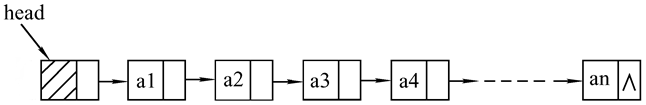
\includegraphics[width=3.36458in,height=0.55208in]{png-jpeg-pics/C20E94AE04F8208A15667A05019B1E65.png}

{b\textbf{. 双链表}\\
}

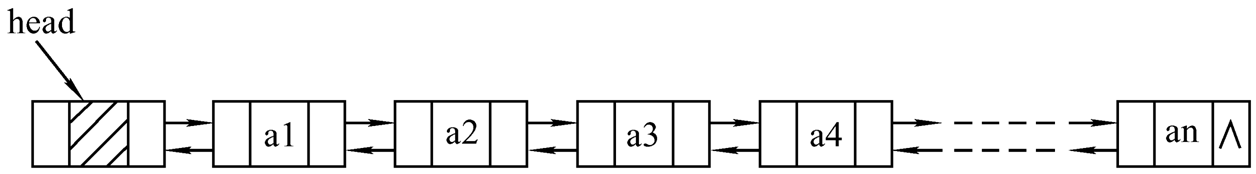
\includegraphics[width=3.33333in,height=0.45833in]{png-jpeg-pics/7D7C423781159DA1E482604156DD615A.png}

{c\textbf{. 循环单链表}\\
}

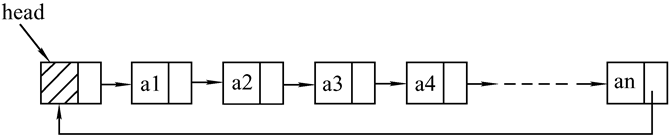
\includegraphics[width=3.48958in,height=0.71875in]{png-jpeg-pics/A73BFA643AA8FB8519FED189FD23A39C.png}

{d\textbf{. 循环双链表}\\
}

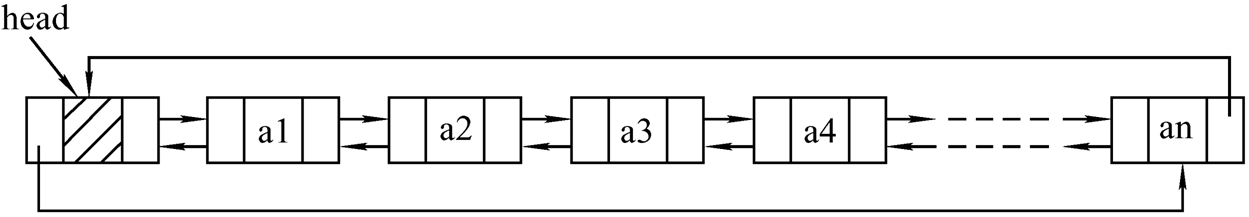
\includegraphics[width=3.33333in,height=0.58333in]{png-jpeg-pics/7E10782F7D3284B6634F5CB34D06A188.png}

{e\textbf{. 静态链表}\\
}

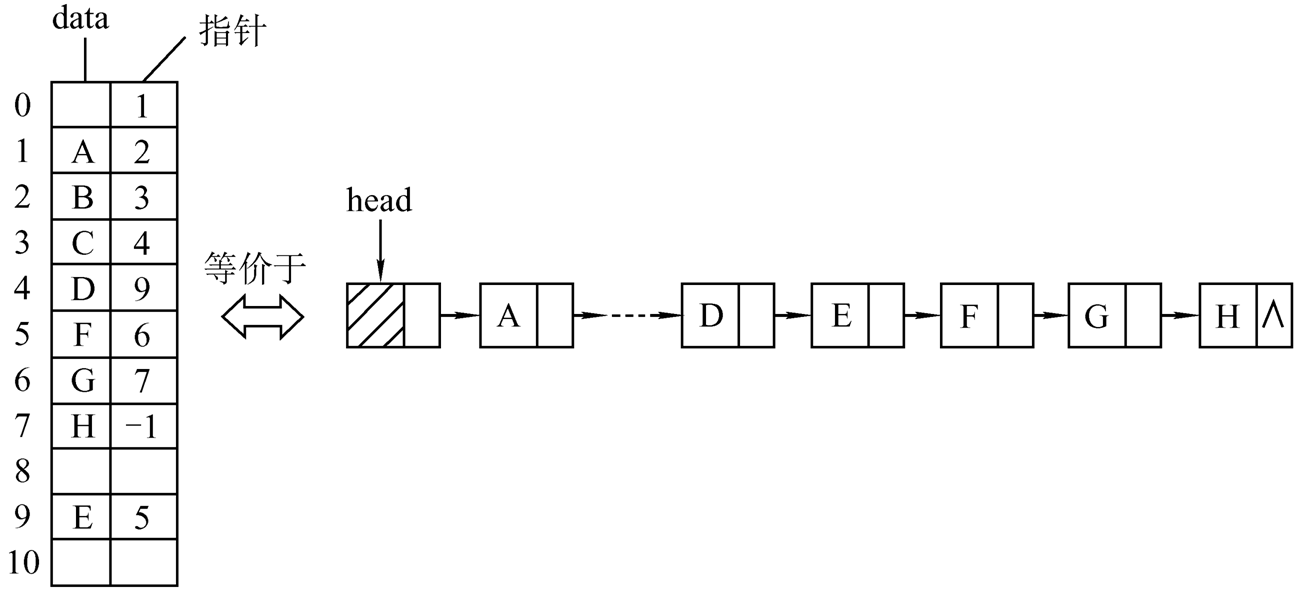
\includegraphics[width=3.33333in,height=1.51042in]{png-jpeg-pics/DBE33BB1E0A5E477AF148176D1253920.png}

\subsection{00095-线性表的定义}
线性表是具有相同特性数据元素的一个有限序列。该序列中所含元素的个数叫做线性表的长度,用n(n≥0)表示。

{\textbf{1. 顺序表的结构定义}}{}

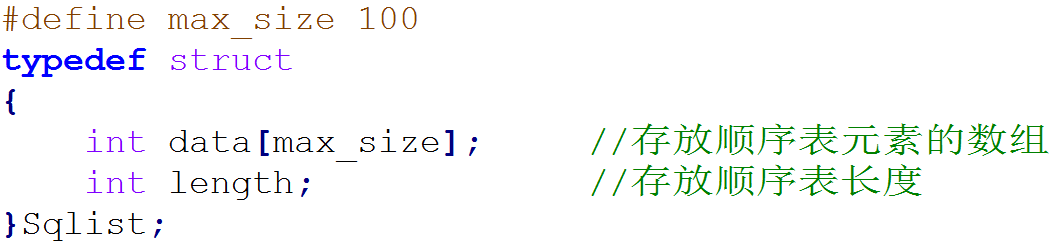
\includegraphics[width=3.33333in,height=0.77083in]{png-jpeg-pics/858F0B2FB24FD4CAC49A48E3B93C504F.png}

{上面是结构体定义,考试中直接定义数组即可。如下:\\
}

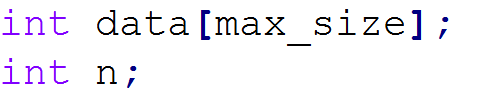
\includegraphics[width=1.25000in,height=0.22917in]{png-jpeg-pics/BB30D5618AFCED398847C5DFD44A84A8.png}

{\textbf{2. 单链表结点定义}}

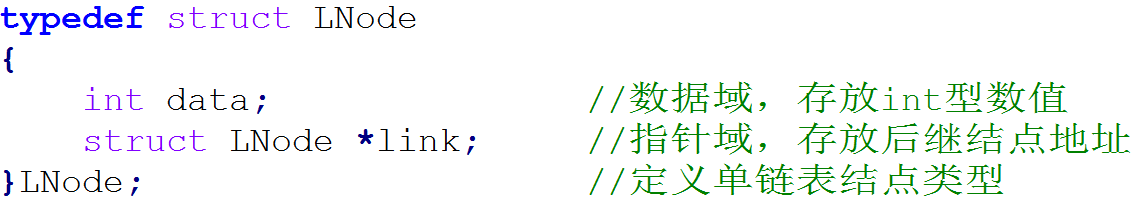
\includegraphics[width=3.33333in,height=0.58333in]{png-jpeg-pics/A6664F2AC886BAD99E87039DD7E68251.png}

{\textbf{{3. 双链表结点定义}}\\
}

{跟二叉树结点的定义很像。\\
}

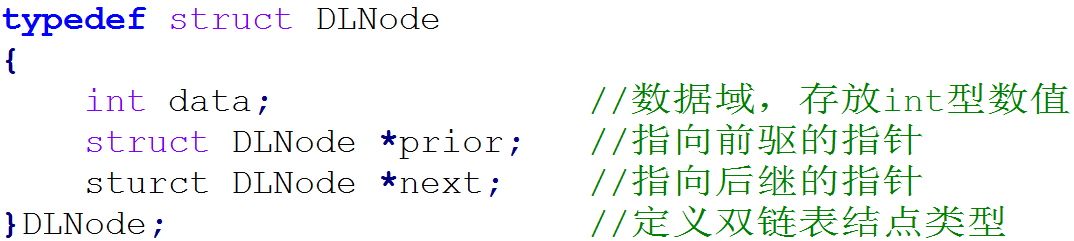
\includegraphics[width=3.33333in,height=0.75000in]{png-jpeg-pics/B2D7F23BD5AAA4BC6D2D78B5E94D4612.png}

\subsection{00096-顺序表操作}
\textbf{{1. 按下标访问顺序表元素}}

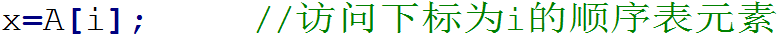
\includegraphics[width=2.18750in,height=0.10417in]{png-jpeg-pics/98374E4A1099338D04981D1ACB6B6417.png}

\textbf{{2. 按元素值的查找算法}}

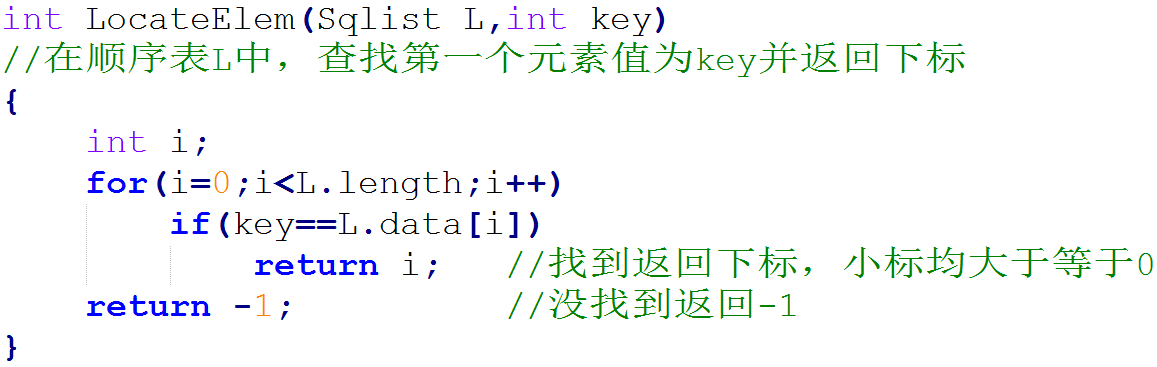
\includegraphics[width=3.33333in,height=1.06250in]{png-jpeg-pics/2F1E51D3E4237550D9FDD9DA8D0C128A.png}

\textbf{{3. 插入数据元素的算法}}

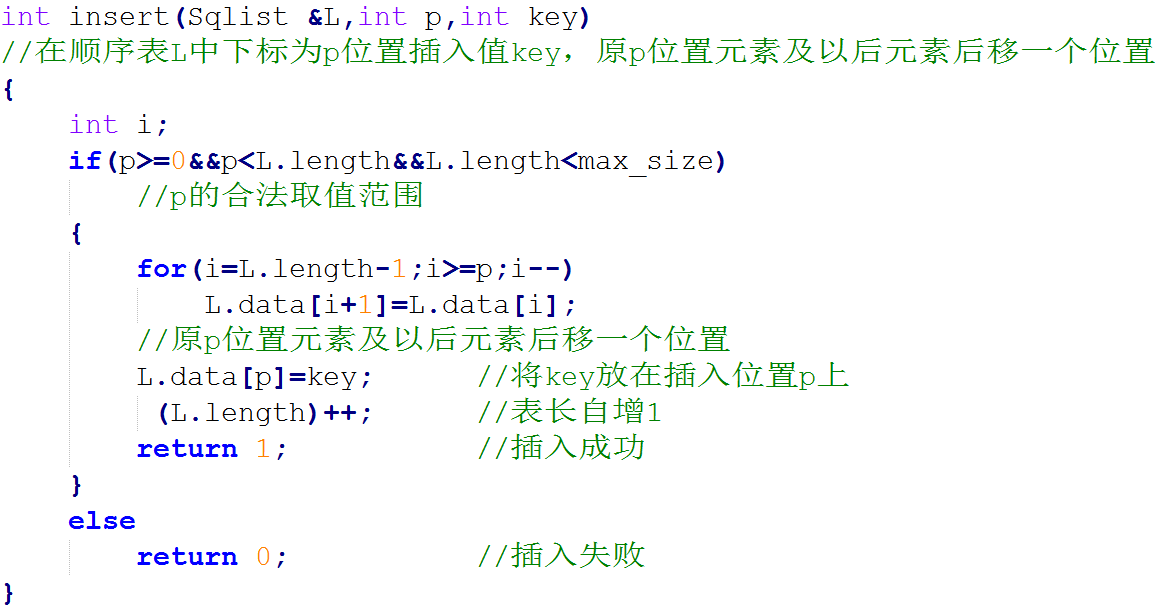
\includegraphics[width=3.33333in,height=1.75000in]{png-jpeg-pics/CD4FB43A8A96D42B741B32A293CA4082.png}

\textbf{{4. 删除数据元素的算法}}

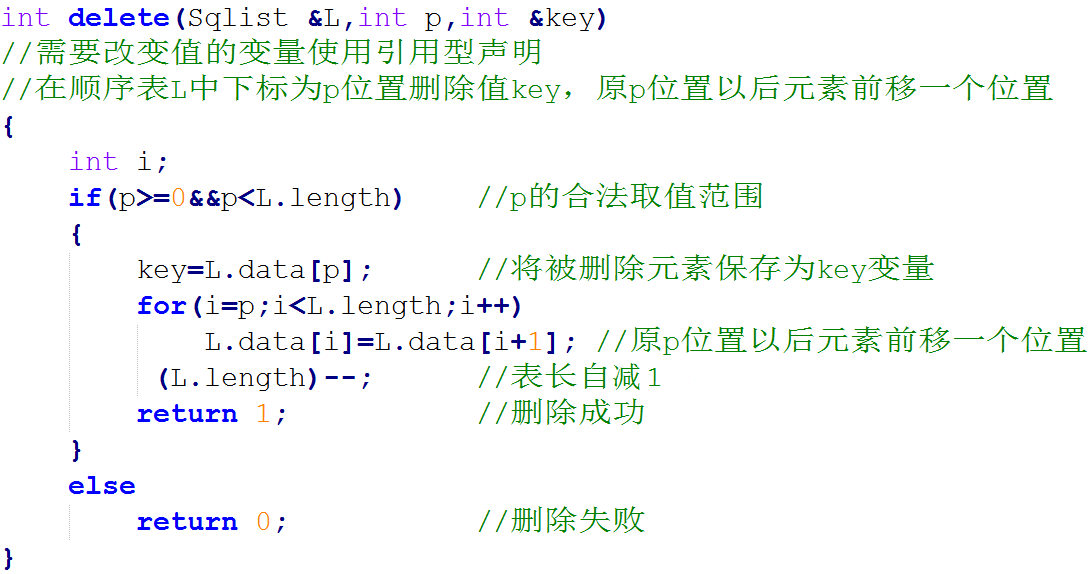
\includegraphics[width=3.12500in,height=1.64583in]{png-jpeg-pics/7633470FDBFBF6732CD62D088DFDF1A2.png}

\subsection{00097-单链表操作}
\textbf{~{1. 两个有序链表合并为一个有序链表}}

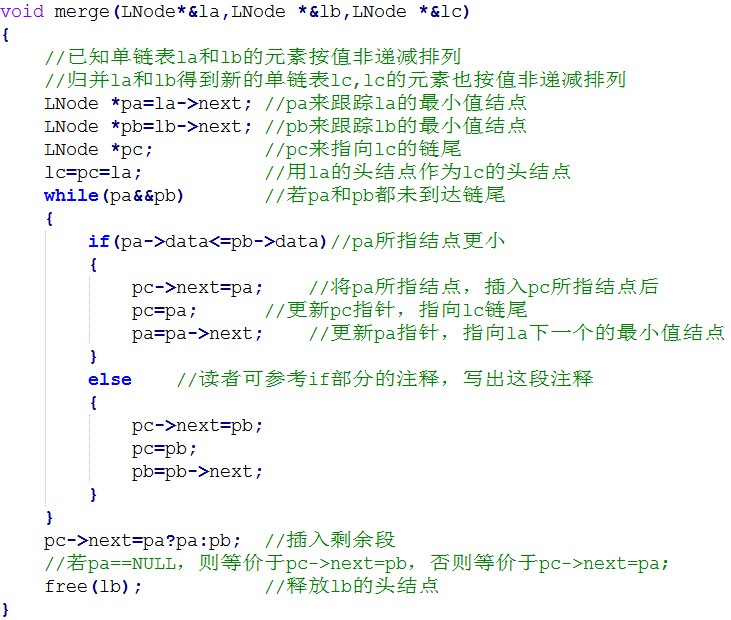
\includegraphics[width=3.12500in,height=2.64583in]{png-jpeg-pics/27B36B8E0380485A33092BEA1B313D5E.png}

\textbf{{2. 查找链表L中值为key的结点,存在就删除并返回1,否则返回0}}

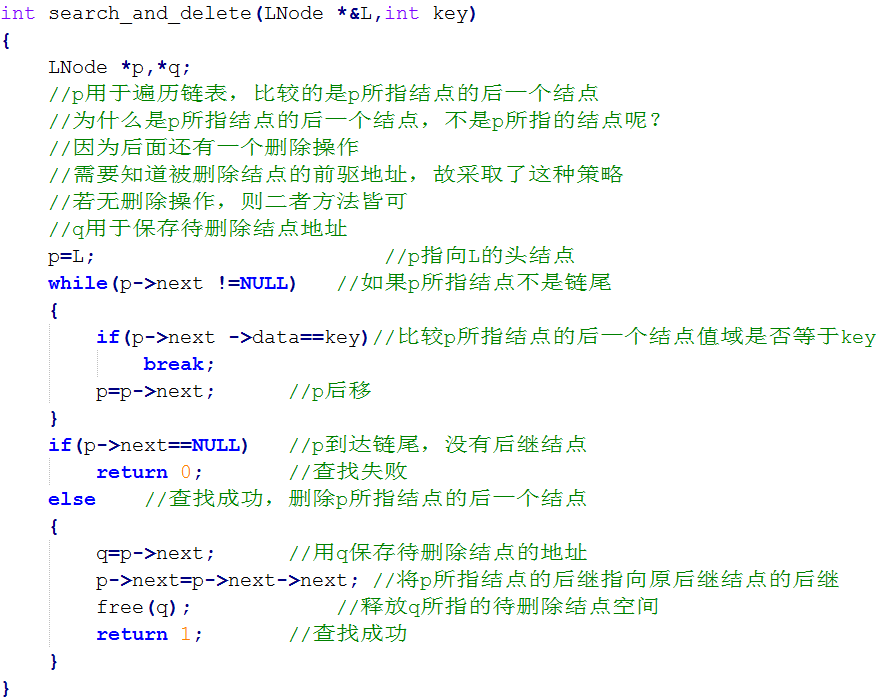
\includegraphics[width=3.22917in,height=2.56250in]{png-jpeg-pics/F334C274192073975B443739BACF94E9.png}

\subsection{00098-双链表操作}
\textbf{{1. 在双链表L尾部插入值为key的结点}}

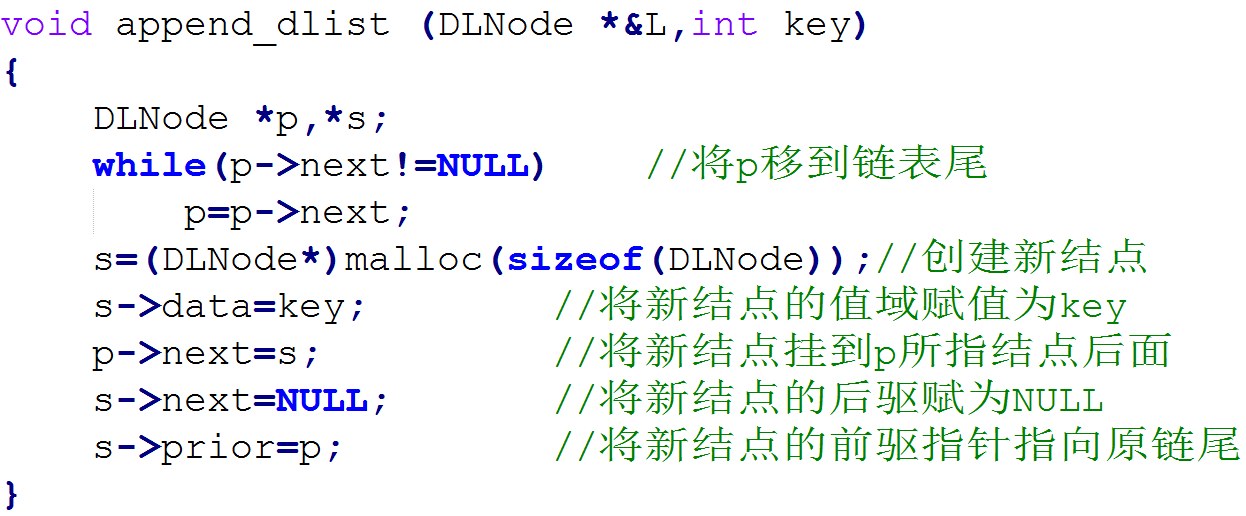
\includegraphics[width=6in]{png-jpeg-pics/03268EAA15CD33F53F293BD78E598542.png}

\textbf{{2. 查找双链表L结点值为key的结点,找到返回其地址,否则返回NULL}}

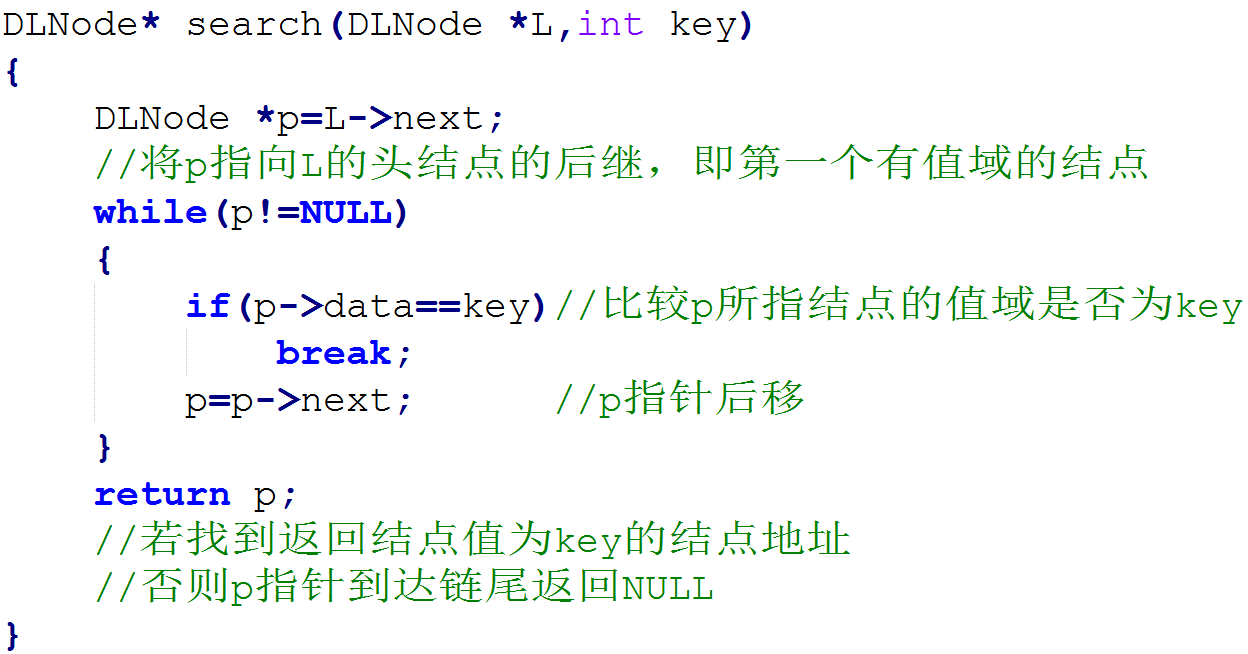
\includegraphics[width=6in]{png-jpeg-pics/01B96410D375D9482DBD49E4733D199A.png}

\textbf{{3.
在双链表中p所指结点之后插入结点s,其中p结点不是最后一个结点}}

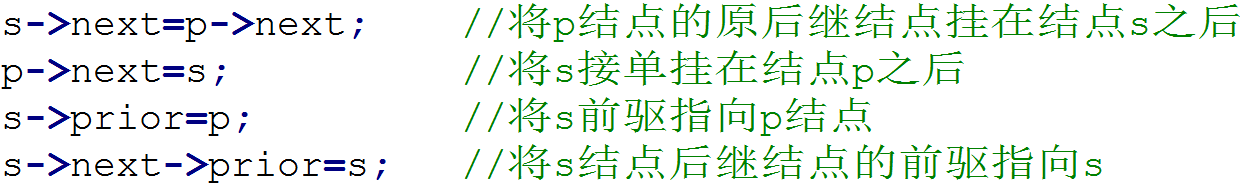
\includegraphics[width=6in]{png-jpeg-pics/1E0D67141EAF5766A73E880D92654FFF.png}

\textbf{{注意:第一行和第二行一定要记住,先写这两句,就不会错。}}

\textbf{{4. 在双链表中删除p结点的后继结点}}

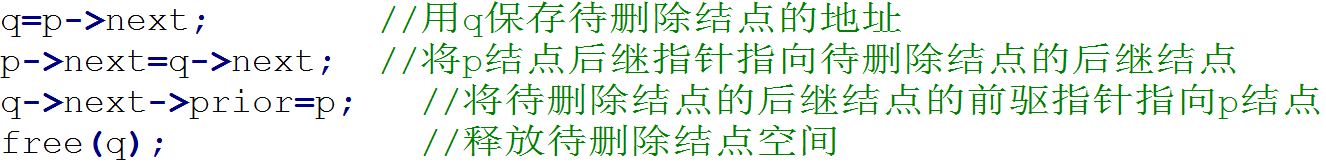
\includegraphics[width=6in]{png-jpeg-pics/5F88607817AE7DD214FE9DF244A7CE02.png}

\subsection{00099-循环链表操作}
{循环单链表和循环双链表是由对应的单链表和双链表改造而来,只需在终端结点和头结点间建立关系即可。{只需要注意一点不同,如果p指针沿着循环链表遍历,判断p遍历到表尾结点的条件变为p-\textgreater{}next==head},其余操作都与非循环链表类似。}

\subsection{00100-一元多项式的表示及相加}
{一元多项式相加的运算规则:{\textbf{对于两个一元多项式中所有指数相同的项,对应系数相加,若其和不为零,则构成``和多项式''中的一项;对于两个一元多项式中所有指数不相同的项,则分别复抄到``和多项式''中去。}}\\
用链式存储结构,实现一元多项式的相加。示意图如下:}

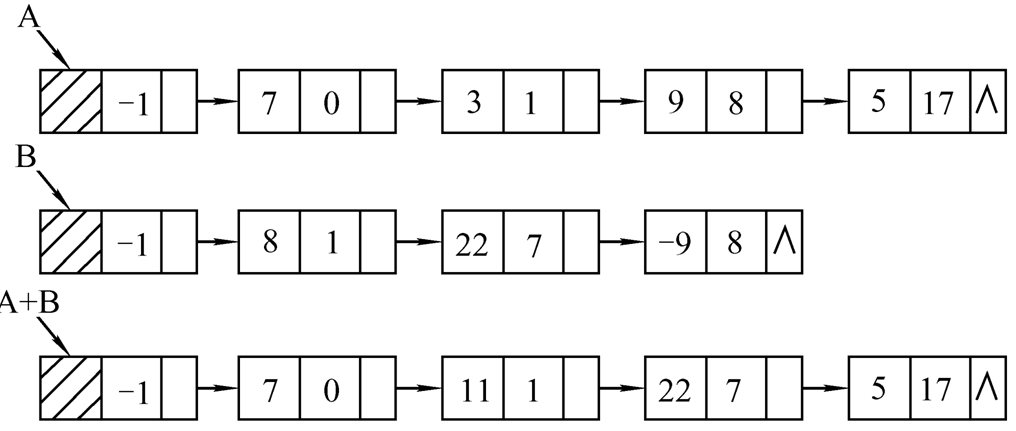
\includegraphics[width=3.22917in,height=1.37500in]{png-jpeg-pics/395B62F57E36F93B9A676676A26C7BD5.png}

{方法跟有序链表的合并有类似之处,首先对于结点的第二值域(指数),每个链表都是有序链表。如果两个一元多项式没有指数相同的项,则跟有序链表的合并是一模一样的。\\
{不同的是这里可能会有指数相同的项,多了一个相加第一值域的操作。若和不为零,则构成新的一个结点。若和为零,则两个结点``同归于尽''。}\\
考生根据这个思路和之前给的有序链表合并的代码,不难写出一元多项式的代码,由于不是重点部分,想看代码的考生请看严版教材。}

\subsection{00101-栈的定义}
栈是一种{只能在一端(栈顶)进行插入或删除操作的线性表}。插入操作称为入栈,删除操作称为出栈。

由栈的定义可得出栈的特点就是\textbf{{先进后出}}(First In Last
Out,FILO)或\textbf{{后进先出}}。

\subsection{00102-队列的定义}
{队列是一种操作受限的线性表,其限制为{允许在表的一端(队尾)进行插入(进队),而在表的另一端(队头)进行删除(出队)。}}

{由队列的定义可得出队列的特点就是\textbf{{先进先出}}(First In First
Out,FILO)或{\textbf{后进后出}}。不同的是这里可能会有指数相同的项。}

\subsection{00103-顺序栈的定义}
\textbf{1. 顺序栈的定义}

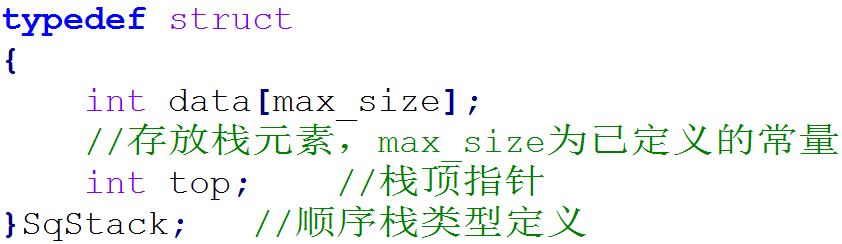
\includegraphics[width=2.81250in,height=0.81250in]{png-jpeg-pics/2808EF0D96046F76E3FF790F53B095F9.png}

考试中要用到栈的情况下,栈的声明以及操作可以写得很简单,下面给出实用的顺序栈的操作的写法:

{第一步:声明一个栈并初始化}

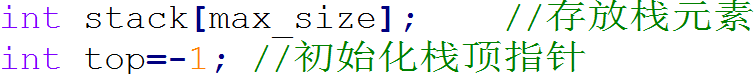
\includegraphics[width=2.39583in,height=0.23958in]{png-jpeg-pics/22CC74812EFCAA95829A01124BAA5E26.png}

{第二步:元素key入栈}

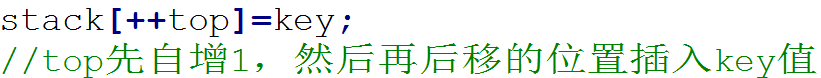
\includegraphics[width=2.62500in,height=0.25000in]{png-jpeg-pics/C052107CCE72649B9D5CC0ADBFEA8C17.png}

{第三步:出栈,值保存于变量key中}

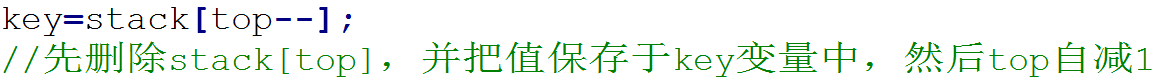
\includegraphics[width=3.33333in,height=0.23958in]{png-jpeg-pics/0800C6447573DC9A35298FF4895F511C.png}

\subsection{00104-顺序队的定义}
{\textbf{1. ~顺序队的定义}}

{\textbf{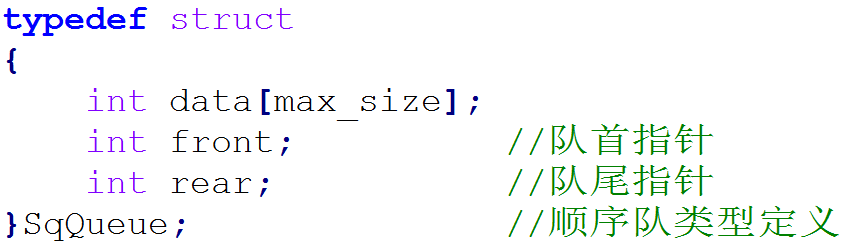
\includegraphics[width=3.12500in,height=0.90625in]{png-jpeg-pics/1D74C5110FF61D46264C806E224DEA1C.png}\\
}}

\subsection{00105-循环队列}
在顺序队列中,{通常让队尾指针rear指向队尾元素,让队首front指针指向队头元素的前一个位置。}(但这不是一定的,如2011年真题的第3道选择,就让front指向了队头元素)

为了预防rear和front都到达数组末端,造成无法让元素进队的情况,就需要把顺序队列改进为循环队列。如何实现指针的循环是一个问题,下面的语句解决了这个问题。

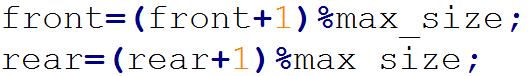
\includegraphics[width=2.39583in,height=0.34375in]{png-jpeg-pics/E027815619E166F3A6DF9E1573525F07.png}

对于循环队列两个特殊的状态,表示如下:

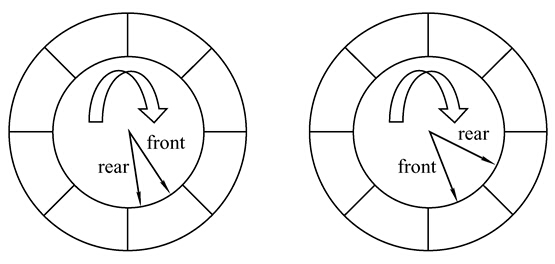
\includegraphics[width=2.08333in,height=2.08333in]{png-jpeg-pics/8616513dd4ea9ae6d81e012612d36a82?}

考生可以自己先猜一下,哪个表示队空,哪个表示队满。

由定义可知,非空位置范围其实是front指针沿顺时针方向到达rear位置,扫过的空间为队列部分。但若front和rear都指向同一位置,就不知道其为空队,还是满队了。{为了区分,循环队列必须损失一个存储空间},如右图的情况,除了front位置,其余都为非空,定为队满的情况。就不能让rear超过front一圈(就好像两个同学在400m跑道上进行长跑一样,考虑到跑慢同学的自尊心,要求跑快的同学rear不可以超过跑慢同学front一圈,即最多超过他399m,就不能再超了)。

综上,左图为队空(rear==front),右图为队满(rear+1)\%max\_size==front。

\subsection{00106-链栈的定义}
\textbf{{1. 链栈的定义}}

\textbf{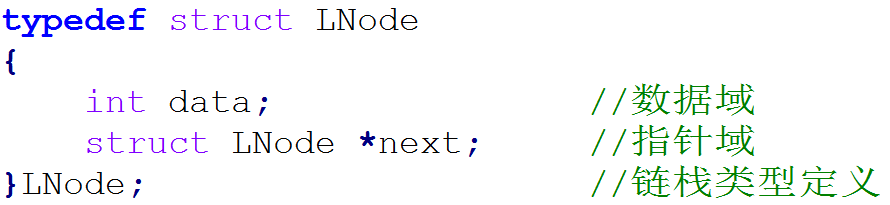
\includegraphics[width=2.81250in,height=0.64583in]{png-jpeg-pics/E67CB7E9F1DDEE7B7F76081BFC0A855F.png}\\
}

\textbf{{2. 链栈的基本操作}}

(1)入栈

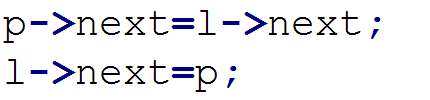
\includegraphics[width=1.35417in,height=0.31250in]{png-jpeg-pics/B40903111C8985FC06233A7AEA099426.png}

(2)出栈

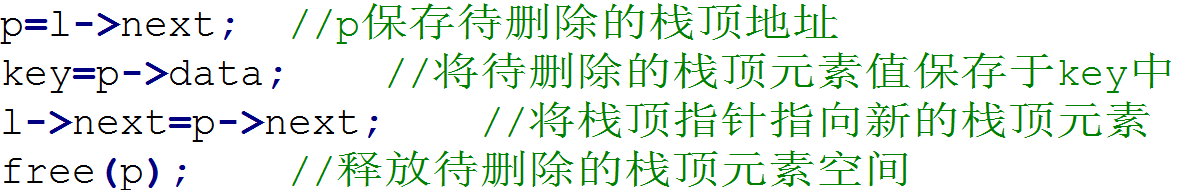
\includegraphics[width=3.43750in,height=0.55208in]{png-jpeg-pics/7FDDA5961F623A82F98AD8A1A54D51D5.png}

\subsection{00107-链队的定义}
\textbf{{1. 队结点类型定义}}

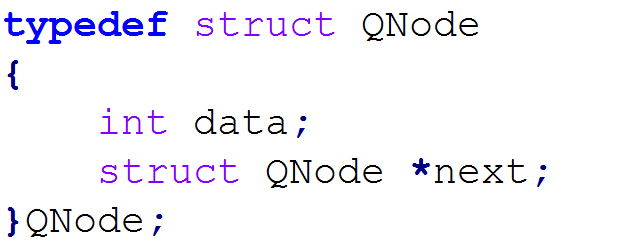
\includegraphics[width=2.08333in,height=0.79167in]{png-jpeg-pics/3B363F7937B1F95EB70FC8F952115276.png}

\textbf{2. 链队类型定义}

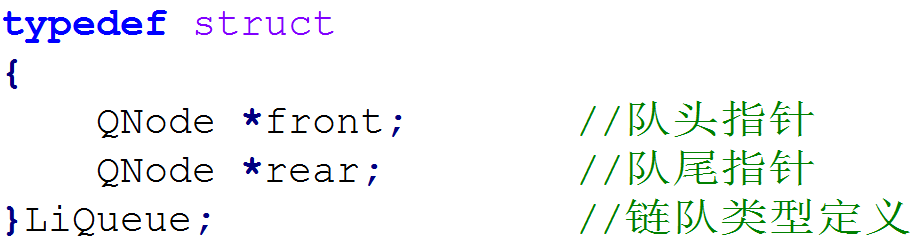
\includegraphics[width=2.81250in,height=0.73958in]{png-jpeg-pics/D2F3463CE7D9AFA2634EFAD952154C9F.png}\\

\subsection{00108-链队的队空情况}
链队有队空的情况:L-\textgreater{}rear==NULL或者L-\textgreater{}front==
NULL。

可以这样记住,因为只要链队为非空,二者值都不应该为NULL,反之为空。

链队在内存无限制的情况下,无队满的情况。

\textbf{1. 进队(类似在链表尾进行插入操作)}

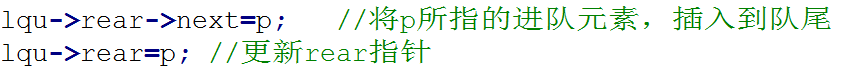
\includegraphics[width=3.59375in,height=0.29167in]{png-jpeg-pics/3206F0D598775FA50B01A619C98149DD.png}

\textbf{2. 出队(类似在链表头进行删除操作)}

\textbf{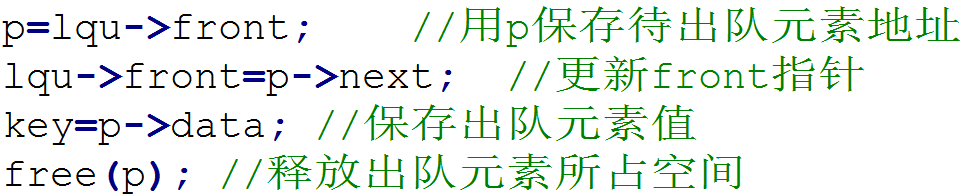
\includegraphics[width=2.91667in,height=0.59375in]{png-jpeg-pics/09CCBBEDE3B087877C02A1E27C117DF0.png}\\
}

\subsection{00109-栈的应用}
以下部分只是让考生明白,什么问题可以用栈来解决。

\textbf{{1. 数制转换}}

如十进制转换为八进制的程序,计算过程是从低位到高位顺序产生八进制的各个位数。\textbf{{而打印过程是从高位到低位进行,恰好和计算过程相反}}。因此,若将计算过程中得到的八进制数的各位依次入栈,最后按出栈序列打印输出即为与输入对应的八进制数。

\textbf{{2. 括号匹配的检验}}

考虑下列括号序列:\\
\hspace*{0.333em} ~ ~~{[} ( {[} {]} {[} {]} ) {]}

计算机接收了第一个左中括号后,期待右中括号的出现。等来的确是左小括号,此时第一个中括号必须等待,左小括号被消掉之后,才有可能被消掉,即这里\textbf{{满足了栈的``先进后出''的特点}}。用栈的处理括号的匹配时,遇左括号就进栈,遇右括号就出栈。

\textbf{{3. 行编辑程序}}

在编辑程序中,设立了一个缓冲区用于接收用户输入的一行字符,然后逐行存入用户数据区。允许用户输入出差错,并在发现有误时可以及时更正。例如用``\#''表示退格符,用``@''表示退行符。其中退格符,删除的是最后输入的字符,\textbf{{符合栈后入先出的特点}}。退行符,删除的是缓冲区全部元素。这里用栈实现很方便。{遇到普通字符,入栈。遇到退格符,栈顶元素出栈。遇到退行符,清空栈。}

\textbf{{4. 迷宫求解}}

在``穷举求解''迷宫时,为了保证在任何位置上都能沿着原路退回,显然需要用一个后进先出的结构来保存从入口到当前位置的路径。因此,在求解迷宫通路的算法中应用``栈''也就是很自然的事情。

\textbf{{5. 表达式求值}}

算法基本思想如下:

(1)首先置操作数栈为空栈,表达式起始符``\#''为运算符栈的栈底元素(为了和表达式的结束符,构成整个表达式的一对括号)。

(2)依次读入表达式每个字符,若是操作数则进OPND栈,若是运算符则和OPTR栈栈顶运算符比较优先权后作相应操作,直至整个表达式求解完毕(即OPTR栈的栈顶元素和当前读入的字符均为``\#'')。

\textbf{{6. 递归的实现(知道就行)}}

\subsection{00110-队列的应用}
队列应用的例子,其实就是需要``排队''的情形,{举例如下。}

\textbf{{1. CPU资源的竞争问题}}

{在具有多个终端的计算机系统中,有多个用户需要使用CPU各自运行自己的程}{序,它们分别通过各自终端向操作系统提出使用CPU的请求,操作系统按照每个}{请求在时间上的先后顺序,将其排成一个队列,\textbf{{每次把CPU分配给队头用户使}}}{\textbf{用,当相应的程序运行结束,则令其出队,再把CPU分配给新的队头用户,直到}}{\textbf{{所有用户任务处理完毕}}{。}}

\textbf{{2. 主机与外部设备之间速度不匹配的问题}}

以主机和打印机为例来说明(\textbf{{09年真题已经考查}}),主机输出数据给打印机打{印,主机输出数据的速度}{比打印机打印的速度要快得多,若直接把输出的数据送}{给打印机打印,由于速度}{不匹配,显然是不行的。所以解决的方法是设置一个打}{印数据缓冲区,主机把要}{打印输出的数据依次写入到这个缓冲区中,写满后就暂}{停输出,继而去做其他的}{事情,打印机就从缓冲区中按照先进先出的原则依次取}{出数据并打印,打印完后}{再向主机发出请求,主机接到请求后再向缓冲区写入打}{印数据,这样利用队列既}{保证了打印数据的正确,又使主机提高了效率。}

\subsection{00111-顺序存储}
{\textbf{1. 顺序存储}}

举2维数组的例子,同样是存储A{[}4{]}{[}5{]}中的9个元素:

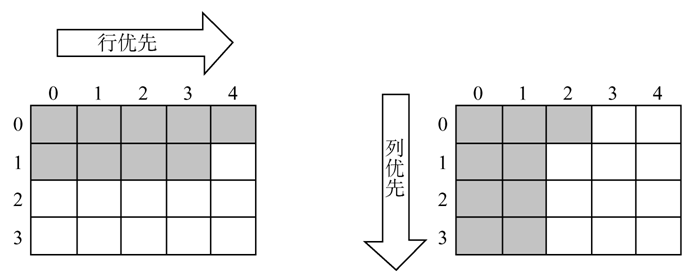
\includegraphics[width=3.12500in,height=1.22917in]{png-jpeg-pics/8C488ABCE9077951EA00275DDE50F718.png}

{a.
行优先连续存储的是A{[}0{]}{[}0~4{]}和A{[}1{]}{[}0~3{]}。}{列优先连续存储的是A{[}0~3{]}{[}0{]}、A{[}0~3{]}{[}1{]}和A{[}0{]}{[}2{]}。}

{b.
这里主要是涉及元素实际地址的计算。如给出A{[}0{]}{[}0{]}的地址求A{[}2{]}{[}3{]}的地址,在行优先和列优先就不同。}

{c.
在行优先的情况下,A{[}2{]}{[}3{]}为第14个元素,地址为A{[}0{]}{[}0{]}的地址加上13个元素空间的位移。}{在列优先的情况下,A{[}2{]}{[}3{]}为第15个元素,地址为A{[}0{]}{[}0{]}的地址加上14个元素空间的位移。}

\subsection{00112-特殊矩阵的压缩存储}
{\textbf{1. 对称矩阵}}

{将对称矩阵A压缩存储到SA{[}n(n+1)/2{]}中,aij的下标i、j与在SA中的对应元素的下标k的关系如下:}

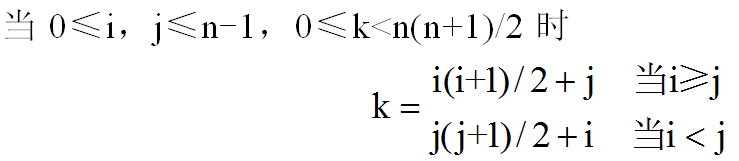
\includegraphics[width=2.50000in,height=0.54167in]{png-jpeg-pics/923EFD19FF65BD5EDFECF4ADEC3A717D.png}

{\textbf{2. 三角矩阵}}

{将上三角矩阵A压缩存储到SA{[}n(n+1)/2{]}中,aij的下标i、j与在SA中的对应元素的下标k的关系如下:}

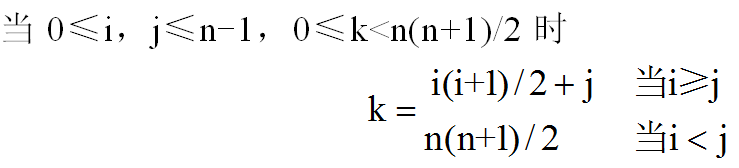
\includegraphics[width=2.39583in,height=0.54167in]{png-jpeg-pics/E7283989C6C7D818334F39947B9EEB2A.png}

{下三角{矩阵A压缩存储到SA{[}n(n+1)/2{]}中},读者可自行给出。}

{\textbf{3. 对角矩阵}}

{{所有的非零元素集中在以主对角线为中心的带状区域中},即\textbf{除了主对角线和主对角线相邻两侧的若干条对角线上的元素之外,其余元素皆为零的矩阵称为对角矩阵}。}

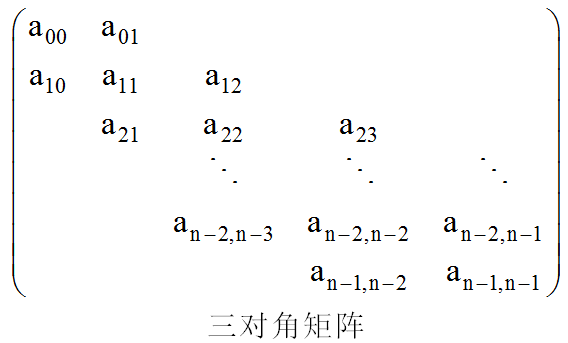
\includegraphics[width=2.29167in,height=1.38542in]{png-jpeg-pics/484F3A07CB60CCCB7EB5FBD84C919F57.png}

\subsection{00113-树相关的基本概念}
{\textbf{1. 树的基本概念}}

树是n(n≥0)个结点的有限集合T。当n=0时,称为空树;当n\textgreater{}0时,该集合满足如下条件:

{1.
其中{必有一个称为根的特定结点},它没有直接前驱,但有零个或多个直接后继(如结点a)。}

{2. 其余n-1个结点可以划分为m(m≥0)个互不相交的有限集合T1,T2,
,Tm,其中Ti又是一棵树,称为根root的子树。每棵子树的根结点有且仅有一个直接前驱,但有零个或多个直接后继。}

{\textbf{2. 树相关术语}}

{\textbf{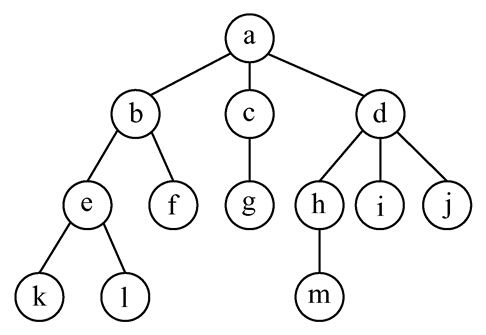
\includegraphics[width=2.08333in,height=2.08333in]{png-jpeg-pics/a16db4da9e6fde364685db7c67e3b509?}\\
}}

{1. 结点:a、b、
m都是结点,结点不仅包含数值元素,而且包含指向子树的分支。如结点a包含指向b、c、d这3个子树的指针。}

{2. 结点的度:结点拥有的子树个数(即分支个数)。如结点A的度为3。}

{3. 叶子结点(终端结点):指度为0的结点,如f、g、i、j、k、l、m。}

{4. 非终端结点:指度不为0的结点,如a、b、c、d、e、h。}

{5. 孩子:结点的子树的根,如a结点的孩子包括b、c、d这3个结点。}

{6. 双亲(父结点):如b、c、d的双亲都是a。}

{7. 兄弟:如b、c、d互为兄弟。}

{8.
祖先:从根到某结点的路径上的所有结点,都是这个结点的祖先。如k的祖先是a、b、e。}

{9.
子孙(子树结点):从某结点为根的子树中的所有结点,都是该结点的子孙。如d的子孙为h、i、j、m。}

{10. 层次:从根开始,根为第一层,根的孩子们为第二层,以此类推。}

{11.
树的高度(或深度):树中结点的最大层次。如例子中高度(或深度)为4。}

{12.
结点的深度和高度:结点深度是从根结点算起的,而结点高度是从最底层的}{叶子结点算其的。如结点g的高度为2,深度为3。}

{13.
堂兄弟:双亲在同一层(但不是同一个)的结点互为堂兄弟。如f、g、h都互为堂兄弟。}

{14.
有序树:树中结点的子树从左到右是有次序的,不能交换的,这样的树称为有序树。}

{15. 无序树:就是子树无次序,可任意交换的树称为无序树。}

{16.
森林:若干棵互不相交的树的集合。如把根A去掉,剩下的b、c、d树就组成一个森林。}

\subsection{00114-二叉树的定义}
{\textbf{1. 二叉树的定义}}

{二叉树首先是一棵树。再附加两个限制条件:}

{{条件一:} 每个结点最多只有两个子树,即二叉树中结点的度只能为0、1、2。}

{{条件二:}子树有左右之分。}{}

{\textbf{2. 满二叉树}}

{在一棵二叉树中,{如果所有的分支结点都有左孩子和右孩子结点,并且叶子结点都集中在二叉树的最后一层},这样的二叉树称为满二叉树,见下图。}

{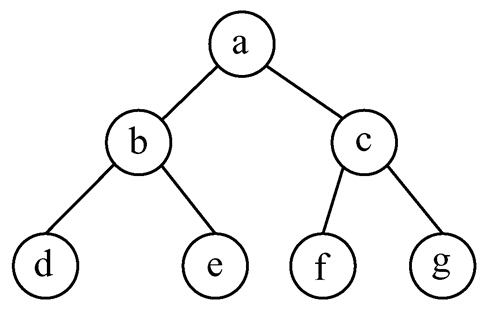
\includegraphics[width=2.08333in,height=2.08333in]{png-jpeg-pics/2168d1522cee5397fd408c62e74e19f7?}\\
\hspace*{0.333em}}

{\textbf{3. 完全二叉树}}

{若设二叉树的深度为h,除第h层外,其他各层(1~h-1)的结点数都达到最大个数,{第h层所有的结点都连续集中在最左边},这就是完全二叉树,见下图。}

{}

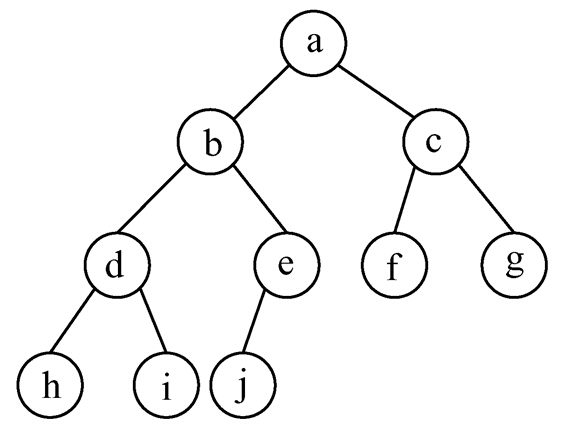
\includegraphics[width=2.08333in,height=2.08333in]{png-jpeg-pics/db52833b3034c215c5d5ec6e8ac982ed?}

\subsection{00115-二叉树的性质}
\textbf{{性质}{1}{:}}非空二叉树上叶子结点数等于双分支结点数加1。设度为i的结点个数为ni。性质1等式表示即为:n0=n2+1。

\textbf{{性质}{2}{:}}二叉树的第i层上最多有2\textsuperscript{i-1}个结点(i≥1)

\textbf{{性质}{3}{:}}高度为k的二叉树最多有2\textsuperscript{k}-1个结点(k≥1)。

\textbf{{性质}{4}{:}}有n个结点的完全二叉树,对各结点从上到下从左到有依次编号(1~n),则结点之间有如下关系:

若i为结点a的编号则:

如果i≠1,则a的双亲结点编号为
\includegraphics[width=0.33333in,height=0.17708in]{texmath/18cb1elfloori2rfloor}。

如果2×i≤n,则a有左孩子,编号为2×i,反之无左孩子。

如果2×i+1≤n,则a有右孩子,编号为2×i+1,反之无右孩子。

注:因为完全二叉树一般直接用数组存储,故通过双亲关系计算出下标的操作对完全二叉树来说是很重要的。

\textbf{{性质}{5}{:}}给定{n}个结点,能构造出
\includegraphics[width=0.88542in,height=0.18750in]{texmath/3fa64cC2nn(n+1)}{种}不同的二叉树。

\textbf{{性质}{6}{:}}具有{n}个结点的完全二叉树的深度{k}为
\textsubscript{
\includegraphics[width=0.84375in,height=0.17708in]{texmath/d2f760lfloorloglimitsrm2nrfloor+1}}或
\includegraphics[width=0.95833in,height=0.18750in]{texmath/417732lceilloglimitsrm2(n+1)rceil}。

\subsection{00116-二叉树的存储结构}
{\textbf{1. 顺序存储结构}}

{用一个数组来存储一棵二叉树,适合于完全二叉树的存储。用于存储一般二叉树则会浪费大量存储空间。将完全二叉树中的结点值按编号一次存入一个一维数组中,即完成了对一棵完全二叉树的顺序存储。}

{\textbf{2. 链式存储结构}}

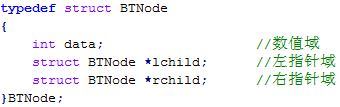
\includegraphics[width=3.54167in,height=1.11458in]{png-jpeg-pics/BEFD7EF20BBECAF465B5B19292AE6ACC.png}

\subsection{00117-二叉树的遍历算法}
{二叉树的遍历方式有{先序遍历、中序遍历、后序遍历和层次遍历}。}

{识记:这里的``先''、``中''、``后''指的都是根结点。}

{\textbf{1. 先序遍历}}

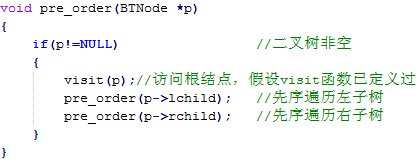
\includegraphics[width=3.70833in,height=1.42708in]{png-jpeg-pics/E4B93F3652A5B6AEA48E90F5E7B51671.png}

{\textbf{2. 中序遍历}}{}{}

\includegraphics[width=3.70833in,height=1.40625in]{png-jpeg-pics/AA7041D42D263BEB9BB27E2D52669F00.png}

{\textbf{3. 后序遍历}\\
}

\includegraphics[width=3.70833in,height=1.42708in]{png-jpeg-pics/DA6263531CC4AB6CAFCB3A75F5C3FC2A.png}

{\textbf{4. 层次遍历}}

{设二叉树的根结点所在层数为1,层序遍历就是从所在二叉树的根结点出发,首先访问第一层的树根结点,然后从左到右访问第2层上的结点,接着是第三层的结点,以此类推,{自上而下,自左至右逐层访问树的结点的过程就是层序遍历}。}

{要进行层次遍历需要建立{循环队列}。先将二叉树头结点入队列,然后出队列,访问该结点,如果它有左子树,便将左子树根结点入队,如果它有右子树,便将右子树根结点入队。然后出队列,对出队结点访问,如此反复,直到队列为空为止。}

\includegraphics[width=3.70833in,height=3.31250in]{png-jpeg-pics/324D9D425551BAABF5F198A0DB78E7A4.png}

{\textbf{扩展:}}

{\textbf{1. 求二叉树的深度,二叉树以二叉链表为存储方式}}

\includegraphics[width=3.70833in,height=1.35417in]{png-jpeg-pics/02C244175A0D32E13628EE7D835406E2.png}

{\textbf{2. 查找data域值为key的结点}\\
}

\includegraphics[width=3.70833in,height=2.13542in]{png-jpeg-pics/72561B081410F70646D1B7424340C60D.png}

\subsection{00118-二叉树的构造}
{同一棵二叉树(结点值均不相同)具有唯一的先序、中序、后序和层次序列,但不同的二叉树可能具有相同的先序、中序、后序和层次序列。{二叉树的构造就是根据提供的某些遍历序列构造二叉树的结构。}}

{关于二叉树的构造有以下几种方式,构造方法都是用递归的思想:}

{\textbf{1. 由先序序列和中序序列构造二叉树}}

{{先序:根结点(左子树的先序)(右子树的先序);中序:(左子树的中序)根结点(右子树的中序)。这样就能确定出根结点,同时又得到了左子树的先序和中序,右子树的先序和中序。继续找左右子树的根结点,直到子树的结点个数为1。构造完成。}\\
}

{\textbf{2. 由后序序列和中序序列构造二叉树}}

{{后序:(左子树的后序)(右子树的后序)根结点;中序:(左子树的中序)根结点(右子树的中序)。这样就能确定出根结点,同时又得到了左子树的后序和中序,右子树的后序和中序。继续找左右子树的根结点,直到子树的结点个数为1。构造完成。}\\
}

{\textbf{3. 由层次序列和中序序列构造二叉树}}

{这个举例会更清晰些,例如中序为DGBAECF,层次遍历为ABCDEFG。由层次遍历得知,根结点为A。再根据中序就等到DGB为左子树的中序,ECF为右子树的中序。又子树的层次遍历的结点顺序跟整棵树的层次遍历的结点顺序一致。得到左子树的层次遍历为BDG,右子树的层次遍历为CEF。这样就知道了左子树的层次和中序,右子树的层次和中序,采用同样方法即可,构造出整个二叉树。}

\subsection{00119-线索二叉树}
{n个结点的二叉链表中含有n+1个空指针域。利用二叉链表中的空指针域,存放指向结点在某种遍历次序下的前趋和后继结点的指针(这种附加的指针称为``线索'')。{这种加上了线索的二叉链表称为线索链表,相应的二叉树称为线索二叉树。}线索二叉树的结点结构定义如下:\\
}

\includegraphics[width=3.70833in,height=0.31250in]{png-jpeg-pics/2C7D92B8C8B6DFA32271B9299B2CFE31.png}

{其中:}

{~ ~ ~ ltag=0时lchild指向左子女;}

{~ ~ ~ ltag=1时lchild指向前驱;}

{~ ~ ~ rtag=0时rchild指向右子女;}

{~ ~ ~ rtag=1时rchild指向后继。}

\subsection{00120-树的存储结构}
{\textbf{1. 双亲表示法}}{}

\includegraphics[width=3.70833in,height=1.52083in]{png-jpeg-pics/4836DA8387A9B72CC5286F7A0ADCE5C4.png}

{下图为一棵树及双亲表示法的存储结构。\\
}

\includegraphics[width=3.65625in,height=1.91667in]{png-jpeg-pics/07F6C48018B2828EBF2C3AE203EC4184.png}

{\textbf{2. 孩子表示法}}

{1)假设d为树的度,采用d叉链表的存储结构,但由于很多结点的度小于d,造成很大的浪费。}

{2)把每个结点的孩子结点排列起来,看成一个线性表,且以单链表做存储结构,则n个结点有n个孩子链表。如下图所示的例子。}

\includegraphics[width=3.70833in,height=1.75000in]{png-jpeg-pics/899A3EB24E8B87B9EC2551F99D4AF3C4.png}

{\textbf{3. 孩子兄弟表示法}}

{~ ~ ~
孩子兄弟表示法又称二叉链表表示法,其实就是把树转换为二叉树,进行存储,如下图所示。}

\includegraphics[width=3.70833in,height=2.14583in]{png-jpeg-pics/5658702D90DC100F532749204A4F84F3.png}

\subsection{00121-森林与二叉树的转换}
{\textbf{1. 将树转换为二叉树}}

{{步骤1:加线。}在各兄弟结点之间用虚线相连。可理解为每个结点的兄弟指针指向它的一个兄弟。}

{{步骤2:}{删除线。}对每个结点仅保留它与其最左一个孩子的连线,删除该结点与其他孩子之间的连线。可理解为每个结点仅有一个孩子指针,让它指向自己的长子。}

{{步骤3:旋转。}把虚线改为实线从水平方向向下旋转45度,成右斜下方向。原树中实线如左斜下方向。这样就树的形状成呈现出一棵二叉树。}

{下图中a所示的树,可转换为图中d所示的二叉树。}

\includegraphics[width=3.70833in,height=1.45833in]{png-jpeg-pics/47A9E641635D85EE843D278FDFA2CB04.png}

{\textbf{2. 将一个森林转换为二叉树}}

{森林是树的有限集合,如下图a所示。由上节可知,一棵树可以转换为二叉树(没有右子树),一个森林就可以转换为二叉树(没有右子树)的森林。将森林转换为二叉树的一般步骤为:}

{{步骤1:}将森林中每棵子树转换成相应的二叉树。形成有若干二叉树的森林,如下图b所示。}

{{步骤2:}按森林图形中树的先后次序,依次将后边一棵二叉树作为前边一棵二叉树根结点的右子树,这样整个森林就生成了一棵二叉树,实际上第一棵树的根结点便是生成后的二叉树的根结点。下图是将一个森林转化为一棵二叉树的示例。图中d是转化后的一棵二叉树。下图中,图中a包含三棵树的森林可转换为图中d所示的二叉树。}

{\includegraphics[width=3.70833in,height=2.73958in]{png-jpeg-pics/8E1BB4B1D59EC35B61044A5A4531A9DF.png}\\
}

{\textbf{3. 二叉树转换为一般树}}

{此时的二叉树必须是由某一树(一般树)转换而来的没有右子树的二叉树。并非随便一棵二叉树都能还原成一般树。}

{其还原过程也分为三步:}

{{步骤1:加线。}若某结点i是双亲结点的左孩子,则将该结点i的右孩子以及当且仅当连续地沿着右孩子的右链不断搜索到所有右孩子,都分别与结点i的双亲结点用虚线连接。}

{{步骤2:删除线。}把原二叉树中所有双亲结点与其右孩子的连线删除。这里的右孩子实质上是原一般树中结点的兄弟,删除的连线是兄弟间的关系。}

{{步骤3:进行整理。}把虚线改为实线,把结点按层次排列。}

{下图是把二叉树还原为一般树。}

{\includegraphics[width=3.70833in,height=1.95833in]{png-jpeg-pics/61F1D65B8B45C7E8E61FD9B3735B636C.png}\\
}

{}

{\textbf{4. 二叉树转换为森林}}

{将一棵二叉树转化成森林,可按如下步骤进行:}

{删除线:将二叉树根结点与其右孩子之间的连线,以及沿着此右孩子的右链连续不断搜索到的右孩子间的连线删除。这样就得到了若干棵根结点没有右子树的二叉树。将得到的这些二叉树用前述方法分别转化成一般树。}

\subsection{00122-树和森林的遍历}
{\textbf{1. 树的遍历}}{}

{树的遍历有两种方式:先根遍历和后根遍历。}

{{先根遍历}是先访问根结点,再依次访问根结点的每棵子树,访问子树时仍遵循先根再子树的规则。比如下图中的树进行先根遍历为:abeklfcgdhmij。}{}

{{后根遍历}是先依次访问根结点的每棵子树,再访问根结点,访问子树时仍遵循先子树再根的规则。比如下图中的树进行后根遍历为:klefbgcmhijda。}{}

{\includegraphics[width=2.08333in,height=2.08333in]{png-jpeg-pics/37d56eb30a4029dd9d455d19b9f4b080?}}

{\textbf{2. 森林的遍历}}

{森林的遍历有两种方式:先序遍历和后序遍历。}

{先序遍历森林}

{~ ~ ~ 若森林非空,则按下述规则遍历:}

{~ ~ ~~1)访问森林中第一棵树的根结点。}

{~ ~ ~ 2)先序遍历第一棵树中根结点的子树森林。}

{~ ~ ~ 3)先序遍历除去第一棵树之后剩余的树构成的森林。}

{~ ~ ~ 比如下图中的森林,先序遍历为:ABCDEFGHIJ。}

{中序遍历森林}

{~ ~ ~~若森林非空,则按下述规则遍历:}

{~ ~ ~ 1)中序遍历森林中第一棵树的根结点的子树森林。}

{~ ~ ~ 2)访问第一棵树的根结点。}

{~ ~ ~ 3)中序遍历除去第一棵树之后剩余的树构成的森林。}

{~ ~ ~ 比如下图中的森林,中序遍历为:BCDAFEHJIG。}

{\includegraphics[width=2.08333in,height=2.08333in]{png-jpeg-pics/2a35ee42c99c72c88bb6a823cadca23d?}}

\subsection{00123-二叉排序树}
{\textbf{1. 二叉排序树定义}}

{二叉排序树或者是空树,或者是满足如下性质的二叉树:}

{~(1)若它的左子树不为空,则左子树上所有关键字的值均小于根关键字的值。}

{~(2)若它的右子树不为空,则右子树上所有关键字的值均大于根关键字的值。}

{~(3)左右子树均为一棵二叉排序树。}

{如果输出二叉排序树的中序遍历序列,则它这个序列是递增有序的。}

{\textbf{2. 查找关键字}}

\includegraphics[width=3.70833in,height=2.63542in]{png-jpeg-pics/8CE04083F835D119A23665EED821C55A.png}

{\textbf{3. 插入关键字}}

{对查找关键字的算法进行修改即能完成插入关键字的算法。}

\includegraphics[width=3.70833in,height=3.43750in]{png-jpeg-pics/EAFA52E772727C988A107FA033D79A31.png}

{\textbf{4. 删除关键字}}

{假设在二叉排序树上被删除结点为p,f为其双亲结点,则删除结点p的过程分为3种情况:}

{(1)若p结点为叶子结点,直接删除即可。}

{(2)若p结点只有右子树而无左子树,或者只有左子树而无右子树。只需把p删掉,将p的子树直接连接在原来p与其双亲结点f相连的指针上即可。}

{(3)若p结点既有左子树又有右子树。}

{沿p的左子树根结点的右指针一直往右,直到右子树的最右边的结点r。将p的关键字用r中的关键字代替。最后判断,如果r是叶子结点按1)方法删除,若r是非叶子结点,则按2)方法删除r。}

\subsection{00124-平衡二叉树}
{\textbf{1. 平衡二叉树的概念}}

{平衡二叉树(AVL树)是一种特殊的二叉排序树。{其左右子树都是平衡二叉树,且左右子树高度之差的绝对值不超过1}。也可以表述为:以树中所有结点为根的树的左右子树高度之差的绝对值(平衡因子)不超过1。}

{\textbf{2. 平衡二叉树的插入}}

{前面跟二叉排序树的插入一样,就是在插入新的关键字后要进行检查,看新关键字的插入是否会使原平衡二叉树失去平衡,若失去平衡,就要进行平衡调整。}

{当失去平衡的最小子树被调整为平衡子树的时候,原有其他所有不平衡子树无需调整,整个二叉排序树就会成为一棵平衡二叉树。}

失去平衡的最小子树就是以距离插入结点最近,且平衡因子等于2或-2的结点作为根的子树。平衡调整有4种情况,分别为LL型、RR型、LR型和RL型。举例如下,以关键字序列\{16,3,7,11,9,26,18\}构造一棵平衡二叉树,如下图所示。

\includegraphics[width=3.70833in,height=2.56250in]{png-jpeg-pics/38C3C4968C61359952421C25368E97F4.png}

{\textbf{3. 平衡二叉树的删除}}

{前面与二叉排序树的删除一样,就是在删除关键字后要进行检查,看新关键字的插入是否会使原平衡二叉树失去平衡,若失去平衡,就要进行平衡调整。}

\subsection{00125-赫夫曼树和赫夫曼编码}
{\textbf{1. 赫夫曼树}}

{{赫夫曼树又称最优二叉树,是一种带权路径长度最短的二叉树}。所谓树的带权路径长度,就是树中所有的叶结点的权值乘上其到根结点的路径长度(路径长度即路径上的分支数)。树的带权路径长度记为:}

\includegraphics[width=3.70833in,height=0.68750in]{png-jpeg-pics/55D22CD2B0D12A01E2475DA33D5F35E2.png}

{\textbf{2. 构造赫夫曼树的方法}}

{{第一步:}将给定的n个权值分别看成只有根的n棵二叉树,这些二叉树构成的集合记为F。}

{{第二步:}从F中选出两棵根结点的权值最小的树(假设a和b)作为左右子树构造一棵新的二叉树(假设为c),新的二叉树的根结点的权值为左右子树根结点权值之和。}

{{第三步:}从F中删除a和b,加入c。}

{{第四步:}重复第二步和第三步,直到F中只剩下一棵树为止,这棵树便是要遍历的赫夫曼树。}

{\textbf{3. 对赫夫曼树的性质总结}}

{{性质1:}用n个权值的赫夫曼树,需要n-1次合并。}

{{性质2:}赫夫曼树中只有度为0和2的结点。}

{{性质3:}n个权值对应的赫夫曼树不唯一。}

{{性质4:}{深度为h的赫夫曼树,最大编码长度为h-1。}}

{{性质5:}{赫夫曼编码是能使电文代码总长最短的编码方式。}}

{{{性质6:}赫夫曼是一种前缀编码(就是任一字符的编码,都不是另一个字符编码的前缀)。}}

{\textbf{4. 赫夫曼编码}}

{根据给定字符值求赫夫曼编码的过程,实质就是根据给定权值构造赫夫曼树的过程。以a、b、c、d的出现频率为0.4、0.3、0.1、0.2为例,求赫夫曼编码过程如下:}

{{第一步:}根据权值构造赫夫曼树。}

{{第二步:}对构造好的赫夫曼树,约定左分支为0,右分支为1。}

{{第三步:}从根结点到叶子结点的分支上的编码组成该叶子结点的赫夫曼编码,A为0,B为10,C为110,D为111,如下图所示。}

{\includegraphics[width=2.08333in,height=2.08333in]{png-jpeg-pics/bb7b22b1f9410526bd709b8b58bf6702?}}

\subsection{00126-图相关的基本概念}
{\textbf{(1)图:}图是有结点的有穷集合V和边的集合E组成。}

{\textbf{(2)有向图和无向图:}有向图每条边都有方向,无向图每条边都没有方向。}

{\textbf{(3)弧:}有向图中,边称为弧,记为\textless{}v\textsubscript{i},v\textsubscript{j}\textgreater{},表示一条从顶点{v}\textsubscript{i}到顶点{v}\textsubscript{j}的边。}

{\textbf{(4)顶点的度、入度和出度:}与顶点v相关的边数称为顶点v的度。入度和出度都是有向图的概念。在有向图中指向顶点v的边数称为顶点v的入度,由顶点v发出的边数称为顶点v的出度。}

{\textbf{(5)有向完全图和无向完全图:}有向图最多有n(n-1)条边,称这样具有n(n-1)条边的有向图为有向完全图。无向图最多有n(n-1)/2条边,称这样具有n(n-1)/2条边的无向图为无向完全图。}

{\textbf{(6)路径和路径长度:}路径即为相邻顶点序偶构成的序列,如\textless{}a,b\textgreater{},\textless{}b,c\textgreater{}构成一条路径。路径长度指路径上边的数目。}

{\textbf{(7)简单路径:}路径序列中顶点和边都不重复出现的路径为简单路径。}

{\textbf{(8)回路:}一条路径第一个顶点和最后一个顶点相同,称为回路。}

{\textbf{(9)无向图的连通、连通图和连通分量:}这3个概念都是针对无向图的。从顶点{v}\textsubscript{i}到顶点{v}\textsubscript{j}有路径,称{v}\textsubscript{i}和{v}\textsubscript{j}连通。任意两个顶点之间都连通,成为连通图。否则,将其中最大的极大连通子图称为连通分量。}

{\textbf{(10)有向图的连通、强连通图和强连通分量:}这3个概念都是针对有向图的。从顶点{v}\textsubscript{i}到vj有路径,称{v}\textsubscript{i}和{v}\textsubscript{j}连通。对于每一对顶点{v}\textsubscript{i}和{v}\textsubscript{j},从{v}\textsubscript{i}到{v}\textsubscript{j}和{v}\textsubscript{j}到{v}\textsubscript{i}都有路径,称该图为强连通图。否则,将其中极大强连通子图称为强连通分量。}

{\textbf{(11)权和网:}图中每条边都可以有值,用于表示从一个顶点到另一个顶点的距离(代价),该数值称为权。{边上带权的图称为带权图,也称为网。}}

\subsection{00127-图的存储结构}
{\textbf{1. 邻接矩阵}}

{邻接矩阵是图的顺序存储结构。A{[}i{]}{[}j{]}=1表示顶点i到顶点j存在边或弧。A{[}i{]}{[}j{]}=0则没有,}{如下图所示。}

{\includegraphics[width=3.71875in,height=1.60417in]{png-jpeg-pics/56BEF531A2AC657890949C5D11585A83.png}\\
}

{邻接矩阵的结构型定义如下:}{}{}{~}

\includegraphics[width=3.70833in,height=1.63542in]{png-jpeg-pics/4FD252811BCF77D0A40599876B04AFB9.png}

{\textbf{2. 邻接表}}

{邻接表是图的链式存储结构。对每个顶点建立一个单链表,每个单链表的第一个结点存放顶点信息,其余结点存放边信息。如下图所示。}

{\includegraphics[width=3.70833in,height=2.06250in]{png-jpeg-pics/9403C7B366EB7BD65BE09160658072C6.png}\\
}{邻接表存储表示的定义如下:}

\includegraphics[width=3.70833in,height=2.65625in]{png-jpeg-pics/FBBDB091E668B536041132EA0D998D47.png}

\subsection{00128-图的遍历}
{\textbf{1. 深度优先搜索遍历(DFS)}}

{从图中的某结点v开始访问,访问他的任意一个邻结点w1;再从w1出发,访问与w1邻接但是没有被访问过的结点w2;然后再从w2出发,进行类似的访问\ldots{}\ldots{},如此进行下去,当一个顶点的所有邻接结点都被访问过时,则依次退回到前一次刚访问过的结点,看是否还有其他没有被访问的邻接结点。如果有,则访问此结点,然后再从此结点出发,进行与前述类似的访问。重复上述过程,直到连通图中所以结点都被访问过为止。}

{图的深度优先搜索遍历类似于二叉树的先序遍历,唯一的区别在于:{二叉树的先序遍历对于每个结点要递归地访问两个分支,图的深度优先搜索遍历则是要递归地访问多个分支。}}

{以邻接表为存储结构的深度优先搜索遍历算法:}

\includegraphics[width=3.70833in,height=1.73958in]{png-jpeg-pics/707E925EDD4194753E9B149C6EFC6D8E.png}

{\textbf{2. 广度优先搜索遍历(BFS)}}

{从图中某个顶点v出发,并访问该顶点,然后访问v的各个未曾被访问的邻接点w1,w2,\ldots{}
,wk,然后依次从w1,w2,\ldots{}
,wk出发访问各自未被访问的邻接点。重复步骤2,直到全部顶点都被访问为止。}

{以邻接表为存储结构的广度优先搜索遍历算法:}

\includegraphics[width=3.70833in,height=2.91667in]{png-jpeg-pics/7BFE384E1625FF63709604A860D8BAAF.png}

\subsection{00129-最小(代价)生成树}
{最小生成树是{一个有n个结点的连通图的生成树是原图的极小连通子图,且包含原图中的所有n个结点,并且有保持图连通的最少的边。}}

{最小生成树的总结:}

{性质1:使用不同的遍历图的方法,可以得到不同的生成树;从不同的顶点出发,也可能得到不同的生成树。}

{性质2:按照生成树的定义,n个顶点的连通网络的生成树有n个顶点、n-1条边。}

{性质3:构造最小生成树的准则:}

{①必须使用且仅使用该网络中的n-1条边来连接网络中的n个顶点;}

{②不能使用产生回路的边;}

{③各边上的权值的总和达到最小。}

{\textbf{2. 普里姆算法}}

{从连通网络N=\{V,E\}中的某一顶点u出发,选择与它关联的具有最小权值的边(u,v),将其顶点加入到生成树顶点集合U中。以后每一步从一个顶点在U中,而另一个顶点不在U中的各条边中选择权值最小的边(u,v),把它的顶点加入到集合U中。如此继续下去,直到网络中的所有顶点都加入到生成树顶点集合U中为止(读者可以用下图所示的例子实践一下,明白过程即可,一般考研试卷不直接考查代码实现)。}

\includegraphics[width=3.70833in,height=2.32292in]{png-jpeg-pics/D43193B0360B43E38FBD1456AE03CDF3.png}

{总结:}

{(1)普里姆算法的复杂度为O(n\textsuperscript{2})。}

{(2){普里姆算法适用于稠密图}。}

% {\\
% }

{\textbf{2. 克鲁斯卡尔算法}}

{将下图中边按权值从小到大排序,然后从最小边开始扫描,并检测当前边是否为候选边(即是否该边的并入会构成回路),如不构成回路,则将该边并入当前生成树中,直到所有边都被检测完为止。(读者可以用如下图所示的例子实践一下,明白过程即可,一般考研试卷不直接考查代码实现)}

{\includegraphics[width=3.70833in,height=2.59375in]{png-jpeg-pics/07BF7741A39C5FE66EBE18C782A6EC16.png}\\
\hspace*{0.333em}}

{总结:}

{(1)复杂度取决于排序算法。}

{(2)克鲁斯卡尔算法适用于稀疏图。}

\subsection{00130-最短路径}
{最短路径问题是图论研究中的一个经典算法问题,{旨在寻找图(由结点和路径组成的)中两结点之间的最短路径}。算法具体的形式包括:}

{{第一种:}{迪杰斯特拉算法}{,}此算法是一种}{确定起点求最短路径的问题。}

{{{第二种:}{弗洛伊德算法}{,}此算法是求图中任意一对顶点间的最短路径。}}

{\textbf{1. 迪杰斯特拉算法}}

\includegraphics[width=3.70833in,height=1.02083in]{png-jpeg-pics/F5BB29135CB5BF3A38D4436EC07F7F87.png}

{}

{\includegraphics[width=3.70833in,height=3.14583in]{png-jpeg-pics/5A3D0661340FA3AE873B2E5D0908E9F7.png}\\
}

{\textbf{2. 弗洛伊德算法(可选看,掌握\textbf{迪杰斯特拉算法}即可)}}

{\textbf{\includegraphics[width=3.70833in,height=1.51042in]{png-jpeg-pics/100728F2DD647E5541BAE5A9650BCE86.png}\\
}}

{\textbf{\includegraphics[width=3.70833in,height=5.61458in]{png-jpeg-pics/FCB984767E7C573FB82B60E31CC8018E.png}\\
}}

{\textbf{\includegraphics[width=3.70833in,height=0.54167in]{png-jpeg-pics/7B265A48E834B4FFEE752E6EDF63F26C.png}\\
}}

{\textbf{\includegraphics[width=3.70833in,height=2.94792in]{png-jpeg-pics/E05C0079C0652F8DAB296970044FA836.png}\\
}}

\subsection{00131-拓扑排序}
{AOV(Activity On Vertex
network)网{是一种顶点表示活动,边表示活动的先后次序,没有回路的有向图。}}

{对一个有向无环图G进行拓扑排序,是将G中所有顶点排成一个线性序列,使得图中任意一对顶点u和v,若存在从u到v的路径,则u在线性序列中出现在v之前。}

{拓扑排序的步骤为:}

{1. 在有向图中选一个没有前驱的顶点并且输出之。}

{2. 从图中删除该顶点和所有以它为尾的弧。}

{3.
重复上述两步,直至全部顶点均已输出或图中剩余的顶点中都有前驱。后者说明有向图中有环。}

{{\textbf{由于没有前驱的顶点可能不唯一,所以拓扑排序的结果也不唯一,}}如下图所示。}

{\includegraphics[width=3.70833in,height=4.72917in]{png-jpeg-pics/1BE46EE02D14AF09C8488846718668CB.png}\\
\hspace*{0.333em}}

{故本例有3个不同的拓扑排序序列,分别为:abced、abecd、aebcd。}

\subsection{00132-关键路径}
{AOE(Activity On Edge
network)网的{边表示活动,边有权值代表活动持续时间,顶点表示事件,事件是图中新活动开始或者旧活动结束的标志。}}

{在AOE网络中,{\textbf{从源点到汇点的所有路径中,具有最大路径长度的路径称为关键路径}}。关键路径代表了整个工程所完成的\textbf{{最短时间}}。这么理解吧,工程的各个段是可以并行进行的,即使这个工程并行程度足够高,最长路径代表了工程至少需要的完成时间。}

{求关键路径的一般方法:}

\includegraphics[width=3.70833in,height=2.15625in]{png-jpeg-pics/E7061CD56D902F653AFC2CAED02064D4.png}

\subsection{00134-顺序查找法}
{{算法要求:}必须采用顺序存储结构。}

{{基本思路:}从表的一端开始,顺序扫描线性表,依次将扫描到的关键字和给定值k比较,若当前扫描的关键字与k相等,则查找成功;若扫描结束后,仍未有关键字与k相等,则查找失败。代码实现非常简单,如下:}{}

\includegraphics[width=3.70833in,height=1.69792in]{png-jpeg-pics/A6443AB171562CF2863483C88E45019D.png}

\subsection{00135-分块查找}
{\textbf{1. 概念描述}}

{{分块查找又称为索引顺序查找},其数据结构可以简单描述为:分块查找把线性表分成若干块,{每一块中元素的存储顺序是任意的,但是块与块之间必须按照关键字大小有序排列},即前一块中的最大关键字要小于后一块中的最小关键字。对顺序表进行分块查找需要额外建立一个索引表,表中的每一项对应线性表中的一块。}{索引表的定义如下:}

\includegraphics[width=3.70833in,height=0.80208in]{png-jpeg-pics/7B6353AA0580E0C833864C13ECA0965F.png}

{\textbf{~2. 算法描述}}

{分块查找算法非常简单,可以分为两步进行,{首先确定待查找的元素属于哪一块,然后在块内精确查找该元素}。由于索引表是递增有序的,因此第一步采用二分查找。块内元素一般个数较少,因此第二步采用顺序查找即可。}

分块查找实际上进行{\textbf{两次查找}},{整个算法的平均查找长度是两次查找的平均查找的平均查找长度之和},即二分查找平均查找长度+顺序查找平均查找长度。

~ ~ ~ ~

\subsection{00136-折半查找法}
{{算法要求:}}

{① 必须采用顺序存储结构;}

{② 必须按关键字大小有序排列。}

{{基本思路:}首先,假设表中元素是按升序排列,将表中间位置记录的关键字与查找关键字比较,如果两者相等,则查找成功;否则利用中间位置记录将表分成前、后两个子表,如果中间位置记录的关键字大于查找关键字,则进一步查找前一子表,否则进一步查找后一子表。重复以上过程,直到找到满足条件的记录,使查找成功,或直到子表不存在为止,此时查找不成功。对应代码也并不难,如下:}

\includegraphics[width=3.70833in,height=1.72917in]{png-jpeg-pics/528BA045C8243E9DF3749442524992A9.png}

\subsection{00137-B-树}
\input{studypoints-chapters/00137-B-树}
\subsection{00138-B+树}
\input{studypoints-chapters/00138-B+树}
\subsection{00139-散列表}
{\textbf{1. 概念}}

{散列表就是根据给定的关键字来计算出关键字在表中的地址。}

{\textbf{2. 构造}}

{常用的Hash函数的构造方法}

{(1)直接定址法}

{~即H(key)=key或H(key)=a*key+b}

{(2)数字分析法}

{假设关键字是r进制,并且Hash表中可能出现的关键字都事先知道,则去关键字的若干位数组成散列地址。}

{(3)平方取中法}

{取关键字平方后的中间几位为散列地址。}

{(4)除留余数法}

{即H(key)=key mod
p,{一般p选择小于或者等于表长的最大素数},这样可以减少冲突。}

{\textbf{3. 冲突处理}}

{冲突:因为Hash函数的关系,常常会发生多个关键字共用一个地址的情况,这种情况就称为冲突。冲突处理就是为共用一个地址的关键字找到另一个``空''的散列地址。}

\includegraphics[width=3.70833in,height=1.81250in]{png-jpeg-pics/AB38936DEDE13BE2CB95F5C0E3081756.png}

{\textbf{4. 性能分析}}

{\includegraphics[width=3.70833in,height=1.97917in]{png-jpeg-pics/9716B27691E0F50D520BD597E56948C0.png}}

\subsection{00140-平均查找长度ASL}
查找运算的{\textbf{主要操作是关键字的比较}},所以通常把查找过程中{对关键字需要执行的平均比较次数(也称为平均查找长度)作为衡量一个查找算法效率优劣的标准}。

平均查找长度ASL(Average Search
Length)定义为:ASL={P1C1+P2C2+\ldots{}+PnCn}

其中:

(1)n是节点的个数;

(2)Pi是查找第i个节点的概率。若不特别声明,认为每个节点的查找概率相等,即P1=P2\ldots{}=pn=1/n;

(3)Ci是找到第i个节点所需进行的比较次数。

\subsection{00141-各种查找算法分析}
\textbf{{顺序查找}}

(1){顺序查找的优点:}算法简单,且对表的结构无任何要求,无论是用向量还是用链表来存放节点,也无论节点之间是否按关键字有序,它都同样适用。

(2){顺序查找的缺点:}查找效率低,因此,当n较大时不宜采用顺序查找。

(3)等概率情况下平均查找长度ASL=(n+1)/2,查找不成功的平均查找长度为n。

\textbf{{分块查找}}

{分块查找首先查找索引表}{。}因为索引表是有序表,所以我们可以采用二分查找或顺序查找,以确定待查找的节点在哪一块。一般来说,如果题目中没有给定是什么查找方式,默认采用顺序查找。然后,在已确定的块中进行顺序查找。这是因为在快中的数据是无序的。{分块查找是两次查找过程}{。整个查找过程的平均查找长度是两次平均查找长度之和。}

\textbf{{折半查找}}

{折半查找的平均查找长度如下:}

(1){查找成功时的平均查找长度:}设内部节点的总数为n=2\textsuperscript{h}-1,则判定树是深度为h=log\textsubscript{2}(n+1)的满二叉树(深度h不计外部节点)。树中第k层上的节点个数为2\textsuperscript{k-1},查找它们所需的比较次数为k,因此在等概率假设下,二分查找成功时的平均查找长度为:ASL\textsubscript{bn}=log\textsubscript{2}(n+1)-1。

(2){查找失败时的平均查找长度:}二分查找在查找失败时所需比较的关键字个数不超过判定树的深度,在最坏的情况下查找成功的比较次数也不超过判定树的深度,即为:{[}log\textsubscript{2}(n+1){]}。

{二分查找的最坏性能和平均性能相当接近。}

\textbf{{B-树}}

(1)B-树中节点的{关键字的个数要比节点的儿子数少1},一定不能将两者混淆。比如,除根之外的所有非终端节点至少有{[}m/2{]}棵子树,则说明除根之外的所有非终端节点至少有{[}m/2{]}-1个关键字。

(2)B-树最重要的特征就是平衡性,{通常被用来设计磁盘的访问策略}。

\textbf{{哈希表}}

(1)设m和n分别表示表长和表中填入的节点数,则将a=n/m定义为散列表的装填因子(Load
Factor)。a越大,表越满冲突的机会也越大。通常取a\textless{}=1。

(2)散列表解决冲突的方法通常有开放定址法和链地址法。{链地址法会消耗额外的存储空间},如果把这些额外的空间用来加长散列表,会减小装填因子,从而加快查找速度。但是{开放定址法对哈希表的删除操作支持不好}。

(3)散列表的平均查找长度不是结点个数n的函数,而是装填因子a的函数。因此{在设计散列表时可选择a以控制散列表的平均查找长度。}

\subsection{00142-排序的基本概念}
{定义:所谓排序,即{将原来一个无序的序列重新排列成有序的序列}。注意这个序列中的每一项可能是单独的数据元素,也可能是一条记录(记录是由多个数据元素组成的,例如一个学生记录就是由学号、姓名、年龄、专业等数据元素组成的)。}

\subsection{00146-直接插入排序}
{插入排序的工作机理与很多人打牌时,整理手中牌时的做法差不多。每次摸牌后将它插入到左手一把牌中的正确位置。为了找到这张牌的正确位置,要将它和手中的每一张牌从右到左进行比较。}

{\textbf{算法描述:}每趟将一个待排序的关键字,按照其关键字值的大小顺序查找到适当位置,完成插入,直到待排序的关键字为空。代码如下:}

\includegraphics[width=3.70833in,height=1.66667in]{png-jpeg-pics/C128245F708560642ED13F460DF8388E.png}{}

{\textbf{算法分析:}直接插入排序的比较次数取决于原记录序列的有序程度。如果原始记录的关键字正好为递增顺序时,比较次数最少为n-1次;如果为递减顺序时,比较次数最多,为(n-1)(n+2)/2次,因此,直接插入排序的时间复杂度为O(n}\textsuperscript{2}{)。}

\subsection{00147-折半插入排序}
{{折半插入排序,跟直接插入排序差不多},举整理牌的例子,它只不过是找牌的插入位置方法不一样(其实就是用了折半查找)。他直接看左手中间的牌,若比中间牌大,则再看中间牌到右端中间的一张牌,如此反复,直到找到插入位置。}

{\textbf{算法描述:}每趟将一个待排序的关键字,按照其关键字值的大小折半查找到适当位置,完成插入,直到待排序的关键字为空。}

\includegraphics[width=3.70833in,height=3.44792in]{png-jpeg-pics/BD1A9E6E13C293732C4D20448C4FAC01.png}

算法分析:折半插入排序的比较次数比直接插入排序的少,而移动次数相同,\textbf{{因此,总的时间复杂度仍为}{O(n}\textsuperscript{{2}}{)}},另外,折半插入排序也是一种稳定的排序方法。

\subsection{00148-起泡排序}
{将被排序的记录数组R{[}1..n{]}垂直排列,每个记录R{[}i{]}看作是重量为R{[}i{]}.key的气泡。根据轻气泡不能在重气泡之下的原则,从下往上扫描数组R:凡扫描到违反本原则的轻气泡,就使其向上``飘浮''。如此反复进行,直到最后任何两个气泡都是轻者在上,重者在下为止。}

{~ ~ ~ 如下图所示。}

{\includegraphics[width=2.08333in,height=2.08333in]{png-jpeg-pics/e671e1d1d184b3e9b8d2b7d9dacab253?}\\
\hspace*{0.333em}}

{\textbf{解释如下:}上图中的a和上图中的b分别是第一趟起泡和第二趟起泡的过程。白色和灰色的都是无序的起泡,灰色是当前向上浮动的气泡。黑色为已经有序的气泡。当向上浮动的起泡遇到比它重的气泡时,就跟大气泡交换位置。若遇到比它轻的气泡时,轻气泡就变成灰色气泡(向上浮动的气泡)。当某一轮起泡,都没有发生气泡交换位置的情况时,说明起泡排序结束。}

{\textbf{代码如下:}}{}

\includegraphics[width=3.70833in,height=2.65625in]{png-jpeg-pics/232C7FCF5B9C314B522DA40F90E151B7.png}

{\textbf{算法分析:}最好情况下的时间复杂度为}{O(n)}{,最坏情况下的时间复杂度为}{O(n\textsuperscript{2})}{。空间复杂度为}{O(1)}{。}

\subsection{00149-简单选择排序}
{\textbf{算法描述:}通过n-1次关键字间的比较,从n-i+1个记录中选出关键字最小的记录,并和第i(1≤i≤n)个记录进行交换。}{}

\includegraphics[width=3.70833in,height=2.57292in]{png-jpeg-pics/F7F77927D9E9F140E2C089F189B2BB84.png}

{\textbf{算法分析:}时间复杂度为O(n}\textsuperscript{2}{),空间复杂度为O(1)。}

\subsection{00150-希尔排序}
{希尔排序是{对直接插入排序进行改进后提出来的,又称缩小增量排序}。其基本思想是:不断地把待排序的一组记录按间隔值分成若干小组,分别进行组内直接插入排序,这个规则就是增量。举例如下。}{}

\includegraphics[width=3.70833in,height=2.30208in]{png-jpeg-pics/194B080AB7E87FA66145FF709D9D6B1B.png}

{\textbf{算法分析:}}{希尔排序速度一般要比直接插入排序快。希尔排序的平均时间复杂度为O(nlog}\textsubscript{2}{n)。希尔排序是}\textbf{不稳定}{的排序方法(即相同值的元素,排序前后的顺序发生变化了)。}

\subsection{00151-快速排序}
{\textbf{基本思想:}}

{1. 先从数列中取出一个数作为基准数。}

{2.
分区过程,将比这个数大的数全放到它的右边,小于或等于它的数全放到它的左边。}

{3. 再对左右区间重复第2步,直到各区间只有一个数。}

{\textbf{代码如下:}}

{\textbf{\includegraphics[width=3.70833in,height=3.04167in]{png-jpeg-pics/48AE513E40803512100E36ECD2D64C7E.png}\\
}}

{\textbf{算法分析:}}{快速排序的时间复杂度为O(nlog}\textsubscript{2}{n),快排在同为O(nlog}\textsubscript{2}{n)的几种排序方法中效率较高,}{快排的空间复杂度为}{O(log\textsubscript{2}n)}{,因为是递归函数,需要栈的辅助,分析不会考。}

\subsection{00152-堆排序}
{堆是一种数据结构,{可以把堆看成是一个完全二叉树},这个完全二叉树满足:{任何一个非叶子结点的值,都不大于(或小于)其左右孩子结点的值,称之为小顶堆(或大顶堆)。}}

{将无序序列调整成一个堆后,就可以找出这个序列的最小(或最大)值,然后将其交换到序列的最前(或最后),这样这个被交换的最值就排好序了。对新的无序序列重复这样的操作,就实现了排序。因此堆排序中最关键的操作是建堆和调整堆。之前认真看二叉树存储的考生,应该还记得完全二叉树适合用一个数组来存储,而且左右孩子的下标都是可以直接根据父结点下标算出来的。}

{\textbf{}}{\textbf{算法分析:}时间复杂度为}{O(nlog\textsubscript{2}n)}{,空间复杂度为}{O(1)}{。}{\\
}

\subsection{00153-二路归并排序}
{归并(Merge)排序法是{将两个(或两个以上)有序表合并成一个新的有序表},即把待排序序列分为若干个子序列,每个子序列是有序的。然后再把有序子序列合并为整体有序序列。}

{举例如下:}

{初始状态:6,202,100,301,38,8,1}

{第一趟两两归并:\{6,202\},\{100,301\},\{8,38\},\{1\}}

{第二趟两两归并:\{6,100,202,301\},\{1,8,38\}}

{第三趟两两归并:\{1,6,8,38,100,202,301\}}

{该算法代码较复杂,不需要掌握。}

{\textbf{算法分析:}归并排序时间复杂度和初始序列无关,{故平均}}{/}{最好}{/}{最坏时间复杂度都为O(nlog}\textsubscript{{2}}{n)。}

{ }

{}

\subsection{00154-基数排序}
基数排序(Radix
sort)是一种非比较型整数排序算法,其原理是{将整数按位数切割成不同的数字,然后按每个位数分别比较}。由于整数也可以表达字符串(比如名字或日期)和特定格式的浮点数,所以基数排序也不是只能使用于整数。

将所有待比较数值(正整数)统一为同样的数位长度,数位较短的数前面补零。然后,从最低位开始,依次进行一次排序。这样从最低位排序一直到最高位排序完成以后,数列就变成一个有序序列。

\includegraphics[width=3.70833in,height=1.77083in]{png-jpeg-pics/A5BBC1816F49FFEDC5AFA6AC3CA4666D.png}

{关于这个算法,很重要的一点就是按位排序更稳定。否则排序会出错。}

{\textbf{算法分析:}}{给定n个d位数,每一个数位可以取k种可能的值,如果所用的稳定排序需要O(n+k)的时间。则平均和最坏时间复杂度都为O(d(n+k))。空间复杂度为O(k)。}{}

\subsection{00155-外部排序}
{\textbf{1. 外部排序的基本概念}}

{内排序就是可以在内存中完成的排序(如快速排序、堆排序、归并排序等)。区别于内排序,外部排序指的是大文件的排序,即待排序的记录存储在外存储器上,待排序的文件无法一次装入内存。{外部排序最常用的算法是多路归并排序},分为两步:}

{① 将文件中的数据分段输入内存,用内排的方法进行排序,然后写回到外存;}

{② 对这些有序段,采用归并方法,在外存上形成整个文件的单一归并段。}{}

{\textbf{2. 最佳归并树}}

\includegraphics[width=3.70833in,height=1.36458in]{png-jpeg-pics/7C0D015232CDC8CB5F63EF614F3C2D0A.png}

{\textbf{3. 胜者树}}

\includegraphics[width=3.70833in,height=1.21875in]{png-jpeg-pics/144878B1DFDF623E5FD212A310E768B5.png}

{\textbf{4. 败者树}}

{\includegraphics[width=3.70833in,height=1.75000in]{png-jpeg-pics/0D1188BB7CAF6C367D56C201AB36812E.png}}

\subsection{00156-各种排序算法的比较}
{\textbf{1. 复杂度总结}}{}

\includegraphics[width=3.70833in,height=1.68750in]{png-jpeg-pics/0DF3E739B360E9D3730BB2F37C5685AC.png}

{\textbf{2. 稳定性}}

{不稳定的排序方法有:快速排序、希尔排序、简单选择排序、堆排序。}{其余排序方法都是稳定的。}

{\textbf{3. 一趟排序确定一个元素位置的排序方法}}

{凡是每趟产生的有序区为全局有序区的排序方法,则每一趟排序结束时都至少能够确定一个元素的最终位置,这样的排序方法有简单选择排序、堆排序和快速排序。快速排序尽管不是每趟都产生有序区,但它将基准元素放在最终位置上。}

{\textbf{4. 元素比较次数与原始序列无关的排序方法}}

{简单选择排序和折半插入排序。}

\subsection{00275-检错编码和纠错编码}
\subsubsection{\texorpdfstring{\textbf{~1.检错编码}}{~1.检错编码}}\label{ux68c0ux9519ux7f16ux7801}

~ ~
~通过一定的编码和解码,能够在接收端解码时检查出传输的错误,但不能纠正错误。常见的检错编码有奇偶校验码和循环冗余码(CRC)。\emph{}

\textbf{~ ~
~1)奇(偶)校验码。}添加一位校验码后,使得整个码字里面1的个数是奇(偶)数。接收端收到数据后就校验一下数据里1的个数,如果正好为奇(偶)数,则认为传输没有出错;如果检测到偶(奇)数个1,则说明传输过程中,数据发生了改变,要求重发。

\textbf{~ ~
注意:}当数据中有一位数据发生改变,通过奇偶校验能够检测出来,但并不知道是哪个位出错了;如果数据中同时有两位数发生了改变,此时奇偶校验是检测不到数据出错的,所以它的查错能力有限。\textbf{}

\textbf{~ ~ ~ ~ ~
~2)循环冗余码。}循环冗余校验码是通过除法运算来建立有效信息位和校验位之间的约定关系。假定,待编码的有效信息以多项式M(x)表示,将它左移若干位后,用另一个约定的多项式G(x)去除,所产生的余数就是校验位。有效信息位与校验位相拼接就构成了CRC码,如图3-3所示。当接收方收到发来的CRC码后,仍用约定的多项式G(x)去除,若余数为0,表明该代码接收无误;若余数不为0,表明某一位出错,再进一步由余数值确定出错的位置,并予以纠正。

\textbf{~~~~~~~
\includegraphics[width=1.20833in,height=1.20833in]{png-jpeg-pics/edd5db9057ecf31dc1c9430401a1e6f1?}}

\textbf{}

\textbf{\textbf{2.纠错编码}}

\textbf{~ ~
就是在接收端不但能检查错误,而且能纠正检查出来的错误。常见的纠错编码是海明码。海明码又称为汉明码,它是在信息字段中插入若干位数据,用于监督码字里的哪一位数据发生了变化,\textbf{具有一位纠错能力}。}

\textbf{\textbf{~ ~(1)海明码的编码过程}}

\textbf{\includegraphics[width=2.08333in,height=2.08333in]{png-jpeg-pics/780c02e6761c557a1ad61d7a253175f6?}\\
\hspace*{0.333em}}{}
\includegraphics[width=2.08333in,height=2.08333in]{png-jpeg-pics/16c92a7deb65bc0148a582696847fdf0?}\textbf{\\
\hspace*{0.333em}}

\textbf{\includegraphics[width=2.08333in,height=2.08333in]{png-jpeg-pics/2f68ce241ce2f12bf140b0ca12311061?}}

\textbf{}

\textbf{\textbf{~ (2)校验海明码的过程}}

\textbf{\\
}{}

\textbf{\includegraphics[width=2.08333in,height=2.08333in]{png-jpeg-pics/57a590df95bea387e841aa233c2946d6?}}

\subsection{03686-计算机网络的功能}
\textbf{1.
数据通信:}是计算机网络最基本和最重要的功能,包括连接控制、传输控制、差错控制、流量控制、路由选择、多路复用等子功能。

\textbf{2. 资源共享:}包括数据资源、软件资源以及硬件资源。

\textbf{3.
分布式处理:}当计算机网络中的某个计算机系统负荷过重时,可以将其处理的任务传送给网络中的其他计算机系统进行处理,利用空闲计算机资源提高整个系统的利用率。

\textbf{4.
信息综合处理:}将分散在各地计算机中的数据资料进行集中处理或分级处理,如自动订票系统、银行金融系统、数据采集与处理系统等。

\textbf{5. 负载均衡:}将工作任务均衡地分配给计算机网络中的各台计算机。

\textbf{6. 提高可靠性:}计算机网络中的各台计算机可以通过网络互为替代机。

当然,为了满足人们的学习、工作和生活需要,计算机网络还有其他一些功能,如远程教育、电子化办公与服务、娱乐等。

\subsection{03687-计算机网络的分类}
{1. 按}\textbf{分布范围}{分类:广域网、城域网、局域网、个人区域网。}

2.
按\textbf{拓扑结构}分类:星形网络、总线型网络、环形网络、树状形网络、网状形网络。

3. 按\textbf{传输技术}分类:广播式网络、点对点网络。

4. 按\textbf{使用者}分类:公用网、专用网。

{5.
按}\textbf{数据交换技术}{分类:电路交换网络、报文交换网络、分组交换网络。}

{\textbf{~注意:接入网(AN)了解即可!}}

\subsection{03689-计算机网络分层结构}
\textbf{{计算机网络为什么要采用分层结构?}}\\
这里用一个小的生活实例来解释。任何一个公司都是从小企业创办而来的,当公司规模很小(比如只有一个老总和3个员工)时,老总和员工可以同处于一个平面,不需要分层,员工可以直接向老总汇报问题。但是,如果该公司是诸如微软这样的公司(也就是计算机网络具有相当大的规模时),比尔·盖茨当然处于最高层,他的作用就是实现公司的长远发展,而不可能每天与公司的员工讨论某功能模块应该使用哪种算法。同理,当网络结构大时,就必须要分层,并且每一层都需实现所对应的功能,这样才会有更好的发展。但是,分层又不能太多,如果分层太多,资源浪费就很多。所以,TCP/IP折中地采用了4层结构模型(在教材中为了更好地描述各层的工作原理经常被看作5层)。

{\textbf{3个专业术语}}

1.
\textbf{实体:}任何可发送或接收信息的硬件或软件进程,通常是一个特定的软件模块。\\
2. \textbf{对等层:}不同机器上的同一层。\\
3. \textbf{对等实体:}同一层上的实体。

\textbf{理解方式:}{A省和B省分别表示不同的机器,可将A省和B省的各层干部看成实体,将A省省长职位和B省省长职位看成对等层,而将此对等层上的实体,即A省省长和B省省长,可看成对等实体。}

\subsection{03690-协议}
协议\textbf{是一种规则},并且是控制两个对等实体进行通信的规则,也就是\textbf{水平}的。

协议由以下3个部分组成:\\
1. \textbf{语义:}对构成协议元素的含义的解释,即``{讲什么}''。\\
2. \textbf{语法:}数据与控制信息的结构或格式,即``{怎么讲}''。\\
3. \textbf{同步:}规定了事件的{执行顺序}。

\subsection{03691-接口}
接口又被称为服务访问点,从物理层开始,每一层都向上层提供服务访问点,即没有接口就不能提供服务。\\

{\textbf{五个不得不知的专业术语:}}

1.~\textbf{服务数据单元(SDU)} ~第n层的服务数据单元,记作n-SDU。

2.~\textbf{协议控制信息(PCI)} ~ 第n层的协议控制信息,记作n-PCI。

3.~\textbf{接口控制信息(ICI)} ~ 第n层的接口控制信息,记作n-ICI。

4.~\textbf{协议数据单元(PDU)} ~第n层的服务数据单元(SDU)+
第n层的协议控制信息(PCI)=
第n层的协议数据单元,即n-SDU+n-PCI=n-PDU,表示的是同等层对等实体间传送的数据单元。另外,n-PDU=(n-1)-SDU。这个公式看完,后面的内容就会很清楚。例如,网络层的整个IP分组交到数据链路层,整个IP分组成为数据链路层的数据部分。

5.~\textbf{接口数据单元(IDU)} ~第n层的服务数据单元(SDU)+
第n层的接口控制信息(ICI)=
第n层的接口数据单元,即n-SDU+n-ICI=n-IDU,表示的是在相邻层接口间传送的数据单元。\\

\subsection{03692-服务}
{{服务\textbf{指下层为相邻上层提供的功能调用}}{。}}协议是水平的,而服务则是垂直的,即下层向上层通过接口提供服务。服务分为以下3类:

\textbf{{1. 面向连接}{的服务和面向无连接的服务}}\\

{{\textbf{面向连接的服务}}\textbf{{:}}}当通信双方通信时,要事先建立一条通信线路,该线路包括建立连接、使用连接和释放连接3个过程。TCP协议就是一种面向连接服务的协议,电话系统就是一个面向连接的模式。\\
{\textbf{面向无连接的服务:}}通信双方不需要事先建立一条通信线路,而是把每个带有目的地址的包(报文分组)传送到线路上,由系统选定路线进行传输。IP协议和UDP协议就是两种无连接服务的协议,邮政系统就是一个无连接的模式。\\
面向连接与面向无连接的对比见表1-1。

~~\includegraphics[width=3.46875in,height=0.73958in]{png-jpeg-pics/A29E1A87A8661A89CCCAC4686C76F18A.png}

\textbf{{2. 有应答服务与无应答服务}}\\

\textbf{有应答服务:}指接收方在收到数据后向发送方给出相应的应答。\\
\textbf{无应答服务:}指接收方收到数据后不自动给出应答。

\textbf{{3. 可靠服务与不可靠服务}}

{\textbf{可靠服务:}}指网络具有检错、纠错、应答机制,能保证数据正确、可靠地传送到目的地。\\
{\textbf{不可靠服务:}}指网络不能保证数据正确、可靠地传送到目的地,网络只能是尽量正确、可靠,是一种``尽力而为''的服务。\\

{\textbf{{注意:}}并非在一个层内完成的全部功能都称为服务,只有那些能够被高一层实体``看得见''的功能才称为服务。}

\subsection{03693-ISO-OSI参考模型和TCP-IP参考模型}
\textbf{{1. 5层结构的总结}}\\

OSI参考模型具有7层结构,而TCP/IP模型仅有4层结构(一般看作5层)。在OSI参考模型中表示层和会话层不是重点,大致浏览一遍即可,无须深究,所以只需掌握5层结构即可。读者应该能快速地默写出5层结构以及每层所完成的任务、功能、协议(遇到选择题能选对即可),5层参考模型各层的总结见表1-2。

\includegraphics[width=3.12500in,height=3.28125in]{png-jpeg-pics/08D51F6D075F7F6763E3DA40367DB770.png}

\textbf{{2. OSI参考模型和TCP/IP模型的区别}}

{OSI参考模型和TCP/IP模型的特性对比见表1-3。}

\includegraphics[width=3.59375in,height=1.45833in]{png-jpeg-pics/06F9DE75F91B172E6F21374CC3818251.png}

{\textbf{3. 会话层与表示层的基本功能}}

\textbf{{1.
会话层。}}{{会话层的主要功能是}\textbf{{在两个结点间建立、维护和释放面向用户的连接}}{,并对会话进行管理和控制,保证会话数据可靠传送。}}

\textbf{{2.
表示层。}}{{负责处理在两个内部数据表示结构不同的通信系统间交换信息的表示格式(数据格式转换,2013年统考真题考查了此功能),为}\textbf{{数据加密和解密}}{以及为提高传输效率提供必需的}\textbf{{数据压缩及解压}}{等功能。}}

\subsection{03694-计算机网络性能指标}
\textbf{{1. 时延}}

时延是指\textbf{数据从网络或链路的一端传送到另一端所需要的时间},有时也被称为延迟或迟延。网络时延由以下几部分组成。

\textbf{①
发送时延(或者称为传输时延):}主机或路由器发送数据帧所需要的时间,即从发送数据帧的第一位算起到该帧的最后一位发送完毕所需要的时间。因此,发送时延也被称为传输时延。

{发送时延=数据帧长度(bit)/发送速率(bit/s)}

\textbf{②
传播时延。}是指电磁波在信道中传播一定的距离所需要的时间。传播时延的计算公式为

{传播时延=信道长度(m)/电磁波在信道上的传播速度(m/s)}

\textbf{③
处理时延。}是指主机或路由器在接收到分组时进行处理所需要的时间。

\textbf{④
排队时延。}分组在进入网络传输时,要经过许多路由器,但分组在进入路由器后要先在输入队列中排队等待处理,在路由器确定了转发接口后,还需要在输出队列中排队等待转发,这就产生了排队时延。

\textbf{总时延=发送时延+传播时延+处理时延+排队时延}

\textbf{{2. 时延带宽积}}

时延带宽积又称为\textbf{以比特为单位的链路长度}。时延带宽积=传播时延\includegraphics[width=0.09375in,height=0.08333in]{texmath/ff0c81times}带宽

\textbf{{3. 往返时间}}

从发送方发送数据开始,到发送方收到来自接收方的确认消息(接收方收到数据后便立即发送确认)总共经历的时间。

\textbf{{4. 利用率}}

包括\textbf{信道利用率和网络利用率}两种。

{{\textbf{信道利用率}}指\textbf{某信道有百分之几的时间是被利用的(有数据通过),}完全空闲的信道的利用率为零。}

{{\textbf{网络利用率}}是\textbf{全网络的信道利用率的加权平均值}。但是需要注意一点,不是信道利用率与网络利用率越高越好,因为利用率越高,会导致数据在路由器中转发时延过长。}

\subsection{03704-信号}
\textbf{信号:}数据的电气或电磁的表现(就是将数据用另外一种形态表现出来,就好像水转换成冰,其实质还是水,仅仅是形态变了)。而数据是传送信息(如图片和文字等)的实体。

{\textbf{注意1:}}无论数据或信号,都既可以是模拟的,也可以是数字的。``模拟的''就是连续变化的,如图2-1所示;而``数字的''表示取值仅允许是有限的离散值,如图2-2所示。

{\textbf{注意2:}}信道上传送的信号分为\textbf{基带信号和宽带信号}。基带信号是将数字信号0和1直接用两种不同的电压表示,然后传送到数字信道上去传输,称为基带传输;宽带信号是将基带信号进行调制后形成模拟信号,然后再传送到模拟信道上去传输,称为宽带传输。总之,记住一句话:{基带对应数字信号,宽带对应模拟信号。}

{\textbf{注意3:}}宽带传输在考研中可以等同于频带传输(都是传输模拟信号),只是宽带传输比频带传输有更多的子信道,并且这些子信道都可以同时发送信号。

\includegraphics[width=6in]{png-jpeg-pics/49645200BFF6E52CA9164749D488B84B.png}

\subsection{03705-信源、信道及信宿}
\textbf{{信源:}}字面理解就是信息的源泉,也就是通信过程中产生和发送信息的设备或计算机。

\textbf{{信道:}}{}字面理解就是信息传送的道路,也就是信号的传输媒质,分为有线信道和无线信道,人们常说的双绞线和人造卫星传播信号分别是有线信道和无线信道的典型代表。\\

\textbf{{信宿:}}字面理解就是信息的归宿地,也就是通信过程中接收和处理信息的设备或计算机。

{\textbf{故事助记:}}某公司要将货物从A地运送到B地(通过铁路),B地把货物加工为成品销售给用户。这里的A地就是信源,铁路就是信道,B地就是信宿,货物就是数据,货物加工成的成品就是信息。

\textbf{{信号、数据、信息三者的关系则是:}}比如在使用万用表时,输入(电)信号得到(电压/电流)数据,数据通过整理就是信息。

\subsection{03706-速率、波特及码元}
在计算机网络中,速率顾名思义\textbf{是指数据的传输速率},即单位时间内传输的数据量。一般速率有两种描述形式:\textbf{波特率和比特率}。

{\textbf{1. 码元}}

在数字通信中常常用时间间隔相同的符号来表示一个二进制数字,这样的时间间隔内的信号称为二进制码元。

\textbf{{2. 波特率}}

又称为码元传输速率,它\textbf{表示单位时间内数字通信系统所传输的码元个数}(也可以称为\textbf{脉冲个数或者信号变化的次数},对理解某些题有好处,一定记住!),单位是波特(Baud)。1波特表示数字通信系统每秒传输1个码元。码元可以是二进制表示,也可以是多进制表示。

\textbf{{3. 比特率}}

又称为信息传输速率,它\textbf{表示单位时间内数字通信系统所传输的二进制码元个数},即比特数,单位为bit/s。

\textbf{{4. 比特率与波特率的关系}}

正常情况下,\textbf{每比特只能表示两种信号变化(0或1),可看成二进制。}此时每个码元只能携带1bit的信息,所以在数量上,波特率就和比特率相等了。因此,在二进制码元的情况下,比特率在数量上和波特率是相等的。但是,一个码元仅携带一个比特,数据率很低,所以编码专家想办法让一个码元携带更多的比特,以此来提高传输速率,即通过一些手段将信号的变化次数增加,从而让一个码元携带更多的比特,例如,增加到16种信号变化(可以看成十六进制),那么自然就需要4bit(\includegraphics[width=0.78125in,height=0.15625in]{texmath/badcf0log2164},记住这个公式!)来表示,此时一个码元携带了4bit,此时的波特率在数量上就是比特率的4倍。\\

\subsection{03707-带宽}
\textbf{带宽}分为\textbf{模拟信号的带宽和数字信号的带宽}。

在过去很长一段时间里,通信的主干线路传送的是模拟信号,此时带宽的定义为:通信线路允许通过的信号频带范围,就是允许通过的最高频率减去最低频率,例如某通信线路允许通过的最低频率为300Hz,最高频率为3400Hz,则该通信线路的带宽就为3100Hz。

但是,{在计算机网络中,带宽不是以上的定义。此时的带宽是用来表示网络的通信线路所能传送数据的能力。因此,带宽表示在单位时间内从网络中的某一点到另一点所能通过的``最高数据率''。显然,}{此时带宽的单位不再是Hz,而是bit/s,读作``比特每秒''。}

\subsection{03708-奈奎斯特定理}
\textbf{{1.采样定理}}

讲解带宽的时候提到,在通信领域带宽是指信号最高频率与最低频率之差,单位为Hz。因此将模拟信号转换成数字信号时,假设原始信号中的最大频率为f,{\textbf{那么采样频率f采样必须大于或等于最大频率f的两倍}},才能保证采样后的数字信号完整保留原始模拟信号的信息(只需记住结论,不要试图证明,切记!)。另外,采样定理又称为奈奎斯特定理。

\textbf{{2.奈奎斯特定理}}

具体的信道所能通过的频率范围总是有限的(因为具体的信道带宽是确定的),所以信号中的大部分高频分量就过不去了,这样在传输的过程中会衰减,导致在接收端收到的信号的波形就失去了码元之间的清晰界限,\textbf{这种现象叫做码间串扰}。所以是不是应该去寻找在保证不出现码间串扰的条件下的码元传输速率的最大值呢?没错,这就是奈奎斯特定理的由来。奈奎斯特在采样定理和无噪声的基础上,提出了奈奎斯特定理。奈奎斯特定理的公式为\\

{C\textsubscript{max}=f}\textsubscript{采样}{×log\textsubscript{2}N=2f×log\textsubscript{2}N}({bit/s}){}

式中,f表示理想低通信道的带宽;N表示每个码元的离散电平的数目。

\subsection{03709-香农定理}
\textbf{{1. 信}{噪比}}

介绍香农定理之前需要引入一个概念,即\textbf{{信}{噪比}}。{要清楚噪声的影响是相对的,也就是说,信号较强,噪声的影响就相对较小(两者是同时变化的,仅考虑两者之一是没有任何意义的),所以求信号的平均功率和噪声的平均功率之比(记为S/N,读作``信噪比'')才有意义,即}

\textbf{}

信噪比{(dB)=10log\textsubscript{10}(S/N)}({dB})

\textbf{{2. 香农公式}}

引入信噪比之后可得出香农公式,如下:{}

{C\textsubscript{max}=W×log\textsubscript{2}(1+S/N)}({bit/s})

\textbf{}

其中,W为信道的带宽,所以要想提高最大数据传输速率,就应设法提高传输线路的带宽或者设法提高所传信号的信噪比。

\subsection{03710-编码与调制}
模拟数据和数字数据都可以转换为模拟信号或数字信号。\textbf{将模拟数据或数字数据(可统称为数据)转换为模拟信号的过程称为调制};\textbf{将模拟数据或数字数据转换为数字信号的过程称为编码},如图2-3所示。

\includegraphics[width=6in]{png-jpeg-pics/EB621C2074FA45D90973D4B8CA7D451F.png}

\textbf{{调制}}

\textbf{{一、数字数据调制为模拟信号}}

数字数据调制技术\textbf{在发送端将数字信号转换为模拟信号},而\textbf{在接收端将模拟信号还原为数字信号},分别对应于调制解调器的调制和解调过程。考研中理解这两种转换即可,其他的了解即可。

{\textbf{故事助记:}调制解调器的调制是为了将数字数据转换成模拟信号,因为数字数据含有太多的低频成分(可以看成矮个子),而该信道不让他过去的原因有两种:}\\
{\textbf{原因一:}太矮了(都是低频成分),不让他过去。}\\
{\textbf{原因二:}他穿的衣服不适合该场合(低频成分不能与信道的特性相适应)。}\\
{针对以上两种原因,可以想出两种办法。}\\
{针对第一种原因:让他变高。}\\
{针对第二种原因:换件正式的西装。}{}

\textbf{这样就引入了两种调制,如下:}\\
1.
带通调制(把矮个子变高):类似于增高垫,让矮个子变高了,这样就可以过去了,即教材所讲的将基带信号的频率范围搬移到较高的频段以便在信道中传输由此引出了3种方式:调幅、调频和调相。\\
2.
基带调制(换件西装):给基带信号的低频成分改变波形,使之适应信道的特性(也就是说给矮个子穿上西装,改变一下外表,使之适应这个场合);但是穿上西装仍然是矮子,也就是说基带信号的低频成分改变波形仍然是基带信号,没有变成其他信号。

\textbf{{二、模拟数据调制为模拟信号}}\\
模拟数据调制为模拟信号主要有以下原因:\\
1. 为了实现传输的有效性,可能需要较高的频率。\\
2. 充分利用带宽。

\textbf{{编码}}

\textbf{{一、数字数据编码为数字信号}}

数字数据编码用于基带信号传输中,可以在基本不改变数字数据信号频率的情况下,直接传输数字信号,即直接让矮子过去,不用穿增高垫了。既然不用穿增高垫,那就必须穿西装过去,而现在西装又分很多种牌子(非归零码、曼彻斯特编码、差分曼彻斯特编码)。

1.~\textbf{非归零码:}用低电平表示0,高电平表示1;或者反过来。缺点是无法判断一个码元的开始和结束,收发双方难以保持同步。

2.~\textbf{曼彻斯特编码:}将每个码元分成两个相等的间隔。前一个间隔为高电平而后一个间隔为低电平表示码元1;码元0正好相反。曼彻斯特编码的特点是将每个码元的中间跳变作为收发双方的同步信号,无需额外的同步信号;\textbf{但它所占的频带宽度是原始的基带宽度的两倍}。

3.~\textbf{差分曼彻斯特编码:}若码元为1,则其前半个码元的电平与上一个码元的后半个码元的电平一样;若码元为0,则其前半个码元的电平与上一个码元的后半个码元的电平相反。在每个码元的中间,都有一次电平的跳转。该编码技术较复杂,但抗干扰性较好。

\textbf{{二、}{模拟数据编码为数字信号}}

此编码最典型的例子就是\textbf{脉冲编码调制}。

\textbf{脉冲编码调制:}只需记住3个步骤,\textbf{采样、量化和编码}以及它是将模拟数据进行数字信号编码即可。

\subsection{03711-数据传输方式}
数据传输方式包括\textbf{电路交换、报文交换和分组交换}。\\

电路交换、报文交换和分组交换的数据传输方式如图2-4所示。

\includegraphics[width=3.12500in,height=2.45833in]{png-jpeg-pics/6065ABA3503AAA626FC3D39C049E76BD.png}

\textbf{{1.电路交换}}

由于电路交换{\textbf{在通信之前要在通信双方之间建立一条被双方独占的物理通路}},因此有以下优缺点。

\textbf{优点:}通信时延小、实时性强、有序传输,并且不同的通信双方拥有不同的信道,不会出现争用物理信道的问题。\\
\textbf{缺点:}建立连接时间长、信道利用率低、缺乏统一标准、灵活性差。

\textbf{{2.报文交换}}

数据交换的单位是\textbf{报文},报文携带有目标地址、源地址等信息。报文交换在交换结点\textbf{{采用存储转发的传输方式}},因而有以下优缺点。

\textbf{优点:}无需建立连接、动态分配线路、可靠性高、线路利用率高、提供多目标服务。\\
\textbf{缺点:}由于数据进入交换结点后要经历存储、转发这一过程,从而\textbf{引起转发时延}(包括接收报文、检验正确性、排队、发送时间等)。报文交换对报文的大小没有限制,这就\textbf{要求网络结点需要有较大的存储缓存空间}。

\textbf{{3.分组交换}}

分组交换\textbf{{仍采用存储转发传输方式}},但将一个长报文先分割为若干个较短的分组,然后把这些分组(携带源、目的地址和编号信息)逐个地发送出去,因此分组交换除了具有报文的优点外,与报文交换相比有以下优缺点。

\textbf{优点:}加速传输、简化了存储管理、减少了出错几率和重发数据量。\\
\textbf{缺点:}存在传输时延、可能出现失序、丢失或重复分组。

\textbf{综上},若要传送的数据量很大,且其传送时间远大于呼叫时间,则采用电路交换较为合适;当端到端的通路由很多段的链路组成时,采用分组交换传送数据较为合适。从提高整个网络的信道利用率上看,报文交换和分组交换优于电路交换,其中分组交换比报文交换的时延小,尤其适合于计算机之间的突发式的数据通信。

\textbf{{4.电路交换与分组交换的特性比较}}

见表2-1。

\includegraphics[width=3.33333in,height=1.92708in]{png-jpeg-pics/5C795719AC1A3CA85C9C50184BF417B7.png}

\subsection{03712-数据报与虚电路}
分组交换可进一步分为\textbf{面向连接的虚电路方式}和\textbf{无连接的数据报方式}。

\textbf{{1.数据报}}\\

如图2-5所示,假设主机A给主机B发送一个报文,高层协议会将报文拆分成若干个带有序号和完整目的地址的分组,交换机根据转发表转发分组。其原理如下:

\includegraphics[width=3.92708in,height=1.81250in]{png-jpeg-pics/C224275A3474E63C00208B6761EED1AD.png}

1)首先主机A先将分组逐个地发往与它直接相连的交换机1,交换机1将主机A发来的分组缓存。

2)然后查找自己的转发表,不同时刻转发表的内容可能不相同,因此有的分组转发给交换机2,有的分组转发给交换机3和交换机4。

3)依次类推,直到所有分组到达主机B。

由以上分析可知\textbf{数据报方式具有以下特点:}

1)\textbf{无需建立连接;}

2)\textbf{网络尽最大努力交付,传输不保证可靠性;}

3)\textbf{减小了延迟,大大提高吞吐量;}

4)\textbf{对故障适应能力强;}

5)\textbf{不独占某一链路},\textbf{资源利用率高}。

\textbf{{2.虚电路}}

虚电路方式要求在发送数据之前,\textbf{在源主机和目的主机之间建立一条虚连接}。一旦虚连接建立以后,用户发送的数据(以分组为单位)将通过该路径按顺序传送到达目的主机。当通信完成之后用户发出释放虚电路请求,由网络清除该虚连接。

以上描述是不是有一种似曾相识的感觉?没错,\textbf{虚电路方式与电路交换方式极其相似。其实虚电路方式就是将数据报方式与电路交换方式结合起来},充分发挥二者优点。由以上分析可知,虚电路方式的通信过程分为3个阶段:\textbf{虚电路建立、数据传输与虚电路释放阶段}。

如图2-6和图2-7所示,假设主机A给主机B发送一个报文,原理如下:

\includegraphics[width=3.18750in,height=1.20833in]{png-jpeg-pics/D2FBE3A39101979D224FC209707A4654.png}

1)主机A先发出一个特殊的``呼叫请求''分组,该分组通过中间交换机(图2-6中的小圆点)送往主机B。如果同意连接,主机B就发送``呼叫应答''分组进行确认,虚电路就建立好了。

2)虚电路建立之后,主机A就可以向主机B发送分组了。由于所有分组都是走同样的路径,因此分组一定按序到达目的主机。

3)分组传输结束后,主机通过发送``释放请求''分组以拆除虚电路,整个连接就断开了。\\
\includegraphics[width=3.90625in,height=1.65625in]{png-jpeg-pics/D4D6AC5E1F36D4650BC26427C569970B.png}

由以上分析可知\textbf{虚电路方式具有以下特点:}

1)\textbf{通信必须建立连接;}\\
2)分组\textbf{按序到达目的主机;}\\
3)\textbf{开销小;}\\
4)当某个交换机或链路出现故障,所有虚电路将遭到破坏。

{\textbf{{3.数据报服务与虚电路服务比较}}}

见表2-2。

\includegraphics[width=3.37500in,height=1.56250in]{png-jpeg-pics/C10B967B07F6EA214328B987CE4557D1.png}

\subsection{03713-传输介质分类}
{\textbf{1. 传输介质的分类}}

{传输介质分为两大类:}{\textbf{{导向性传输介质}}(如双绞线和光纤)和\textbf{{非导向性传输介质}}(如红外线、微波)。}

{\textbf{2. 双绞线}}

把两根互相绝缘的铜导线绞合起来。其特点是既可以传输模拟信号,又可以传输数字信号。{双绞线又可分为}\textbf{{无屏蔽双绞线和屏蔽双绞线}}{。屏蔽双绞线就是在普通的双绞线外加上金属丝编织的屏蔽层,以起到提高抗电磁干扰的能力,如图2-8所示。}

\includegraphics[width=4.00000in,height=1.20833in]{png-jpeg-pics/83D05E79CEEF97DB4600E5A2E01AF609.png}

\textbf{{3. 同轴电缆}}

由内导体铜质芯线、绝缘层、网状编织的外导体屏蔽层以及保护塑料外层组成。它比双绞线的抗干扰能力强,因此传输距离更远。如图2-9所示。

\includegraphics[width=2.75000in,height=1.05208in]{png-jpeg-pics/1D1DB4FC651BA5851336A50535D58EA2.png}

\textbf{{4. 光纤}}

即光导纤维,根据光线传输方式不同,光纤可分为\textbf{单模光纤和多模光纤}。其主要优点是频带宽、衰减小、速率高、体积小、抗雷电和电磁干扰性好、误码率低、质量轻、保密性好等。

\textbf{单模光纤:}直径只有一个光波的波长,光线在其中一直向前传播,不会发生多次反射,如图2-10所示。\textbf{单模光纤的光源使用的是昂贵的半导体激光器},而不使用较便宜的发光二极管,因此\textbf{单模光纤的衰减较小,适合远距离传输}。\\
\includegraphics[width=3.35417in,height=0.66667in]{png-jpeg-pics/3F2AFE1999272C72B4C49C9C5C82E862.png}

\textbf{多模光纤:}利用光的全反射特性,如图2-11所示。\textbf{多模光纤的光源为发光二极管}。由于光脉冲在多模光纤中传输会逐渐展宽,造成失真,因此\textbf{多模光纤只适合近距离传输}。

\includegraphics[width=3.35417in,height=0.81250in]{png-jpeg-pics/B3144BFA68F44A13A555A048CD9CFCBB.png}

\textbf{\textbf{{5. 非导向性传输介质}}\\
}

\textbf{非导向性传输介质}有短波、微波、红外线与可见光等。常见的通信方式有短波通信、微波通信、卫星通信、激光通信等。

\subsection{03714-物理层接口特性}
{\textbf{1. 物理层接口特性概念}}

{物理层应\textbf{{尽可能地屏蔽各种物理设备的差异}},使得数据链路层只需考虑本层的协议和服务。换句话说,物理层主要的功能其实就是\textbf{{确定与传输介质的接口有关的一些特性}},即物理层接口的特性。}

{\textbf{2. 物理层的四个特性}}{\textbf{}}

\textbf{机械特性:}指明接口的形状、尺寸、引线数目和排列等;

\textbf{电气特性:}电压的范围,即何种信号表示电压0和1;

\textbf{功能特性:}接口部件的信号线(数据线、控制线、定时线等)的用途。

\textbf{规程特性(2012年真题已考):}或称为{\textbf{过程特性}}{,物理线路上对不同功能的各种可能事件的出现顺序,即时序关系。}

\subsection{03715-中继器}
物理层设备主要包含\textbf{中继器}和\textbf{集线器},当然还有其他设备,但考研只需掌握此两种即可。

在计算机网络中,最简单的就是两台计算机通过两块网卡构成双机互连,这两台计算机的网卡之间一般是由非屏蔽双绞线来充当信号线的。由于双绞线在传输信号时信号功率会逐渐衰减,当信号衰减到一定程度时会造成信号失真,因此在保证信号质量的前提下,双绞线的最大传输距离为100m。当两台计算机之间的距离超过100m时,为了实现双机互连,人们便在这两台计算机之间安装一个中继器,它的作用就是将已经衰减得不完整的信号经过整理,重新产生出完整的信号再继续传送。

{\textbf{注意:放大器和中继器都是起放大信号的作用,只不过放大器放大的是模拟信号,中继器放大的是数字信号。}}

\subsection{03716-集线器}
\textbf{{1. 集线器的基本概念}}

中继器是普通集线器的前身,\textbf{{集线器实际就是一种多端口的中继器}}。{集线器一般有4、8、16、24、32等数量的接口,通过这些接口,集线器便能为相应数量的计算机完成``中继''功能。由于它在网络中处于一种``中心''位置,因此集线器也叫做Hub。}

{\textbf{2. 集线器的工作原理}}

假设有一个8个接口的集线器,共连接了8台计算机。集线器处于网络的``中心'',通过集线器对信号进行转发,可以实现8台计算机之间的互连互通。

\textbf{集线器通信过程模拟:}

假如计算机1要将一条信息发送给计算机8,当计算机1的网卡将信息通过双绞线送到集线器上时,集线器并不会直接将信息送给计算机8,它会将信息进行``广播'',即将信息同时发送给其他7个端口。当其他7个端口上的计算机接收到这条广播信息时,会对信息进行检查,如果发现该信息是发给自己的,则接收,否则不予理睬。由于该信息是计算机1发给计算机8的,因此最终计算机8会接收该信息,而其他6台计算机检查信息后,会因为信息不是发给自己的而不接收该信息。

\subsection{03717-数据链路层的主要功能}
\textbf{{1. 数据链路层的概念}}

数据链路层在物理层所提供服务的基础上向网络层提供服务,即\textbf{将原始的、有差错的物理线路改进成逻辑上无差错的数据链路},从而向网络层提供高质量的服务。它一般包括3种基本服务:\textbf{无确认的无连接服务、有确认的无连接服务和有确认的有连接服务。}

{\textbf{{记忆方式:}}有连接就一定要有确认,因为对方主机必须确认才可建立连接,即不存在无确认有连接服务)。}

\textbf{{2. 数据链路层的主要功能}}

\textbf{1)链路管理:}负责数据链路的建立、维持和释放,主要用于面向连接的服务。\\

\textbf{2)帧同步:}接收方应当能从接收到的二进制比特流中区分出帧的起始与终止。

\textbf{3)差错控制:}用于使接收方确定接收到的数据就是由发送方发送的数据。

\textbf{4)透明传输:}不管数据是什么样的比特组合,都应当能在链路上传送。

\subsection{03718-四种组帧方法}
组帧只需要掌握四种方法,分别是\textbf{:字符计数法、字节填充的首尾界符法、比特填充的首尾标志法、违规编码违例法。}

\textbf{{1. 字符计数法}}\\

字符计数法是\textbf{{用一个特殊的字符来表示一帧的开始,然后用一个计数字段来表明该帧包含的字节数}}。当目的主机接收到该帧时,根据此字段提供的字节数,便可知道该帧的结束位和下一帧的开始位,如图3-2所示。

\includegraphics[width=6in]{png-jpeg-pics/33417908A56A9F2D821F07E23FBD244B.png}

\textbf{{2. 字节填充的首尾界符法}}

由C语言的知识可以知道ASCII码是7位编码,可以组成128个不同的ASCII码,但是可以打印(就是可以从键盘输入的字符)的只有95个字符,那么当传送的帧是文本文件(都是从键盘输入的)时,就可以在剩下的33个控制字符中选定2个字符(教材中选用了SOH与EOT分别作为帧开始符和帧结束符)作为每一帧的开始和结束,这样接收端只需要判断这两个控制字符出现的位置就能准确地分割成帧,如图3-3所示。

\includegraphics[width=6in]{png-jpeg-pics/1DA8665C7083D19C0B49D679D4A326FD.png}

这种方式对于帧数据为文本文件是绝对没有问题的。但是还有一种情况就比较麻烦了,假设要传送的帧不是文本文件,即帧数据部分可能包含控制字符,就不能仅仅使用控制字符去进行帧定界了,否则将会导致错误地``找到帧的边界'',把部分帧收下(误认为是一个完整的帧),如图3-4所示。\\
\includegraphics[width=6in]{png-jpeg-pics/A2D71F83E75A76E0EC484845517030F7.png}

从图3-3中可以看出确实解决了帧定界问题,但是从图3-4中看得出并不是所有比特流都可以被正确地传输,所以说此时透明传输问题仍未得到解决,首尾界符法是不严谨的,于是出现了字节填充的首尾界符法。\\
字节填充的首尾界符法设法将数据中可能出现的控制字符``SOH''{和``EOT''在接收端不解释为控制字符。}

\textbf{其方法如下:}

在数据中出现字符``SOH''或``EOT''时就将其转换为另一个字符,而这个字符是不会被错误解释的。但所有字符都有可能在数据中出现,于是就将数据中出现的字符``SOH''转换为``ESC''和``x''两个字符,将数据中出现的字符``EOT''转换为``ESC''和``y''两个字符。而当数据中出现了控制字符``ESC''时,就将其转换为``ESC''和``z''两个字符。这种转换方法能够在接收端将收到的数据正确地还原为原来的数据。``ESC''是转义符,它的十六进制编码是1B。\\
如图3-5所示,在上方的数据中出现了4个控制字符``ESC''、``EOT''、``ESC''和``SOH''。按以上规则转换后的数据即为图3-5下方的数据。

\includegraphics[width=3.33333in,height=0.87500in]{png-jpeg-pics/47B60388BAD2BCBCFD0ACE2224A9BF28.png}

读者可以很容易地看出,在接收端只要按照以上转换规则进行相反的转换,就能够还原出原来的数据(如遇到``ESC''和``z'',就还原为``ESC'')。

\textbf{{3. 比特填充的首尾标志法}}

比特填充的首尾标志法是{\textbf{使用01111110作为帧的开始和结束标志}},似乎帧定界又解决了,但是如果帧数据部分出现了01111110怎么办?透明传输仍然是个问题。\textbf{其解决方法如下:}\\
不难发现01111110中有6个连续的``1'',只要数据帧检测到有5个连续的``1'',马上在其后插入``0'',而接收方做该过程的逆操作,即每收到5个连续的``1'',自动删除后面紧跟的``0'',以恢复原始数据。因此,此方法又称为零比特填充法,具体可见下面的模拟过程。

\textbf{模拟过程:}\\
1)原始数据。0110101111110010111111011(数据中出现两次01111110)。\\
2)零比特填充后的数据。011010111110100101111101011(加下画线的0表示填充的0)。\\
3)接收方收到数据,一旦遇到5个连续的``1''就将后面的``0''去掉,即可得到原始数据。

\textbf{{4. 物理编码违例法}}

物理编码违例法利用物理介质上编码的违法标志来区分帧的开始与结束,例如,在曼彻斯特编码中,码元1编码成高-低电平,码元0编码成低-高电平,而高-高和低-低电平的编码方式是无效的,可以分别用来作为帧的起始标志和结束标志。

\subsection{03719-检错编码}
{\textbf{检错编码:通过一定的编码和解码,能够在接收端解码时检查出传输的错误,但不能纠正错误。常见的检错编码有奇偶校验码和循环冗余码(CRC)。}}

\textbf{1.奇偶校验码}

奇偶校验码就是在信息码后面加一位校验码,分奇校验和偶校验。

\textbf{奇校验:}添加一位校验码后,使得整个码字里面1的个数是奇数。接收端收到数据后就校验数据里1的个数,若检测到奇数个1,则认为传输没有出错;若检测到偶数个1,则说明传输过程中,数据发生了改变,要求重发。

\textbf{偶校验:}添加一位校验码后,使得整个码字里面1的个数是偶数。接收端收到数据后就校验数据里1的个数,若检测到偶数个1,则认为传输没有出错;若检测到奇数个1,则说明传输过程中,数据发生了改变,要求重发。

\textbf{2.循环冗余码}

奇偶校验码的检错率极低,不实用。目前,在计算机网络和数据通信中,用得最广泛的是检错率极高、开销小、易实现的循环冗余码(CRC)。循环冗余码的原理比较简单,这里就不再赘述了,教材讲解得很细致。

\subsection{03720-纠错编码}
\textbf{纠错编码:就是在接收端不但能检查错误,而且能纠正检查出来的错误。}

常见的纠错编码是海明码。

\textbf{海明码:}又称为汉明码,它是在信息字段中插入若干位数据,用于监督码字里的哪一位数据发生了变化,具有一位纠错能力。

假设信息位有k位,整个码字的长度就是k+r位;每一位的数据只有两种状态,不是1就是0,有r位数据就能表示出2\textsuperscript{r}种状态。如果每一种状态代表一个码元发生了错误,有k+r位码元,就要有k+r种状态来表示,另外还要有一种状态来表示数据正确的情况,所以{2}\textsuperscript{{r}}{-1≥k+r}才能检查一位错误,即2\textsuperscript{r}≥k+r+1。例如,信息数据有4位,由2\textsuperscript{r}≥k+r+1得r≥3,也就是至少需要3位监督数据才能发现并改正1位错误。

\textbf{海明码求解的具体步骤如下:}\\
1)确定校验码的位数r。\\

2)确定校验码的位置。

3)确定数据的位置。

4)求出校验位的值。

\textbf{{实战例题请见《计算机网络高分笔记》。}}

{考生在教材中肯定见到过以下公式:}

\textbf{L-1=D+C ~ ~且D≥C}

如果要纠正d位错误,说明至少要检测出d位错误(当然可以检测得更多),代入即可得到L-1=d+d,即L=2d+1。

\subsection{03721-流量控制}
{\textbf{1. 流量控制}}

a.
基本概念:流量控制就是要{\textbf{控制发送方发送数据的速率}},使接收方来得及接收。一个基本的方法是由接收方控制发送方的数据流。\textbf{{常见的有两种方式:停止-等待流量控制和滑动窗口流量控制。}}

\textbf{{2. 停止-等待流量控制}}

它是流量控制中最简单的形式。停止-等待流量控制的工作原理就是发送方发出一帧,然后等待应答信号到达再发送下一帧;接收方每收到一帧后,返回一个应答信号,表示可以接收下一帧,如果接收方不返回应答,则发送方必须一直等待。

\textbf{{3. 滑动窗口流量控制}}

a.
基本概念:停止-等待流量控制中每次只允许发送一帧,然后就陷入等待接收方确认信息的过程中,传输效率很低。而{\textbf{滑动窗口流量控制允许一次发送多个帧}}。

b.
工作原理:在任意时刻,发送方都维持了一组连续的允许发送的帧的序号,称为\textbf{发送窗口}。同时,接收方也维持了一组连续的允许接收的帧的序号,称为\textbf{接收窗口}。发送窗口和接收窗口的序号的上下界不一定要一样,甚至大小也可以不同。\textbf{发送方窗口内的序列号代表了那些已经被发送但是还没有被确认的帧,或者是那些可以被发送的帧}。{\textbf{发送端每收到一个帧的确认,发送窗口就向前滑动一个帧的位置}。}当发送窗口尺寸达到最大尺寸时,发送方会强行关闭网络层,直到有一个空闲缓冲区出来。在接收端只有当收到的数据帧的发送序号落入接收窗口内才允许将该数据帧收下,并将窗口前移一个位置。\textbf{若接收到的数据帧落在接收窗口之外}(就是说收到的帧号在接收窗口中找不到相应的该帧号),则一律将其丢弃。

\subsection{03722-可靠传输机制}
\textbf{{可靠传输与无差错接收的区别总结。}}\\

解析:在数据链路层若仅仅使用循环冗余码检验差错检测技术,只能做到对帧的无差错接收,即``凡是接收端数据链路层接收的帧,都能以非常接近于1的概率认为这些帧在传输过程中没有产生差错''。接收端的帧虽然收到了,但最终还是因为有差错被丢弃,即没有被接收。

以上所述可以近似地表述为``凡是接收端数据链路层接收的帧均无差错''。

{注意:现在并没有要求数据链路层向网络层提供``可靠传输''的服务。}所谓``可靠传输'',就是数据链路层的发送端发送什么,接收端就接收什么。传输差错可分为两大类,一类就是比特差错(可以通过CRC来检测),而另一类传输差错更复杂,这就是收到的帧并没有出现比特差错,但却出现了\textbf{帧丢失}(如发送1、2、3,收到1、3)、\textbf{帧重复}(如发送1、2、3,收到1、2、2、3)、\textbf{帧失序}(如发送1、2、3,收到1、3、2)。这3种情况都属于``出现传输差错'',但都不是这些帧里有``比特差错''。

帧丢失很容易理解,但是帧重复、帧失序的情况较为复杂,在这里暂不讨论,学完可靠传输的工作原理后,就会知道在什么情况下接收端可能会出现帧重复或帧失序。

总之,\textbf{``无比特差错''和``无传输差错''并不是同样的概念},在数据链路层使用CRC检验只能实现无比特差错的传输,但这还不是可靠传输。

\subsection{03724-停止等待协议}
从名称上来看,也可以看出停止-等待协议是基于{停止-等待流量控制技术}的。从滑动窗口的角度来理解就是其发送窗口大小为1,接收窗口大小也为1。

\textbf{停止-等待协议的基本思想:}发送方传输一个帧后,必须等待对方的确认才能发送下一帧。若在规定时间内没有收到确认,则发送方超时,并重传原始帧。看到这里也许有人会问,停止-等待流量控制技术(这里是停止-等待流量控制技术而不是停止-等待协议)为什么要一直等待?为什么不设置一个规定时间?这里就要回到第1章协议的制定。首先协议需要建立在一定技术(停止-等待流量控制技术)之上,然后在此技术之上需要考虑一切可能突发的不利状况(\textbf{可以这么理解:}协议=技术+考虑不利因素,即停止-等待协议=停止-等待流量控制技术+不利因素),设置规定时间重传就是为了解决这些不利因素。如果不设置时间就会造成死锁,这样就无法推进,在这里可以联系到操作系统的死锁,如果没有外力参与去打破死锁,就会一直等待下去,而这里的外力就是重传计时器。

\textbf{{停止-等待协议中会出的差错主要有以下两类}}(虽然简单,请仔细看,这里有很多考生的疑问点,其他辅导书都没有涉及)。

\textbf{1)帧一般被分为数据帧和确认帧。}第一类错误就是数据帧被损坏或者丢失,那么接收方在进行差错检验时,会检测出来。处理数据帧被损坏的情况时,使用\textbf{计时器}即可解决。这样发送方在发送一个帧后,若数据能够正确地接收到,接收方就发送一个确认帧,没有问题;若接收方收到的是一个被损坏的数据帧,则直接丢弃,此时发送方还在那里苦等,不过没有关系,{只要计时器超时了,发送方就会重新发送该数据帧},如此重复,直到这一数据帧无错误地到达接收方为止。

\textbf{2)第二类错误是确认帧被破坏或者丢失。}一旦确认帧被破坏或者丢失,造成的后果就是发送方会不断地重新发送该帧,从而导致接收方不断地重新接收该帧。怎么解决?显然,对于接收方而言,需要有能够区分某一帧是新帧还是重复帧的能力。解决方法很简单,就是让发送方在每个待发的帧的头部加一个编号,而接收方对每个到达的帧的编号进行识别,{判断是新帧还是要抛弃的重复帧}。

\subsection{03725-后退N帧(GBN)协议}
\textbf{{后退N帧协议}}基于滑动窗口流量控制技术。若采用n个比特对帧进行编号,其发送窗口尺寸WT必须满足1\textless{}W\textsubscript{T}\textbf{≤}2\textsuperscript{n}-1(请参考下面的补充知识点),接收窗口尺寸为1。若发送窗口尺寸大于{2}\textsuperscript{n}{-1},会造成接收方无法分辨新、旧数据帧的问题。由于接收窗口尺寸为1,因此接收方只能按序来接收数据帧。\\

\textbf{后退N帧协议的基本原理:}发送方发送完一个数据帧后,不是停下来等待确认帧,而是可以连续再发送若干个数据帧。如果这时收到了接收方的确认帧,那么还可以接着发送数据帧。\textbf{如果某个帧出错了,接收方只能简单地丢弃该帧及其所有的后续帧。}发送方超时后需重发该出错帧及其后续的所有帧。由于减少了等待时间,后退N帧协议使得整个通信的吞吐量得到提高。但接收方一发现错误帧,就不再接收后续的帧,造成了一定的浪费。据此改进,得到了选择重传协议。

\textbf{{补充知识点:为什么后退N帧协议的发送窗口尺寸WT必须满足1\textless{}WT≤}{2}\textsuperscript{{n}}{-1}{?}}

解析:假设发送窗口的大小为\textbf{2\textsuperscript{n}},发送方发送了0号帧,接收窗口发送ACK1(0号帧已收到,希望接收1号帧,但是ACK1丢失),接着发送方发送了1号帧,接收窗口发送ACK2(1号帧已收到,希望接收2号帧,但是ACK2丢失),以此类推,直到发送方发了第\textbf{2\textsuperscript{n}}-1号帧,接收方发送ACK\textbf{2\textsuperscript{n}}(丢失),此时不能再发送数据了,因为已经发送了\textbf{2\textsuperscript{n}}个帧,但一个确认都没有收到,所以过一段时间0号帧的计时器会到达预定时间进行重发,此时发过去接收方认为是新一轮的0号帧还是旧一轮重传的呢?接收方并不知道,很有可能接收方就把该0号帧当作新一轮的帧接收了,但实际上这个0号帧是重传的,所以出现了错误,即发送窗口的大小不可能为\textbf{2\textsuperscript{n}}。现在假设发送窗口的大小为\textbf{2\textsuperscript{n}}
-1,情况和上面一样,发送方发送了0~\textbf{2\textsuperscript{n}}
-2号帧,接收方发送的确认帧都丢失了,如果没有丢失就应该接着传\textbf{2\textsuperscript{n}}
-1号帧,但是丢失了,发送方应该发送0号帧。由于这种情况接收方可以判断出来(即下一帧只要不是第\textbf{2\textsuperscript{n}}
-1号帧就是重传),因此不会发生错误。如果发送窗口尺寸小于\textbf{2\textsuperscript{n}}
-1,那就更不会发生错误了。

\textbf{综上所述,后退N帧协议的最大发送窗口是\textbf{2\textsuperscript{n}}
-1。}

\subsection{03727-发送缓存和接收缓存}
\textbf{如下图所示,发送窗口与发送缓存以及接收窗口与接收缓存有什么区别?为什么计算机进行通信时发送缓存和接收缓存总是需要的?}

\textbf{\includegraphics[width=3.33333in,height=1.16667in]{png-jpeg-pics/47491CE31EE01CEECE0A88EF4E528713.png}\\
}

从上图b)中可以看到,按序到达的且没有被交付给主机的帧被放在\textbf{接收缓存}(接收窗口外的那一部分接收缓存,以下讲的接收缓存都是指这部分)里面(因为已经发送过确认帧了,仅仅是等主机的应用程序来取),而不是接收窗口里面。那些不是按序到达的数据且没有错误的帧一定是要放在接收窗口里面,因为这些帧不能直接给主机,而放在\textbf{接收缓存}的帧是要给主机的,等到缺少的帧收到后,再一起放到接收缓存,这一点要注意区分,其他都比较好理解,不再赘述。

\textbf{发送窗口的大小不一定等于接收窗口的大小(但是通常情况下都是等于),这里先记住这个结论,第5章讲到拥塞控制的时候就会很清楚了。}

当计算机的两个进程(在同一台机器中或在两个不同的机器中)进行通信时,如果发送进程将数据直接发送给接收进程,那么这两个动作(一个是发送,另一个是接收)是非常难协调的。这是因为计算机的动作很快,如果在某一时刻接收进程开始执行接收的动作,但发送进程的发送动作稍微早了一点或稍微晚了一点(在收发双方事先未进行同步的情况下,发送时刻不可能恰好和接收时刻精确地重合),这都会使接收失败。

\textbf{综上所述,}在计算机进程之间的通信过程中,广泛使用{缓存}。缓存就是在计算机的存储器中设置的一个临时存放数据的空间。

\textbf{发送进程将欲发送的数据先写入缓存},然后接收进程在合适的时机读出这些数据。{缓存}类似于邮局在街上设立的邮筒。人们可以将欲发送的信件投到邮筒中。邮局的邮递员按照他的计划在适当的时候打开邮筒,将信件取走,交到邮局,进行下一步处理。缓存可以很好地解决发送速率和接收速率不一致的矛盾,还可以很方便地进行串并转换,即比特流串行写入并行读出,或并行写入串行读出。\textbf{缓存也可称为缓冲或缓冲区}(有关缓存更详细的讲解可参考《操作系统高分笔记》)。

\subsection{03729-信道划分介质访问控制}
\textbf{信道划分介质访问控制分为以下4种。}

{\textbf{1.频分多路复用}}

将一条信道分割成多条不同频率的信道,就类似于将一条马路分割成多个车道,尽管同一时间车辆都在这条马路上行驶,但是分别行驶在不同的车道上,所以不会发生冲突。现在假设每个车道的宽度不能改变了,但是需要加车道,所以马路就必须变宽,类似于使用频分复用时,如果复用数增加,那么信道的带宽(此时的带宽是频率带宽,不是数据的发送速率)必须得增加。

{注意:每个子信道分配的带宽可以不相同,但它们的总和一定不能超过信道的总带宽(可联想人行道和机动车道是不一样宽的)。在实际应用中,为防止子信道之间的干扰,相邻信道之间要加入``保护频带''(可联想人行道与机动车道、机动车道与机动车道之间的栏杆的作用)。}

\textbf{{2.时分多路复用}}

假设现在只有一个玩具,却有10个小孩要玩,这时候只能将一个固定的时间分割成10份,10个小孩轮流玩这个玩具,即时分多路复用。

所以当使用时分多路复用时,复用数增加并不需要加大信道带宽,只需将每个信道分得的时间缩小即可。也许很多人在这里会有疑问,如果恰好某个时间轮到一个小孩玩了,但是这个小孩现在睡着了,岂不是这段时间就浪费了吗?没错,是浪费了,这时候就需要把时分复用改进,于是引入\textbf{统计时分复用}。继续上面的例子,现在如果该玩具轮到某个小孩玩,但是他睡着了,立刻跳过他,给下一个小孩玩,这样就基本可以保证玩具没有空闲时刻。可见每个孩子下次轮到自己玩的时间都是不确定的,如果睡觉的人多了,很快就轮到了;如果睡觉的人少,就很慢。因此,\textbf{统计时分复用是一种动态的时间分配}(会考选择题,请记住),同时又是异步的(每个孩子玩玩具的时间周期是不固定的),所以统计时分复用又称为异步时分复用。而普通的时分复用就是同步时分复用(因为每个孩子都在一个固定的周期才能得到玩具,即使中间有孩子睡觉也要等)。

\textbf{{3.波分多路复用}}

波分多路复用就是光的频分多路复用,在一根光纤中传输多种不同频率(波长)的光信号,由于各路光的频率(波长)不同,因此各路光信号不互相干扰。最后,再用分波器将各路波长不一样的光分解出来。

\textbf{{4.码分多路复用}}

码分多路复用又称为码分多址(CDMA),它既共享信道的频率,又共享时间,是一种真正的动态复用技术。本书主要讲解CDMA原理中的一个考点,其他内容考研不会涉及,有兴趣的考生可参考教材上的详细讲解。考点分析如下。

\textbf{概念:}每个站点都维持一个属于该站点的芯片序列,并且是固定的。假如站点A的芯片序列为00011011,则A站点发送00011011表示发送比特1;而将00011011每位取反,即发送11100100表示发送比特0。习惯将芯片序列中的0写为-1,1写为+1,所以A站的芯片序列就是(-1
-1 -1 +1 +1 -1 +1
+1),一般将该向量称为该站的码片向量。以下两个定理记住即可。

1)任意两个不同站的码片向量正交,即任意两个站点的码片向量的规格化内积一定为0。\\
2)任意站点的码片向量与该码片向量自身的规格化内积一定为1;任何站点的码片向量和该码片的反码向量的规格化内积一定为-1。

\textbf{考点:某个CDMA站接收到一个碎片序列,怎么去判断是哪站发来的数据,并怎么识别发送了什么信息?见例3-7。}

\textbf{【例3-7】} ~某个CDMA站接收方收到一条如下所示的碎片系列:\\
\hspace*{0.333em} ~ ~ ~ ~ (-1 +1 -3 +1 -1 -3 +1 +1)

假设各个站点的码片向量如下所示。

~ ~ ~ ~ ~ ~站点A:(-1 -1 -1 +1 +1 -1 +1 +1)\\
\hspace*{0.333em} ~ ~ ~ ~ ~站点B:(-1 -1 +1 -1 +1 +1 +1 -1)\\
\hspace*{0.333em} ~ ~ ~ ~ ~站点C:(-1 +1 -1 +1 +1 +1 -1 -1)\\
\hspace*{0.333em} ~ ~ ~ ~ ~站点D:(-1 +1 -1 -1 -1 -1 +1 -1)

{试问:哪些站点发送了数据?分别发送了什么数据?}

解析:此题的解答步骤较为固定,只需将接收到的碎片序列分别与站点A、B、C、D的码片向量进行规格化内积即可。内积为1表示发送了比特1,内积为-1表示发送了比特0,内积为0表示没有发送数据,计算如下。

\includegraphics[width=3.70833in,height=0.69792in]{png-jpeg-pics/254FD0619E6D9066C306AD9E400D7922.png}

{由以上计算结果可知,站点A和站点D发送了比特1,站点B发送了比特0,站点C没有发送数据。}

\subsection{03730-随机访问介质访问控制}
\textbf{随机接入}在考研中需要掌握4种,即\textbf{ALOHA协议、CSMA协议、CSMA/CD协议和CSMA/CA协议。}

以上4种协议的核心思想是通过争用,胜利者才可以获得信道,从而获得信息的发送权。正因为这种思想,随机访问介质访问控制又多了一个绰号:\textbf{争用型协议}。

{\textbf{1.ALOHA协议}}

最初的ALOHA称为纯ALOHA协议,其基本思想比较简单:当网络中的任何一个结点需要发送数据时,可以不进行任何检测就发送数据。如果在一段时间内没有收到确认,该结点就认为传输过程中发生了冲突。发生冲突的结点需要等待一段随机时间后再发送数据,直至发送成功为止。

纯ALOHA协议虽然简单,但其性能特别是信道利用率并不理想。于是,后来又有了时分ALOHA(Slotted
~ALOHA)。在\textbf{时分ALOHA}中,所有结点的时间被划分为间隔相同的时隙(Slot),并规定每个结点只有等到下一个时隙到来时才可发送数据。

\textbf{{2.CSMA协议}}

载波侦听多路访问(CSMA)协议是在ALOHA协议的基础上改进而来的一种多路访问控制协议。在CSMA中,每个结点发送数据之前都使用载波侦听技术来判定通信信道是否空闲。\textbf{常用的CSMA有以下3种策略。}

\textbf{1)1-坚持CSMA。}当发送结点监听到信道空闲时,\textbf{立即发送数据},否则继续监听。

\textbf{2)p-坚持CSMA。}当发送结点监听到信道空闲时,\textbf{以概率p发送数据},以概率(1-p)延迟一段时间并重新监听。

\textbf{3)非坚持CSMA。}当发送结点一旦监听到信道空闲时,\textbf{立即发送数据,否则延迟一段随机的时间再重新监听。}

\textbf{{3.CSMA/CD协议}}

\textbf{CSMA/CD工作流程:}每个站在发送数据之前要先检测一下总线上是否有其他计算机在发送数据,若有,则暂时不发送数据,以免发生冲突;若没有,则发送数据。计算机在发送数据的同时检测信道上是否有冲突发生,若有,则采用截断二进制指数类型退避算法来等待一段随机时间后再次重发。总体来说,可概括为``先听后发,边听边发,冲突停发,随机重发''。

\textbf{争用期:}指以太网端到端的往返时延(用2
表示),又称为冲突窗口或者碰撞窗口。只有经过争用期这段时间还没有检测到冲突,才能肯定这次发送不会发生冲突。

\textbf{截断二进制指数类型退避算法:}发生碰撞的站在停止发送数据后,要推迟一个随机时间才能再发送数据。退避的时间按照以下算法计算。

\textbf{1)}确定基本退避时间,一般取争用期2t。\\
\textbf{2)}定义重传参数k,k=Min{[}重传次数,10{]}。可见,当重传次数不超过10时,参数k等于重传次数;当重传次数超过10时,k就不再增大而一直等于10。\\
\textbf{3)}从整数集合{[}0,1,,2\textsuperscript{k}-1{]}中随机选择一个数记为r,重传所需时延就是r倍的基本退避时间,即2rt。\\

\textbf{4)}当重传次数达到16次仍不能成功时,说明网络太拥挤,直接丢弃该帧,并向高层报告。

\textbf{{4.CSMA/CA协议}}

CSMA/CA主要用在无线局域网中,由IEEE
802.11标准定义,它在CSMA的基础上增加了冲突避免的功能。冲突避免要求每个结点在发送数据之前监听信道。如果信道空闲,则发送数据。发送结点在发送完一个帧后,必须等待一段时间(称为帧间间隔),检查接收方\textbf{是否发回帧的确认}(说明CSMA/CA协议对正确接收到的数据帧进行确认,2011年真题中的一道选择题考查了此知识点)。若收到确认,则表明无冲突发生;若在规定时间内没有收到确认,表明出现冲突,重发该帧。

\subsection{03731-轮询访问介质访问控制}
轮询访问介质访问控制主要用在令牌环局域网中,目前使用得很少。在轮询访问介质访问控制中,用户不能随机地发送信息,而是通过一个集中控制的监控站经过轮询过程后再决定信道的分配。典型的轮询访问介质访问控制协议就是\textbf{{令牌传递协议}}{。}

\textbf{令牌环局域网}把多个设备安排成一个物理或逻辑连接环。为了确定哪个设备可以发送数据,让一个令牌(特殊格式的帧)沿着环形总线在计算机之间依次传递。当计算机都不需要发送数据时,令牌就在环形网上``游荡'',而需要发送数据的计算机只有拿到该令牌才能发送数据帧,所以不会发生冲突(因为令牌只有一个),这就是所谓的受控接入。

\subsection{03732-局域网的基本概念与体系结构}
局域网(Local Area
Network,LAN)\textbf{{是指一个较小范围(如一个公司)内的多台计算机或者其他通信设备,通过双绞线、同轴电缆等连接介质互连起来}},以达到资源和信息共享目的的互联网络。

\textbf{{1.局域网最主要的特点}}

\textbf{a.~}局域网为一个单位所拥有(如学校的一个系使用一个局域网)。

\textbf{b.~}地理范围和站点数目有限({\textbf{双绞线的最大传输距离为100m,如果要加大传输距离,则在两段双绞线之间安装中继器}},最多可安装4个中继器,例如,安装4个中继器连接5个网段,则最大传输距离可达500m,所以地理范围有限。局域网一般可以容纳几台至几千台计算机,所以站点数目有限)。

\textbf{c.~}与以前非光纤的广域网相比,{\textbf{局域网具有较高的数据率、较低的时延和较小的误码率}}(现在局域网的数据率可以达到万兆了;传输距离较短所以时延小;距离短了失真就小,误码率自然就低)。

\textbf{{2.局域网的主要优点}}

\textbf{a.~}{具有广播功能},从一个站点可很方便地访问全网。局域网上的主机可共享连接在局域网上的各种硬件和软件资源。

\textbf{b.~}便于系统的扩展和演变,各设备的位置可灵活地调整和改变。

\textbf{c.~}提高了系统的可靠性、可用性。

\textbf{{3.局域网的主要技术要素}}

局域网的主要技术要素包括{\textbf{网络拓扑结构、传输介质与介质访问控制方法}}。其中,介质访问控制方法是最为重要的技术特性,决定着局域网的技术特性。

\textbf{{4.局域网的主要拓扑结构}}

局域网的主要拓扑结构包括{\textbf{星形网、环形网、总线型网和树形网}}。

\textbf{{5.局域网的主要传输介质}}

局域网的主要传输介质{\textbf{包括双绞线、铜缆和光纤等,其中双绞线为主流传输介质}}。

\textbf{{6.局域网的主要介质访问控制方法}}

局域网的主要介质访问控制方法{\textbf{包括CSMA/CD、令牌总线和令牌环}}。

\subsection{03733-以太网的工作原理}
\textbf{{1. 以太网}}

a. 知识背景:IEEE
802.3标准{\textbf{是一种基带总线型的局域网标准}}。在不太严格区分的时候,IEEE
802.3可以等同于以太网标准,因为它是基于原来的以太网标准诞生的一个总线型局域网标准\textbf{。}{随着快速以太网、千兆以太网和万兆以太网相继进入市场,{\textbf{以太网现在几乎成了局域网的同义词}}。}

b.
工作原理:{\textbf{以太网采用总线拓扑结构}},所有计算机都共享一条总线,{\textbf{信息以广播方式发送}}。为了保证数据通信的方便性和可靠性,以太网使用了CSMA/CD技术对总线进行访问控制。考虑到局域网信道质量好,以太网采取了以下{两项重要的措施}以使通信更加简便。

1)采用无连接的工作方式。\\

2)不对发送的数据帧进行编号,也不要求对发送方发送确认。

因此以太网提供的服务是{\textbf{不可靠的服务}},即尽最大努力交付,差错的纠正由传输层的TCP完成。

\subsection{03734-以太网的MAC帧}
\textbf{{1. MAC地址}}

{{局域网中的每台计算机都有一个唯一的号码,}}\textbf{{称为}{MAC地址或物理地址、硬件地址。}}

每块网卡出厂即被赋予一个全球唯一的MAC地址,它被固化在网卡的ROM中,{\textbf{共48bit(6B)}},例如,01-3e-01-23-4e-3c十六进制表示,01其实是0000
0001。高24bit为厂商代码,低24bit为厂商自行分配的网卡序列号。

由于总线上使用的是广播通信,因此网卡从网络上每收到一个MAC帧,先要用硬件检查MAC帧中的MAC地址。{\textbf{如果是发往本站的帧就收下,否则丢弃}}。

\textbf{{2. MAC帧的格式}}

\includegraphics[width=6in]{png-jpeg-pics/651DF8353E949C3F9F8C6D9FE2187538.png}

\textbf{1.
前导码。}在帧的前面插入8B,使接收端与发送端进行时钟同步。这8B又可分为前同步码(7B)和帧开始定界符(1B)两部分。

\textbf{2. 目的地址、源地址。}均使用48bit(6B)的MAC地址。

{\textbf{3. 类型。}占2B。指出数据域中携带的数据应交给哪个协议实体处理。}

{\textbf{4.
数据。}占46~1500B。46和1500是怎么来的?首先,由CSMA/CD算法可知,以太网帧的最短帧长为64B,而MAC帧的首部和尾部的长度为18B,所以数据最短为64B-18B=
46B。其次,最大的1500B是规定的,没有为什么。}

{\textbf{5.
填充。}前面讲过,由于CSMA/CD算法的限制,最短帧长为64B,因此除去首部18B,如果数据长度小于46B,那么就得填充,使得帧长不小于64B。当数据字段长度小于46B时,需要填充至46B;当数据字段长度大于或等于46B时,则无需填充。因此,填充数据长度的范围为0~46B。}

{\textbf{6.
校验码(FCS)。}占4B。采用循环冗余码,不但需要校验MAC帧的数据部分,还要校验目的地址、源地址和类型字段,\textbf{但是不校验前导码。}}

{}

\subsection{03740-PPP协议}
\textbf{{1. PPP协议的组成}}

\textbf{a.~}一个将IP数据报封装到串行链路的方法;

\textbf{b.~}一个链路控制协议(LCP),用于建立、配置和测试数据链路连接,并在不需要时将它们释放;

\textbf{c.~}一套网络控制协议(NCP),其中每个协议支持不同的网络层协议,用来建立和配置不同的网络层协议。

\textbf{{2.PPP协议的帧格式}}

PPP协议的帧格式如下图所示。

\includegraphics[width=3.12500in,height=0.89583in]{png-jpeg-pics/1E644CC65BB369A7E3A5DEDC1FCDD97C.png}

\textbf{1)标志字段(F)。}首部和尾部各占1个字节,规定为Ox7E。

\textbf{2)地址字段(A)。}占1个字节。规定为OxFF,没有为什么。

\textbf{3)控制字段(C)。}占1个字节。规定为Ox03,没有为什么。

\textbf{4)协议字段。}占2个字节。例如,当协议字段为
0x0021时,PPP帧的信息字段就是IP
数据报;若为0xC021,则信息字段是PPP链路控制数据;若为0x8021,则表示这是网络控制数据。

\textbf{5)信息部分。}占0~1500个字节。为什么不是46~1500个字节?因为PPP是点对点的,并不是总线型,所以无需采用CSMA/CD协议,自然就没有最短帧。另外,当数据部分出现和标志位一样的比特组合时,就需要采用一些措施来实现透明传输(上面的补充知识点已讲)。

\textbf{6)帧检验序列(FCS)。}占2个字节,即循环冗余码检验中的冗余码。检验区间包括地址字段、控制字段、协议字段和信息字段。

\textbf{{3.PPP的工作状态}}

{当用户拨号接入ISP时,路由器的调制解调器对拨号做出确认,{\textbf{并建立一条物理连接}}。这时,个人计算机向路由器发送一系列的LCP分组(封装成多个PPP帧)。这些分组及其响应选择了将要使用的一些PPP参数。接着就进行网络层配置,网络控制协议(NCP)给新接入的个人计算机分配一个临时的IP地址。这样,个人计算机就成为因特网上的一个主机了。}

{
当用户通信完毕时,NCP释放网络层连接,收回原来分配出去的IP地址。接着,LCP释放数据链路层连接,最后释放物理层连接。}

{\textbf{{4. 总结}}}

{{\textbf{a.~}PPP是一个\textbf{面向字节的协议}。}}

{\textbf{b.~}PPP不需要的功能:纠错(PPP只负责检错)、流量控制(由TCP负责)、序号(PPP是不可靠传输协议,所以不需要对帧进行编号)、多点线路(PPP是点对点的通信方式)、半双工或单工(PPP只支持全双工链路)。}

\subsection{03741-HDLC协议}
\textbf{{1.HDLC协议的基本特点}}

{高级数据链路控制(HDLC)协议是ISO制定的{\textbf{面向比特}}(PPP是面向字节的,这个要记住)的数据链路控制协议。它可适用于链路的两种基本配置:非平衡配置和平衡配置。}

{a. 非平衡配置的特点是\textbf{由一个主站控制整个链路的工作};}

{b.
平衡配置的特点是\textbf{链路两端的两个站都是复合站,每个复合站都可以平等地发起数据传输,而不需要得到对方复合站的允许}。}

\textbf{{2.HDLC协议的帧格式}}

当采用HDLC协议时,从网络层交下来的分组,变成了HDLC协议帧的数据部分,数据链路层在信息字段的头尾各加上24位控制信息,这样就构成了一个完整的HDLC协议帧,如下图所示。

\includegraphics[width=3.33333in,height=0.73958in]{png-jpeg-pics/C2E8D187B3C55AEC1CDD2367ED1EB03B.png}

\textbf{1)标志字段(F)。}占8位,为``01111110'',首尾各有一个``0''作为帧的边界。为防止在两个标志字段F之间出现``01111110'',HDLC使用比特填充的首尾标志法。当一串比特流未加上控制信息时,扫描整个帧,只要发现有5个连续``1'',就立即填入一个``0''。

\textbf{2)地址字段(A)。}占8位。若使用非平衡方式传送数据,为次站的地址;若使用平衡方式传送数据,为确认站的地址。全``1''为广播方式,全``0''为无效地址。

\textbf{3)控制字段(C)。}占8位。最复杂的字段,HDLC的许多重要功能都靠控制字段实现。根据其最前面两位的取值,可将HDLC帧划分为三类:信息帧(I帧)、监督帧(S帧)和无编号帧(U帧)。

{\textbf{提醒:三类帧的记忆方式,每当看到HDLC帧的分类就想到``无监息''=``无奸细''。}}

信息帧用来传输数据信息,或使用捎带技术对数据进行确认和应答;监督帧用于流量控制和差错控制,执行对信息帧的确认、请求重发和请求暂停发送等功能;无编号帧用于提供对链路的建立、拆除以及多种控制功能。

\textbf{4)信息字段。}长度任意,存放来自网络层的协议数据单元。

\textbf{5)帧检验序列(FCS)。}占16位,即循环冗余码检验中的冗余码。检验区间包括地址字段、控制字段和信息字段。

\subsection{03742-网桥的概念和基本原理}
\textbf{{1. 网桥的基本概念}}

{{\textbf{a.
基本介绍:}}在数据链路层扩展局域网是使用网桥。}{{\textbf{网桥}}\textbf{工作在数据链路层,其特点是具有过滤帧的功能}。网桥至少有两个端口,每个端口与一个网段相}{连。}

{\textbf{b.网桥的优点:}}{过滤通信量;}{扩大了物理范围;}{提高了可靠性;}{可互连不同物理层、不同MAC子层和不同速率(如10Mbit/s和100Mbit/s)的以太网。}

{\textbf{c.网桥的缺点:}}{存储转发增加了时延;}{在MAC子层并没有流量控制功能;}{具有不同MAC子层的网段桥接在一起时时延更大;}{网桥只适合于用户数不太多(不超过几百个)和通信量不太大的局域网,否则有时还会因传播过多的广播信息而产生网络拥塞,即广播风暴。}

\textbf{{2. 网桥的基本原理}}

{网桥每从一个端口接收到一个帧,就先暂存到缓存中。若该帧未出现差错,且欲发往的目的站MAC地址属于另一个网段(同一个网段无需转发,应该丢弃),则通过查找转发表,将该帧从对应的端口发出。因此,仅在同一个网段中通信的帧,不会被网桥转发到另一个网段中,因而不会加重整个网络的负担。}\textbf{网桥的内部结构}{如下图所示。}

\includegraphics[width=3.33333in,height=1.93750in]{png-jpeg-pics/9E6C6903CF9DA9A3638270B546273ACD.png}

\subsection{03743-网桥的分类}
\textbf{{1. 透明网桥(选择的不是最佳路由)}}

a.
基本概念:透明网桥是目前使用最多的网桥。``透明''是指局域网上的站点并不知道所发送的帧将经过哪几个网桥,因为网桥对各站来说是看不见的。\textbf{{透明网桥是一种即插即用设备}},意思是只要把网桥接入局域网,不用人工配置转发表,网桥就可以开始工作。{既然上面提到了网桥可以不用人工配置转发表,网桥如何自学习?}

b. 自学习步骤 :

\textbf{1)网桥收到一帧后先进行自学习。}查找转发表中与收到帧的源地址有无相匹配的项目。若没有,就在转发表中增加一个项目(源地址、进入的接口和时间)。若有,则把原有的项目进行更新。

\textbf{2)转发帧。}查找转发表中与收到帧的目的地址有无相匹配的项目。若没有,则通过所有其他接口(但进入网桥的接口除外)进行转发。若有,则按转发表中给出的接口进行转发。{若转发表中给出的接口是该帧进入网桥的接口,则应丢弃这个帧(因为这时不需要经过网桥进行转发)。}

\textbf{{2. 源选径网桥(选择最佳路由)}}

在源选径网桥中,路由选择由发送数据帧的源站负责,网桥只根据数据帧中的路由信息对帧进行接收和转发。

为了发现合适的路由,{\textbf{源站}}{\textbf{先以}}{\textbf{广播方式向欲通信目的站发送一个发送帧}}。发送帧将在整个局域网中沿着所有可能的路由传送,并记录所经过的路由。当发送帧到达目的站时,就沿原来的路径返回源站。源站在得知这些路由后,再从所有可能的路由中选择一个最佳路由。

\subsection{03744-局域网交换机及工作原理}
\textbf{{1.局域网交换机的基本概念}}

\textbf{局域网交换机实质上是多端口网桥,它工作在数据链路层。}局域网交换机的每个端口都直接与主机或集线器相连,并且一般都工作在全双工方式。当主机需要通信时,交换机能同时连通许多对的端口,使每一对相互通信的主机都能像独占通信媒体那样,进行无冲突的传输数据,通信完成后断开连接。

\textbf{{2. 交换机总容量计算方式}}

a. 如果是半双工:总容量=端口数×每个端口带宽;

b. 如果是全双工:总容量=端口数×每个端口带宽×2。

\textbf{{3. 交换机的两种交换模式}}

a.
直通式交换:\textbf{只检查帧的目的地址},这使得帧在接收后能马上被转发出去。这种方式速度很快,但缺乏安全性,也无法支持具有不同速率的端口的交换。

b.
存储转发式交换:先将接收到的帧存储在高速缓存中,并检查数据是否正确,确认无误后,查找转发表,并将该帧从查询到的端口转发出去。\textbf{{如果发现该帧有错误,就将其丢弃}}。存储转发式交换的优点是可靠性高,并能支持不同速率端口间的转换,其缺点是延迟较大。

\textbf{{4.局域网交换机的工作原理}}

与网桥类似,检测从某端口进入交换机的帧的源MAC地址和目的MAC地址,然后与系统内部的动态查找表进行比较,{\textbf{若数据报的MAC地址不在查找表中,则将该地址加入查找表中,并将数据报发送给相应的目的端口}}。

\subsection{03750-异构网络互连}
\textbf{{1. 异构网络互连的技术基础}}

{虚拟互联网络也就是逻辑互联网络,}{它的意思就是互连起来的各种物理网络的异构性本来是客观存在的,}\textbf{但是利用协议可以使这些性能各异的网络让用户看起来好像是一个统一的网络}{。这种协议就是网络层重点讨论的}{\textbf{IP协议}}{。}

{\textbf{2. 异构互联网网络的硬件支持}}

{将网络互连起来肯定需要一些中间设备(又称为中间系统或中继系统),根据中继系统所在的层次,}{可以有以下4种不同的中继系统。}

a. 物理层的中继系统:\textbf{中继器或集线器}。

b. 数据链路层的中继系统:\textbf{网桥或交换机}。

c. 网络层的中继系统:\textbf{路由器}。

d. 网络层以上的中继系统:\textbf{网关}。

当中继系统是中继器或网桥时,一般并不称之为网络互连,因为这仅仅是把一个网络扩大了,而这仍然是一个网络。{\textbf{互联网都是指用路由器进行互连的网络}}。

{\textbf{使用虚拟互联网的好处:}}当互联网上的主机进行通信时,就好像在同一个网络上通信,而看不见互连的具体的网络异构细节(如超时控制、路由选择协议等)。

\subsection{03751-路由与转发}
{\textbf{1. 路由器的两大核心功能}}

{a.
两大核心功能:}\textbf{路由选择(确定哪一条路径)}{和}\textbf{分组转发(当一个分组到达时所采用的动作)}{。}

% \includegraphics{file://C:/Users/ADMINI~1/AppData/Local/Temp/SGTpbq/8544/14DE1503.gif}
\textbf{b.路由}{选择:根据路由算法}\textbf{{确定一个进来的分组应该被传送到哪一条输出路线上}}{。如果子网内部使用数据报,那么对每一个进来的分组都要重新选择路径。如果子网内部使用虚电路,那么只有当创建一个新的虚电路时,才需要确定路由路径。}

c.
分组转发:就是\textbf{{路由器根据转发表将用户的IP数据报从合适的端口转发出去}}。

\textbf{{\textbf{{提醒1:}}{路由表是根据路由选择算法得出的,而转发表是从路由表得出的。}{}}}

\textbf{{\textbf{{\textbf{提醒2:}}}}}{路由器可在网络之间转发分组(即IP数据报)。特别是,这些互联的网络可以是异构的。}因此{,如果是许多相同类型的网络互连在一起,那么用一个很大的交换机(如果能够找得到)代替原来的一些路由器是可以的。\textbf{如果这些互联的网络是异构的网络,那么就必须使用路由器来进行互联}。}

\subsection{03760-静态路由与动态路由}
{\textbf{1. 路由算法}}

{a.
分类:路由器转发分组}{是通过路由表转发的,而路由表是通过各种算法得到的。如果从路由算法能否随网络的通信量或拓扑自适应地进行调整变化来划分,则只有两大类,即}{\textbf{静态路由选择策略}}{(又称为非自适应路由选择)与}{\textbf{动态路由选择策略}}{(又称为自适应路由选择)。}

{b.
静态路由:特点}{是简单和开销小,但不能及时适应网络状态的变化。对于很小的网络,完全可以采用静态路由选择,自己手动配置每一条路由。}

{c.
动态路由:选择的特点}{是能较好地适应网络状态变化,但实现起来比较复杂,开销也较大。因此,动态路由适用于较复杂的网络。}{现代的计算机网络通常使用动态路由选择算法。}{动态路由算法又可分为两种基本类型:\textbf{距离-向量路由算法}和\textbf{链路状态路由算法}。}

\subsection{03763-层次路由}
{\textbf{1. 自治系统}}

因特网将整个互联网划分为许多较小的自治系统(\textbf{但是注意一个自治系统不是一个局域网,里面包含很多局域网}),每个自治系统有权自主地决定本系统内应采用何种路由选择协议。但是问题出来了,如果两个自治系统需要通信,并且这两个自治系统内部所使用的路由选择协议不同,那么怎么通信?所以就需要一种{在两个自治系统之间的协议}{来屏蔽这些差异,就是楼下这些协议哦!}

{\textbf{2. 路由选择协议的分类}}

a.
内部网关协议:一个自治系统内部所使用的路由选择协议,{具体的协议有RIP和OSPF等。{自治系统内部的路由选择称为}{{\textbf{域内路由选择}}\textbf{。}}}

b.
外部网关协议:自治系统之间使用的路由选择协议,{具体的协议有BGP。{自治系统之间的路由选择称为}{\textbf{域间路由选择}}{\textbf{。}}}

\subsection{03764-IPv4分组}
{\textbf{{1. IP数据报首部格式分析}}}

\includegraphics[width=3.33333in,height=1.47917in]{png-jpeg-pics/A9081B07899EF05DB05E89AD0FA5206C.png}

\textbf{1.
版本。}占4位,就是说这个IP数据报是IPv4版本还是IPv6版本,通信双方的版本必须一致。

\textbf{2.
首部长度。}占4位,IP数据报的首部实际上是60B(但是有40B基本从不使用,考试的时候就认为IP数据报的首部是20B,绝对不会错),前面也讲过IP数据报首部的长度必须是4B的倍数,这样就只要用15个标记(每个标记4位)就可以表示60B。

\textbf{3. 区分服务。}占1B,从没使用过,不会考,可忽略。

\textbf{4.
总长度。}占2B,{\textbf{千万不要和首部的基本长度弄混淆,这里的基本单位长度是1B,不再是4B,并且总长度包括了首部和数据部分}},很明显16位可以表示的长度为65535B(因为16位表示的数的范围是0~65535)。

\textbf{5. 标识。}占2B,它是一个计数器,用来产生IP数据报的标识。

\textbf{6. 标志。}占3位,目前只有前2位有意义,即MF和DF。

\textbf{7.
片偏移。}占13位,前面已经讲过,但是需要注意的是片偏移是8B的整数倍。

\textbf{8.
生存时间。}占8位,如果一个数据报一直在网络中转圈,网络资源就被白白浪费了,所以需要设置生存时间(Time
To Live,TTL),即数据报在网络中可通过的路由器数的最大值。

\textbf{9.
协议。}占8位,当接收端收到数据报时,肯定要交付给传输层的某种协议去处理,是交给传输层的TCP协议,还是交给传输层的UDP协议,需要此标志给出。

\textbf{10.
首部校验和。}占16位,只需记住只检验数据报的首部,不检验数据部分。

\textbf{11. 源地址。}发送端主机的IP地址,即源地址。

\textbf{12. 目的地址。}接收端主机的IP地址,即目的地址。

\subsection{03765-IPv4地址}
\textbf{{1. IPv4地址}}

把整个因特网看作一个单一的、抽象的网络。IP地址就是给每个连接在因特网上的主机(或路由器)分配一个在全世界范围是唯一的32位的标识符。一般将IP地址分为A类地址、B类地址、C类地址、D类地址和E类地址。D类地址为组播地址,将在IP组播中讲解,E类地址为保留地址,留作以后使用。

\textbf{{2.~}{A类地址}}

A类地址的网络号为\textbf{{前面8位,并且第一位规定为0}},如下图所示。

{\includegraphics[width=2.70833in,height=0.33333in]{png-jpeg-pics/1A65DA1BD563DCDF16ECBAEF3C8B8C28.png}}

{{\textbf{A类地址可以指派的网络数为2}}\textsuperscript{{\textbf{7}}}{\textbf{-
2,}}{\textbf{{}{\textbf{每个A类网络上的最大主机数是2}}}}}\textsuperscript{{\textbf{24}}}{{
\textbf{- 2}}{\textbf{。}}}

{\textbf{{3. B}{类地址}}\\
}

{B类地址的网络号为\textbf{{前面16位,并且前面2位规定为10}},如下图所示。}

\includegraphics[width=3.12500in,height=0.40625in]{png-jpeg-pics/EA22F34752120C466F978054181B120D.png}

\textbf{{B类地址可以指派的网络数为2}\textsuperscript{{14}}{-1。每个B类网络上的最大主机数是2}\textsuperscript{{16}}{-2。}{}}

\textbf{\textbf{{4. C}{类地址}}\\
}

C类地址的网络号为\textbf{{前面24位,并且前面3位规定为110}},如下图所示。

\includegraphics[width=3.12500in,height=0.39583in]{png-jpeg-pics/B14CB902462B4FC67C1283133496374C.png}

{\textbf{C类地址可以指派的网络数为2}}\textsuperscript{{\textbf{21}}}{\textbf{-1。\textbf{{每个C类网络上的最大主机数是}}2}}\textsuperscript{{\textbf{8}}}{\textbf{-2。}}

{\textbf{5. 六种特殊的IP地址}}

{\textbf{\includegraphics[width=3.33333in,height=0.94792in]{png-jpeg-pics/C5C2806E4ECEF23CF1FA33782EB94ECB.png}\\
}}

\subsection{03769-ARP}
\textbf{{1. ARP}}

\textbf{{ARP是解决同一个局域网上的主机或路由器的IP地址和硬件地址的映射问题的。}}如果所要找的主机和源主机不在同一个局域网上,那么就要通过ARP找到一个位于本局域网上的某个路由器的硬件地址,然后把分组发送给这个路由器,让这个路由器把分组转发给下一个网络,剩下的工作就由下一个网络来做。

{\textbf{注意:}}\textbf{{ARP请求分组是广播}{发送的}},但是\textbf{ARP响应分组是普通的单播},即从一个源地址发送到一个目的地址。

{\textbf{2. ARP的四种应用场景}}

\textbf{a.}
发送方是主机,要把IP数据报发送到本网络上的另一个主机。这时用ARP找到目的主机的硬件地址。

\textbf{b.}
发送方是主机,要把IP数据报发送到另一个网络上的一个主机。这时用ARP找到本网络上的一个路由器的硬件地址,剩下的工作由这个路由器来完成。

\textbf{c.}
发送方是路由器,要把IP数据报转发到本网络上的一个主机。这时用ARP找到目的主机的硬件地址。

\textbf{d.}
发送方是路由器,要把IP数据报转发到另一个网络上的一个主机。这时用ARP找到本网络上的一个路由器的硬件地址,剩下的工作由这个路由器来完成。

既然ARP可以将IP地址转换成物理地址,那么有没有一种设备可以将物理地址转换成IP地址呢?RARP可以转换,但是基本已经被淘汰了,因为物理地址转换成IP地址这种功能已经被集成到了DHCP。

\subsection{03770-DHCP}
\textbf{{1. DHCP}}

\textbf{{a.
动态主机配置协议(DHCP)常用于给主机动态地分配IP地址。}}它提供了即插即用连网的机制,这种机制允许一台计算机加入新的网络和获取IP地址而不用手工参与。\textbf{DHCP是应用层协议},\textbf{DHCP报文使用UDP传输}。

\textbf{b.
DHCP服务器分配给DHCP客户的IP地址是临时的},因此DHCP客户只能在一段有限的时间内使用这个分配到的IP地址。DHCP协议称这段时间为租用期。

\textbf{{2. DHCP服务器和DHCP客户端的交换过程}}

\textbf{1)}DHCP客户机广播\textbf{``DHCP发现''消息},试图找到网络中的DHCP服务器,服务器获得一个IP地址。

\textbf{2)}DHCP服务器收到``DHCP发现''消息后,就向网络中广播\textbf{``DHCP提供''消息},其中包括提供DHCP客户机的IP地址和相关配置信息。

\textbf{3)}DHCP客户机收到``DHCP提供''消息,如果接受DHCP服务器所提供的相关参数,则通过广播\textbf{``DHCP请求''消息}向DHCP服务器请求提供IP地址。

\textbf{4)}DHCP服务器广播\textbf{``DHCP确认''消息},将IP地址分配给DHCP客户机。

DHCP协议允许网络上配置多台DHCP服务器,当DHCP客户发出DHCP请求时,就有可能收到多个应答信息。这时,DHCP客户只会挑选其中的一个,\textbf{通常是挑选``最先到达的信息''。}\\

\subsection{03771-ICMP}
ICMP报文分为两种,\textbf{即ICMP差错报告报文和ICMP询问报文。}

\textbf{{1. ICMP差错报告报文的分类}}

a. 终点不可达:\textbf{当路由器或主机不能交付数据报时发};

b. 源站抑制:\textbf{当路由器或主机由于拥塞而丢弃数据报时发};

c. 时间超过:\textbf{当IP分组的TTL值被减为0后发};

d.
参数问题:\textbf{当路由器或目的主机收到的数据报的首部中有字段的值不正确时发};

e. 改变路由(重定向):\textbf{有更好路由的时候发}。

\textbf{{2. ICMP询问报文的分类}}

1. 有回送请求和回答报文;

2. 时间戳请求和回答报文;

3. 掩码地址请求和回答报文;

4. 路由器询问和通告报文。

\textbf{{3. 不应发送ICMP差错报告报文的几种情况}}

1. 对\textbf{ICMP差错报告报文}不再发送ICMP差错报告报文;

2.
对\textbf{第一个分片的数据报片的所有后续数据报片}都不发送ICMP差错报告报文;

3. 对\textbf{具有组播地址的数据报}都不发送ICMP差错报告报文;

4.
对\textbf{具有特殊地址}(如127.0.0.0或0.0.0.0)的数据报不发送ICMP差错报告报文。

\subsection{03773-IPv6的格式}
{\textbf{{1. IPv6的首部格式}}}

\includegraphics[width=3.33333in,height=1.89583in]{png-jpeg-pics/AB77CD74448F1E8AD96A989EBCB203E3.png}

\textbf{1)版本(version)。}占4位,它指明了协议的版本,对于IPv6,该字段总是6。

\textbf{2)通信量类(Traffic
Class)。}占8位,这是为了区分不同的IPv6数据报的类别或优先级。

\textbf{3)流标号(Flow
Label)。}占20位,``流''是互联网络上从特定源点到特定终点的一系列数据报,``流''所经过的路径上的路由器都保证指明的服务质量。所有属于同一个流的数据报都具有同样的流标号。

\textbf{4)有效载荷长度(Payload
Length)。}占16位,它指明IPv6数据报除基本首部以外的字节数(所有扩展首部都算在有效载荷之内),其最大值是64KB。

\textbf{5)下一个首部(Next
Header)。}占8位,它相当于IPv4的协议字段或可选字段。

\textbf{6)跳数限制(Hop
Limit)。}占8位,源站在数据报发出时即设定跳数限制,路由器在转发数据报时将跳数限制字段中的值减1。当跳数限制的值为零时,就要将此数据报丢弃。

\textbf{7)源地址。}占128位,数据报的发送站的IP地址。

\textbf{8)目的地址。}占128位,数据报的接收站的IP地址。

\textbf{{2. IPv6的3种地址类型}}

\textbf{1)单播。}传统的点对点通信。

\textbf{2)组播。}数据报交付到一组计算机中的每一个广播可看作是组播的一个特例。

\textbf{3)任播。}其目的站是一组主机,但数据报在交付时只交付给其中一个,通常是距离最近的那个。

{\textbf{3. IPv6的地址表示法}}

为了使地址简洁,{\textbf{通常采用冒号十六进制法表示IPv6地址。}}它把每16bit用一个十六进制数表示,各值之间用冒号分隔,如68E6:8C64:FFFF:FFFF:0111:1180:960A:FFFF。

通常可以把IPv6地址缩写成更紧凑的形式。当16位域的开头有连续的0时,可以采用缩写法表示,但在域中必须至少有一个数字,\textbf{{如可以把地址5ED4:0000:0000:0000:EBCD:045A:
000A:7654缩写成5ED4:0:0:0:EBCD:45A:A:7654。}}

当有相继的0值域时,还可以采用双冒号表示法进一步缩写。这些域可以用双冒号(::)。但要注意,{\textbf{双冒号表示法在一个地址中仅可以出现一次}},因为0值域的个数没有编码,需要从指定的总的域的个数中推算。这样,前述示范地址可以被更紧凑地书写成5ED4::EBCD:
45A:A:7654。

\subsection{03774-路由选择协议分类}
\textbf{{因特网有两大路由选择协议:}}

\textbf{1.内部网关协议(IGP)}

内部网关协议是\textbf{在一个自治系统内部使用的路由选择协议},它与互联网中其他自治系统选用什么路由选择协议无关。目前这类路由选择协议使用得最多,如RIP和OSPF路由协议。

\textbf{2.外部网关协议(EGP)}

若源站和目的站处在不同的自治系统中,当数据报传到另一个自治系统的边界时\textbf{(这两个自治系统可能使用不同的内部网关协议),就需要使用一种协议将路由选择信息传递到另一个自治系统中},如下图所示。这样的协议就是外部网关协议,如BGP-4。

\includegraphics[width=3.12500in,height=0.95833in]{png-jpeg-pics/29BAEA565A731F32C14A2358F2264E1A.png}

\subsection{03775-RIP}
\textbf{{1.距离-向量算法}}

RIP认为一个好的路由就是它通过的路由器的数目少,即``距离短''。RIP允许{\textbf{一条路径最多只能包含15个路由器。``距离''的最大值为16时即相当于不可达}}。可见,RIP只适用于小型互联网({\textbf{因为比较大的自治系统里面的路由器的数量肯定会大大超过15个}})。RIP不能在两个网络之间同时使用多条路由。RIP选择一个具有最少路由器的路由(即最短路由),哪怕还存在另一条高速(低时延)但路由器较多的路由。

{\textbf{2. RIP的三要点}}

1)仅和相邻路由器交换信息。

2)交换的信息是当前本路由器所知道的全部信息,即自己的路由表。\\

3)按固定的时间间隔(如每隔30s)交换路由信息。

{\textbf{注意:}{RIP选择的路径不一定是时间最短的,但一定是具有最少路由器的路径。因为它是根据最少的跳数进行路径选择的。}}

\textbf{{3.RIP的优缺点}}

\textbf{a. 优点:}实现简单、开销小,收敛过程较快。

\textbf{b. 缺点:}

1)RIP限制了网络的规模,它能使用的最大距离为15(16表示不可达)。

2)路由器之间交换的路由信息是路由器中的完整路由表,因而随着网络规模的扩大,开销也就增加了。

3)当网络出现故障时,RIP要经过比较长的时间才能将此信息传送到所有的路由器,即``坏消息传播得慢'',使更新过程的收敛时间长。

\subsection{03776-OSPF}
\textbf{{1.链路状态协议}}

如果要算路由器1到路由器2、3、4的最短路径(给出邻接矩阵,即链路状态数据库),就可以将路由器1看成是起始结点,然后使用3次Dijkstra算法分别计算出路由器1到路由器2、3、4的最短路径,路由表就出来了。一旦网络拓扑又有变化,如以前没有相连的路由器,现在相连了,就又按照这样的步骤去计算路由表,这就是链路状态协议。

\textbf{{2. OSPF协议介绍}}

{为了使OSPF路由协议能够用于规模很大的网络,并且使其收敛得更快,OSPF路由协议将一个自治系统再划分为若干个更小的范围,称为\textbf{区域},如下图所示。}

\includegraphics[width=3.12500in,height=1.51042in]{png-jpeg-pics/2E13E707A209CCB2E953519FE7AECD56.png}

\textbf{\textbf{{3. OSPF协议三要点}}}

1)向本自治系统中所有路由器发送信息,这里使用的方法是{\textbf{洪泛法}}。

2)发送的信息就是\textbf{与本路由器相邻的所有路由器的链路状态},但这只是路由器所知道的部分信息。

3)``链路状态''就是说明本路由器都和哪些路由器相邻以及该链路的``度量''(metric)。

{\textbf{注意:}{\textbf{只有当链路状态发生变化时},路由器才用洪泛法向所有路由器发送此信息。}}

\textbf{{4.OSPF的5种分组类型}}

\textbf{1)}类型1。问候(Hello)分组,用来发现和维持邻站的可达性;

\textbf{2)}类型2。数据库描述分组,向邻站给出自己的链路状态数据库中的所有链路状态项目的摘要信息;

\textbf{3)}类型3。链路状态请求分组,向对方请求发送某些链路项目的详细信息;

\textbf{4)}类型4。链路状态更新分组,用洪泛法对全网更新链路状态;

\textbf{5)}类型5。链路状态确认分组,对链路更新分组的确认。

\subsection{03777-RIP和OSPF的比较}
\textbf{{1. RIP和OSPF的比较}}

\textbf{{a. 协议参数}}

RIP中用于表示目的网络远近的参数为\textbf{跳数},且参数被限制为最大15。而OSPF协议,路由表中表示目的网络的参数为费用(如时延),该参数为一虚拟值,即OSPF路由信息不受物理跳数的限制。因此,\textbf{OSPF协议适合应用于大型网络}。

\textbf{{b. 收敛速度}}

RIP周期性地将整个路由表作为路由信息广播至网络中,该广播周期为30s。在一个较大型的网络中,RIP会产生很大的广播信息,占用较多的网络带宽资源,并且由于RIP
30s的广播周期,影响了RIP的收敛,甚至出现不收敛的现象。而OSPF是一种链路状态的路由协议,当网络比较稳定时,网络中的路由信息比较少,并且其广播也不是周期性的,因此\textbf{OSPF路由协议在大型网络中也能够较快地收敛}。

% \textbf{{\includegraphics{file://C:/Users/ADMINI~1/AppData/Local/Temp/SGTpbq/4656/029033D9.png}c.~分层}}
\textbf{{c.~分层}}

在RIP中,网络是一个平面的概念,并无区域及边界等的定义。在OSPF路由协议中,一个网络或者一个自治系统可以\textbf{划分为很多个区域},每一个区域通过OSPF边界路由器相连。

\textbf{{d. 负载平衡}}

在OSPF路由选择协议中,如果到同一个目的网络有多条相同代价的路径,那么可以将通信量分配给这几条路径。这称为多路径间的\textbf{负载平衡}。而RIP不会,它只能按照一条路径传送数据。

\textbf{{e. 灵活性}}

\textbf{OSPF协议对于不同类型的业务可以计算出不同的路由,十分灵活}。而这种灵活性是RIP所没有的。

\textbf{{f. 以组播地址发送报文}}

RIP使用{\textbf{广播}}报文来发送给网络上的所有设备,而OSPF协议采用{\textbf{组播}}地址来发送,只有运行OSPF协议的设备才会接收发送来的报文,其他设备不参与接收。

\subsection{03778-BGP}
\textbf{\textbf{{1.}}{}{BGP的基本原理}}

每一个自治系统的管理员要选择至少一个路由器(可以有多个)作为该自治系统的``\textbf{BGP发言人}''。一个BGP发言人要与其他自治系统中的BGP发言人交换路由信息,\textbf{{就要先建立TCP连接}},然后在此连接上交换BGP报文以建立BGP会话,再利用BGP会话交换路由信息。各BGP发言人互相交换网络可达性的信息后,各BGP发言人就可找出到达各自治系统比较好的路由了。

\textbf{{2.BGP的特点}}

\textbf{1)}BGP交换路由信息的结点数量级是自治系统数的量级,这要比自治系统中的网络数少很多。

\textbf{2)}每一个自治系统中BGP发言人(或边界路由器)的数目是很少的,这样就使得自治系统之间的路由选择不过分复杂。

\textbf{3)}BGP支持
CIDR,因此BGP的路由表也就应当包括目的网络前缀、下一跳路由器以及到达该目的网络所要经过的各个自治系统序列。

\textbf{4)}在BGP刚刚运行时,BGP的邻站是交换整个的BGP路由表,但以后只需要在发生变化时更新有变化的部分。这样对节省网络带宽和减少路由器的处理开销方面都有好处。

\textbf{{3.BGP的4种报文}}

\textbf{1)}打开报文。用来与相邻的另一个BGP发言人建立关系。

\textbf{2)}更新报文。用来发送某一路由的信息以及列出要撤销的多条路由。

\textbf{3)}保活报文。用来确认打开报文和周期性地证实邻站关系。

\textbf{4)}通知报文。用来发送检测到的差错。\\

\subsection{03779-RIP、OSPF、BGP最终陈述}
\includegraphics[width=6in]{png-jpeg-pics/7108ED00BCC042B0888473F8B33DE283.png}

\subsection{03780-组播的概念}
\textbf{{1. 组播地址介绍}}

因为组播需要一对多的发送,{\textbf{所以组播一定是仅应用于UDP}}。而TCP是一个面向连接的协议,它意味着分别运行于两台主机(由IP地址来确定)内的两个进程(由端口号来确定)之间存在一条连接,所以是一对一的发送。

{\textbf{2. IP组播的思想}}

源主机只发送一份数据,该数据中的{\textbf{目的地址为组播的组地址}}。组地址中的所有接收者都可以接收到同样的数据副本,并且只有组播内的主机可以接收数据,网络中的其他主机不可能收到该数据。\\

与广播所不同的是,\textbf{主机组播时仅发送一份数据,组播的数据仅在传送路径分岔时才将数据报复制后继续转发},单播和组播的传播过程如下图所示。采用组播协议可明显地减轻网络中各种资源的消耗。\textbf{{组播需要路由器的支持才能实现,能够运行组播协议的路由器称为组播路由器}。}

\textbf{\includegraphics[width=3.33333in,height=1.52083in]{png-jpeg-pics/22E028E75BD2B29A8C79154A3C22AAB7.png}\\
}

\subsection{03783-移动IP的概念}
{\textbf{1. 移动IP的概念}}

引入背景:随着移动终端设备的广泛使用,移动计算机和移动终端等设备也开始需要接入网络(Internet),但传统的IP设计并未考虑到移动结点会在链接中变化互联网接入点的问题。

\textbf{{2. 传统IP地址的意义}}

{\textbf{{1)}}}{用}来标识唯一的主机;

\textbf{2)}作为主机的地址在数据的路由中起重要作用。

但对于移动结点,由于互联网接入点会不断发生变化,所以其IP地址在两方面发生分离,一方面是移动结点需要一种机制来唯一标识自己,另一方面是需要这种标识不会被用来路由。\textbf{{而移动IP便是为了让移动结点能够分离IP地址这两方面功能,而又不彻底改变现有互联网的结构而设计的。}}

\textbf{{例如,}}{某用户离开北京总公司,出差到上海分公司时,只要简单地将移动结点(如笔记本电脑)连接至上海分公司网络上,那么用户就可以享受到跟在北京总公司里一样的所有操作。用户依旧能使用北京总公司的共享打印机,或者可以依旧访问北京总公司同事计算机里的共享文件及相关数据库资源;而当该计算机移动到外网的话,尽管IP地址没变,但是不能再用这个IP地址来找寻路由了,而应该}\textbf{{{申请一个转交地址},}}{由转交地址来实现找路由功能。诸如此类的种种操作,让用户感觉不到自己身在外地,同事也感觉不到你已经出差到外地了。总结来说就是\textbf{移动IP技术可以使移动结点以固定的网络IP地址,实现跨越不同网段的漫游功能,并保证了基于网络IP的网络权限在漫游过程中不发生任何改变}。}

\subsection{03784-移动IP的通信过程}
\textbf{{1. 移动IP技术的通信过程}}

\textbf{1)}移动结点在本地网时,按传统的TCP/IP方式进行通信(在本地网有固定的地址)。

\textbf{2)}移动结点漫游到一个外地网络时,仍然使用固定的IP地址进行通信。为了能够收到通信对端发给它的IP分组,\textbf{移动结点需要向本地代理注册当前的位置地址},这个位置地址就是\textbf{转交地址}。移动IP的转交地址可以是外部代理的地址或动态配置的一个地址。

\textbf{3)}本地代理接收来自转交地址的注册后,会构建一条通向转交地址的隧道,将截获的发给移动结点的IP分组通过隧道送到转交地址处。

\textbf{4)}在转交地址处解除隧道封装,恢复出原始的IP分组,最后送到移动结点,这样移动结点在外网就能够收到这些送给它的IP分组了。

\textbf{5)}移动结点在外网通过外网的路由器或者外代理向通信对端发送IP数据报。

\textbf{6)}当移动结点来到另一个外网时,只需要向本地代理更新注册的转交地址,就可以继续通信了。

\textbf{7)}当移动结点回到本地网时,移动结点向本地代理注销转交地址,这时移动结点又将使用传统的TCP/IP方式进行通信。

{\textbf{总结:}}移动IP为移动主机设置了两个IP地址,即主地址和辅地址(转交地址)。移动主机在本地网时,使用的是主地址。当移动到另外一个网络时,需要获得一个辅助的临时地址,但是此时主地址仍然保持不变。当从外网移回本地网时,辅地址改变或撤销,而主地址仍然保持不变。\\

\subsection{03786-路由表与路由转发}
{\textbf{{1. 路由器的工作流程}}}

\textbf{第一步:}首先路由器从线路上\textbf{接收分组},也就是下图的输入端口,经过1时进行物理层处理(进行比特的接收),经过2时进行数据链路层处理(剥去帧头、帧尾,得到了IP数据报),{然后分组就被送入网络层的模块。}

\includegraphics[width=3.12500in,height=2.09375in]{png-jpeg-pics/B52FB1366D26652412C2F046A7D7E815.png}

{\textbf{第二步:}网络层模块见下图。若接收的分组是路由器之间交换路由信息的分组(如RIP和OSPF分组),则把这种分组送交路由器的路由选择部分中的}\textbf{路由选择处理器}{。若接收的是数据分组,则按照分组首部中的目的地址查找转发表,根据得到的结果,分组就经过交换结构到达合适的输出端口。当一个分组正在查找转发表时,后面又紧跟着从这个输入端口收到另一个分组,这个分组就必须在队列中排队,因而产生了一定的时延,见下图。}

\includegraphics[width=3.22917in,height=1.23958in]{png-jpeg-pics/E3D6CF6678B98A1A530712098CF0A617.png}

\textbf{第三步:}从交换结构传送过来的分组先进行\textbf{缓存},数据链路层处理模块将给分组加上数据链路层的首部和尾部,交给\textbf{物理层}后发送到外部线路,如下图所示。

\includegraphics[width=3.33333in,height=1.22917in]{png-jpeg-pics/86F764DD73A55B076A43A7E0DAA6F103.png}

\subsection{03787-传输层的功能}
\textbf{{1. 传输层的功能}}

\textbf{从通信和信息处理的角度看,}传输层是5层参考模型中的第4层,它向上面的应用层提供通信服务。它属于面向通信部分的最高层,同时也是用户功能中的最低层。

\textbf{{传输层为两台主机提供了应用进程之间的通信,又称为端到端通信。}}由于网络层协议是不可靠的,会使分组丢失、失序和重复等,所以派出传输层为数据传输提供可靠的服务。

\textbf{{功能一:提供应用进程间的逻辑通信}}

``逻辑通信''的意思是传输层之间的通信好像是沿水平方向传送数据,但事实上这两个传输层之间并没有一条水平方向的物理连接。

\textbf{{功能二:差错检测}}

对收到报文的首部和数据部分都进行差错检测(网络层只检查IP数据报首部,并不检查数据部分)。

\textbf{{功能三:提供无连接或面向连接的服务}}

根据应用的不同,如有些数据传输要求实时性(如实时视频会议),传输层需要有两种不同的传输协议,即面向连接的TCP和无连接的UDP。TCP提供了一种可靠性较高的传输服务,UDP则提供了一种高效率的但不可靠的传输服务。

\textbf{{功能四:复用和分用}}

复用是指发送方不同的应用进程都可以使用同一个传输层协议传送数据。分用是指接收方的传输层在剥去报文的首部后能够把这些数据正确交付到目的应用进程。

\subsection{03789-无连接服务与面向连接服务}
\textbf{{1. 传输层的服务介绍}}

{{传输层提供了两种类型的服务:}}\textbf{{无连接服务和面向连接服务。}}{相应的实现分别是\textbf{用户数据报协议(UDP)和传输控制协议(TCP)}。当采用TCP时,传输层向上提供的是一条全双工的可靠的逻辑信道;当采用UDP时,传输层向上提供的是一条不可靠的逻辑信道。}

\textbf{{2.UDP的主要特点}}

1)传送数据前无需建立连接,数据到达后也无需确认。

2)不可靠交付。

3)报文头部短,传输开销小,时延较短。

\textbf{{3.TCP的主要特点}}

1)面向连接,不提供广播或多播服务。

2)可靠交付。

3)报文段头部长,传输开销大。

\textbf{{4. UDP数据报与IP分组的区别}}

IP分组要经过互联网中许多路由器的存储转发,但UDP数据报是在传输层的端到端抽象的逻辑信道中传送的,\textbf{UDP数据报只是IP数据报中的数据部分}(见下图),对路由器是不可见的。

\includegraphics[width=3.33333in,height=1.53125in]{png-jpeg-pics/6AA6B83CA31AA36641EBBDBCB8F7FEA2.png}

\subsection{03790-UDP报文段}
\textbf{{1.UDP的基本概念}}

UDP和TCP最大的区别在于它是无连接的,UDP其实只在IP的数据报服务之上增加了端口的功能(为了找到进程)和差错检测的功能。

虽然UDP用户数据报只能提供不可靠的交付,\textbf{但UDP在某些方面有其特殊的优点。}

\textbf{1)}发送数据之前不需要建立连接\textbf{。}

\textbf{2)}UDP的主机不需要维持复杂的连接状态表。

\textbf{3)}UDP用户数据报只有8个字节的首部开销。\\

\textbf{4)}网络出现的拥塞不会使源主机的发送速率降低。

\textbf{5)}UDP支持一对一、一对多、多对一和多对多的交互通信。

\textbf{{2.UDP数据报的组成}}

UDP数据报有两个字段:数据字段和首部字段。首部字段有8B,由4个字段组成,如下图所示。

\includegraphics[width=3.12500in,height=0.90625in]{png-jpeg-pics/8BF4290E57D76DF799073EA77AC636FA.png}

\textbf{1)源端口。}占2B。前面已经说了使用16bit来表示端口号,所以需要2B长度。

\textbf{2)目的端口。}占2B。

\textbf{3)长度。}占2B。

\textbf{4)校验和。}占2B。用来检测UDP用户数据报在传输中是否有错(既检验首部,又检验数据部分),如果有错,就直接丢弃;若该字段为可选字段,当源主机不想计算校验和时,则直接令该字段为全0。\textbf{检验范围:伪首部、UDP数据报的首部和数据。其中,在计算校验和时临时生成伪首部}。

\subsection{03791-UDP校验}
\textbf{{1. UDP校验}}

{{a. }}\textbf{{{UDP校验只提供差错检测}{。}}}

b.
在计算校验和时,要在UDP用户数据报之前临时加上12B的伪首部。{其中,伪首部包括源IP地址字段、目的IP地址字段、全0字段、协议字段(UDP固定为17)、UDP长度字段。}

{\textbf{{注意:}}一定要记住伪首部只用于计算和验证校验和,其既不向下传送,也不向上递交。}

{{\textbf{2. UDP校验的注意事项}}}\\

\textbf{1)}校验的时候若UDP数据报数据部分的长度不是偶数字节,则需要填入一个全0B,如下图所示。但是此字节和伪首部一样,是不发送的。

\textbf{2)}如果UDP校验和校验出UDP数据报是错误的,可以丢弃,也可以交付给上层,但是需要附上错误报告,即告诉上层这是错误的数据报。

\textbf{3)}通过伪首部,不仅可以检查源端口号、目的端口号和UDP用户数据报的数据部分,\textbf{还可以检查IP数据报的源IP地址和目的地址。}

\includegraphics[width=3.33333in,height=2.13542in]{png-jpeg-pics/3D3FDD1E49C063F30606CFD1913A3BBA.png}

按二进制反码计算后,\textbf{当无差错时其结果应该为全1};否则就表明有差错出现,接收方就应该丢弃这个UDP报文。

\subsection{03792-TCP报文段}
\textbf{{1. TCP报文的首部格式}}

\textbf{{\includegraphics[width=3.54167in,height=2.29167in]{png-jpeg-pics/75C7D85D81D38FABFB6DC1B40CC50A32.png}\\
}}

\textbf{1)源端口和目的端口。}{各占2B。}

\textbf{2)序号。}占4B。尽管从应用层交付下来的是TCP报文段,但是TCP是面向字节流的(就是说TCP传送时是按照一个个字节来传送的),所以在一个TCP连接中传送的字节流需要编号,这样才能保证按序交付。

\textbf{3)确认号。}占4B。TCP是含有确认机制的,所以接收端需要给发送端发送确认号。

\textbf{4)数据偏移。}占4位。占4位可表示0001~1111一共15种状态,而基本单位是4B,所以数据偏移确定了首部最长为60B。

\textbf{5)保留字段。}占6位。保留为今后使用。

\textbf{6)紧急URG。}当URG=1时,表明紧急指针字段有效。它告诉系统此报文段中有紧急数据,应尽快传送(相当于高优先级的数据)。

\textbf{7)确认比特ACK。}只有当ACK1时确认号字段才有效。当ACK0时,确认号无效。TCP规定,一旦连接建立了,所有传送的报文段都必须把ACK置1。

\textbf{8)推送比特PSH。}TCP收到推送比特置1的报文段,就尽快地交付给接收应用进程,而不再等到整个缓存都填满后再向上交付。

\textbf{9)复位比特RST。}当RST1时,表明TCP连接中出现严重差错(如由于主机崩溃或其他原因),必须释放连接,然后再重新建立传输连接。

\textbf{10)同步比特SYN。}同步比特SYN置为1,表示这是一个连接请求或连接接受报文,后面TCP连接会详细讲到。

\textbf{11)终止比特FIN。}释放一个连接。当FIN1时,表明此报文段的发送端的数据已发送完毕,并要求释放传输连接。

\textbf{12)窗口字段。}占2B。窗口字段用来控制对方发送的数据量,单位为字节(B)。记住一句话:窗口字段明确指出了现在允许对方发送的数据量。

\textbf{13)校验和字段。}占2B。校验和字段检验的范围包括首部和数据两部分。在计算校验和时,和UDP一样,要在TCP报文段的前面加上12B的伪首部(只需将UDP伪首部的第4个字段的17改为6,其他和UDP一样)。

\textbf{14)紧急指针字段。}占2B。前面已经讲过紧急指针指出在本报文段中的紧急数据的最后一个字节的序号。

\textbf{15)选项字段。}长度可变。TCP最初只规定了一种选项,即最大报文段长度MSS。MSS告诉对方TCP:``我的缓存所能接收的报文段的数据字段的最大长度是MSS字节。''

\textbf{16)填充字段。}为了使整个首部长度是4B的整数倍。

\subsection{03793-TCP连接管理}
\textbf{{1. TCP连接的建立}}

\textbf{{TCP的连接建立采用``三次握手''的方法},}{}目的是为了\textbf{防止报文段在传输连接建立过程中出现差错}。通过3次报文段的交互后,通信双方的进程之间就建立了一条传输连接,然后就可以用{\textbf{全双工}}的方式在该传输连接上正常地传输数据报文段了。

1)SYN=1,seq=x。\\
2)SYN=1,ACK=1,seq=y,ack=x+1。\\
3)ACK=1,seq=x+1,ack=y+1。

\textbf{\textbf{{2. TCP连接的释放}}\\
}

一旦数据传输结束,参与传输的任何一方都可以请求释放传输连接。在释放连接过程中,\textbf{发送端进程与接收端进程要通过4次TCP报文段来释放整个传输连接}。

1)FIN=1,seq=u。\\
2)ACK=1,seq=v,ack=u+1。\\
3)FIN=1,ACK=1,seq=w,ack=u+1。\\
4)ACK=1,seq=u+1,ack=w+1。

{\textbf{提醒:}}{\textbf{不管是连接还是释放,SYN、ACK、FIN的值一定是1。}}

\subsection{03794-TCP可靠传输}
\textbf{{1.TCP的数据编号与确认}}

\textbf{a.
TCP协议是面向字节的。}TCP将所要传送的报文看成是\textbf{字节组成的数据流},并使每一个字节对应于一个序号。在连接建立时,双方要商定初始序号。

\textbf{b.
TCP的确认是对接收到的数据的最高序号表示确认。}因此,确认号表示接收端期望下次收到的数据中的第一个数据字节的序号。

% file://C:/Users/ADMINI~1/AppData/Local/Temp/SGTpbq/4656/02FB0730.png}

\textbf{c.~在后退N帧协议中,}
如果帧不按序到达,直接丢弃后面的,没有使用选择确认。

\textbf{d.
在选择重传协议中,}先把后面有序的帧存在接收缓冲区中,等到前面失序的帧到达后,一起按序交付,这里就用到选择确认SACK。

\textbf{{2.TCP的重传机制}}

TCP每发送一个报文段,就对这个报文段设置一次计时器。\textbf{{只要计时器设置的重传时间到了规定时间还没有收到确认,那么就要重传该报文段}}。TCP采用了一种自适应的算法,如下:

{\textbf{第一步:}记录每个报文段发出的时间以及收到相应的确认报文段的时间。这两个时间之差就是报文段的往返时延。}

{\textbf{第二步:}将各个报文段的往返时延样本加权平均,就得出报文段的平均往返时延(}{RTT}{)。}

{\textbf{第三步:}}{每测量到一个新的往返时延样本,就按下式重新计算一次平均往返时延。}

{}

{RTT}={(1}-a{)\includegraphics[width=0.09375in,height=0.08333in]{texmath/ff0c81times}}{(}旧的{RTT)}+a\includegraphics[width=0.09375in,height=0.08333in]{texmath/ff0c81times}{(}新的往返时延样本{)}

{ }

{在上式中,0≤a\textless{}1。若a很接近于1,表示新算出的平均往返时延RTT和原来的值相比变化较大,即RTT的值
更新较快。若选择a接近于0,则表示加权计算的RTT受新的往返时延样本的影响不大,即RTT的值更新较慢,一般推荐a取0.125。}

{计时器的超时重传时间(RTO)应略大于上面得出的RTT,即}{RTO=\includegraphics[width=0.10417in,height=0.14583in]{texmath/338478beta}\includegraphics[width=0.09375in,height=0.08333in]{texmath/ff0c81times}RTT(其中\includegraphics[width=0.10417in,height=0.14583in]{texmath/338478beta}\textgreater{}1)}

\subsection{03796-TCP拥塞控制的基本概念}
\textbf{{1. 拥塞控制}}

\textbf{a.
条件:}{出现资源拥塞的条件是}{对}\textbf{资源需求的总和\textgreater{}可用资源}{;}

\textbf{b.
后果:}若网络中产生拥塞,网络的性能就要明显变坏,整个网络的吞吐量将随输入负荷的增大而下降

\textbf{{2. 拥塞控制与流量控制的区别}}

\textbf{1)}拥塞控制所要做的只有一个前提,就是{\textbf{使得网络能够承受现有的网络负荷}}。

\textbf{2)}拥塞控制{\textbf{是一个全局性的过程,涉及所有的主机、所有的路由器}}以及与降低网络传输性能有关的所有因素。

\textbf{3)}流量控制往往指在\textbf{{给定的发送端和接收端之间的点对点}}通信量的控制。

\textbf{4)}流量控制所要做的就是抑制发送端发送数据的速率,以便使接收端来得及接收。

\textbf{5)}拥塞控制是很难设计的,因为它{\textbf{是一个动态的(而不是静态的)问题}}。

\textbf{6)}当前网络正朝着高速化的方向发展,这很容易出现缓存不够大而造成分组的丢失。但分组的丢失是网络发生拥塞的征兆而不是原因。

\textbf{7)}在许多情况下,甚至正是拥塞控制本身成为引起网络性能恶化甚至发生死锁的原因,这点应特别引起重视。

\textbf{{3. 拥塞控制的分类}}

\textbf{1)开环控制:}在设计网络时{\textbf{事先将有关发生拥塞的因素考虑周到}},力求网络在工作时不产生拥塞。

\textbf{2)闭环控制:}是{\textbf{基于反馈环路的概念}}。属于闭环控制的有以下几种措施:

① 监测网络系统以便检测到拥塞在何时、何处发生;

② 将拥塞发生的信息传送到可采取行动的地方;

{③ 调整网络系统的运行以解决出现的问题。}

\subsection{03797-拥塞控制的4种算法}
\textbf{{算法一:慢开始算法的原理}}

\textbf{{步骤一:~}}在主机刚刚开始发送报文段时可先设置拥塞窗口cwnd=1,\textbf{即设置为一个最大报文段MSS的数值;}

\textbf{{步骤二:}}在每收到一个对新的报文段的确认后,将拥塞窗口加1,即增加一个MSS的数值;

\textbf{{步骤三:}}用这样的方法逐步增大发送端的拥塞窗口cwnd,可以使分组注入到网络的速率更加合理。

\textbf{{\textbf{{算法二:}}{拥塞避免算法的原理}}}

为防止拥塞窗口cwnd的增长引起网络阻塞,还需要一个状态变量,即慢开始门限ssthresh,其用法如下:

当cwnd\textless{}ssthresh时,使用慢开始算法。

当cwnd\textgreater{}ssthresh时,停止使用慢开始算法,改用拥塞避免算法。

当cwnd=ssthresh时,既可以使用慢开始算法,也可以使用拥塞避免算法。

其中,拥塞避免算法的做法是,\textbf{发送端的拥塞窗口cwnd每经过一个往返时延RTT就增加一个MSS的大小}。通常表现为按线性规律增长。

无论在慢开始阶段还是在拥塞避免阶段,只要发送方判断网络出现拥塞(其根据就是没有按时收到确认),{\textbf{就要把慢开始门限ssthresh设置为出现拥塞时的发送窗口值的一半(但不能小于2)}},然后把拥塞窗口cwnd重新设置为1,执行慢开始算法。这样做的目的就是要迅速减少主机发送到网络中的分组数,使得发生拥塞的路由器有足够时间把队列中积压的分组处理完毕。

\textbf{{\textbf{{算法三:}}{快重传算法}}}

首先要求接收方每收到一个失序的报文段后就立即发出重复确认。这样做可以让发送方及早知道有报文段没有到达接收方。发送方只要连续收到3个重复确认就应当立即重传对方尚未收到的报文段。

\textbf{{\textbf{{算法四:}}{快恢复算法}}}

\textbf{{步骤一:}}当发送端{\textbf{收到连续3个重复的确认时}},就执行``乘法减小''算法,把慢开始门限ssthresh设置为当前拥塞窗口的一半。但接下去不执行慢开始算法;

\textbf{{步骤二:}}由于发送方现在认为网络很可能没有发生拥塞,所以现在不执行慢开始算法,即拥塞窗口cwnd现在不设置为1,而是将慢开始门限ssthresh设置为当前拥塞窗口的一半,然后开始执行拥塞避免算法(``加法增大''),使得拥塞窗口缓慢地线性增大,如下图所示;

\textbf{{步骤三:}}若发送窗口值还允许发送报文段,就按拥塞避免算法继续发送报文段。

\includegraphics[width=6in]{png-jpeg-pics/80404D4E0CFC98A93C39369F240C45EE.png}

\subsection{03798-C-S模型与P2P模型}
\textbf{{1. 客户/服务器模型(C/S模型)}}

\textbf{客户(Client)和服务器(Server)都是指通信中所涉及的两个应用进程。}客户/服务器模型所描述的是进程之间的服务和被服务的关系。在这个模型中,\textbf{客户是服务的请求方,服务器是服务的提供方}。

\textbf{{客户/服务器模型主要特点:}}

\textbf{1)}网络中各计算机的地位不平等,服务器可以通过对用户权限的限制来达到管理客户机的目的,使它们不能随意存储数据,更不能随意删除数据,或进行其他受限的网络活动;

\textbf{2)}整个网络的管理工作由少数服务器承担;

\textbf{3)可扩展性不佳},由于受服务器硬件和网络带宽的限制,服务器所能支持的客户数比较有限,当客户数增长较快时,会急剧影响网络应用系统的效率。

\textbf{{2. P2P模型}}

\textbf{实际上,P2P模型从本质上来看仍然是使用客户/服务器方式,只是对等连接中的每一个主机既是客户又是服务器。}

P2P模型带来的好处是,任何一台主机都可以成为服务器,改变了原来需要专用服务器的模式,很显然,多个客户机之间可以直接共享文档。此外,可以借助P2P网络模型,解决专用服务器的性能瓶颈问题。

\textbf{{P2P模型主要特点如下:}}

\textbf{1)繁重的计算机任务可以被分配到各个结点上,}利用每个结点空闲的计算能力和存储空间,聚合实现强大的服务。

\textbf{2)系统可扩展性好。}传统的服务器有连接带宽的限制,只能达到一定的客户端连接数。但是在P2P模型中,能避免这个问题。

\textbf{3)网络更加健壮,不存在中心结点失效的问题。}当一部分结点连接失败之后,其余的结点仍然能形成完整的网络。

\subsection{03799-DNS系统的概念}
{\textbf{1. DNS系统的概念}}

a.
引入背景:如果现在不允许你通过www.koudaitiku.com来访问口袋题库的主页,请问还有什么方式?直接使用存放口袋题库主页的服务器的IP地址(115.238.240.66)来访问。当然,如果现在整个网络只有几个网站,人们通过记忆其服务器的IP地址来访问还是可以勉强记住的,但是成千上万的网站都需要记忆其服务器的IP地址才能正确访问,相信没有几个用户能爱上网络,\textbf{于是就出现了域名。}这样,人们就可以通过便于记忆的域名来访问网站了。但是这个是表面上的,其实真正访问还是要通过IP地址,那么我们自然就想到应该存在一个东西,即可以将域名转换成相对应的IP地址,\textbf{于是DNS系统就诞生了。}

b.
DNS的组成:从概念上可以将DNS分为3个部分,分别是\textbf{{层次域名空间、域名服务器、解析器}。}

\subsection{03801-域名服务器}
\textbf{{1. 域名服务器的概念}}

{{因特}{网的域名系统(DNS)}}被设计成一个联机分布式的数据库系统,\textbf{{并采用客户/服务器模型}}。名字到域名的解析是由若干个域名服务器来完成的,域名服务器程序在专设的结点上运行,\textbf{运行该程序的机器称为域名服务器}。

一个服务器所负责管辖的(或有权限的)范围称为区(zone)。每一个区设置相应的权限域名服务器,用来保存该区中的所有主机的域名到IP地址的映射。DNS服务器的管辖范围不是以``域''为单位,而是以``区''为单位,{\textbf{区一定小于或等于域}}。

\textbf{{2. 域名服务器的分类}}

\textbf{{1)根域名服务器}(最高层次的域名服务器)。}根域名服务器是最重要的域名服务器。所有的根域名服务器都知道所有的顶级域名服务器的域名和IP地址。不管是哪一个本地域名服务器,若要对因特网上任何一个域名进行解析,只要自己无法解析,就首先求助于根域名服务器。

{\textbf{注意:}{根域名服务器用来管辖顶级域名(如.com),它并不直接把待查询的域名转换成IP地址,而是告诉本地域名服务器下一步应当找哪一个顶级域名服务器进行查询。}}

\textbf{{2)顶级域名服务器}。}这些域名服务器负责管理在该顶级域名服务器注册的所有二级域名。当收到DNS查询请求时,就给出相应的回答。

\textbf{{3)权限域名服务器}(授权域名服务器)。}负责一个区的域名服务器。当一个权限域名服务器还不能给出最后的查询回答时,就会告诉发出查询请求的DNS客户,下一步应当找哪一个权限域名服务器。

\textbf{{4)本地域名服务器}。}本地域名服务器对域名系统非常重要。当一个主机发出DNS查询请求时,这个查询请求报文就发送给本地域名服务器。每一个因特网服务提供者(ISP)或一个大学,甚至一个大学里的系,都可以拥有一个本地域名服务器,这种域名服务器有时也称为默认域名服务器。人们在使用本地连接时,就需要填写DNS服务器,而这个就是本地DNS服务器的地址。

\subsection{03802-域名解析过程}
\textbf{{1.迭代查询}}

当根域名服务器收到本地域名服务器的迭代查询请求报文时,要么给出所要查询的IP地址,要么告诉本地域名服务器``下一步应当向哪一个域名服务器进行查询'',然后让本地域名服务器进行后续的查询,如下图所示。

\includegraphics[width=6in]{png-jpeg-pics/E26E2735B3A59AA406F10A089E6A8C0E.png}

{\textbf{注意:}}\textbf{因为主机向本地域名服务器的查询都是采用递归查询,所以迭代查询又称为递归与迭代相结合的查询方式。相比递归查询,这种方式更常用。}

\textbf{{2.递归查询}}

递归查询是指本地域名服务器只需向根域名服务器查询一次,后面的几次查询都是在其他几个域名服务器之间进行的(见下图步骤③~⑥)。在步骤⑦中,本地域名服务器从根域名服务器得到了所需的IP地址,最后在步骤⑧中,本地域名服务器把查询结果告诉主机m.xyz.com。

\includegraphics[width=6in]{png-jpeg-pics/8BC04566CF2B949C03E49D646B151CB9.png}

\subsection{03803-FTP工作原理}
\textbf{{1. FTP协议的基本介绍}}

{{a.
基本概念:}文件传送协议(FTP)是因特网上使用的最广泛的传送协议。}FTP提供交互式的访问,允许客户指明文件的类型与格式,并允许文件具有存取权限。FTP屏蔽了各计算机系统的细节,因而\textbf{适合于在异构网络中任意计算机之间传送文件。}

b.
提供的服务:FTP\textbf{只提供文件传送的一些基本服务},它使用TCP可靠地传输服务。FTP使用客户/服务器模型。一个FTP服务器进程可同时为多个客户进程提供服务。

\textbf{{2. FTP协议的工作原理}}

FTP的服务器进程由两大部分组成:一个主进程负责接收新的请求;另外有若干个从属进程,负责处理单个请求。主进程的工作步骤如下:

1)打开熟知端口(端口号为21),使客户进程能够连接上。

2)等待客户进程发出连接请求。

3)启动从属进程来处理客户进程发来的请求。从属进程对客户进程的请求处理完毕后即终止,但从属进程在运行期间根据需要还可能创建一些其他子进程。

4)回到等待状态,继续接收其他客户进程发来的请求。主进程与从属进程的处理是并发进行的。

\subsection{03804-控制连接与数据连接}
{\textbf{1. FTP协议的控制与数据连接}}

a.
在进行文件传输时,{\textbf{FTP的客户和服务器之间要建立两个TCP连接}},一个用于传输控制命令和响应,称为\textbf{控制连接};另一个用于实际的文件内容传输,称为\textbf{数据连接。}

% \includegraphics{file://C:/Users/ADMINI~1/AppData/Local/Temp/SGTpbq/4656/03F4A6FC.gif}
b.~\textbf{服务器监听在21号端口},等待客户连接,建立在这个端口上的连接称为\textbf{控制连接},客户机可以通过这个连接向服务器发送各种请求,如登录、改变当前目录、切换数据传输模式、列目录内容、上传文件等。当需要传送文件时,服务器和客户机之间要建立另外一个连接,{\textbf{服务器监听在20号端口},}这个称为\textbf{数据连接}。

{\textbf{{注意:}}{~}\textbf{控制连接在整个会话期间一直保持打开。}}

\subsection{03806-电子邮件格式与MIME}
\textbf{{1.电子邮件格式}}

1)电子邮件{\textbf{由信封和内容}}两部分组成。一般只规定了邮件内容中的首部格式,而邮件的主体部分由用户自由撰写。用户写好首部后,邮件系统自动将信封所需的信息提取出来并写在信封上。\\

2)邮件内容首部包含一些关键字,后面加上冒号,如``To:''是收信人的邮件地址、``Subject:''是邮件的主题等。

3)电子邮件地址的格式:收件人邮箱名@邮箱所在主机的域名,符号``@''读作``at'',表示``在''的意思。例如,电子邮件地址zhouwei@koudaitiku.com。

\textbf{{2.MIME}}

由于\textbf{SMTP}只限于传送一定长度的7位ASCII码邮件,于是提出了通用因特网邮件扩充(Multipurpose
Internet Mail Extensions,MIME)。MIME的意图是继续使用目前的{[}RFC
822{]}格式,但增加了邮件主体的结构,并定义了传送非ASCII码的编码规则。MIME与SMTP的关系如下图所示。

\includegraphics[width=6in]{png-jpeg-pics/2E26762CC2097F8BF63CFE77B865092C.png}

\subsection{03807-SMTP与POP3}
\input{studypoints-chapters/03807-SMTP与POP3}
\subsection{03808-WWW的概念和组成结构}
\textbf{{1.WWW的概念}}\\

WWW(World Wide
Web,万维网)简称为3W,它并非某种特殊的计算机网络。万维网是一个大规模的、联机式的信息储藏所。它的特点在于用链接的方法能非常方便地从因特网上的一个站点访问另一个站点,从而主动地按需获取丰富的信息。WWW还提供各类搜索引擎,使用户能够方便地查找信息。

\textbf{{2.WWW的组成结构}}

a.
WWW把各种信息按照页面的形式组合,一个页面包含的信息可以有文本、图形、图像、声音、动画、链接等各种格式,这样一个页面也称为超媒体,而页面的链接均称为超链接。

{{b.
}\textbf{WWW以客户/服务器模型工作}}。浏览器就是客户,WWW文档所驻留的计算机则是WWW服务器。

c.
WWW使用统一资源定位符(URL)来标志WWW上的各种文档。\textbf{URL的一般格式为:}

\textbf{\textless{}协议\textgreater{}://\textless{}主机\textgreater{}:\textless{}端口号\textgreater{}/\textless{}路径\textgreater{}}

其中常见的协议有HTTP、FTP等。主机部分是存储该文档的计算机,可以是域名也可以是IP地址,端口号是服务器监听的端口(根据协议可以知道端口号,一般省略),路径一般也可省略,并且在URL中的字符对大写或小写没有要求。

{d. 完整的工作流程:}

\textbf{1)}Web用户使用浏览器(指定URL)与Web服务器建立连接,并发送浏览请求;

\textbf{2)}Web服务器把URL转换为文件路径,并返回信息给Web浏览器;

\textbf{3)}通信完成,关闭连接。

\subsection{03809-HTTP}
\textbf{{1.HTTP的操作过程}}

超文本传送协议(HTTP)是在客户程序(如浏览器)与WWW服务器程序之间进行交互所使用的协议。HTTP是面向事务的应用层协议,它{\textbf{使用TCP连接进行可靠传输}},\textbf{服务器默认监听在80端口}。

从协议执行的过程来说,当浏览器要访问WWW服务器时,首先要完成对WWW服务器的域名解析。一旦获得了服务器的IP地址,浏览器将通过TCP向服务器发送连接建立请求。每个服务器上都有一个服务进程,它\textbf{不断地监听TCP的端口80,}当监听到连接请求后便与浏览器建立连接。\textbf{TCP连接建立后,}浏览器就向服务器发送要求获取某一Web页面的HTTP请求。\textbf{服务器收到HTTP请求后,}将构建所请求的Web页的必需信息,并通过HTTP响应返回给浏览器。浏览器再将信息进行解释,然后将Web页显示给用户。最后,TCP连接释放。

{\textbf{2.}}{\textbf{HTTP的工作方式}}

HTTP既可以使用非持久连接,也可以使用持久连接。

\textbf{{非持久连接:}}每一个网页元素对象的传输都需要单独建立一个TCP连接(``三次握手''建立)。换句话说,每请求一个万维网文档所需的时间是该文档的传输时间加上两倍往返时间RTT(一个RTT用于TCP连接,另一个RTT用于请求和接收文档)。

\textbf{{持久连接:}}万维网服务器在发送响应后仍然保持这条连接,同一个客户和服务器可以继续在这条连接上传送后续的HTTP请求和响应报文。\textbf{持久连接又分为非流水线(2011年已经出题)和流水线两种方式。}对于非流水线方式,客户只能在接收到前一个请求的响应后才能发送新的请求。而流水线方式是HTTP客户每遇到一个对象引用就立即发出一个请求,因而HTTP客户可以一个接一个连续地发出各个引用对象的请求。如果所有的请求和响应都是连续发送的,那么所有引用到的对象共经历一个RTT延迟,而不是像非流水线那样,每个引用都必须有一个RTT延迟。

\subsection{03934-入门知识}
{\textbf{可能疑问点:我是零基础的跨专业考生,要不要先看数字电路等基础知识?直接看计算机组成原理教材可以理解吗?}}

解答:想必以上问题是95\%跨专业考生必问的。当然,两年前编者作为零基础的跨专业考生,也问过类似的问题。现在编者以一个过来者的身份很肯定地回答你:只需学习一些基础的辅助知识(考研的范围要求)。

\textbf{在讲解考研知识点之前,}此书先给读者介绍一些计算机组成原理的辅助知识,在以后的讲解中就不再重复了。

\subsection{\texorpdfstring{{入门知识}{1}{:了解门电路}}{入门知识1:了解门电路}}\label{ux5165ux95e8ux77e5ux8bc61ux4e86ux89e3ux95e8ux7535ux8def}

在考研知识范围内,门电路不会考查得很复杂,考生只需了解几个基本的门电路即可。

顾名思义,``门''起到开关的作用,如某公司要招聘员工,公司对待招聘员工的要求是既要有技术,又要沟通能力好,因此只要应聘的人同时满足这两个要求就有可能被公司录用。然而,不同的公司对员工有不同的要求,如另外一家公司可能只要技术和沟通能力满足其一即可,那么又可以形成新的``门''。同理,在计算机中,如果有多个输入端,此``门''就可以对这些输入端``提出''要求,如每个输入端都是高电平,``门''才打开;或者多个输入端只要有一个是高电平,``门''就打开。以上就是门电路的基本涵义。

\textbf{下面介绍常用的6种门电路,}以下假设都只有两个输入端,实际情况则可能有多个输入端。

\textbf{(1)与门(有假即假)}

\textbf{\includegraphics[width=1.78125in,height=0.96875in]{png-jpeg-pics/6AE5A9793FA0116A4D45F1A16270088B.png}\\
}

说明:当所有输入同时为``1''电平时,输出才为``1''电平,否则输出为``0''电平,见下表。

\includegraphics[width=4.30208in,height=1.76042in]{png-jpeg-pics/DA408AA7FED02B9C1B2633C900432551.png}

\textbf{(2)或门(有真即真)}

\textbf{\includegraphics[width=2.09375in,height=1.10417in]{png-jpeg-pics/0A256D214CCCBE7B49FCE20794D709D4.png}\\
}

说明:多个输入端只要有一个输入端为``1''电平,输出就为``1''电平,只有所有输入端同时为``0''电平,输出才为``0''电平,见下表。

\includegraphics[width=3.84375in,height=1.50000in]{png-jpeg-pics/AB0DE573A20905AF9A0706947114536D.png}

\textbf{(3)非门(取反运算)}

\textbf{\includegraphics[width=2.01042in,height=1.06250in]{png-jpeg-pics/8627D3244B0E860C7C65D99E20C1530C.png}\\
}

说明:输入``1''电平,输出``0''电平;输入``0''电平,输出``1''电平(图中小圈表示取反),见下表。

\includegraphics[width=2.66667in,height=1.09375in]{png-jpeg-pics/1535D421BF89ACB5B14E24DCA067C2FA.png}

\textbf{(}{\textbf{4}}{\textbf{)}}\textbf{或非门}

\textbf{\includegraphics[width=1.76042in,height=1.04167in]{png-jpeg-pics/D079595E56F2D3CB2F78C23936D44790.png}\\
}

说明:和``或''门基本一样,只是将结果取反而已(图中小圈表示取反),见下表。

\includegraphics[width=3.95833in,height=1.65625in]{png-jpeg-pics/FB3022CE90E7192C26CB9F14823D7670.png}

\textbf{(}{\textbf{5}}{\textbf{)}}\textbf{与非门}

\includegraphics[width=1.80208in,height=1.02083in]{png-jpeg-pics/2E17F84C335C2A64461F0AC131328919.png}

说明:和``与''门基本一样,只是将结果取反而已,见下表。

\includegraphics[width=3.79167in,height=1.53125in]{png-jpeg-pics/49990617AA06F48B25F8E30E91AE7C87.png}

\textbf{(}{\textbf{6}}{\textbf{)}}\textbf{异或门}

\textbf{\includegraphics[width=2.11458in,height=1.02083in]{png-jpeg-pics/F1D7924BCB9866CBE0EA1D40F7786A5E.png}\\
}

说明:输入电平相同时,输出``0''电平;输入电平不同时,输出``1''电平。助记:同号相乘为正(0),异号相乘为负(1)。第2章介绍乘法符号的处理时会用到``异或''门,见下表。

\includegraphics[width=3.83333in,height=1.65625in]{png-jpeg-pics/61F80E6C7CEDC5C8ADE5A753CCC9271C.png}

{注意:在输入端当然也可以使用小圈,只要记住图中小圈表示取反即可。}

\subsection{\texorpdfstring{{入门知识2}{:三态门}}{入门知识2:三态门}}\label{ux5165ux95e8ux77e5ux8bc62ux4e09ux6001ux95e8}

\textbf{三态门:}指逻辑门的输出端除有高、低电平两种状态外,还有第3种状态------高阻态(电路图参考下图)。高阻态相当于隔断状态(因为实际电路中不可能去断开它,所以设置这样一个状态,使它处于隔断状态),\textbf{例如,}内存中的一个存储单元,当读写控制线处于低电平时,存储单元被打开,可以写入数据;当处于高电平时,可以读出数据;但不读不写时,就要用高阻态,就像把该存储单元隔离开来一样。更直白的解释是,\textbf{高阻态}就是一个开关,当处于高阻态时,逻辑门什么也不能做。

\includegraphics[width=1.44792in,height=0.86458in]{png-jpeg-pics/1A36DC3D965B35D598C8B9358E05D23A.png}

说明:当A为高电平时,C→B导通;当A为低电平时,C→B不导通,此时为高阻态。

\subsection{\texorpdfstring{{入门知识3}{:片选译码器}}{入门知识3:片选译码器}}\label{ux5165ux95e8ux77e5ux8bc63ux7247ux9009ux8bd1ux7801ux5668}

该知识点主要介绍最常用的3-8译码器(或称74138译码器,属于存储器与CPU连接中的片选译码器),其他的译码器(如2-4译码器、4-16译码器)原理都相似。常用的3-8译码器如下图所示:

\includegraphics[width=2.89583in,height=3.03125in]{png-jpeg-pics/65104586957731D9682662843438BA6B.png}

\includegraphics[width=3.70833in,height=2.29167in]{png-jpeg-pics/91C84C51CABCAAD6E19945EA4870BE74.png}\\
\includegraphics[width=3.70833in,height=2.40625in]{png-jpeg-pics/3DA4369AE81F8AFFF754C71BC6D1C3D4.png}

\textbf{{入门知识4:那些可怕的专业术语}}

\textbf{(1)系列机}

系列机是指一个厂家生产的具有相同系统结构、不同组成和实现的一系列不同型号的机器。它应在指令系统、数据格式、字符编码、中断系统、控制方式、输入/输出控制方式等方面保持统一,从而保证软件的兼容性。

\textbf{(2)阿姆代尔定律(Amdahl's ~Law)}

阿姆代尔定律是指系统优化某部件所获得的系统性能的改善程度,取决于该部件被使用的频率,或占用总执行时间的比例。该定律很好地刻画了改善``系统瓶颈''性能的重要性。

\textbf{(3)基准测试程序}

基准测试程序是专门用来进行性能评价的一组程序,这些程序能够很好地反映机器在运行实际负载时的性能。可以在不同机器上运行相同的基准测试程序来比较不同机器的运行时间,从而比较其性能。

\textbf{(4)最低有效位、最高有效位、最低有效字节、最高有效字节}

最低有效位:一个二进制数中的最低位,例如二进制数1110中的``0''。\\
最高有效位:一个二进制数中的最高位,例如二进制数0111中的``0''。\\
最低有效字节:一个二进制数中的最低字节,例如二进制数1111 1111 0000 0000
1111 0000中的``1111 0000''。\\
最高有效字节:一个二进制数中的最高字节,例如二进制数1111 1111 0000 0000
1111 0000中的``1111 1111''。

\textbf{(5)基数}

若进位计数制的``基数''为R,第n位数的权即Rn-1,则只要将各位数字与它的权相乘,并将其积累加,和数就是十进制数,例如,二进制数的基数是``2'',十进制数的基数为``10'',十六进制的基数为``16''。

\textbf{(6)逻辑数据}

逻辑数据用来表示命题的``真''和``假'',分别用``1''和``0''来表示。进行逻辑运算时,应按位进行。\\
{}

\subsection{\texorpdfstring{{入门知识}{5}{:与存储相关的那些名词}}{入门知识5:与存储相关的那些名词}}\label{ux5165ux95e8ux77e5ux8bc65ux4e0eux5b58ux50a8ux76f8ux5173ux7684ux90a3ux4e9bux540dux8bcd}

{有关存储的概念类包含存储元、存储单元、存储体、存储字和存储字长等,见下表。}

\textbf{情景助记:}假设将医院的整个住院部看成一个存储体,住院部由一个个病房组成(假设每个病房的床位数量都相等),那么每个病房就是一个存储单元,病房中的每张床就是一个存储元,每个病房的床位数量就是存储字长。\\
现假设病床上躺的都是0和1,而每间病房肯定都对应一串二进制代码。如果某病房二进制代码为10001000,则这串二进制代码可表示为十进制数136,也可以表示为十六进制数88H,当然也直接可以代表8位的二进制数。综上所述,可以将每个存储单元中二进制代码的组合看。

\includegraphics[width=3.32292in,height=2.39583in]{png-jpeg-pics/FC0C09D9C1D6B8FA4AF02309C41F2895.png}

\subsection{\texorpdfstring{{入门知识6}{:与字、字长相关的那些名词}}{入门知识6:与字、字长相关的那些名词}}\label{ux5165ux95e8ux77e5ux8bc66ux4e0eux5b57ux5b57ux957fux76f8ux5173ux7684ux90a3ux4e9bux540dux8bcd}

\subsection{\texorpdfstring{{1B=8bit,这个是规定,没有错误。但是很多考生认为一个字等于两个字节,因为他们脑海中有一种概念:一个汉字占用两个字节。计算机中的字和汉字中的字的概念不一样。计算机中的字通常由一个或多个(一般是字节的整数倍)字节构成。现在常用的都是32位(4个字节)字长的机器。}}{1B=8bit,这个是规定,没有错误。但是很多考生认为一个字等于两个字节,因为他们脑海中有一种概念:一个汉字占用两个字节。计算机中的字和汉字中的字的概念不一样。计算机中的字通常由一个或多个(一般是字节的整数倍)字节构成。现在常用的都是32位(4个字节)字长的机器。}}\label{b8bitux8fd9ux4e2aux662fux89c4ux5b9aux6ca1ux6709ux9519ux8befux4f46ux662fux5f88ux591aux8003ux751fux8ba4ux4e3aux4e00ux4e2aux5b57ux7b49ux4e8eux4e24ux4e2aux5b57ux8282ux56e0ux4e3aux4ed6ux4eecux8111ux6d77ux4e2dux6709ux4e00ux79cdux6982ux5ff5ux4e00ux4e2aux6c49ux5b57ux5360ux7528ux4e24ux4e2aux5b57ux8282ux8ba1ux7b97ux673aux4e2dux7684ux5b57ux548cux6c49ux5b57ux4e2dux7684ux5b57ux7684ux6982ux5ff5ux4e0dux4e00ux6837ux8ba1ux7b97ux673aux4e2dux7684ux5b57ux901aux5e38ux7531ux4e00ux4e2aux6216ux591aux4e2aux4e00ux822cux662fux5b57ux8282ux7684ux6574ux6570ux500dux5b57ux8282ux6784ux6210ux73b0ux5728ux5e38ux7528ux7684ux90fdux662f32ux4f4d4ux4e2aux5b57ux8282ux5b57ux957fux7684ux673aux5668}

\subsection{\texorpdfstring{{以前是存储字长等于机器字长,因为机器字长是机器一次能处理的比特数,这样一次取一个等长的存储字便于机器处理。现在机器字长一般大于存储字长。}}{以前是存储字长等于机器字长,因为机器字长是机器一次能处理的比特数,这样一次取一个等长的存储字便于机器处理。现在机器字长一般大于存储字长。}}\label{ux4ee5ux524dux662fux5b58ux50a8ux5b57ux957fux7b49ux4e8eux673aux5668ux5b57ux957fux56e0ux4e3aux673aux5668ux5b57ux957fux662fux673aux5668ux4e00ux6b21ux80fdux5904ux7406ux7684ux6bd4ux7279ux6570ux8fd9ux6837ux4e00ux6b21ux53d6ux4e00ux4e2aux7b49ux957fux7684ux5b58ux50a8ux5b57ux4fbfux4e8eux673aux5668ux5904ux7406ux73b0ux5728ux673aux5668ux5b57ux957fux4e00ux822cux5927ux4e8eux5b58ux50a8ux5b57ux957f}

\subsection{\texorpdfstring{{\textbf{一般默认字长=机器字长=存储字长}。}}{一般默认字长=机器字长=存储字长。}}\label{ux4e00ux822cux9ed8ux8ba4ux5b57ux957fux673aux5668ux5b57ux957fux5b58ux50a8ux5b57ux957f}

\subsection{\texorpdfstring{{\textbf{入门知识7}}{\textbf{:与周期相关的那些名词}}}{入门知识7:与周期相关的那些名词}}\label{ux5165ux95e8ux77e5ux8bc67ux4e0eux5468ux671fux76f8ux5173ux7684ux90a3ux4e9bux540dux8bcd}

{有关周期的概念主要有以下几种,见下表}

{\includegraphics[width=3.69792in,height=1.75000in]{png-jpeg-pics/6EA31B167B4F1FE19AFEBA0749A267DD.png}\\
}

\subsection{03937-计算机硬件的基本组成}
计算机硬件主要由\textbf{存储器、运算器、控制器、输入设备和输出设备}组成({输入/输出设备统{称I/O设备}}),它们之间的关系如图1-1所示。

\includegraphics[width=3.70833in,height=1.58333in]{png-jpeg-pics/F1D18B7B5F3613863EFB8F429BC35B5B.png}

\textbf{其中,运算器+控制器=CPU,CPU+主存储器=主机,I/O设备又称为外部设备。}

\textbf{主存储器(主存):}存放程序和数据的部件。它是计算机实现``存储程序控制''的基础。

\textbf{运算器:}对信息进行处理和运算的部件,经常进行算术和逻辑运算,其核心是算术逻辑单元(ALU)。

\textbf{控制器:}是整个计算机的``指挥中心'',它使计算机各个部件自动协调工作。计算机中有两种信息在流动:一种是控制信息;另一种是数据信息。

\textbf{输入设备:}将人们所熟悉的信息形式转换成计算机可以接收并识别的信息形式的设备,例如键盘,当按下一个键时,此键被翻译成ASCII码传输给计算机,而ASCII码就是计算机可以接收并识别的信息形式。

\textbf{输出设备:}可将二进制信息转换成人类或其他设备可以接收或识别的信息,如显示器。

\subsection{03940-计算机系统的层次结构}
就像计算机网络中分层的概念一样,\textbf{对于某一层次的观察者来说,观察者只需关注此层的一些概念,不用理会下层是如何工作和实现的。}同理,现代计算机也不是一种简单的电子设备,而是由硬件与软件结合而成的复杂整体。它通常由\textbf{5个不同的层次组成},在每一层上都能够进行程序设计,如图1-7所示。

\textbf{\includegraphics[width=3.70833in,height=2.86458in]{png-jpeg-pics/CDBD5A691A94AEC34E2EBAA37A85F095.png}}

\textbf{}

\textbf{{补充知识点:编译程序、解释程序、汇编程序的区别。}}

解析:汇编程序是用汇编语言编写的程序,与编译程序、解释程序完全不是一个概念。

\textbf{总结:}

\textbf{1)}解释程序是高级语言翻译程序的一种,它将源语言书写的源程序作为输入,解释一句就提交给计算机执行一句,并不形成目标程序。

\textbf{2)}编译程序把高级语言源程序作为输入,进行翻译转换,产生出机器语言的目标程序,然后让计算机去执行这个目标程序,得到计算结果。

\subsection{03942-操作系统的概念}
{1.}\textbf{{用户观点}}

个人计算机(PC)的操作系统要达到的{\textbf{目的就是}}{\textbf{方便用户使用,资源利用率显得不是很重要}}。大型机或者其终端等的操作系统的{}设计目的就是{\textbf{使}}{\textbf{资源利用最大化,确保所有资源都能够被充分使用,并且保障稳定性}}\textbf{。}

{\textbf{2.系统观点(资源管理的观点)}}

从计算机的角度来看,\textbf{{操作系统是计算机系统的资源管理程序}}。

{\textbf{3.进程观点}}

这种观点把操作系统看做是\textbf{{由若干个可以独立运行的程序和一个对这些程序进行协调的核心所组成}}的。操作系统的核心则是控制和协调这些进程的运行,解决进程之间的通信。

\textbf{{4.虚拟机观点}}

虚拟机的观点也称为机器扩充的观点。从这一观点来看,操作系统{\textbf{为用户使用计算机提供了许多服务功能和良好的工作环境。}}{\textbf{用户不再直接使用硬件机器(称为裸机),而是通过操作系统来控制和使用计算机。}}计算机从而被扩充为功能更强、使用更加方便的虚拟计算机。

\subsection{03943-计算机性能指标}
考研主要涉及{\textbf{以下计算机性能指标:}}

\textbf{(1)吞吐量}

吞吐量指信息流入、处理和流出系统的速率。它取决于CPU能够多快地取指令,数据能够多快地从内存取出或存入,以及所得结果能够多快地从内存送到输出设备。这些决定因素中的任一步骤都与主存紧密相关,因此吞吐量主要取决于主存的存取周期。

\textbf{(2)响应时间}

响应时间指从提交作业到该作业得到CPU响应所经历的时间。响应时间越短,吞吐量越大。

\textbf{(3)主频}

主频是机器内部主时钟的频率,是衡量机器速度的重要参数,其常用单位为Hz、MHz等。如果主频为8MHz,则可以计算出时钟周期为:\includegraphics[width=1.55208in,height=0.36458in]{texmath/ee1758frac18times10-6s0125us}

即每秒有8M个时钟周期。

\textbf{(4)CPU周期}

CPU周期又称为机器周期,通常用从内存读取一条指令字的最短时间来定义。一个指令周期常由若干个CPU周期构成。

\textbf{(5)CPU时钟周期}

主频的倒数,是CPU中最小的时间单位。

\textbf{(6)CPI、MIPS和FLOPS(三者为衡量运算速度的指标)}

\textbf{CPI}:执行一条指令所需要的时钟周期数。

\textbf{MIPS}:每秒可执行百万条指令数,如某机器每秒可以执行800万条指令,则记作8MIPS。

\textbf{FLOPS}:每秒执行的浮点运算次数。

\textbf{MFLOPS}:每秒百万次浮点运算,与MIPS类似。

\textbf{GFLOPS}:每秒十亿次浮点运算。

\textbf{TFLOPS}:每秒万亿次浮点运算。

\textbf{PFLOPS}:每秒千万亿次浮点运算。

{补充:IPC:CPU的每一个时钟周期内所执行的指令数。}

\textbf{(7)CPU执行时间}

CPU执行时间指CPU对某特定程序的执行时间,例如,对于程序A和程序B,CPU执行程序A和程序B分别使用了2s和4s,则对于程序A和程序B而言,CPU执行时间分别是2s和4s。

\subsection{03945-操作系统的主要功能和提供的服务}
\textbf{{一、操作系统的主要功能}}

\textbf{{1.处理器管理}}

{进程控制:}负责进程的创建、撤销及状态转换。

{{进程同步}{:}}{对并发执行的进程进行协调。}

{进程通信:}负责完成进程间的信息交换。\\

{进程调度:}按一定算法进行处理器分配。

{\textbf{2.存储器管理}}

{内存分配:}按一定的策略为每道程序分配内存。

{内存保护:}保证各程序在自己的内存区域内运行而不相互干扰。

{内存扩充:}为允许大型作业或多作业的运行,{}必须借助虚拟存储技术去获得增加内存的效果。

\textbf{{3.设备管理}}

{设备分配:}根据一定的设备分配原则对设备进行分配。

{设备传输控制:}实现物理的输入输出操作,即启动设备、中断处理、结束处理等。

{设备独立性:}即用户程序中的设备与实际使用的物理设备无关。

\textbf{{4.文件管理}}\\

文件存储空间的管理:负责对文件存储空间进行管理,包括存储空间的分配与回收等功能。

{目录管理:}目录是为方便文件管理而设置的数据结构,它能提供按名存取的功能。

{文件操作管理:}实现文件的操作,负责完成数据的读写。

{文件保护:}提供文件保护功能,防止文件遭到破坏。

{\textbf{5.用户接口}}\\

{命令接口:}提供一组命令供用户直接或间接控制自己的作业。

{程序接口:}也称为系统调用,是程序级的接口,由系统提供一组系统调用命令供用户程序和其他系统程序调用。

{图形接口:}近年来出现的图形接口(也称图形界面)是命令接口的图形化。

\textbf{{二、操作系统提供的服务}}

由操作系统的功能可以知道操作系统提供哪些服务:操作系统提供了一个用以执行程序的环境,提供的服务有程序执行、I/O操作、文件操作、资源分配与保护、错误检测与排除等。

\subsection{03946-进位计数制及其相互转换}
\textbf{{1.二进制、八进制、十进制、十六进制的基本概念}}

\textbf{十进制:}日常生活中的进位计数制都是十进制。

\textbf{二进制:}二进制是计算技术中使用最广泛的一种数制,使用0和1两个数码来表示。

\textbf{八进制和十六进制:}规则和二进制相似。

\textbf{{2.二进制、八进制、十进制、十六进制的相互转换}}

二进制、八进制、十六进制转换为十进制:仅以二进制转换为十进制为例,八进制和十六进制转换为十进制的方法是一样的,只需调整每一位的权重即可。

\includegraphics[width=3.70833in,height=1.51042in]{png-jpeg-pics/7EDEFAD7FA51962C5B15F65354D73BB4.png}

十进制转换为二进制、八进制、十六进制:这里仍然以十进制转换为二进制为例。

\includegraphics[width=3.70833in,height=2.81250in]{png-jpeg-pics/E6B48075C7E26FC3D268151E18A67A21.png}

\subsection{03947-真值和机器数}
日常生活中我们经常看到+5、-8、-0.1、+3.6等这些带有``+''或者``-''符号的数,称为{\textbf{真值}}。那么如果要用计算机处理这些数,计算机不认识``+''或者``-''符号怎么办?此时需要具备的思维能力:\textbf{一想到具有两种状态的事物,都应该联想到二进制的0和1。}

恰好``+''``-''是两种状态,于是就可以使用二进制的0和1来表示。那就再做一个规定:\textbf{0表示正号,1表示负号}。这样就可以将一个真值完全数字化了,而被数字化的数就称为机器数(机器数分为原码、补码、反码和移码)。

\subsection{03949-字符和字符串}
在计算机中,最常用的字符编码是ASCII码。\textbf{{基本的ASCII码字符集共有128个字符,其中有96个可打印字符,}}包括常用的字母、数字、标点符号等,另外还有32个控制字符。考生有必要记住一些基本的编码,如常用数字的ASCII码,以及大小写字母的ASCII码。其实,字母和数字的ASCII码的记忆非常简单,只要记住一个字母或数字的ASCII码(如记住A为65,0的ASCII码为48),知道\textbf{相应的大小写字母之间差32,}就可以推算出其余字母或数字的ASCII码。

\textbf{虽然标准ASCII码是7位编码,}但由于计算机基本处理单位为字(1B=8bit),因此一般仍以一个字节来存放一个ASCII字符。每一个字节中多余出来的一位(最高位)在计算机内部通常保持为0(在数据传输时可用做奇偶校验位)。

\textbf{除ASCII码以外,}还有一些其他的常用编码:扩展ASCII码(对ASCII码的扩充,字节的最高位保持为1)、EBCDIC编码(一些大型主机系统如MVS、OS/390等使用的编码)、GB2312编码(GB代表``国标'',中国的标准化组织设计的简体汉字编码)、Unicode编码(``通用''编码,是统一了很多编码的一个大整合)等。\\

\textbf{在了解字符编码的基础上,}就不难理解字符串编码了。简单来说,字符串就是字符的``集合'',在计算机的存储中,通常在存储器中占用连续的多个字节空间,每个字节存储一个字符(若是汉字字符串,则是两个字节存储一个汉字)。有一个情况需要知道,当主存字由2个或4个字节组成时,在同一个主存字中,既可按从低位字节向高位字节的顺序存放字符串的内容,也可按从高位字节向低位字节的顺序存放字符串的内容,这个取决于使用的机器(\textbf{在第4章将会详细讲解高低字节的区别,即大小端})。

{注意:2012年的考研真题就针对小端方式进行了考查。}\\

\subsection{03950-操作系统的形成与发展}
\textbf{{1.手工操作阶段}}

使用过程大致如下:先将程序纸带(或卡片)装入输入机,然后启动输入机把程序和数据送入计算机,接着通过控制台开关启动程序运行,当程序运行完毕后,由用户取走纸带和结果。

由此可以推断出,这种操作方式具有{用户独占计算机资源、资源利用率低以及CPU等待等人工操作}的特点。

\textbf{{2.脱机输入输出技术}}

脱机输入输出技术是{为了解决CPU和I/O设备之间速度不匹配的矛盾}而提出的,此技术减少了CPU的空闲等待时间,提高了I/O速度。

采用脱机输入输出技术后,低速I/O设备上数据的输入输出都在外围机的控制下进行,而CPU只与高速的输入带及输出带打交道,从而{有效地减少了CPU等待慢速设备输入输出的时间}\textbf{。}

\textbf{{3.批处理技术}}

{批处理技术是指计算机系统对一批作业自动进行处理的一种技术}\textbf{{。}}计算机系统对磁带上的作业自动地一个接一个进行处理,直至把磁带上的所有作业全部处理完毕,这样便形成了早期的批处理系统。

\textbf{{4.多道程序设计技术}}

在早期批处理系统中,每次只将一个用户程序调入内存运行,这种作业运行方式称为单道运行。缺点是{每当程序发出I/O请求时,CPU便处于等待I/O完成的状态,致使CPU空闲。}{为进一步提高CPU的利用率,引入了多道程序设计技术。}

{多道程序设计技术是``将一个以上的作业存放在主存中,并且同时处于运行状态。这些作业共享处理器、外设以及其他资源''。现代计算机系统一般都基于多道程序设计技术。}

在单处理器系统中,多道程序运行的特点:{多道、}{宏观上并行、}{微观上串行}\textbf{。}

\textbf{{5.操作系统的形成}}

{操作系统}是一组{控制和管理}{计算机硬件和软件资源},{合理地组织}计算机工作流程,以及{方便用户}的程序的集合。

\subsection{03952-校验码}
{\textbf{检错编码:}}就是通过一定的编码和解码,能够在接收端解码时检查出传输的错误,但不能纠正错误。常见的检错编码有奇偶校验码和循环冗余校验(CRC)码。

\textbf{1.奇偶校验码}

奇偶校验码就是在信息码后面加一位校验码,分为奇校验和偶校验。

\textbf{奇校验:}添加一位校验码后,使得整个码字里面1的个数是奇数;接收端收到数据后就校验数据里1的个数,如果正好为奇数,则认为传输没有出错;如果检测到偶数个1,则说明传输过程中,数据发生了改变,要求重发。

\textbf{偶校验:}添加一位校验码后,使得整个码字里面1的个数是偶数;接收端收到数据后就校验数据里1的个数,如果正好为偶数,则认为传输没有出错;如果检测到奇数个1,则说明传输过程中,数据发生了改变,要求重发。

\textbf{2.循环冗余校验(CRC)码}

奇偶校验码的检错率较低,不太实用。目前,在计算机网络和数据通信中,用得最广泛的就是检错率高、开销小、易实现的循环冗余校验码。循环冗余校验码的原理比较简单,相关教材讲解得很细致,这里不再赘述。以下仅给出考生在求解循环冗余校验码过程中遇到的一个最常见问题的解答,即循环冗余校验码中的二进制除法。

试计算10110010000/11001。

解析:解题技巧包括以下3个方面。

\textbf{1)}0±1=1,0±0=0,1±0=1,1±1=0(可以简化为做``异或''运算,在除法过程中,计算部分余数,全部使用``异或''操作,相同则为0,不同则为1)。

\textbf{2)}上商的规则是看部分余数的首位,如果为1,商上1;如果为0,商上0。

\textbf{3)}当部分余数的位数小于除数的位数时,该余数即为最后余数。

\includegraphics[width=2.40625in,height=1.71875in]{png-jpeg-pics/82DEB1BAC5D556F013E4B41211927DD0.png}

{\textbf{纠错编码:}}就是在接收端不但能检查出错误,而且能将检查出来的错误纠正。常见的纠错编码为\textbf{海明码}。

\includegraphics[width=3.69792in,height=1.23958in]{png-jpeg-pics/1871FE8447BD32C51FF14CE58A2608EA.png}

\subsection{03953-内核态与用户态}
{为了避免操作系统及其关键数据(如PCB等)受到用户程序有意或无意的破坏,通常将处理器的执行状态分为两种:核心态与用户态。}

\textbf{{核心态:}又称管态、系统态,是操作系统管理程序执行时机器所处的状态。}它具有较高的特权,能执行包括特权指令的一切指令,能访问所有寄存器和存储区。

\textbf{{用户态:}又称目态,是用户程序执行时机器所处的状态,}是具有较低特权的执行状态,它只能执行规定的指令,访问指定的寄存器和存储区。

划分核心态与用户态之后,用户态程序不能直接调用核心态程序,而是通过执行访问核心态的命令,引起中断,由中断系统转入操作系统内的相应程序,例如,在系统调用时,将由用户态转换到核心态。

\textbf{特权指令:}只能由操作系统内核部分使用,不允许用户直接使用的指令,如I/O指令、设置中断屏蔽指令、清内存指令、存储保护指令、设置时钟指令。

\subsection{03955-定点数的表示}
\textbf{符号位的处理:一般来讲,符号位的处理有以下两种方式:}

\textbf{1.无符号数的表示}

无符号数指整个机器字长的全部二进制位均为数值位,没有符号位,相当于数的绝对值。若机器字长为8位,则数的表示范围为0~\includegraphics[width=0.44792in,height=0.16667in]{texmath/b4598028-1},即0~255。

\textbf{2.有符号数的表示}

有符号数需要将其符号数字化,即``0''表示正号,``1''表示负号。下面介绍3种有符号数的表示方法:原码、补码、反码。\\

友情提示:不少考生觉得运算器比较复杂难懂,很大程度上是因为分段函数,例如:

\includegraphics[width=2.00000in,height=0.47917in]{png-jpeg-pics/74926997B7159E2348695202D4DC1894.png}

\textbf{{计算真值的原码、补码、反码、移码更简单的方法,根本不用管这个分段函数,就是用下面3句话解决问题,简单易懂。}}

\textbf{第1句:}3种机器数的最高位均为符号位。符号位和数值部分之间可用``.''(对于小数)或``,''(对于整数)隔开。

\textbf{第2句:}当真值为正数时,原码、补码和反码的表示形式均相同,即符号位用``0''表示,数值部分与真值相同。

\textbf{第3句:}当真值为负数时,原码、补码和反码的表示形式不同,但其符号位都用``1''表示,而数值部分有这样的关系,即补码是原码的``每位求反加1'',反码是原码的``每位求反''。需要注意的是,上面所谓的``每位求反''均不包括符号位,只是对数值部分进行求反,且原码除了符号位为``1'',数值部分仍然与真值相同。

\subsection{03956-中断与异常}
中断与异常是一对类似但又有区别的概念。

\textbf{中断是系统正常功能的一部分},例如,因进程调度使系统停止当前运行的进程转而执行其他进程,或者因缺少所需资源而中断当前操作等待资源到达等,在系统处理完其他事情之后,会继续执行中断前的进程。

\textbf{异常是由错误引起的},例如文件损坏、进程越界等。

\textbf{{注意:通常异常会引起中断,而中断未必是由异常引起的。}}

\subsection{03958-模块组合结构}
{操作系统是一个有多种功能的系统程序,可以看成是一个整体模块,也可以看成是若干个模块按一定的结构方式组成的。系统中的每一个模块都是根据它们要完成的功能来划分的,这些功能模块按照一定的结构方式组合起来,协同完成整个系统的功能。}

\textbf{优点:}结构紧密、接口简单直接、系统的效率相对较高。

\textbf{缺点:}系统结构不清晰、可扩展性较差、可适应性差。

综上,模块组合结构只适用于\textbf{{系统小、模块少、使用环境比较稳定的系统}}。

\subsection{03962-进程的定义及描述}
\textbf{{1.进程的定义}}

\textbf{a.} 进程是程序在处理器上的一次执行过程;\\
\textbf{b.} 进程是可以和别的进程并行执行的计算;\\
\textbf{c.}
进程是程序在一个数据集合上的运行过程,是系统进行资源分配和调度的一个独立单位;\\
\textbf{d.} 进程可定义为一个数据结构及能在其上进行操作的一个程序;\\
\textbf{e.}
进程是一个程序关于某个数据集合在处理器上顺序执行所发生的活动。

\textbf{{2.进程的特征}}

进程具有以下几个基本特征:\textbf{{动态性、}{并发性、}{独立性、}{异步性}。}

\textbf{进程的结构特征:}为了描述和记录进程的运动变化过程,并使之能正确运行,应为每个进程配置一个进程控制块(Process
Control
Block,PCB)。这样从结构上看,每个进程都由\textbf{程序段、数据段}和一个\textbf{进程控制块}组成。

\textbf{{3.进程和程序的关系}}

\textbf{a.~}进程是动态的,程序是静止的;

\textbf{b.~}进程是暂时的,程序是永久的;\\

\textbf{c.~}进程与程序的组成不同:进程的组成包括程序、数据和进程控制块;

\textbf{d.~}通过多次执行,一个程序可以产生多个不同的进程;通过调用关系,一个进程可以执行多个程序。进程可创建其他进程,而程序不能形成新的程序;\\

\textbf{e.~}进程具有并行特性(独立性、异步性),程序则没有。

\textbf{{{4.进程和作业的区别}\\
}}

\textbf{a.}
{作业是用户向计算机提交任务的任务实体。而进程则是完成用户任务的执行实体,是向系统申请分配资源的基本单位;}

\textbf{b.}
一个作业可由多个进程组成,且必须至少由一个进程组成,但一个进程不能构成多个作业。\\
\textbf{c.}
作业的概念主要用在批处理系统中。像UNIX这样的分时系统则没有作业的概念;而进程的概念则用在几乎所有的多道程序系统中。\\

\textbf{{5.进程的组成}}

进程由进程控制块(PCB)、程序段、数据段、进程标识符(PID)、进程当前状态、进程队列指针、程序和数据地址、进程优先级、CPU现场保护区、通信信息、家族联系、占有资源清单组成。

\subsection{03963-进程的状态与转换}
\textbf{{1.进程的3种基本状态}}

\textbf{就绪状态:}进程已获得了除处理器以外的所有资源,一旦获得处理器,就可以立即执行,此时进程所处的状态为就绪状态。

\textbf{执行状态(运行状态):}当一个进程获得必要的资源并正在CPU上执行时,该进程所处的状态为执行状态。

\textbf{阻塞状态(等待状态):}正在执行的进程,由于发生某事件而暂时无法执行下去(如等待I/O完成),此时进程所处的状态为阻塞状态。当进程处于阻塞状态时,即使把处理器分配给该进程,它也无法运行。

\textbf{{2.进程状态的相互转换}}\\

下图给出了进程的3种基本状态以及引起状态转换的典型原因。

\includegraphics[width=3.33333in,height=1.22917in]{png-jpeg-pics/57AEB4CE7E8D38FE0EB467C74A138DAF.png}

\textbf{a.} \textbf{就绪状态→执行状态:}一个进程被进程调度程序选中。\\
\textbf{b. 执行状态→阻塞状态:}请求并等待某个事件发生。\\
\textbf{c.
执行状态→就绪状态:}时间片用完或在抢占式调度中有更高优先级的进程变为就绪状态。\\
\textbf{d. 阻塞状态→就绪状态:}进程因为等待的某个条件发生而被唤醒。

\subsection{03964-进程的控制}
\textbf{{1.进程的创建}}

\textbf{(1)进程前趋图}\\
一个进程可以创建若干个新进程,新创建的进程又可以创建子进程,为了描述进程之间的创建关系,引入了下图所示的进程前趋图。

\includegraphics[width=2.95833in,height=1.95833in]{png-jpeg-pics/FE26B0A670DD08E1F9CF55E58FFA9A29.png}

\textbf{(2)创建原语}

在多道程序环境中,只有进程才可以在系统中运行。为了使一个程序能运行,必须为它创建进程。\textbf{导致进程创建的事件有:用户登录、作业调度、请求服务。}

{进程创建}{是通过创建原语实现的。其主要操}{作}{过程}{如下:}\\
\textbf{a.~}先向系统申请一个空闲PCB,并指定唯一的进程标识号PID。\\
\textbf{b.~}为新进程分配必要的资源。\\
\textbf{c.~}将新进程的PCB初始化。为新进程的PCB填入进程名、家族信息、程序数据地址、优先级等信息。\\
\textbf{d.~}将新进程的PCB插入就绪队列。

\textbf{{2.进程的撤销}}\\
导致进程撤销的事件有:进程正常结束、进程异常结束及外界干预等。

{撤销原语的功能是}{撤销一个进程}{,其主要操作过程如下:}\\
\textbf{a.~}先从PCB集合中找到被撤销进程的PCB。\\
\textbf{b.~}若被撤销进程正处于执行状态,则应立即停止该进程的执行,设置重新调度标志,以便进程撤销后将处理器分配给其他进程。\\
\textbf{c.~}对后一种撤销策略,若被撤销进程有子孙进程,还应将该进程的子孙进程予以撤销。\\
\textbf{d.~}回收被撤销进程所占有的资源,或者归还给父进程,或者归还给系统。最后,回收它的PCB。

\textbf{{3.进程的阻塞与唤醒}}\\
阻塞原语的功能是将进程由执行状态转为阻塞状态,而唤醒原语的功能则是将进程由阻塞状态变为就绪状态。{当一个进程期待的某一事件尚未出现时,该进程调用阻塞原语将自己阻塞起来。}{该进程自身调用原语阻塞自己的,是一种主动行为。}

{阻塞原语}{的主要操作}{过程}{如下:}\\
\textbf{a.~}首先停止当前进程的运行。由于该进程正处于执行状态,故应中断处理器。\\
\textbf{b.~}保存该进程的CPU现场以便之后可以重新调用该进程并从中断点开始执行。\\
\textbf{c.}
停止运行该进程,将进程状态由执行状态改为阻塞状态,然后将该进程插入到相应事件的等待队列中。\\
\textbf{d.~}转到进程调度程序,从就绪队列中选择一个新的进程投入运行。\\
对处于阻塞状态的进程,当该进程期待的事件出现时,由发现者进程调用唤醒原语将阻塞的进程唤醒,使其进入就绪状态。

\textbf{注意}:一个进程由\textbf{执行状态变为阻塞状态,是由这个进程自己调用阻塞原语去完成的;而进程由阻塞状态转变为就绪状态,则是由另一个发现者进程调用唤醒原语实现的,}一般这个发现者进程与被唤醒进程是合作的并发进程。

\subsection{03965-线程}
{\textbf{{1. 线程的引入}}\\
}

进程的两个基本属性:\\
a. 进程是一个拥有资源的独立单元;\\
b. 进程同时又是一个可以被处理器独立调度和分配的单元。\\
为了使多个程序更好地并发执行,并尽量减少操作系统的开销,{操作系统设计者引入了线程,让线程去完成第二个基本属性的任务},而进程只完成第一个基本属性的任务。

{2.~}\textbf{{线程的定义}}

{线程是进程内一个相对独立的、可调度的执行单元。线程自己基本上不拥有资源,只拥有一点在运行时必不可少的资源(如程序计数器、一组寄存器和栈),但它可以与同属一个进程的其他线程共享进程拥有的全部资源。}{多线程是指一个进程中有多个线程,这些线程共享该进程资源。}\textbf{但是各线程自己堆栈数据不对其他线程共享}{。}

\textbf{{3. 线程的实现}}

{\textbf{a.
内核级线程:}}{指依赖于内核,由操作系统内核完成创建和撤销工作的线程}{。}

{{\textbf{b.
用户级线程}}\textbf{:}}{指不依赖于操作系统核心,由应用进程利用线程库提供创建、同步、调度和管理线程的函数来控制的线程}{。}

\textbf{{\textbf{{4.~}}{线程与进程的比较}}}

\textbf{{a.
调度:}}在传统的操作系统中,拥有资源和独立调度的基本单位都是进程。而在引入线程的操作系统中,线程是独立调度的基本单位,进程是拥有资源的基本单位。{在同一进程中,线程的切换不会引起进程切换。在不同进程中进行线程切换,如从一个进程内的线程切换到另一个进程中的线程中,将会引起进程切换。}

\textbf{{b.
拥有资源:}}进程是拥有资源的基本单位,而线程不拥有系统资源(也有一点必不可少的资源,并非什么资源都没有),但线程可以访问其隶属进程的系统资源。\\

\textbf{{c.
并发性:}}在引入线程的操作系统中,不仅进程之间可以并发执行,而且同一进程内的多个线程之间也可以并发执行。

\textbf{{d.
系统开销:}}由于创建进程或撤销进程时,系统都要为之分配或回收资源,系统开销较大;而线程切换时,只需保存和设置少量寄存器内容,因此开销很小。

\textbf{{5.多线程模型}}

\textbf{{a.
多对一模型:}}多对一模型将多个用户级线程映射到一个内核级线程上。\textbf{只要一个用户级线程阻塞,就会导致整个进程阻塞。}

\textbf{{b.
一对一模型:}}一对一模型将内核级线程与用户级线程一一对应。\textbf{这样做的好处是当一个线程阻塞时,不影响其他线程的运行}。

\textbf{{c.
多对多模型:}}多对多模型将多个用户级线程映射到多个内核级线程,采用这样的模型可以打破前两种模型对用户级线程的限制,不仅可以使\textbf{多个用户级线程真正意义上并行执行,而且不会限制用户级线程的数量。}

\subsection{03966-进程通信}
\textbf{{1.共享存储器系统}}

为了传输大量数据,\textbf{{在存储器中划出一块共享存储区,多个进程可以通过对共享存储区进行读写来实现通信}}。进程在通信前,向系统申请建立一个共享存储区,并指定该共享存储区的关键字。若该共享存储区已经建立,则将该共享存储区的描述符返回给申请者。然后,申请者把获得的共享存储区附接到进程上。这样,进程便可以像读写普通存储器一样读写共享存储区了。

\textbf{{2.消息传递系统}}\\

在消息传递系统中,进程间以消息为单位交换数据,\textbf{{用户直接利用系统提供的一组通信命令(原语)来实现通信}}。操作系统隐藏了通信的实现细节,简化了通信程序,得到了广泛应用。根据实现方式不同,消息传递系统可以分为以下两类:

\textbf{a.
直接通信方式:}发送进程直接把消息发送给接收进程,并将它挂在接收进程的消息缓冲队列上,接收进程从消息缓冲队列中取得消息。

\textbf{b.
间接通信方式:}发送进程把消息发送到某个中间实体(通常称为信箱)中,接收进程从中取得消息。这种通信方式又称为信箱通信方式。该通信方式广泛应用于计算机网络中,与之相应的通信系统称为电子邮件系统。

\textbf{{3.管道通信系统}}\\

管道{\textbf{是用于连接读进程和写进程以实现它们之间通信的}}{\textbf{共享文件}},向管道提供输入的发送进程(即写进程)以字符流形式将大量的数据送入管道,而接收管道输出的进程(即读进程)可以从管道中接收数据。

\textbf{注意:管道是一个共享文件,不能单纯地从字面上仅将管道理解为一个传输通道。}

\subsection{03967-处理器的三级调度}
{下图给出了调度层次的示意图。从图中可以看出,一个作业从提交开始直到完成,往往要经历三级调度。}

{\includegraphics[width=3.33333in,height=3.83333in]{png-jpeg-pics/465B11B15425DACD970C7DB1B32AFF97.png}\\
}

\textbf{{1.高级调度(作业调度)}}

高级调度又称为宏观调度、作业调度或者长程调度,其{主要任务是按照一定的原则从外存上处于后备状态的作业中选择一个或者多个},给它们分配内存、输入输出设备等必要资源,并建立相应的进程,以使该作业具有获得竞争处理器的权利。

\textbf{{2.中级调度}}

中级调度又称为中程调度或者交换调度,其{主}{要任务是按照给定的原则和策略,将处于外存对换区中的具备运行条件的进程调入内存,或者将处于内存中的暂时不能运行的进程交换到外存对换区}\textbf{。}中级调度主要涉及内存管理与扩充(其实中级调度可以理解为在换页时将页面在外存与内存之间调度)。

\textbf{{3.低级调度(进程调度)}}

低级调度又称为微观调度、进程调度或者短程调度,其{主要任务是按照某种策略和方法从就绪队列中选取一个进程,将处理器分配给它}\textbf{。}进程调度的运行频率很高,一般隔几十毫秒要运行一次。后面将对此进行详细讲解。

\textbf{{4. 作业调度与进程调度区别}}

\textbf{1.~}{作业调度为进程被调用作准备,进程调度使进程被调用。换言之,}{作业调度的结果是为作业创建进程,而进程调度的结果是进程被执行}{。}

\textbf{2.~}作业调度次数少,进程调度频率高。

\textbf{3.~}有的系统可以不设置作业调度,但进程调度必须有。

\subsection{03968-调度的基本原则}
不同调度算法有不同的调度策略,这也决定了调度算法对不同类型的作业影响不同。在选择调度算法时,必须考虑不同算法的特性。为了衡量调度算法的性能,人们提出了一些评价标准。

\textbf{{1.CPU利用率}}\\

CPU是系统最重要、也是最昂贵的资源,其利用率是评价调度算法的重要指标。

\textbf{{2.系统吞吐量}}\\

系统吞吐量表示单位时间内CPU完成作业的数量。对长作业来说,由于它要占用较长的CPU处理时间,因此会导致系统吞吐量下降,而对短作业来说则相反。

\textbf{{3.响应时间}}\\

在交互系统中,尤其在多用户系统中,多个用户同时对系统进行操作,都要求在一定时间内得到响应,不能使某些用户的进程长期得不到调用。

\textbf{{4.周转时间}}\\

从每个作业的角度来看,完成该作业的时间是至关重要的,通常用周转时间或者带权周转时间来衡量。

\textbf{a. 周转时间}

周转时间是指作业从提交至完成的时间间隔,包括等待时间和执行时间;

周转时间Ti用公式表示为{作业i的周转时间Ti=作业i的完成时间-作业i的提交时间。}

\textbf{b.~平均周转时间}

平均周转时间是指多个作业(例如n个作业)周转时间的平均值;

平均周转时间用T表示为:{T=(T1+T2+\ldots{}\ldots{}+Tn)/n。}

\textbf{c. 带权周转时间}\\

带权周转时间是指作业周转时间与运行时间的比;

作业i的带权周转时间Wi表示为:{Wi=作业i的周转时间/作业i的运行时间。}

\textbf{d. 平均带权周转时间}

与平均周转时间类似,平均带权周转时间是多个作业的带权周转时间的平均值。

\subsection{03969-进程调度}
\textbf{{1. 进程调度的功能}}

{a. 记录系统中所有进程的有关情况以及状态特征;}

{b. 选择获得处理器的进程;}

{c. 处理器分配。}

\textbf{{2. 引起进程调度的原因({重点之重点})}}

\textbf{a.~}当前运行进程运行结束;

\textbf{b.~}当前运行进程因某种原因从运行状态进入阻塞状态;

\textbf{c.~}执行完系统调用等系统程序后返回用户进程;

\textbf{d.~}在采用抢占调度方式的系统中,一个具有更高优先级的进程要求使用处理器;\\

\textbf{e.~}在分时系统中,分配给该进程的时间片已用完。

\textbf{{3.进程调度的方式}}\\

进程调度方式是指当某一个进程正在处理器上执行时,若有某个更为重要或紧迫的进程需要进行处理(即有优先级更高的进程进入就绪队列),此时应如何分配处理器。通常有两种进程调度方式。

\textbf{抢占方式:}又称为可剥夺方式。这种调度方式是指{当一个进程正在处理器上执行时,若有某个优先级更高的进程进入就绪队列,则立即暂停正在执行的进程},将处理器分配给新进程。

\textbf{非抢占方式:}又称为不可剥夺方式。这种方式是指{当某一个进程正在处理器上执行时,即使有某个优先级更高的进程进入就绪队列,仍然让正在执行的进程继续执行,直到该进程完成或因发生某种事件而进入完成或阻塞状态时},才把处理器分配给新进程。

\subsection{03970-常见调度算法}
\textbf{{1.先来先服务调度算法}}

{{适用范围:可用于作业调度和进程调度。}}

基本思想是\textbf{{按照进程进入就绪队列的先后次序来分配处理器}。}先来先服务调度算法采用\textbf{非抢占的调度方式。}

\textbf{{2.短作业优先调度算法}}

{{适用范围:可用于作业调度和进程调度。}{}}

基本思想是\textbf{{把处理器分配给最快完成的作业(或进程)}}{。\\
}

\textbf{{3.优先级调度算法}}

{{{适用范围:可用于作业调度和进程调度。}{}}}

基本思想是\textbf{{把处理器分配给优先级最高的进程}。}{进程优先级通常分为两种:}

a.
静态优先级:\textbf{是指优先级在创建进程时就已经确定了,在整个进程运行期间不再改变。}

b.
动态优先级:\textbf{是指在创建进程时,根据进程的特点及相关情况确定一个优先级},在进程运行过程中再根据情况的变化调整优先级。

\textbf{{4.时间片轮转调度算法}}

{{{适用范围:主要用于进程调度。}{}}}

基本思想是{\textbf{处于就绪队列中的进程就可以}}\textbf{{依次轮流获得一个时间片的处理时间}}{\textbf{,然后重新回到队列尾部排队等待执行,如此不断循环,直至完成}}。

\textbf{{5.高响应比优先调度算法}}

{{{适用范围:主要用于作业调度。}}}

基本思想是{\textbf{每次进行作业调度时,先计算就绪队列中的每个作业的响应比,挑选响应比最高的作业投入运行}}。响应比的计算公式如下:

响应比= 作业响应时间/估计运行时间,或者

响应比=(作业等待时间+估计运行时间)/估计运行时间

\textbf{{6.多级队列调度算法}}

{{{适用范围:主要用于进程调度。}{}}{}}

基本思想是\textbf{{根据进程的性质或类型,将就绪队列划分为若干个独立的队列,每个进程固定地分属于一个队列。}{每个队列采用一种调度算法,不同的队列可以采用不同的调度算法。}}

\textbf{{7.多级反馈队列调度算法}}\\

多级反馈队列调度算法是时间片轮转调度算法和优先级调度算法的综合与发展。具体讲解手机上观看不方便哦,请前往《操作系统高分笔记》的详细讲解。

\subsection{03971-进程同步的基本概念}
\textbf{{1.两种形式的制约关系}}

\textbf{间接相互制约关系(互斥):}{两进程需要互斥使用临界资源。}\textbf{\\
直接相互制约关系(同步):}两进程需要合作完成同一任务。\\

\textbf{{2.临界资源与临界区}}

\textbf{{a.
临界资源:}}{同时仅允许一个进程使用的资源称为临界资源}。许多物理设备都属于临界资源,如打印机、绘图机等。\\

\textbf{{b. 临界区:}}{}{每个进程中访问临界资源的一段代码}\textbf{。}

\textbf{{3.互斥的概念与要求}}\\
为了禁止两个进程同时进入临界区,软件算法或同步机构都应遵循以下准则:

\textbf{a.
空闲让进:}当没有进程处于临界区时,可以允许一个请求进入临界区的进程立即进入自己的临界区。\\
\textbf{b.
忙则等待:}当已有进程进入其临界区时,其他试图进入临界区的进程必须等待。\\
\textbf{c.
有限等待:}对要求访问临界资源的进程,应保证能在有限的时间内进入自己的临界
~区。\\
\textbf{d.
让权等待:}当一个进程因为某些原因不能进入自己的临界区时,应释放处理器给其他进程。

\textbf{{4.同步的概念与实现机制}}\\
一般来说,一个进程相对另一个进程的运行速度是不确定的。也就是说,进程之间是在异步环境下运行的。但是相互合作的进程需要在某些关键点上协调它们的工作。所谓进程同步\textbf{,是指多个相互合作的进程在一些关键点上可能需要互相等待或互相交换信息,这种相互制约关系称为进程同步。}

\subsection{03972-互斥实现方法}
\textbf{{{1.软件方法}\\
}}

{软件方法较为繁琐,不适合在手机端展示其所有的}讲解思路,建议参考《操作系统高分笔记》;

\textbf{{2.硬件方法}}

硬件方法主要有两种:一种是\textbf{中断屏蔽};另一种是\textbf{硬件指令}。

与软件实现方法相比,由于硬件方法采用处理器指令能够很好地把检查和修改操作结合成一个不可分割的整体,因此具有明显的优点。与此同时,也有一些缺点。

{\textbf{硬件方法的优点:}}

{a.
适用范围广:}{硬件方法适用于任何数目的进程,在单处理器和多处理器环境中完全相同。}

{b. 简单:}{硬件方法的标志设置简单,含义明确,容易验证其正确性。}

{c.
支持多个临界区:}{当一个进程内}有多个临界区时,只需为每个临界区设立一个布尔变量。

\textbf{{硬件方法}{的缺点:}}

a.
进程在等待进入临界区时要耗费处理器时间,不能实现``让权等待''(需要软件配合进行判断);

b.
进入临界区的进程的选择算法用硬件实现有一些缺陷,可能会使一些进程一直选不上,从而导致``饥饿''现象。

\subsection{03973-信号量}
\textbf{{1.信号量及同步原语}}\\

\includegraphics[width=6in]{png-jpeg-pics/31A68F58564D5473718C17263BC2F1D7.png}

\textbf{{P、V操作均为不可分割的原子操作}},这保证了对信号量进行操作过程中不会被打断或阻塞。P操作相当于申请资源,V操作相当于释放资源。P操作和V操作在系统中一定是成对出现,但未必在一个进程中,可以分布在不同进程中。

\textbf{{2.信号量的分类}}

\textbf{a.
整型信号量:}{整型信号量是一个整型量s,除初始化外,仅能通过标准的原子操作P和V来访问。整型信号量引入了P、V操作,但是在进行P操作时,如果无可用资源,则进程持续对该信号量进行测试,存在``忙等''现象,未遵循``让权等待''准则。}

\textbf{b. 记录型信号量(资源信号量)}

为了解决整型信号量存在的``忙等''问题,{\textbf{添加了链表结构}},用于链接所有等待该资源的进程,记录型信号量正是由于采用了记录型的数据结构而得名。\\

当进程对信号量进行P操作时,\textbf{若此时无剩余资源可用,则进程自我阻塞,放弃处理器,并插入到等待链表中}。可见,该机制遵循``让权等待''准则。当进程对信号量进行V操作时,若链表中仍有等待该资源的进程,则唤醒链表中的第一个等待进程。

\textbf{{3.信号量的应用}}{~}\textbf{{\\
}a.
实现进程同步:}假设存在并发进程P1和P2。P1中有一条语句S1,P2中有一条语句S2,要求S1必须在S2之前执行。这种同步问题使用信号量就很好解决。\\
\includegraphics[width=3.33333in,height=1.79167in]{png-jpeg-pics/385B9D2BDF1FE32401CBDE9F621AB128.png}\\
\textbf{b.
实现进程互斥:}假设有进程P1和P2,两者有各自的临界区,但系统要求同时只能有一个进程进入自己的临界区,这里使用信号量可以很方便地解决临界区的互斥进入。设置信号量N,初值为1(即可用资源数为1),只需要将临界区放在P(N)和V(N)之间即可实现两进程的互斥进入。\\
\includegraphics[width=1.87500in,height=2.45833in]{png-jpeg-pics/2DAFB1FCA7C1D490F4A0BD65E410DE83.png}\\

当有两个或者多个进程需要互斥访问某资源时,可以设置一个初值为1的信号量,在这些进程的访问资源的代码前后分别对该信号量进行P操作和V操作,即可保证进程对该资源的互斥访问。

\subsection{03974-经典同步问题}
\textbf{{1.生产者-消费者问题}}

生产者-消费者问题是著名的进程同步问题。它描述的是\textbf{一组生产者向一组消费者提供产品,他们共享一个有界缓冲区,生产者向其中投入产品},消费者从中取走产品。{生产者-消费者问题的同步程序结构描述如下:}

\includegraphics[width=3.33333in,height=3.16667in]{png-jpeg-pics/2D9EBB3BBC8877B96131881E8416729B.png}\\
\textbf{{2.读者-写者问题}}\\
有一个许多进程共享的数据区,这个数据区可以是一个文件或者主存的一块空间;有一些只读取这个数据区的进程(读者)和一些只往数据区写数据的进程(写者),此外还需要满足以下条件:\\
a. 任意多个读者可以同时读这个文件。\\
b. 一次只能有一个写者可以往文件中写(写者必须互斥)。\\
c.
如果一个写者正在进行操作,禁止任何读进程读文件和其他任何写进程写文件。\\
需要分多种情况实现该问题:读者优先、公平情况和写者优先。这里只给出读者优先算法,其他两种情况请参考《操作系统高分笔记》;读者-写者问题的读者优先算法{的同步程序结构描述如下:}\\
\includegraphics[width=3.33333in,height=2.91667in]{png-jpeg-pics/C9D8567B9541037A8AE5C32D263DFE78.png}\\
\textbf{{3.哲学家进餐问题}}\\

5个哲学家围绕一张圆桌而坐,桌子上放着5根筷子,每两个哲学家之间放一根;哲学家的动作包括思考和进餐,进餐时需要同时拿起他左边和右边的两根筷子,思考时则同时将两根筷子放回原处。哲学家进餐问题可以看做是并发进程执行时处理临界资源的一个典型问题。哲学加进餐问题的同步程序结构描述如下:

\includegraphics[width=3.33333in,height=2.63542in]{png-jpeg-pics/FB3C7B1684379C75AE7C6A1E15CA2C42.png}\\
\textbf{{4.理发师问题}}\\
理发店有一位理发师、一把理发椅和若干供顾客等候用的凳子(这里假设有n个凳子)。如果没有顾客,则理发师在理发椅上睡觉。当一个顾客到来时,他必须先叫醒理发师;如果理发师正在给顾客理发,则如果有空凳子,该顾客等待;如果没有空凳子,顾客就离开。要为理发师和顾客各设计一段程序来描述其活动。理发师{问题的同步程序结构描述如下:}\\

\includegraphics[width=3.33333in,height=3.76042in]{png-jpeg-pics/DF23E2EB33D39390BDB5AD2840A4BD2C.png}\\

\subsection{03975-关于P、V问题的解题思路}
{步骤一:确定题目涉及的若干进程中\textbf{哪些进程是并发的}}{{,}{分析清楚\textbf{若干进程间的制约关系}}}{(互斥或同步);}

{步骤二:根据刚才对制约关系和并发关系的分析,确定进程流程}{,}{依据进程流程和进程间的制约关系\textbf{设置相关信号量或变量以及它们的初值}}{(这里要明确每种信号量和变量的物理含义,以及初值的含义);}

{步骤三:将设置好的信号量\textbf{添加到进程流程的适当位置;}}

{步骤四:根据添加好信号量的进程流程\textbf{写出伪代码;}}

{步骤五:\textbf{检查伪代码是否正确完整}。}\\

{{步骤六:(可选)最后设}{{}{{}{{}{}}}}{计一个简单的用例\textbf{测试一下伪代码的正确性}。}}

\subsection{03976-管程}
{\textbf{1. 管程的基本概念}}

{\textbf{管程定义了一个数据结构和能为并发进程所执行的一组操作},这组操作能同步进程和改变管程中的数据。由管程的定义可知,管程由局部于管程的共享数据结构说明、操作这些数据结构的一组过程以及对局部于管程的数据结构设置初值的语句组成。}

{\textbf{2. 管程的基本特征}}

a. 局部于管程的数据只能被局部于管程内的过程所访问。

b.
一个进程{\textbf{只有通过调用管程内的过程才能进入管程访问共享数据}}。\\

{c.
}{\textbf{每次仅允许一个进程在管程内执行某个内部过程}}{,即进程互斥地通过调用内部过程进入管程。其他想进入管程的过程必须等待,并阻塞在等待队列。}

\subsection{03977-死锁的概念}
{\textbf{1. 死锁的基本概念}}

{当多个进程\textbf{因竞争系统资源或相互通信而处于永久阻塞状态时,若无外力作用,这些进程都将无法向前推进}。}这些进程中的每一个进程,均无限期地等待此组进程中某个其他进程占有的、自己永远无法得到的资源,这种现象称为死锁。

{{\textbf{2. 发生死锁的条件}}}\\
a. 参与死锁的{\textbf{进程至少有两个}}。\\
b. 每个参与死锁的进程{\textbf{均等待资源}}。\\
c. 参与死锁的进程中{\textbf{至少有两个进程占有资源}}。\\
d. 死锁进程\textbf{{是系统中当前进程集合的一个子集}}。\\

\subsection{03978-死锁产生的原因和必要条件}
\textbf{{1.资源分类}}

\textbf{可剥夺资源:}是指虽然资源占有者进程需要使用该资源,但另一个进程可以强行把该资源从占有者进程处剥夺来归自己使用。\\
\textbf{不可剥夺资源:}是指除占有者进程不再需要使用该资源而主动释放资源,其他进程不得在占有者进程使用资源过程中强行剥夺。

\textbf{{2.死锁产生的原因}}

\textbf{a.} 死锁产生的原因是{\textbf{竞争资源}};\\
\textbf{b.}
虽然资源竞争可能导致死锁,但是\textbf{资源竞争并不等于死锁},{\textbf{死锁产生的原因是系统资源不足和进程推进顺序不当}};\\
\textbf{c.} {\textbf{系统资源不足}}是产生死锁的根本原因。

\textbf{{3.死锁产生的必要条件}}\\
\textbf{a.} 互斥条件;\\
\textbf{b.} 不剥夺条件;\\
\textbf{c.} 请求与保持条件;\\
\textbf{d.} 环路等待条件;\\
要产生死锁,这4个条件缺一不可,因此可以\textbf{通过破坏其中的一个或几个条件来避免死锁}的产生。

\subsection{03979-处理死锁的基本方法}
目前用于处理死锁的方法主要有以下4种:\\

\textbf{1. 鸵鸟算法:}指像鸵鸟一样对死锁视而不见,即不理睬死锁。

\textbf{2.
预防死锁:}通过设置某些限制条件,去破坏产生死锁的4个必要条件中的一个或几个来预防死锁的产生。

\textbf{3.
避免死锁:}在资源的动态分配过程中,用某种方法防止系统进入不安全状态,从而避免死锁的产生。

\textbf{4.
检测及解除死锁:}通过系统的检测机构及时地检测出死锁的发生,然后采取某种措施解除死锁。

\subsection{03980-死锁的预防}
预防死锁的发生,只需破坏死锁产生的4个必要条件之一即可。下面具体分析与这4个条件相关的技术。

\textbf{{1.互斥条件}}\\

{{为了破坏互斥条件,}}{就要}\textbf{{允许多个进程同时访问资源}}。但是这会受到资源本身固有特性的限制,有些资源根本不能同时访问,只能互斥访问,如打印机就不允许多个进程在其运行期间交替打印数据,只能互斥使用。由此看来,通过破坏互斥条件来防止死锁的发生是不大可能的。

\textbf{{2.不剥夺条件}}\\

为了破坏不剥夺条件,可以制定这样的策略:对于一个已经获得了某些资源的进程,若\textbf{{新的资源请求不能立即得到满足,则它必须释放所有已经获得的资源,以后需要资源时再重新申请}}。

\textbf{{3.请求与保持条件}}\\

为了破坏请求与保持条件,可以采用预先静态分配方法。预先静态分配法{\textbf{要求进程在其运行之前一次性申请它所需要的全部资源,在它的资源未满足前,不把它投入运行}}。一旦投入运行后,这些资源就一直归它所有,也不再提出其他资源请求,这样就可以保证系统不会发生死锁。

\textbf{{4.环路等待条件}}\\

为了破坏环路等待条件,可以采用有序资源分配法\textbf{。}有序资源分配法是{\textbf{将系统中的所有资源都按类型赋予一个编号(例如打印机为1,磁带机为2),要求每一个进程均严格按照编号递增的次序请求资源,同类资源一次申请完}}。

\subsection{03981-死锁的避免}
在避免死锁的办法中,所施加的限制条件较弱,有可能获得较好的系统性能。在该方法中把系统的状态分为安全状态和不安全状态,\textbf{只要能使系统始终处于安全状态,便可以避免死锁的发生}。

\textbf{{1.安全状态与不安全状态}}\\

安全状态:按某方案分配资源系统一定不会进入死锁。

不安全状态:按某方案分配资源,系统{有可能}进入死锁。

{\textbf{安全状态一定不会导致死锁,不安全状态不一定会导致死锁,但是有可能导致死锁}}。

\textbf{{2.银行家算法}}

银行家算法中使用的数据结构如下:

a. 可利用资源向量Available;

b. 最大需求矩阵Max;

c. 分配矩阵Allocation;

d. 需求矩阵Need。

\textbf{``矩阵三兄弟''具有如下关系:}Need{[}i{]}{[}j{]}=Max{[}i{]}{[}j{]}-Allocation{[}i{]}{[}j{]};

银行家算法的流程图如下:

\includegraphics[width=3.33333in,height=2.41667in]{png-jpeg-pics/EA9C2698F88D504B5EE6D4F328CD9C0C.png}

\subsection{03982-死锁的检测和解除}
\textbf{{1.死锁检测}}

{a.~}\textbf{资源分配图}

进程的死锁问题可以用有向图更加准确而形象地描述,这种有向图称为系统资源分配图。

\textbf{b. 死锁定理}

可以用简化资源分配图的方法来检测系统状态S是否是死锁状态。简化方法如下:

\textbf{首先},在资源分配图中,\textbf{找出一个既不阻塞又非孤立的进程节点Pi}。因进程Pi获得了所需要的全部资源,它能继续运行直到完成,然后释放其占有的所有资源;

\textbf{其次,}进程Pi释放资源后,可以唤醒因等待这些资源而阻塞的进程,原来阻塞的进程可能变为非阻塞进程;

\textbf{最后,}重复前两步的简化过程后,若能消去图中所有边,使所有进程成为孤立节点,则称该图是可完全简化的;若不能通过任何过程使该图完全简化,则称该图是不可完全简化的。

S为死锁状态的条件是:\textbf{{当且仅当S状态的资源分配图是不可完全简化的,该定理称为死锁定理}。}

\textbf{{2.死锁检测算法}}

(1)\textbf{基本思想是:}获得某时刻t系统中各类可利用资源的数目向量available(t),对于系统中的一组进程\{P1,P2,
,Pn\},\textbf{找出那些对各类资源请求数目均小于系统现有的各类可利用资源数目的进程}。这样的进程可以获得它们所需要的全部资源并运行结束,当运行结束后,它们会释放所占有的全部资源,从而使可用资源数目增加,将这样的进程加入到可运行结束的进程序列中,然后对剩下的进程再进行上述考查。如果一组进程中有几个不属于该序列,那么它们会发生死锁。\\
(2)与银行家算法和安全性算法类似,死锁检测算法也需要几个数据结构。\\
\textbf{a.} Available:表示当前可用资源的向量;\\
\textbf{b.} Allocation:表示已经分配的资源矩阵;\\
\textbf{c.} Request:表示进程请求资源的矩阵;\\
\textbf{d.} 临时变量:Work与Finish两个向量,其作用和安全性算法中的相同。

(3)死锁检测算法如下图所示。

\includegraphics[width=3.33333in,height=1.90625in]{png-jpeg-pics/62353A91665DA4A4DE8E386B13D7AE31.png}

\textbf{{3.死锁解除}}

一旦检测出系统中出现了死锁,就应使陷入死锁的进程从死锁状态中解脱出来。{常用的解除死锁方法有两种:}

\textbf{a.
剥夺资源:}从其他进程中抢占足够的资源给死锁的进程以解除其死锁状态;\\
\textbf{b.
撤销进程:}撤销一些进程,直到有足够的资源分配给其他进程,解除死锁状态。

\subsection{03983-死锁与饿死}
{\textbf{1. 进程饿死的概念}}

{由于分配不到资源使某一进程长期处于等待,并且等待时间给进程推进和响应带来明显影响时,则称此时发生了}\textbf{进程饥饿}{,当饥饿到一定程度的进程所赋予的任务即使完成也不再具有实际意义时,称该}\textbf{进程被饿死}{。}

\textbf{{2. 饿死与死锁的关系}}

\textbf{{饿死与死锁有一定联系:二者都是由于竞争资源而引起的,但又有明显差别}},主要表现在如下几个方面。

\textbf{a.~}从进程状态考虑,死锁进程都处于等待状态;忙时等待(处于运行或就绪状态)的进程并非处于等待状态,但却可能被饿死;

\textbf{b.~}死锁进程等待的是永远不会被释放的资源;而饿死进程等待的是会被释放但却不会分配给自己的资源,表现为等待时间没有上界(排队等待或忙时等待);

\textbf{c.~}死锁一定发生了循环等待,而饿死则不然。这也表明通过资源分配图可以检测死锁存在与否,但却不能检测是否有进程饿死;

\textbf{d.~}死锁一定涉及多个进程,而饥饿或被饿死的进程可能只有一个。

{饥饿和饿死与资源分配策略有关,因而可从公平性方面考虑防止饥饿与饿死,以确保所有进程不被忽视,如多级反馈队列调度算法。}\\

\subsection{03984-定点数的运算}
\textbf{{定点数的移位运算}}

\textbf{(1)逻辑移位}

逻辑移位规则:逻辑左移时,高位移丢,低位补0;逻辑右移时,低位移丢,高位添0,例如,寄存器的内容为10001010,逻辑左移为00010100,逻辑右移为01000101。

\textbf{(2)算术移位}

算术移位规则总结如下表:

\includegraphics[width=2.55208in,height=1.77083in]{png-jpeg-pics/6702B9B4984FC8F172C1A131535E1BB7.png}

{\textbf{原码定点数的加}}{\textbf{/}}{\textbf{减运算}}

{{\textbf{1)加法规则:}先判断符号位,若相同,绝对值相加,结果符号位不变;若不同,则做减法,绝对值大的数减去绝对值小的数,结果符号与绝对值大的数相同。}}

{\textbf{2)减法规则:}两个原码表示的数相减,首先将减数符号取反,然后将被减数与符号取反后的减数按原码加法进行运算。}

{{\textbf{补码定点数的加/减运算}}{\textbf{}}\\
}

{{\textbf{{(1)补码加法}}}}

{两个数的补码相加,符号位参加运算,且两数和的补码等于两数的补码之和,公式是如下:}

{\includegraphics[width=1.29167in,height=0.41667in]{png-jpeg-pics/3F34CD6B8EAA9A7F1C52ECACA7825AF7.png}\\
}

\textbf{(2)补码减法}

\textbf{\includegraphics[width=1.97917in,height=0.60417in]{png-jpeg-pics/4CCA533CE368F5FECF12C90D5D4DA66C.png}\\
}

\textbf{{溢出的概念和判别方法}}

\textbf{(1)溢出产生的原因}

\textbf{溢出的概念:}假设机器字长固定,不妨设为8位(包含一位符号位),根据前面掌握的知识,补码的取值范围应该是-128~127,若现在两个数相加大于127,或者小于-128,则称为溢出,其中两数相加大于上界127,称为上溢或者正溢出;两数相加小于下界-128,称为下溢或者负溢出。定点小数的情况相同,若两个定点小数相加大于或等于1,则称为上溢;若两个定点小数相加小于-1,则称为下溢。

\textbf{(2)计算机是怎么判断溢出的呢?一共有以下3种方法。}

\textbf{1)方法一:从两个数的符号位出发。}

讲解之前先介绍两个必须知道的概念:

\textbf{①
对于加法,}只有在正数加正数或负数加负数两种情况下才有可能出现溢出,符号不同的两个数相加是不会溢出的。

\textbf{②
对于减法,}只有在正数减负数或负数减正数两种情况下才有可能出现溢出,符号相同的两个数相减是不会溢出的。

由于减法运算在机器中是用加法器实现的,因此可得出如下结论:不论是做加法,还是做减法,只要实际参加操作的两个数(减法时即为被减数和``求补''以后的减数)符号相同,结果又与原操作数的符号不同,即认为溢出。

\textbf{2)方法二:仍然是从两个数的符号位出发。}

在计算机中,一般都是通过数值部分最高位的进位(或者称为最高有效位)和符号位产生的进位进行``异或''操作,然后按照``异或''的结果进行判断(``异或''就是两数不同时为1,两数相同时为0)。若``异或''结果为1,则为溢出;若``异或''结果为0,则无溢出。

\textbf{3)方法三:用两位符号位判断溢出。}

\textbf{变形补码判断溢出的原则:}当两位符号位不同时,表示溢出,否则,无溢出。无论是否发生溢出,高位符号位永远代表真正的符号位。再深入分析一下:假设现在运算结果的符号位为01,而高位符号代表的是真正的符号位,可以判断这个结果一定是一个正数,既然是正数则肯定是正溢出;反之,运算结果的符号位是10,则是负溢出。

{定点数的乘除法内容较多,不适合手机观看,详见《计算机组成原理高分笔记》。}

\subsection{03985-浮点数的表示}
在现代计算机中,为了便于软件移植,一般均采用\textbf{IEEE
754标准}来表示浮点数。在介绍IEEE
754标准前,有必要先介绍一下浮点数的表示形式。

既然尾数和阶码分别是定点小数和定点整数,即尾数和阶码都是有符号位的,那么就可以写出\textbf{浮点数N的一般格式},如图2-1所示。

\includegraphics[width=2.70833in,height=0.89583in]{png-jpeg-pics/6FE5A2B6C1359E9800E06FB67C945377.png}

从上图中可知:

{1)}{浮点数阶码的底r省略(一般容易出选择题)。}

{2)}{阶符和阶码的位数k合起来反映浮点数的表示范围及小数点的实际位置。}

{3)}{尾数M的位数n反映了浮点数的精度。}

{4)}尾数的符号为\includegraphics[width=0.21875in,height=0.09375in]{texmath/88c831ms},它也是整个浮点数的符号位,表示了该浮点数的正负。

在大多数机器中,尾数为纯小数,\textbf{常用原码或补码表示};阶码为定点整数,\textbf{常用补码或移码表示。}

下面就开始介绍IEEE 754标准。

{\textbf{IEEE754标准}}

采用{\textbf{IEEE 754标准}}来表示浮点数,格式如图2-2所示。

\includegraphics[width=2.80208in,height=0.63542in]{png-jpeg-pics/752F41641C8EDCD76B34C5208BE4D47F.png}

如数符为s,阶码为e,尾数为M

则真值\includegraphics[width=1.96875in,height=0.19792in]{texmath/ccaf64x(-1)stimes1Mtimes2e-127}(32位浮点数)

按照IEEE 754标准,常用的浮点数有以下3种,见下表:

\includegraphics[width=3.69792in,height=0.66667in]{png-jpeg-pics/3D7EB7881E3EFD61FA1063F3DC8A777B.png}

\subsection{03986-浮点数的加-减运算}
对于浮点数的加/减运算,可以\textbf{{总结为以下4个步骤:}}

\textbf{① 对阶,}使两数的小数点位置对齐。

\textbf{② 尾数求和,}将对阶后的两尾数按定点加/减运算规则求和或者求差。

\textbf{③
规格化,}为增加有效数字的位数,提高运算精度,必须将求和或求差后的尾数规格化。

\textbf{④ 舍入,}为提高精度,要考虑尾数右移时丢失的数值位。

当然,以上4个步骤完成后,还需要加上一步,即\textbf{{检查一下最后的结果是否溢出,}}由于浮点数的溢出完全是用阶码来判断的,假设阶码采用补码来表示,溢出就可以使用双符号位判断溢出的方式来判断此浮点数是否溢出,过程如下:

~ ~ ~ ~ ~ if(阶符= =01)\\
\hspace*{0.333em} ~ ~ ~ ~ ~ ~ 上溢,需做中断处理;\\
\hspace*{0.333em} ~ ~ ~ ~ else ~if(阶符= =10)\\
\hspace*{0.333em} ~ ~ ~ ~ ~ ~ 下溢,按机器零处理;\\
\hspace*{0.333em} ~ ~ ~ ~ else\\
\hspace*{0.333em} ~ ~ ~ ~ ~ ~ 结果正确;\\

\subsection{03987-串行加法器和并行加法器}
\textbf{{1.全加器}}

\includegraphics[width=3.69792in,height=1.80208in]{png-jpeg-pics/D212BB742A2C8EB7953DF64B5B055B80.png}

\textbf{{2.串行加法器}}

只设一个全加器的加法器称为串行加法器。两个操作数分别放在两个移位寄存器中,并且由移位寄存器从低位到高位串行地提供操作数进行相加。如果操作数长16位,就需要分成16步进行,每步产生一位和,串行地送入结果寄存器,而产生的进位信号只需要一位触发器,\textbf{每完成一步,用新的进位覆盖旧的进位。}串行加法器的结构如下图所示。

\includegraphics[width=3.69792in,height=1.08333in]{png-jpeg-pics/A79214652D46A367F8629A9938BFE335.png}

\textbf{{3.并行加法器}}

\textbf{(1)并行加法器之串行进位链}

并行加法器由若干个全加器构成,如下图所示。

\includegraphics[width=3.69792in,height=0.96875in]{png-jpeg-pics/DDE1F61399F22CA753CD88E3DFBDF8B8.png}

\textbf{(2)并行加法器之并行进位链}

{通常将各位之间传递进位信号的逻辑连接构成的进位线路称为进位链。}{}要想提高运算速度,一定要改善进位链,因此接下来主要从进位链着手来解决问题。

{并行加法器中的进位信号是同时产生的,称为并行进位链。}{并行进位链又分为两种:}\textbf{单重分组跳跃进位链和双重分组跳跃进位链}{。}

\subsection{03988-算术逻辑单元的功能和结构}
数字电路一般可分为\textbf{{组合逻辑电路和时序逻辑电路。}}

\textbf{组合逻辑电路}在逻辑功能上的特点是任意时刻的输出\textbf{仅仅取决于该时刻的输入,}与电路原来的状态无关。也就是说,组合逻辑电路没有``记忆'',运算后的结果要立刻送入寄存器保存。

\textbf{时序逻辑电路}在逻辑功能上的特点是任意时刻的输出\textbf{不仅取决于当时的输入信号,还取决于电路原来的状态}。也就是说,时序逻辑电路具有记忆元件,即触发器(能够存储一位信号的基本单元电路),可以记录前一时刻的输出状态(CPU就是一种复杂的时序逻辑电路)。

ALU是一种\textbf{组合逻辑电路},因此在实际使用ALU时,其输入端口A和B必须与锁存器相连,而且在运算的过程中锁存器的内容是不变的,其输出也必须送至寄存器保存。

\textbf{{ALU的主要功能:}}ALU的功能不仅是执行各种算术(加、减、乘、除)和逻辑运算(``与''、``或''、``非''、``异或''等)操作的部件,还具有先行进位逻辑。其实在并行加法器之并行进位链里面就使用了ALU,只是当时还没有介绍ALU的概念,下面将会和前面的内容联系起来讲解。

ALU的电路框架如下图所示。

\includegraphics[width=1.87500in,height=1.09375in]{png-jpeg-pics/CFF08CB305A273F5164B115D7CDD5139.png}

\subsection{03989-存储器的分类}
\includegraphics[width=3.69792in,height=3.13542in]{png-jpeg-pics/DE8F94164826A64B093216EC69A77800.png}

\subsection{03990-存储器的层次化结构}
{{\textbf{存储器主要有3个性能指标:速度、容量、价格。}}{一般来说,速度越高,价格就越高;容量越大,价格就越低,而且容量越大,速度必定越低,}}{如下图}{所示。而理想的存储器应该是大容量、高速度、低价格。}

\includegraphics[width=3.69792in,height=1.61458in]{png-jpeg-pics/99E962691CE4528C6959B97044926CC7.png}

\textbf{{存储系统的层次结构}}{主要体现在缓存-主存和主存-辅存这两个存储层次上,如下图所示。显然,CPU和缓存、主存都能直接交换信息;缓存能直接和CPU、主存交换信息;主存可以和CPU、缓存、辅存交换信息。}

\includegraphics[width=3.69792in,height=0.90625in]{png-jpeg-pics/E1DED16052D8BEF6EFA4905541EAD992.png}

{主存-辅存层次主要解决存储系统的容量问题。主存和辅存之间的数据交换是由硬件和操作系统共同完成的。}

\subsection{03991-半导体随机存取存储器基本概念}
介绍SRAM和DRAM之前,首先了解半导体存储芯片的基本结构及其译码驱动方式。

\textbf{{1.半导体存储芯片的基本结构}}\\

半导体存储芯片主要由存储矩阵、译码驱动电路和读/写电路组成,如下图所示。

\includegraphics[width=3.69792in,height=1.03125in]{png-jpeg-pics/ED2922D02AD866CAA8E42D2CDF94FAC7.png}

从上图中可以看出,\textbf{地址线是单向的,数据线是双向的,}剩下的属于控制线,控制线有读/写控制线和片选线两种。读/写控制线用来进行读/写操作,片选线用来选择存储芯片。由于一般半导体都是由很多的芯片组成的,因此需要用片选信号来选择要读或写哪一个芯片。

\textbf{{2.半导体存储芯片的译码驱动方式}}

\textbf{半导体存储芯片的译码驱动方式分为两种:线选法和重合法。}

\textbf{(1)线选法(单译码)}

首先假设该矩阵有N行,然后就可以通过公式\includegraphics[width=0.41667in,height=0.15625in]{png-jpeg-pics/FB018EBBCBADD70A7F1EBBA64FA6D211.png}算出地址线所需要的根数。以下图为例,矩阵有16行,需要4根地址线A0、A1、A2、A3,值0000,0001,0010,,1111共16个数,分别代表了该矩阵的16行。由于图3-5中A0、A1、A2、A3的值都为0,因此选中了第0行。选中之后再由读/写控制电路进行读写操作即可。另外,由于矩阵每行有8位,因此需要8根数据线。

\includegraphics[width=3.69792in,height=2.43750in]{png-jpeg-pics/0A06B53A95A27FD6C136C69CA2915CB8.png}

\textbf{(2)重合法(双译码)}

\textbf{线选法}是选中矩阵的一行(在计算机中称为选中一个字),而\textbf{重合法}比线选法更细,它可以选中矩阵的某一个元素(在计算机中称为选中一位)。如下图所示,存储矩阵可以看成是3232的矩阵。由线性代数可知,要想在矩阵中定位一个元素,需要行列的坐标,故此时不但需要行地址线,而且还需要列地址线。32行里选中一行需要5根地址线,32列里选中一列也需要5根地址线,一共需要10根地址线。图3-6中10根地址线全为0,就选中了矩阵的(0,0)元素。

\includegraphics[width=3.69792in,height=2.06250in]{png-jpeg-pics/447C0262C0FFF357F20348C35B08E9FB.png}

\subsection{03992-SRAM}
\includegraphics[width=3.69792in,height=2.61458in]{png-jpeg-pics/89C624DDEFD673747D10D5545A72FD66.png}

\includegraphics[width=3.69792in,height=2.76042in]{png-jpeg-pics/1B3F0091CA6E2A38063E572A3C7FDD8A.png}

\includegraphics[width=3.69792in,height=0.27083in]{png-jpeg-pics/17BD17A30521DC6C8064531A8177AF58.png}

\subsection{03993-DRAM}
\textbf{{1.DRAM的工作原理}}

DRAM分为三部分即\textbf{保持存储信息、读数据和写数据。}

\textbf{{2.DRAM存储器的刷新}}

\textbf{通常有3种刷新方式:集中刷新、分散刷新和异步刷新。}

\textbf{{集中刷新}}

把刷新操作集中到一段时间内集中进行(集中``歼灭'')。一般来说,电容上的电荷基本只能维持2ms,在2ms内必须要刷新一次。将2ms(2000us)看成一个刷新周期。假设存取周期为0.5us,那么在一个刷新周期里有4000个存取周期。假设该存储矩阵有32行,则对32行集中刷新需要16us。刷新的时候是不能进行读/写操作的,故称刷新这段时间为``死时间'',又称为访存``死区''。可以计算出死区的占用比例为32/4000=0.8\%(称为``死时间''率)。

\textbf{{分散刷新}}

将刷新操作分散进行,周期性地进行(分散``歼灭'')。分散刷新需要重点讲解,因为里面有一个不太容易理解的知识点。在分散刷新中,存储周期已经不再是传统的存储周期了。也就是说,此时存储周期不再等于读(写)周期,而这里扩展了操作的定义,即:

\textbf{{存储周期=读或写周期+刷新一行的时间}}

从这个公式可以看出,此时存储周期为读或写周期的两倍。此处刷新一行的时间又看成是等于存取周期的。

\textbf{{异步刷新}}\\

是一个折中方案,既不会像集中刷新那么大费周章,产生集中的固定时间,也不会像分散刷新那么频繁地刷新,而是有计划地刷新,时间分配十分合理。异步刷新是把存储矩阵的每行分散到2ms时间内刷新,但不是集中刷新,而是\textbf{{平均地分配}}{。}这就能保证当刷新完第一行后,再过2ms又可完成对第一行的下一次刷新。这样就不会像分散刷新那样每个存取周期都刷新某一行。

\subsection{03996-主存储器与CPU的连接}
要掌握主存储器与CPU的连接之前,首先需要了解一个考研必考的知识点,即\textbf{{存储器容量的扩充。}}{一般存储器容量的扩充通常有3类:}\textbf{位扩充、字扩充和字位扩充}{。}

\textbf{1.
位扩充(增加{a}\includegraphics[width=0.09375in,height=0.08333in]{texmath/ff0c81times}{b}后面的b)}

位扩充指增加存储字长,例如,现要将1K\textbf{\includegraphics[width=0.09375in,height=0.08333in]{texmath/ff0c81times}}4位的芯片组成1K\textbf{\includegraphics[width=0.09375in,height=0.08333in]{texmath/ff0c81times}}8位的存储器。

\textbf{2.
字扩充(增加{a}\includegraphics[width=0.09375in,height=0.08333in]{texmath/ff0c81times}{b}前面的a)}

字扩充是增加存储单元的个数,例如,现要将1K\textbf{\includegraphics[width=0.09375in,height=0.08333in]{texmath/ff0c81times}}8位的芯片组成2K\textbf{\includegraphics[width=0.09375in,height=0.08333in]{texmath/ff0c81times}}8位的存储器。

\textbf{3.
字位扩充(增加{a}\includegraphics[width=0.09375in,height=0.08333in]{texmath/ff0c81times}{b}中的a和b)}

字位扩充既增加了存储单元的个数,又增加了存储字长,例如,要用1K\textbf{\includegraphics[width=0.09375in,height=0.08333in]{texmath/ff0c81times}}4位的芯片组成4K\textbf{\includegraphics[width=0.09375in,height=0.08333in]{texmath/ff0c81times}}8位的存储器。

{\textbf{注意:在进行字位扩充时,一定是先进行位扩充,再进行字扩充。}}

{ \textbf{} }

\textbf{{\textbf{另外,记住下面这个芯片数量计算公式:}}}

\textbf{}

{如果要求将容量为a}\includegraphics[width=0.09375in,height=0.08333in]{texmath/ff0c81times}{b的芯片组成容量为c}\includegraphics[width=0.09375in,height=0.08333in]{texmath/ff0c81times}{d的芯片,假设需要芯片的数量为n,则n=(c*d)/(a*b)(该公式就是整个存储器的容量除以单个芯片的容量)}。

以上掌握之后,只需要根据需要组成的芯片计算地址线和数据线的数量,再使用译码器(根据芯片的数量来选择,一般有2-4译码器和3-8译码器)连接起来即可。

\subsection{03997-双口RAM和多模块存储器}
\textbf{{双口RAM}}

具有两组相互独立的地址线、数据线和读/写控制线,如下图所示。由于它可以进行并行的独立操作,因此是一种高速工作的存储器。很有可能在同一时间两个端口同时操作存储器的同一存储单元,这样就发生了冲突。为了解决此问题,特设置了BUSY标志。在这种情况下,当某存储单元被某端口访问时,就对另一个端口设置BUSY延迟,另一个端口就无法访问该存储单元。

\includegraphics[width=3.69792in,height=2.12500in]{png-jpeg-pics/36B51C372D0C18E3AFC287B6D1CB8267.png}

{\textbf{单体多字存储器}}\\
单体多字存储器的\textbf{使用前提是指令和数据在主存内必须连续存放,否则效果会很差}。单体多字存储器把存储器的存储字字长增加n倍,以存放n个指令字或数据字,于是单体多字存储器的最大带宽比单体单字存储器的最大带宽提高n倍。因为程序使用指令字和数据字也存在一定的随机性,因此,一次读取的n个字很有可能是最近不需要的,正常情况下不可能达到最大带宽。{缺点:必须是凑齐了n个数据字之后才能作为一个存储字一次写入存储器。}

{\textbf{多模块存储器}}\\
多体并行存储器就是采用多个模块组成的存储器,每个模块有相同的容量和存取速度,各模块都有独立的地址寄存器、数据寄存器、地址译码器和读/写电路。多体并行存储器分为两种:高位交叉编址的多体存储器和低位交叉编址的多体存储器。\\
\textbf{1)高位交叉编址}。高位交叉编址是高位地址表示体号,低位地址来定位体内地址。按这种方式,可以在同一时间使得不同的请求源同时访问不同的体(如在某一时刻,CPU在和第0个体交换数据,而此时第1个体正在和I/O交换数据),进而实现个体的并行工作。\\
\textbf{2)低位交叉编址}。低位地址可用来表示体号,高位地址可用来定位体内地址。这样,连续地址分布在相邻的不同模块内,而同一个模块的地址都是不连续的。因此,低位交叉编址存储器可以实现多模块流水线式并行存取,大大提高存储器的带宽。\\
假设模块存取周期为T,总线传送周期为\includegraphics[width=0.09375in,height=0.07292in]{texmath/890332tau},且存储器由m个模块组成,若采用低位交叉编址的存储器,连续读取n个字所需要的时间t1=T+(n-1)\includegraphics[width=0.09375in,height=0.07292in]{texmath/890332tau};若采用高位交叉编址的存储器,连续读取n个字所需要的时间t2=nT。\\
\textbf{注意:高位交叉编址中的并行体现在不同的请求源并行地访问不同的体;低位交叉编址中的并行体现在同一请求源并行地访问不同的体。}

\subsection{03998-Cache的基本工作原理}
\textbf{{局部性原理:}}通过大量典型程序的分析,发现CPU从主存取指令或取数据,在一定时间内,只是对主存局部地址区域的访问(如循环程序、一些常数)。于是人们就想到一个办法,将CPU近期需要的程序提前存放到Cache中。这样CPU只需访问Cache就可以得到所需要的数据了。一般Cache采用高速的SRAM制作(主存一般使用DRAM),其价格比主存高,容量远比主存小。

\textbf{{主存和Cache的编址}}

下图为Cache-主存存储空间的基本结构。

\includegraphics[width=3.46875in,height=1.87500in]{png-jpeg-pics/DE7334A86E795B5566B1263B7DE9D037.png}

\textbf{(1)主存}

从上图中可以看出,主存由一个个的字块组成,当然每个字块包含N个字。主存的地址应该分为两部分:{一部分用来寻找某个字块;另一部分用来寻找该字块中的字或字节}(至于是字还是字节,需要看是哪种寻址方式,在后面例题中会详细讲解)。从上图中可以看出,主存的地址被分为两部分:高m位表示主存的块地址,低b位表示其块内的字或字节数,则\includegraphics[width=0.63542in,height=0.12500in]{texmath/71ef852mM}表示主存的总块数。

\textbf{(2)Cache}\\
同样,Cache的地址也应该分为两部分:高c位表示Cache的块号,低b位表示其块内的字或字节数,则\includegraphics[width=0.52083in,height=0.12500in]{texmath/69348f2cC}表示Cache的总块数,当然Cache的块数C应当远远小于主存块数M。

\textbf{既然C远远小于主存块数M,}一个缓存块不能唯一地、永久地对应一个主存块(因此在上图中给Cache设置了标记,相当于主存块的编号),那么肯定会存在一种情况,即某时刻CPU要访问的信息不在Cache中了,那应该怎么办?这种情况称为Cache不命中,或者Cache缺失。通常使用``命中率''或者``缺失率''来衡量Cache的效率。

\textbf{{Cache的基本结构}}

讲解之前需要分析一下,Cache的基本结构应该由哪几大部分组成?首先,CPU送来的主存地址怎么能转换成Cache地址?这需要一个地址映射变换机构(手动滑一下,参考后面的知识点讲解)。其次,如果Cache内容已满,无法接受来自主存的块时,怎么去给Cache腾出位置来?这需要一个替换机构{(手动滑一下,参考后面的知识点讲解),见下图}。

\includegraphics[width=3.69792in,height=2.27083in]{png-jpeg-pics/DE4E63B93B4FDC207CE889BDCC0EAD7A.png}

\subsection{03999-内存管理概述}
\textbf{{1.内存管理的功能}}

\textbf{a.~}{内存的分配和回收;}

\textbf{b.} 地址变换;

\textbf{c.} 扩充内存;

\textbf{d.} 存储保护。

\textbf{{2.应用程序的编译、链接与装入}}

\textbf{a.} {从源程序到执行的进程,经历了编译、链接、装入3个步骤;}

\textbf{b.}
地址转换将逻辑地址转换为物理地址,这个过程叫做\textbf{重定位}。不同地址的变换过程如下图所示。

\includegraphics[width=3.12500in,height=0.50000in]{png-jpeg-pics/0862581A20AADD62F49C0B16737DE24C.png}

\textbf{c.}
程序的链接有3种方式:静态链接、运行时动态链接、装入时动态链接;\\
\textbf{d.~}程序的装入也有3种方式:绝对装入、可重定位装入、动态运行装入。

{\textbf{3. 物理地址和逻辑地址}}

\textbf{a.}
{逻辑地址是指由程序产生的与段(与页无关,因为只有段对用户可见)相关的偏移地址部分。}

\textbf{b.}
物理地址是指出现在CPU外部地址总线上的寻址物理内存的地址信号,是逻辑地址变换后的最终结果地址,物理地址空间是指内存中物理地址单元的集合。

\textbf{{4.内存保护}}

内存保护是为了防止一个作业有意或无意地破坏操作系统或其他作业。常用的存储保护方法有界限寄存器方法和存储保护键方法。\\
\textbf{a.
界限寄存器方法:}有两种,分别是上、下界寄存器方法和基址和限长寄存器方法。上、下界寄存器方法\textbf{{采用上、下界寄存器分别存放作业的结束地址和开始地址}}。在作业运行过程中,将每一个访问内存的地址都同这两个寄存器内容进行比较,如超出范围便产生保护性中断;{基址和限长寄存器方法}{\textbf{采用基}}{\textbf{{址和限长寄存器分别存放作业的起始地址及作业的地址空间长度}}。当作业执行时,将每一个访问内存的相对地址和现场寄存器比较,如果超过了限长寄存器的值,则发出越界中断信号,并停止作业的运行。}

\textbf{b.
存储保护键方法:}存储保护键方法是\textbf{给每个存储块分配一个单独的保护键},它相当于一把``锁''。此外,\textbf{进入系统的每个作业也被赋予一个保护键},它相当于一把``钥匙''。当作业运行时,检查``钥匙''和``锁''是否匹配,如果二者不匹配,则系统发出保护性中断信号,停止作业运行。

\subsection{04001-连续分配管理方式}
\textbf{{1. 单一连续分配}}\\

a.
基本概念:单一连续分配是一种最简单的存储管理方式,通常只能用于单用户、单任务的操作系统中。\textbf{这种存储管理方式将内存分为两个连续存储区域,其中的一个存储区域固定地分配给操作系统使用,通常放在内存低地址部分,另一个存储区域给用户作业使用。}

b.
技术采用:\textbf{单一连续分配方式采用静态分配,适合单道程序,可采用覆盖技术。}{作业一旦进入内存,就要等到其结束后才能释放内存。因此,这种分配方式不支持虚拟存储器的实现,无法实现多道程序共享主存。}

{c.
优点:}{管理简单,只需要很少的软件和硬件支持,且便于用户了解和使用,不存在其他用户干扰的问题。}

d.
缺点:是只能用于单用户、单任务的操作系统,内存中只装入一道作业运行,从而导致各类资源的利用率都很低。{\textbf{单一连续分配会产生内部碎片。}}

\textbf{{2. 固定分区分配}}

a.
基本概念:固定分区分配(也称为固定分区存储管理)方法是最早使用的一种可运行多道程序的存储管理方法,它\textbf{将内存空间划分为若干个固定大小的分区,每个分区中可以装入一道程序};

b.
技术采用:固定分区分配中,程序通常采用\textbf{静态重定位方式装入内存};

c.~分区大小可以相等也可以不相等:

\textbf{分区大小相等:}缺乏灵活性,造成内存空间的浪费,当程序太大时,一个分区又不足以装入该程序,导致程序无法运行;

\textbf{分区大小不相等:}可把内存区划分成含有多个较小的分区、适量的中等分区及少量的大分区。可根据程序的大小为之分配适合的分区;

d. 优点:可用于多道程序系统最简单的存储分配;

e:
缺点:不能实现多进程共享一个主存区,利用率较低,{\textbf{会产生内部碎片}}。

\textbf{{3.动态分区分配}}

a.
基本概念:动态分区分配又称为可变式分区分配,是一种\textbf{动态划分存储器的分区}方法。这种分配方法并不事先将主存划分成一块块的分区,而是在作业进入主存时,\textbf{根据作业的大小动态地建立分区,并使分区的大小正好满足作业的需要。}因此,系统中分区的大小是可变的,分区的数目也是可变的。

b.
分区分配算法:主要有以下四种,分别是首次适应算法、下次适应算法、最佳适应算法、最差适应算法;

c.
优点:{实现了多道程序共用主存;管理方案相对简单;实现存储保护的手段比较简单。}

d.
缺点:主存利用不够充分,存在外部碎片;无法实现多进程共享存储器信息;无法实现主存的扩充,进程地址空间受实际存储空间的限制。

\textbf{{4.内部碎片与外部碎片}}

a. 内存碎片:{分配给进程的分区中未被利用的碎片称为内部碎片;}

b. 外部碎片:而系统中剩余的无法利用的小块存储空间称为外部碎片。

\subsection{04002-Cache和主存之间的映射方式}
\textbf{地址映射变换机构是将CPU送来的主存地址转换为Cache地址。}由于主存和Cache的块大小相同,块内地址都是相对于块的起始地址的偏移量(即低位地址相同),因此地址变换主要是主存块号与Cache块号之间的转换。地址变换主要有3种转换方式,即{\textbf{直接映射、全相联映射和组相联映射。}}

\textbf{1.直接映射}

图3-28为直接映射方式主存与Cache中字块的对应关系,其中Cache分为8行,主存分为256行。由于Cache被分为8块,因此在主存中可以将每8块看成一个``轮回'',这样主存就可以被分为32个``轮回''。而每个``轮回''中的第i块只能映射到Cache的第i块,类似于上面生活场景助解中的个位数为n的学生只能坐到讲台上的n号位置。如果要用一个数学表达式来表示,则很快会想到用取模来对应,如下:\\

\textbf{i=jmodC}

其中,i为Cache中的块号,j为主存中的块号,C为Cache的块数(图3-28中C等于8)。上面的公式表示将主存第j块内容复制到Cache的i块中。

\includegraphics[width=3.69792in,height=2.43750in]{png-jpeg-pics/86BE8C5EE2A04D9E7E6BD8010BFCC50D.png}

\textbf{2.全相联映射}

图3-30为全相联映射方式主存与Cache中字块的对应关系。全相联映射允许主存中每一个字块映射到Cache中的任何一块的位置上。《计算机组成原理高分笔记》书籍里面讲过,如果是全相联映射,那么每个人需要举着两位数号码的牌子才能识别这个人。在图3-30中,主存有256块,Cache需要8位(\includegraphics[width=0.64583in,height=0.15625in]{texmath/d8f4e828256})来作为标记位,这样才能识别每一个主存块。返回到图3-28,因为直接映射只需要识别每个组号即可,所以主存大小是Cache的32倍(也就是说,主存需要分为32组),即Cache需要5位来作为标记位,这样才能识别该块属于哪一组。

\includegraphics[width=3.69792in,height=2.54167in]{png-jpeg-pics/745532CB27FBE35BABB980604360E67C.png}

\textbf{3.组相联映射}

图3-32为组相联映射方式主存与Cache中字块的对应关系。可以看出,组相联映射是对直接映射和全相联映射进行折中的一种方式。假设把Cache分为Q组,每组有R块,现在考生需要做的事情是把组相联映射的一组看作直接映射中的一块。同理,可以得到和直接映射中一样的公式为:\textbf{i=jmodQ}

其中,i为Cache中的组号,j为主存中的块号,Q为Cache的组数(图3-32中Q等于4)。通俗地说,上面的公式就是主存第j块内容复制到Cache的i组中,至于是第i组的哪一块,那就可以随意放了。

由于Cache分为4组,因此主存的256块应该分成256/4=64个``轮回'',故需要6位tag来表示是哪一个``轮回''。

\includegraphics[width=3.69792in,height=2.45833in]{png-jpeg-pics/44C23D729B6DD2ACE9D0F48F87404873.png}

{\textbf{千万注意:组相联还有另外一种映射方式,因为12年第17题考查过,用上面的组相联无法解出此题,另一种组相联见下图:}}

\includegraphics[width=3.52083in,height=1.84375in]{png-jpeg-pics/6C28359075578819B57C725544B589AE.png}

该方式是先将主存块按{Cache}大小分区,再将各个分区中的块进行分组,同样{Cache}内也分组,组内分块。主存中不同区的相同序号的组和{Cache}同序号的组采用直接映射(例如主存的第{X}区的第{0}组只能映射到{Cache}的第{0}组),主存和{Cache}同序号的组内各块采用全相联映射,不同序号的组没有映射关系。{}

\subsection{04004-Cache写操作策略}
由于Cache的内容只是主存部分内容的副本,因此它应当与主存内容保持一致。而CPU对Cache的写入更改了Cache的内容,就会导致Cache的内容和主存的内容不一致。如何能让Cache的内容与主存的内容保持一致就是Cache写操作策略需要完成的事情。\textbf{{Cache写操作策略有如下3种形式。}}

\textbf{1.写回法}

\textbf{写回法要求:}当CPU写Cache命中时,只修改Cache的内容,而不立即写入主存,只有当此行被换出时才写回主存,这种方式可以减少访问主存的次数。问题来了,那当换出此块的时候怎么能知道此块被修改过?实现这种方式时对Cache的每行都必须设置一个修改位(或者称为``脏位'')。当某行被换出时,根据此行的修改位是0还是1(可以规定1代表修改过,0代表没有修改),来决定将该行内容写回主存还是简单弃去。

{注意:上面考虑的是Cache命中时,那不命中呢?}如果CPU要对Cache中某块的某字进行修改,此时恰好此字不在Cache中,就需要从主存中找出包含此字的数据块。千万注意,CPU不会在主存中直接修改,而是找到之后直接复制到Cache中进行修改,等从Cache中换出此块时,再复制到主存。

\textbf{{此知识点可设置综合题的细节题,}}如当使用写回法时,求Cache的位数。此时,一些考生可能不会加上修改位(隐含条件,有多少行就加多少修改位)。

\textbf{2.全写法}

\textbf{全写法要求:}当写Cache命中时,Cache与主存同时发生写修改,因而较好地保持了Cache与主存内容的一致性。很明显,此时Cache不需要每行都设置修改位。当写Cache未命中时,直接在主存中修改(和写回法不同)。至于在主存中修改后需不需要复制到Cache中,这个视情况而定,可以复制也可以不复制。

\textbf{3.写一次法}

写一次法是基于写回法并结合全写法的写策略的一种形式(这种情况好像看得比较多,每次都是先介绍两种方式,第3种就采取折中方式,如Cache的映射方式就是如此)。写命中与写未命中的处理方法与写回法基本相同,仅仅是第一次写命中时要同时写入主存。

\subsection{04005-虚拟存储器的基本概念}
{\textbf{{虚拟存储器的相关概念归纳如下:}} }

{\textbf{{1)}}{虚拟存储器是一个逻辑模型,}并不是一个实际的物理存储器。}

{{\textbf{2)}虚拟存储器必须建立在主存-辅存结构基础上,}但两者是有差别的:虚拟存储器允许使用比主存容量大得多的地址空间,并不是虚拟存储器最多只允许使用主存空间;虚拟存储器每次访问时,必须进行虚实地址变换,而非虚拟存储器则不必。}

{\textbf{3)}虚拟存储器的作用是分隔地址空间,解决主存的容量问题和实现程序的重定位。}

{\textbf{4)}虚拟存储器和Cache都基于程序局部性原理。}

{\textbf{两者的相同点:}都把程序中最近常用的部分驻留在高速的存储器中;一旦这部分程序不再常用,把它们送回到低速存储器中;这种换入、换出操作是由硬件或操作系统完成的,对用户透明;都力图使存储系统的性能接近高速存储器,而价格却接近低速存储器。}

{\textbf{两者的不同点:Cache用硬件实现,对操作系统透明,}而虚拟存储器用操作系统与硬件相结合的方式实现;Cache是一个物理存储器,而虚拟存储器仅是一个逻辑存储器,其物理结构建立在主存-辅存结构基础上。其实\textbf{,}此知识点中更需要掌握的是为了实现这种虚拟存储管理而需要的技术手段,如请求分页存储管理、请求分段存储管理、请求段页式存储管理,但这些知识点都属于操作系统的内容,可以参考操作系统对于此块知识点的讲解。}

\subsection{04006-页式虚拟存储器}
\textbf{{页式虚拟存储器就是将其基本单位划分为页,}}且将主存的物理空间划分为与虚拟存储器等长的页。划分的页称为页面。主存的页称为实页,虚拟存储器的页称为虚页。

系统基本信息的传送单位是定长的页,需要通过地址变换机构实现访存过程,当访问页面不在主存时,通过页面置换算法将需要的页面调入主存。

\textbf{优点:}由于页面的起点、终点地址是固定的,因此页表简单,调入方便,主存空间浪费小。

\textbf{缺点:}由于页面不是逻辑上的独立实体,因此处理、保护和共享都不如段式虚拟存储器方便。\\

\subsection{04012-请求分页存储管理方式}
\textbf{{1.请求分页原理}}\\

a.
基本概念:\textbf{在分页存储管理系统的基础上,增加请求调页功能、页面置换功能所形成的一种虚拟存储系统。}在请求分页存储管理中,作业运行之前,只要\textbf{将当前需要的一部分页面装入主存,便可以启动作业运行。}在作业运行过程中,若所要访问的页面不在主存中,则通过调页功能将其调入,同时还可以通过置换功能将暂时不用的页面置换到外存上,以便腾出内存空间。

{{b. 理解方式:}请求分页=基本分页+请求调页功能+页面置换功能。}

\textbf{{2.页表结构}}\\

扩充后的页表项如下图所示。

\includegraphics[width=3.33333in,height=0.25000in]{png-jpeg-pics/27CA7AD5C5B3164778806183FB4A0D06.png}

a.
页号和物理块号:其在分页存储管理中已经定义过,这两个信息是进行地址变换所必需的;\\
b. 状态位(存在位):用于判断页面是否在主存中;\\
c.
访问字段:用于记录页面在一段时间内被访问的次数,或最近已有多久未被访问,以供置换算法在选择换出页面时参考;\\
d. 修改位:用于表示页面调入内存后是否被修改过;\\
e. 外存地址:用于指出页面在外存上的存放地址,供调入页面时使用。

\textbf{{3.缺页中断与地址变换}}

a. 流程图:如下图所示。~

\includegraphics[width=3.12500in,height=3.78125in]{png-jpeg-pics/7A06B8CD61CF71DE38B4A51F2AC07589.png}

b.
缺页中断与一般中断的区别:在指令的执行期间产生和处理缺页中断;一条指令可以产生多个缺页中断。

\textbf{{4.请求分页管理方式的优缺点}}\\
a. 优点:\\
① 可以离散储存程序,降低了碎片数量;\\
② 提供虚拟存储器,提高了主存利用率,有利于多道程序运行,方便用户。\\
b. 缺点:\\
①必须有硬件支持;\\
②有些情况下系统会产生抖动现象;\\
③程序最后一页仍然存在未被利用的部分空间。

\subsection{04013-外存储器}
\textbf{{1.硬盘存储器数据记录方式}}

记录数据的方式主要有6类,但考生只需掌握3种即可,如下图所示。

\textbf{1)归零制(RZ)。}记录``1''时,通正向脉冲电流;记录``0''时,通反向脉冲电流。``0''和``1''信息之间驱动电流归零。

\textbf{2)不归零制(NRZ)。}记录``1''时,通正向脉冲电流;记录``0''时,通反向脉冲电流。只有当相邻信息代码不同时,电流才改变方向,故称为``见变就翻''。

\textbf{3)``见1就翻''的不归零制(NRZ1)。}只有记录``1''时,电流才改变方向,如下图所示。

\includegraphics[width=3.65625in,height=1.34375in]{png-jpeg-pics/314EA0D1735F7CA96067628202722D32.png}

\textbf{{2.硬盘存储器的技术指标}}

\textbf{(1)记录密度}

\textbf{记录密度}通常{是指单位长度内所存储的二进制信息量}。硬盘存储器一般需要用道密度和位密度一起来表示。

\textbf{道密度}指磁盘沿半径方向单位长度的磁道数(就是单位长度内有多少个同心圆)。相邻磁道之间的距离称为道距。

\textbf{位密度}(或称线密度)指单位长度磁道能记录二进制信息的位数。

{注意:磁盘的所有磁道记录的信息量一定是相等的,并不是圆越大,记录的信息就越多。既然大圆和小圆记录的信息是一样多,那么每个磁道的位密度都是不同的(很明显,圈越大,位密度越小)。另外,一般题目中给出的磁盘位密度都是指最大位密度,也就是最内层圈的位密度。}

\textbf{(2)存储容量}

存储容量指外存所能存储的二进制信息总数量,以位或字节为单位。以硬盘存储器为例,存储容量可按下式计算:\textbf{C=n×k×s}\\
式中,C为存储总容量;n为存放信息的盘面数;k为每个盘面的磁道数;s为每条磁道上记录的二进制代码数。

\textbf{(3)平均寻址时间}

{平均寻址时间=(最大寻道时间+最小寻道时间)/2+(最大等待时间+最小等待时间)/2}

\textbf{(4)数据传输率}

数据传输率指单位时间内磁表面存储器向主机传输数据的位数或字节数,它与记录密度和磁盘转动的速度有关。

\textbf{(5)误码率}

如果从磁盘读出N位数据,有M位出错,那么误码率为M/N。为了减少误码率,硬盘存储器通常采用循环冗余码来校验数据。

\textbf{{3.磁盘阵列}}

\textbf{RAID指由多个小容量磁盘代替一个大容量的磁盘。}

\textbf{1)RAID
0。}最简单的磁盘阵列架构。写入时将资料分成数个小块,再同时送到不同的磁盘内存储,读取资料时也需要从不同的磁盘内读取,然后重新组合。正是由于RAID将资料分块存储,使得存储速度大大加快。它的缺点也显而易见,如果某一个磁盘的数据损坏,将会因资料不完整而无法读取,造成系统停止,甚至毁掉所有硬盘资料。

\textbf{2)RAID
1。又称为镜像备份,}意思就是可以将资料如镜子里的成像一样,在两个硬盘上各保持一份完全相同的备份,使得资料完全一样。写入时,相同的资料会同时写到磁盘阵列中的每一个磁盘;读取时仅从其中一个读取即可。由于每个硬盘都有一个镜像的硬盘,因此当某个硬盘出现损坏,并不会影响整个系统的运行。可以说RAID
1的容错性是相当好的。

\textbf{{4.光盘存储器}}

\textbf{(1)只读型光盘}

只读型光盘内的数据和程序由厂家事先写入,用户只能读出,不能修改或写入新的内容。非常类似于ROM的特性,故又将其称为CD-ROM。

\textbf{(2)只写一次型光盘}

只写一次型光盘允许用户写入信息,写入后可多次读出,但不能再修改,故称其为``写一次型''。

\textbf{(3)可擦写型光盘}

可擦写型光盘由于是激光照射在磁性介质上进行读/写,因为这种光盘类似于磁盘,可以重复读写。

\subsection{04014-页面置换算法}
\textbf{{1.最佳置换(OPT)算法}}\\
在预知一个进程的页面号引用串的情况下,\textbf{每次都淘汰以后不再使用的或以后最迟再被使用的页面,这种算法就是最佳置换算法。}

\textbf{{2.先进先出(FIFO)算法}}\\
FIFO算法是最简单的页面置换算法,\textbf{每次总是淘汰最先进入内存的页面},也就是淘汰在内存驻留时间最长的页面。

\textbf{{3.最近最少使用(LRU)算法}}\\
\textbf{选择最近最长时间没有被使用的页面予以淘汰,}其思想是用以前的页面引用情况来预测将来会出现的页面引用情况,也就是假设一个页面刚被访问,那么不久该页面还会被访问。即最佳置换算法是``向后看'',而LRU算法则是``向前看''。

\textbf{{4.时钟置换(CLOCK)算法}}\\
时钟置换(CLOCK)算法也称为最近未使用算法(NRU),是LRU和FIFO的折中。作为LRU的近似算法,CLOCK算法给每个页面设置一个访问位,用以标识该页最近有没有被访问过。CLOCK维护一个内存中所有页面的循环链表,当程序需要访问链表中存在的页面时,该页面的访问位就被置位为1;否则,若程序要访问的页面没有在链表中,那就需要淘汰一个内存中的页面,\textbf{于是一个指针就从上次被淘汰页面的下一个位置开始顺序地去遍历这个循环链表,当这个指针指向的页面的访问位为1时,就把该访问位清零,指针再向下移动,当指针指向的页面的访问位为0时,就选择淘汰掉这一页面,若遍历了一遍链表仍没找到可以淘汰的页面,那么就继续遍历下去。}

\textbf{改进型CLOCK算法},它{\textbf{考虑了页面载入内存后是否被修改的问题,增加了修改位}}。在访问位同为0的进程间优先淘汰没有修改过的页面,因为没有修改过的页面可以被直接淘汰掉,而修改过的页面需要写回到外存中。与简单CLOCK算法相比,该算法可减少磁盘I/O次数,但会增加扫描次数。

\textbf{{5.其他页面置换算法}}\\
\textbf{a.
最不常用置换(LFU)算法:}选择到当前时间为止访问次数最少的页面淘汰。该算法要求为每页设置一个访问计数器,每当页面被访问时,该页的访问计数器加1。发生缺页中断时,淘汰计数值最小的页面,并将所有计数器清零。

\textbf{b.
页面缓冲(PBA)算法:}PBA算法是对FIFO算法的发展,通过建立置换页面的缓冲,找回刚被置换的页面,从而减少系统I/O的消耗。

\subsection{04017-指令的基本格式}
一条指令首先应该告诉机器,用户要干什么?例如加/减/乘/除或其他操作(\textbf{{由操作码实现}})。确定操作后就要知道对谁进行操作(\textbf{{由地址码实现}})。因此,一条指令应该由操作码和地址码两部分组成,如下图所示。

\includegraphics[width=2.08333in,height=0.35417in]{png-jpeg-pics/455DC55DE6F394CD8BD0B00DEFD79F74.png}

\textbf{操作码:}分为定长操作码和不定长操作码(也可称为扩展操作码或变长操作码)。一般将操作码放在每条指令的前一个字节或前多个字节,当读出操作码后就可以马上判定,这是一条零地址指令(如停机指令),还是单操作数指令(如求反、求补等操作),或者是双操作数指令(如加、减、乘、除等)。

\textbf{地址码:}有些书中将地址码称为操作数字段。\textbf{{下面分析地址码到底需要做什么。}}

\textbf{1)}需要指出操作数的地址,即用哪里的数来操作。

\textbf{2)}需要指出操作后的结果放在哪里,即给出结果存放的地址。

\textbf{3)}需要指出该条指令执行结束后怎么办,即需要指出下一条指令的地址。

\textbf{综上分析,}地址码应该指出操作数(一般称源操作数)的地址、运算结果需存放的地址、下一条指令的地址。由于操作数可以在主存,也可以在寄存器,因此以上所说的地址既可以是主存地址,也可以是寄存器地址,甚至还可以是I/O设备地址(I/O设备地址在第7章中介绍)。

\subsection{04018-定长操作码指令格式}
\textbf{{1.地址码}}

地址码用来指出该指令的源操作数的地址(一个或两个)、结果的地址及下一条指令的地址。这里的``地址''既可以是主存地址,也可以是寄存器地址,甚至还可以是I/O设备地址。但为了讲解方便,\textbf{一般都假设``地址''为``主存地址''。}

\textbf{(1)四地址指令}

\includegraphics[width=3.12500in,height=0.26042in]{png-jpeg-pics/BF3E8018C03B31258CD9DADA3A9A3773.png}

在上图中,OP表示操作码;A1、A2分别为第一操作数和第二操作数地址;A3为存放运算结果的地址;A4为下一条指令的地址。

\textbf{(2)三地址指令}

\includegraphics[width=2.70833in,height=0.30208in]{png-jpeg-pics/25068EE2D120888934E90DF46A69D0C6.png}

上图的指令可以完成操作(A1)OP(A2)→A3,后续指令的地址隐含在程序计数器中。

\textbf{(3)二地址指令}

\includegraphics[width=2.29167in,height=0.37500in]{png-jpeg-pics/98ACA8040BA0254C8FACDC0EF0D6608A.png}

{{上图}{的指令可以完成操作}(A1)OP(A2)→A1或(A1)OP(A2)→A2。A1或A2既代表源操作数的地址,又代表存放本次运算结果的地址。}

\textbf{(4)一地址指令}

\includegraphics[width=1.96875in,height=0.39583in]{png-jpeg-pics/20F9250079D6870C31C1E6D5AD378D82.png}

如果其中一个操作数能隐藏在运算器的ACC就好了,这样取其中一个源操作数就可以直接在ACC中进行了,而且仅仅需要访问一次存储器取另外一个源操作数就够了。

\textbf{(5)零地址指令}

\includegraphics[width=1.14583in,height=0.42708in]{png-jpeg-pics/B1D45AE4B9EE447256AF80A41EBC9101.png}

确实有些指令还是可以进行优化的,如停机指令、空操作指令等是不需要地址码的,因此零地址指令产生了。如上图。

{\textbf{2.操作码}}

上一个知识点中提到过,\textbf{操作码被分为定长操作码和不定长操作码。}

定长操作码指令是在指令字的最高位部分分配固定的若干位表示操作码。对于具有n位操作码字段的指令系统,最多能够表示\includegraphics[width=0.16667in,height=0.12500in]{texmath/e538e52n}条指令。

\subsection{04019-不定长操作码指令格式}
{\textbf{不定长操作码指令格式就是操作码的长度不固定,}}操作码的长度随地址码个数的减少而增加,不同的地址数的指令可以具有不同长度的操作码。这样,在满足需要的前提下,有效地缩短了指令字长。在设计操作码指令格式时,必须注意以下两点:

\textbf{1)不允许较短的操作码是较长操作码的前缀,}例如,某条指令的操作码是11,而另外一条指令的操作码是111,11是111的前缀,这样译码就会出现歧义,故不采纳(可以联系数据结构中的赫夫曼树编码来理解)。

\textbf{2)各条指令的操作码一定不可以重复。}

通常情况下,对使用频率较高的指令,分配较短的操作码;对使用频率较低的指令,分配较长的操作码,从而尽可能减少指令译码和分析的时间。

\subsection{04021-常见寻址方式}
{\textbf{1.立即寻址}}

这个寻址方式直接给出操作数,不需要给出地址去其他地方找操作数。也就是说,下图中的A不是操作数的地址,而\textbf{就是操作数本身}。通常把``\#''符号放在立即数前面,以表示该寻址方式为立即寻址,如\textbf{\#20H}。其他寻址方式则不用特殊符号来表示。

\includegraphics[width=2.08333in,height=0.96875in]{png-jpeg-pics/1217CD46D18068794B47170C8560B3F8.png}

{\textbf{2.直接寻址}}

首先将一个生活实例作为铺垫。就好像从淘宝购物,有些快递是直接送上门的,就类似于立即寻址,而有些快递是送到一个固定地点,然后发短信告诉客户,客户再去取。\textbf{短信上的地址就是直接寻址中给出的地址,通过这个地址客户就可以拿到他们的物品(操作数)。}也就是说,取到操作数之后再将操作数送往运算器或其他地方。可见,直接寻址在执行阶段需要访问一次存储器去取操作数,如下图所示。

\includegraphics[width=6in]{png-jpeg-pics/316231AD55846BF7C576AA754E41385C.png}

{\textbf{3.隐含寻址(了解即可)}}

隐含寻址指指令字中不明显地给出操作数地址,其操作数地址隐含在操作码或者某个寄存器中。其中最典型的例子就是一地址格式的加法指令,如下图所示。操作码显示的是ADD,说明肯定至少需要两个操作数才能做加法运算,而地址码仅仅给出了一个操作数的地址,那另外一个操作数呢?没错,就在ACC(累加器)中(这个没有为什么,就是规定)。换句话说,\textbf{一地址格式的算术运算指令的另外一个操作数隐含在ACC中。}

\textbf{\includegraphics[width=6in]{png-jpeg-pics/3930ABDAB3E51036A984314FE155DF51.png}\\
}

{\textbf{4.间接寻址(非常重要)}}

直接寻址是直接给出了操作数的有效地址,即直接可以通过该地址找到操作数,但间接寻址指令给出的地址是操作数有效地址的地址。{间接寻址又分为}\textbf{一次间接寻址和多次间接寻址。}

{\textbf{5.寄存器寻址}}

寄存器寻址比较简单,基本和直接寻址类似。在直接寻址的指令字中,地址码字段给出的是主存的地址,而在寄存器寻址的指令字中,地址码字段直接给出了寄存器编号Ri,则\textbf{操作数的有效地址EA=Ri。}

{\textbf{6.寄存器间接寻址}}

和寄存器寻址的不同之处在于,Ri的内容不是操作数,而是操作数所在主存单元的地址号(很容易出选择题),即\textbf{有效地址EA=(Ri)。}

{\textbf{7.基址寻址}}

字面意义就是操作数的有效地址需要通过某个基础地址来形成。这个基础地址放在哪里呢?需要设置一个基址寄存器(BR),其操作数的有效地址EA等于指令字中的形式地址A与基址寄存器中的内容(称为基地址)相加,即\textbf{EA=A+(BR)。}

{\textbf{8.变址寻址}}

变址寻址的有效地址EA等于指令字中的形式地址A与变址寄存器IX的内容相加之和,即\textbf{EA=A+(IX)。}

{}{在变址寻址中,变址寄存器的内容是由用户设定的,在程序执行过程中其值可变,而指令字中的形式地址A是不可变的。这点恰好和基址寄存器相反(注意出选择题)。}{}

{{\textbf{9.相对寻址}}}

{{相对寻址基于程序局部性原理(注意考查选择题)。相对寻址的有效地址是将程序计数器(PC)的内容与指令字中的形式地址A相加而成,如下:}{\textbf{EA=(PC)+A。}}\\
}

\subsection{04022-CISC和RISC的基本概念}
\textbf{1.RISC的主要特点总结}

{1)}{选取简单指令,让\textbf{复杂指令由简单指令的组合}来实现;}

{2)}{指令长度\textbf{固定},指令格式\textbf{种类少},寻址方式\textbf{种类少;}}

{3)}{\textbf{只有取数/存数指令访问存储器;}}

{4)}{CPU中\textbf{有多个通用寄存器;}}

{5)}{\textbf{采用流水线技术;}}

{6)}{控制器\textbf{采用组合逻辑控制;}}

{7)}{采用优化的编译程序。}

{\textbf{2.CISC的主要特点总结}}

1)\textbf{指令系统复杂庞大};

2)指令长度\textbf{不固定},指令格式\textbf{种类多},寻址方式\textbf{种类多;}

3)可以\textbf{访存的指令不受限制;}

4)由于80CISC\textbf{各指令的使用频率差距太大}。

5)各种\textbf{指令执行时间相差很大},大多数指令需多个时钟周期才能完成。

6)控制器大多数\textbf{采用微程序控制}。

7)难以用优化编译生成高效的目标代码程序。

{\textbf{3.RISC与CISC的比较(了解即可)}}

\textbf{1)}RISC比CISC更能提高计算机的运算速度,例如,由于RISC寄存器多,因此就可以减少访存次数,其次,由于指令数和寻址方式少,因此指令译码较快。

\textbf{2)}RISC比CISC更便于设计,可降低成本,提高可靠性。

\textbf{3)}RISC能有效支持高级语言程序。\\

\subsection{04023-CPU的功能}
{程序一旦被送出存储器,控制器就要开始工作了,负责协调并控制计算机各部件执行程序的指令序列,}\textbf{其基本功能是取指令、分析指令和执行指令。}{除了以上三大基本功能外,控制器还必须能控制程序的输入和运算结果的输出(即控制主机与I/O设备交换信息)以及对总线的管理,甚至能处理机器运行过程中出现的异常情况(如掉电)和特殊请求(如打印机请求打印一行字符),即处理中断的能力。}{\textbf{控制器的功能总结如下:}}

\textbf{1)}控制器能自动地形成指令的地址,并能发出取指令的命令,将对应此地址的指令取到控制器中,称为\textbf{指令控制}。

\textbf{2)}取到指令之后,应该产生完成每条指令所需要的控制命令,称为\textbf{操作控制}。

\textbf{3)}控制命令产生后,需要对各种控制命令加以时间上的控制,称为\textbf{时间控制}。

\textbf{4)}在执行的过程中,可能需要进行算术运算和逻辑运算,称为\textbf{数据加工}。

\textbf{5)}最后当然还有处理中断的能力,称为\textbf{中断处理}。

\subsection{04024-CPU的基本结构}
通过以上分析可知,\textbf{指令控制、操作控制、时间控制由控制单元(CU)完成;数据加工由ALU完成;}中断处理由中断系统完成,最后再加上一些寄存器,CPU就被制作出来了,如图5-2所示。将图5-2所示的CPU进行细化,可以得到图5-3所示的CPU的结构。

\includegraphics[width=3.46875in,height=1.20833in]{png-jpeg-pics/DB37517CDBD6E9C373DB0C3B587A5092.png}

\subsection{04025-CPU中的主要寄存器}
{\textbf{在CPU中至少要有6类寄存器。}}这些寄存器一般用来暂存一个计算机字,有时候也可以进行扩展,例如,某条指令是双字长,那么存放该指令的寄存器就必须扩展为双字长。\textbf{下面详细介绍这些寄存器的功能与结构。}

\textbf{(1)数据缓冲寄存器(DR)}

数据缓冲寄存器用来暂时存放由主存读出的一条指令或一个数据字;反之,当向主存存入一条指令或一个数据字时,也暂时将它们存放在数据缓冲寄存器中。

\textbf{(2)指令寄存器(IR)}

指令寄存器用来保存当前正在执行的指令。当执行一条指令时,先把它从内存取到数据缓冲寄存器中,然后传送至指令寄存器。

\textbf{(3)程序计数器(PC)}

为了保证程序能够连续地执行下去,CPU必须采取某些手段来确定下一条指令的地址,而程序计数器正是起到了这种作用,所以通常又将程序计数器称为指令计数器。

\textbf{(4)地址寄存器(AR)}

地址寄存器用来保存当前CPU所访问的内存单元的地址。由于在内存和CPU之间存在着操作速度上的差别,因此必须使用地址寄存器来保持地址信息,直到内存的读/写操作完成为止。

\textbf{(5)累加寄存器(ACC)}

累加寄存器通常简称为累加器,它是一个通用寄存器。其功能是:当运算器的算术逻辑单元(ALU)执行算术或逻辑运算时,为ALU提供一个工作区。

\textbf{(6)状态条件寄存器(PSW)}

状态条件寄存器保存由算术指令和逻辑指令运行或测试的结果建立的各种条件码内容,如运算结果进位标志(C)、运算结果溢出标志(V)、运算结果为零标志(Z)、运算结果为负标志(N)等。这些标志位通常分别由一位触发器保存。

\subsection{04026-抖动现象与缺页率}
\textbf{{1.Belady异常}}

\textbf{a.
定义:}{FIFO置换算法的}\textbf{缺页率可能会随着所分配的物理块数的增加而增加,这种奇怪的现象就是Belady异常。}

\textbf{b.
原因:}FIFO算法的置换特征与进程访问内存的动态特征相矛盾,即被置换的页面并不是进程不会访问的。

\textbf{{注意:LRU算法和最佳置换算法永远不会出现Belady异常,被归类为堆栈算法的页面置换算法也不可能出现Belady异常。}}

\textbf{{2.抖动现象}}

\textbf{a.
定义:}{若选用的页面置换算法不合适,可能会出现抖动现象:刚被淘汰的页面,过后不久又要访问,并且调入不久后又调出,如此反复,使得}\textbf{系统把大部分时间用在了页面的调入调出上,而几乎不能完成任何有效的工作,这种现象称为抖动(或颠簸)。}

\textbf{b.
原因:}在请求分页系统中每个进程只能分配到所需全部内存空间的一部分。

\textbf{{3.缺页率}}

\textbf{a.
定义:}{假定一个作业共有n页,系统分配给该作业m页的空间(m≤n)。如果该作业在运行中共需要访问A次页面(即引用串长度为A),其中所要访问页面不在内存,需要将所需页调入内存的次数为F,则缺页率定义为f=F/A,命中率即为1-f。}

% \includegraphics{file://C:/Users/ADMINI~1/AppData/Local/Temp/SGTpbq/4140/0F609C4F.gif}
b.~缺页率会受\textbf{置换算法、分配的页面数量、页面大小}等因素的影响。

c.
缺页率对于请求分页管理系统是很重要的,如果\textbf{缺页率过高,会直接导致读取页面的平均时间增加,会使进程执行速度显著降低}。因此,如何降低缺页率是一项非常重要的工作。

\subsection{04027-请求分段存储管理系统}
\textbf{{1. 请求分段存储管理系统}}

\textbf{a.
定义:}用户提供了一个比主存可用空间大得多的虚拟存储器。同样,虚拟存储器的实际容量由计算机的地址结构确定。

{\textbf{b.
原理:}请求分段存储管理系统中,作业运行之}{前,\textbf{只要将当前需要的若干段装入主存,便可启动作业运行}。在作业运行过程中,如果要访问的分段不在主存中,则通过调段功能将其调入,同时还可以通过置换功能将暂时不用的分段置换到外存上,以便腾出内存空间。}

{\textbf{c. 段表结构图:}如下图所示。}

\includegraphics[width=3.33333in,height=0.22917in]{png-jpeg-pics/A9ECDB4463667DDEAB9AA712ED3CF61D.png}

\textbf{变换过程:}段号、段长和内存始址3个信息是进行地址变换所必需的,其他字段的含义与请求分页存储管理相同。当段在内存中时,地址变换过程与分段存储管理相同;当段不在内存中时,应先将该段调入内存,然后再进行地址变换。

\textbf{缺段处理过程:}被访问的段不在主存中时,将产生一个缺段中断信号。操作系统处理该中断时,在主存中查找是否有足够大的分区存放该段。如果没有这样的分区,则检查空闲分区容量总和,确定是否需要对分区进行拼接,或者调出一个或几个段后再装入所需段。

\subsection{04028-内存管理方式之间的比较}
{\textbf{1. 三种离散分配方式的比较}}

在内存管理方式中,离散分配管理方式比连续分配管理方式重要得多,而且也是历年研究生考试的考查重点,因此将三种离散分配方式单独拿出来进行比较,见下表。

\includegraphics[width=3.33333in,height=0.86458in]{png-jpeg-pics/74DB87F60323C7B2370478B20D9E3968.png}

\textbf{{2. 几种内存管理方式之间的比较}}

\includegraphics[width=3.33333in,height=1.80208in]{png-jpeg-pics/87FB39189D2C90C64F4D1EBEAF5127FE.png}

\subsection{04029-内存管理计算中地址的处理}
\textbf{{1. 地址进制之间的转换}}

通常题目给出的地址形式分为两种:十进制与其他进制(通常是十六进制、八进制或二进制)。当题目中给出的地址是十进制时,通常地址是不会特别说明或者不带后缀的,例如``访问7105号单元'';而当给出的地址是其他进制时,通常会特别说明或者用符号后缀,十六进制、八进制与二进制对应的后缀分别为字母H、O、B,例如``访问1A79H号单元''就是十六进制地址,其中字母H表示该地址是以十六进制给出的。而在答题过程中,通常会进行进制之间的转换,在转换之后可以将转换后的地址加括号并加注下标来表明转换后的进制,例如将17ACH(十六进制)转化为二进制,则可以表示为17ACH
= 0001 0111 1010 1100。

{\textbf{2. 逻辑地址转换为物理地址的过程}}

在请求分页系统中,若将逻辑地址转换为物理地址,则处理过程如下:

\textbf{a.~}将其他进制转化为二进制,方便处理。

\textbf{b.~}求出页号,页号为逻辑地址与页面大小的商,二进制下为地址高位。

\textbf{c.~}求出页内位移,页内位移为逻辑地址与页面大小的余数,二进制下为地址低位。

\textbf{d.~}根据题意产生页表,通过查找页表得到对应页的内存块号或页框号(页框号为把物理块地址除去页内位移若干位后剩下的地址高位,也可以简单理解为``物理地址的页号'')。

\textbf{e.~}如果给出的是内存块号,则用内存块号乘以块大小,加上基址,再加上页内位移得到物理地址(给出这种条件的题目通常会给出物理地址的基址或者起始地址)。

\textbf{f.~}如果给出的是页框号,则用页框号与页内位移进行拼接(页框号依然是高位,页内位移是低位,与逻辑地址的页号和页内位移构成类似),得到物理地址。

\textbf{g.~}将二进制表示的物理地址根据题目要求转换为十六进制或者十进制。

\subsection{04031-指令周期}
CPU每取出并执行一条指令所需的全部时间,即CPU完成一条指令的时间,称为\textbf{指令周期}。

指令周期被划分为几个不同的阶段,\textbf{每个阶段所需的时间称为机器周期,}又称为CPU工作周期或基本周期,{\textbf{通常等于取指时间(或访存时间)。}}时钟周期是时钟频率的倒数,也可称为节拍脉冲或T周期,是处理操作最基本的单位。一个指令周期由若干个机器周期组成,每个机器周期又由若干个时钟周期组成,如下图所示。

\includegraphics[width=3.46875in,height=1.07292in]{png-jpeg-pics/84CCBE908CB7911028A70F4E2C3D9F3F.png}

当CPU采用中断方式实现主存与I/O交换信息时,CPU在每条指令的执行周期结束前,都要发出\textbf{中断查询信号},以检测是否有I/O提出请求。如果有请求,则CPU要进入\textbf{中断响应阶段},又称为\textbf{中断周期}。这样,一个完整的指令周期应包括取指、间址、执行和中断4个子周期,如图5-7所示。{\textbf{完整的指令周期流程}}如图5-8所示。

\includegraphics[width=3.59375in,height=1.37500in]{png-jpeg-pics/8086B5405CC83F4089C19FEBE6E5537B.png}

\subsection{04032-请求分页管理方式中有效访问时间的计算}
\textbf{{1.~}{访问的页在主存中,且访问页在快表中}}

{在快表中就表明在内存中,则}\textbf{EAT}{=查找快表时间+根据物理地址访存时间}\textbf{={a+t}。}

{\textbf{2. 访问的页在主存中,但不在快表中}}

{\textbf{EAT}=查找快表时间+查找页表时间+修改快表时间(题目未给出则忽略不计,如果给出,通常与访问快表时间相同)+根据物理地址访存时间\textbf{={a+t+a+t=2(a+t)}。}}

\textbf{{3. 访问的页不在主存中}}

既然不在主存中,就肯定不在快表中,即发生缺页,设处理缺页中断的时间为T(包括将该页调入主存,更新页表和快表的时间),则EAT=查找快表时间+查找页表时间+处理缺页时间(通常包括了更新页表和快表时间)+查找快表时间+根据物理地址访存时间\textbf{={a+t+T+a+t=T+2(a+t)}。}

接下来加入缺页率和命中快表几率,将上述3种情况组合起来,形成完整的有效访问时间计算公式。假设命中快表的几率为d,缺页率为f,则:\\

\textbf{EAT}=查找快表时间+d×根据物理地址访存时间+(1-d)×{[}查找页表时间+f×(处理缺页时间+查找快表时间+根据物理地址访存时间)+(1-f)×(修改快表时间+根据物理地址访存){]}\textbf{={a+d×t+
(1-d){[}t+f(T+a+t)+(1-f)(a+t){]}}。}

\textbf{{4. 快表访问和修改时间}}\\

有些题目会说明系统中有快表,如果没说明,则视为没有快表,将上述公式的命中率和访问时间变为0就可以了;有些题目会说明忽略访问和修改快表时间,则将访问时间a变为0就可以了。

\textbf{{5. 关于处理缺页中断时间T的计算}}

如果题目中没有说明被置换出的页面是否被修改,则缺页中断时间统一为一个值T。如果题目中说明了被置换的页面分为修改和未修改两种不同的情况,假设被修改的概率为n,处理被修改的页面的时间为T1,处理未被修改的页面的时间为T2,则\textbf{{处理缺页时间T=n×T1+
(1-n)×T2}。}

\subsection{04033-指令的执行过程与信息流}
{\textbf{(1)取指周期}}

\textbf{取指周期需要解决两个问题:}一个是\textbf{CPU到哪个存储单元取指令};另一个是\textbf{如何形成后继指令地址}。指令的地址由程序计数器(PC)给出。因此,取指周期的操作为:按PC内容取出指令,并将PC内容递增。当出现转移情况时,指令地址在执行周期被修改。

取指周期信息流如下:

1. \textbf{(PC)→MAR} ~ ~ ~ ~//将要执行指令的地址放到地址缓冲寄存器\\
2. \textbf{1→R} ~ ~ ~ ~ ~
~//发出读命令(固定写法),但是这个也可以不写,后面会详细讲解这种细节问题\\
3. \textbf{M(MAR)→MDR} ~ ~
//将要执行的指令从存储器中读到数据缓冲寄存器,其中(MAR)表示地址缓冲寄存器中的内容,所以M(MAR)就表示在主存中此地址的内容,即欲执行指令本身\\
4. \textbf{(MDR)→IR} ~ ~ ~ //将要执行的指令打入指令寄存器\\
5. \textbf{OP(IR)→CU} ~ ~
//(IR)表示指令本身,OP(IR)表示指令的操作码,AD(IR)表示指令的地址码\\
6. \textbf{(PC)+1→PC} ~ ~ ~//形成下一条指令的地址

{\textbf{(2)间址周期}}({并不是所有指令的执行过程中都会有间址周期})

\textbf{间址周期是为了}取出操作数的有效地址,操作数的地址存放在指令所对应的存储器(或者寄存器)中,然后到其所对应的存储器中去取操作数。

间址周期信息流如下:

1. \textbf{AD(IR)→MAR} ~ ~ ~
//将指令字中的地址码(形式地址)打入地址缓冲寄存器\\
2. \textbf{1→R} ~ ~ ~ ~ ~ ~ ~ ~ ~ ~//发出读命令\\
3. \textbf{M(MAR)→MDR ~} ~ //将有效地址从主存打入数据缓冲寄存器

{\textbf{(3)执行周期}}

不同指令的执行周期操作命令不一样,所以没有统一的格式。

{\textbf{(4)中断周期}}

执行周期结束后,{CPU}需要查询是否有请求中断的事件发生,如果有则进入中断周期。中断隐指令保存的断点存在哪里?怎么寻找中断服务程序入口地址?只有这两个问题确定了,才能写出微指令序列。

{前提:}现假设程序断点保存至主存的``0''号单元,且采用硬件向量法寻找入口地址。中断周期的微指令序列如下:

1. \textbf{0→MAR} ~//将主存``0''号单元的地址送入主存地址寄存器\\
2. \textbf{1→W} ~ ~ ~//启动存储器写\\
3.\textbf{(PC)→MDR}~ ~ ~ //将PC的内容(程序断点)送入主存数据寄存器\\
4.\textbf{(MDR)→M(MAR)} ~
~//将主存数据寄存器的内容写入MAR所指示的主存单元\\
5. \textbf{向量地址→PC} ~ ~ ~//将向量地址形成部件的输出送至PC\\
6. \textbf{0→EINT ~} ~ ~ ~//关中断,将允许中断触发器清零\\
以上就是中断周期的全部微指令操作。如果断点不是存入主存,而是存入堆栈,那么微程序指令又是什么?很简单,只需将上述步骤1改为:\\
1.\textbf{(SP)-1→SP,且(SP)→MAR ~
~~}//这里假设先修改指针,后存入数据

\subsection{04034-文件的基本概念}
\textbf{{1.文件的概念}}

{在计算机中,}\textbf{大量的数据和信息是通过文件存储和管理的}{。文件系统负责管理文件,并为用户提供对文件进行}\textbf{存取、共享及保护}{的方法。}

文件:\textbf{有文件名的一组相关元素的集合},在文件系统中是一个最大的数据单位,它描述了一个对象集,每个文件都有一个文件名,用户通过文件名来访问文件。

\textbf{{2.文件的属性}}

{{a. 名称:文件名唯一,以容易读取的形式保存;}\\
{b. 标识符:系统内文件的唯一标签,通常为数字,对用户来说是透明的;}\\
{c. 文件类型:被支持不同类型的文件系统所使用;}\\
{d. 文件位置:指向文件的指针;}\\
{e. 文件的大小、建立时间、用户标识等。}}

\textbf{{3.文件的分类}}

a. 按照用途分类:系统文件、库文件、用户文件;\\
b. 按保护级别分类:只读文件、读写文件、执行文件、不保护文件;\\
c. 按信息流向分类:输入文件、输出文件、输入输出文件。\\
d. 按数据形式分类:源文件、目标文件、可执行文件。

\textbf{{4.文件的操作}}

a.
基本的文件操作:创建文件、删除文件、读文件、写文件、截断文件、设置文件的读/写位置等。

b.
文件的打开操作:{\textbf{是指系统将文件的属性从外存复制到内存,并设定一个编号(或索引)返回给用户}。以后当用户要对该文件进行操作时,只需利用编号(或索引号)向系统提出请求即可。这样避免了系统对文件的再次检索,节约了检索开销,也提高了对文件的操作速度。}\\
c.
文件的关闭操作:\textbf{是指系统将打开的文件的编号(或索引号)删除,{并销毁其文件控制块}}。如果文件被修改,则需要将修改保存到外存。

\subsection{04036-文件的逻辑结构}
\textbf{{1. 无结构的流式文件}}

a.
基本概念:由若干个字符组成,\textbf{可以看做是一个字符流,称为流式文件}。可以将流式文件看成记录式文件的特例。在UNIX系统中,所有文件都被视为流式文件,系统不对文件进行格式处理。

{\textbf{\textbf{{2. 有结构的记录式文件(顺序文件)}}}}

{a.
基本概念:顺序文件}{又称为连续结构,是一种最简单的文件结构,其}\textbf{将一个逻辑文件的信息连续存放}{。以顺序结构存放的文件称为顺序文件或连续文件。}

{b.
分类:}{按照记录}\textbf{是否定长}{,顺序文件分为}\textbf{定长记录顺序文件}{和}\textbf{变长记录顺序文件。}{按照文件中记录}\textbf{是否按照关键字排序}{,顺序文件又分}\textbf{为串结构和顺序结构}{:串结构中各记录之间的顺序与关键字无关,而顺序结构中所有记录按照关键字顺序排序。}

c.
优点:顺序文件\textbf{存取时速度较快};当文件为定长记录文件时,还可以根据文件起始地址及记录长度进行\textbf{随机访问}。

d.
缺点:因为文件存储要求连续的存储空间,所以会产生碎片,同动{时也不利于文件的}{态扩充。}

\textbf{\textbf{{3. 有结构的记录式文件(索引文件)}}}

{a.
基本概念:}\textbf{索引结构为一个逻辑文件的信息建立一个索引表。}{索引表中的表目存放文件记录的长度和所在逻辑文件的起始位置,因此逻辑文件中不再保存记录的长度信息。索引表本身是一个定长文件,每个逻辑块可以是变长的,索引表和逻辑文件两者构成了索引文件。}

b. 优点:可以进行随机访问,也易于进行文件的增删。

c.
缺点:索引表的使用增加了存储空间的开销,另外,索引表的查找策略对文件系统的效率影响很大。

\textbf{{\textbf{\textbf{{4. 有结构的记录式文件(索引顺序文件)}}}}}

{a.
基本概念:}\textbf{索引顺序文件是顺序和索引两种形式的结合。}{索引顺序文件将顺序文件中的所有记录分为若干个组,为顺序文件建立一张索引表,并为每组中的第一个记录在索引表建立一个索引项,其中含有该记录的关键字和指向该记录的指针。}

索引表中包含\textbf{关键字和指针}两个数据项,索引表中索引项按照关键字顺序排列。索引顺序文件的逻辑文件(主文件)是一个顺序文件,每个分组内部的关键字不必有序排列,但是组与组之间的关键字是有序排列的。\\

b. 优点:{大大提高了顺序存取的速度。}

c. 缺点:仍然需要配置一个索引表,增加了存储开销。

\textbf{{5.直接文件和散列(Hash)文件}}

{a.
基本概念:}\textbf{建立关键字和相应记录物理地址之间的对应关系,}{这样就可以}\textbf{直接通过关键字的值找到记录的物理地址}{,也就是说,关键字的值决定了记录的物理地址,这种结构的文件称为直接文件。这种映射结构不同于顺序文件或索引文件,没有顺序的特性。}

b.
优点:通过散列函数对关键字进行转换,转换结果直接决定记录的物理地址。{散列文件\textbf{有很高的存取速度}。}

c. 缺点:由于不同关键字的散列函数值相同而引起冲突。

\subsection{04037-目录结构}
\textbf{{1.文件目录}}\\

a.
基本概念:文件的组织可以通过目录来实现,文件说明的集合称为文件目录。\textbf{目录最基本的功能就是通过文件名存取文件。}

b.
基本功能:\textbf{实现``按名存取''、提高检索速度、允许文件同名、允许文件共享。}

{注意:}{文件目录也作为一个文件来处理,称为目录文件。}{由于文件系统中一般有很多文件,文件目录也很大,因此文件目录并不放在主存中,而是放在外存中。}

\textbf{{2.文件控制块和索引节点}}\\

\textbf{a.
文件控制块:}{文件控制块主要由}\textbf{文件名、文件的结构、文件的物理位置、存取控制信息、管理信息}{等组成。}

\textbf{b.
索引节点:}{有些系统采用了文件名与文件描述信息分开的方法,\textbf{将}}\textbf{文件描述信息单独形成一个索引节点,简称为i节点}{。}

每个文件都有唯一的磁盘索引节点,主要包括以下内容:\textbf{文件主标识符、文件类型、文件存取权限、文件物理地址、文件长度、文件链接计数、文件存取时间。}

当文件被打开时,磁盘索引节点被复制到内存的索引节点中,以便使用。存放在内存中的索引节点称为内存索引节点,其增加了以下内容:\textbf{索引节点编号、状态、访问计数、逻辑设备号、链接指针。}

\textbf{{3.单级目录结构}}\\

a.
基本概念:单级目录结构(或称为一级目录结构)是最简单的目录结构。在整个文件系统中,\textbf{单级目录结构只建立一张目录表,每个文件占据其中的一个表目。}

b. 优点:易于实现,管理简单。

c. 缺点:{不允许文件重名、}{文件查找速度慢。}

\textbf{{4.二级目录结构}}\\
a.
基本概念:\textbf{二级目录结构将文件目录分成主文件目录和用户文件目录。}系统为每个用户建立一个单独的用户文件目录,其中的表项登记了该用户建立的所有文件及其说明信息。主文件目录则记录系统中各个用户文件目录的情况,每个用户占一个表目,表目中包括用户名及相应用户目录所在的存储位置等。这样就形成了二级目录结构。\\

b. 优点:解决文件重名问题,并可以获得较高的查找速度。

c.
缺点:二级目录结构缺乏灵活性,特别是当用户需要在某些任务上进行合作和访问其他文件时会产生很多问题。

\textbf{{5.树形目录结构}}\\

a .
基本概念:为了便于系统和用户更灵活、方便地组织管理和使用各类文件,\textbf{将二级目录的层次关系加以推广,便形成了多级目录结构},又称为树形目录结构。{树形目录结构中引入了以下概念:}\textbf{路径名、当前目录。}

b.
优点:方便对文件进行分类,层次结构清晰,也能够更有效地进行文件的管理和保护。

c.
缺点:在树形目录中查找一个文件,需要按照路径名逐级访问中间节点,增加了磁盘访问次数,进而影响了查询速度。

\textbf{{6.图形目录结构}}\\

a.
基本概念:树形目录结构便于实现文件分类,但是不便于实现文件共享,\textbf{为此在树形目录结构的基础上增加了一些指向同一节点的有向边,使整个目录成为一个有向无环图}。这就是图形目录结构,\textbf{{引入这种结构的目的是实现文件共享。}}

b. 优点:方便实现文件的共享。

c. 缺点:系统的管理变得复杂。

\subsection{04038-文件共享}
\textbf{{1.共享动机}}\\

a. 多用户操作系统中不同的用户间需要\textbf{共享一些文件来共同完成任务};

b.
网络上不同的计算机之间需要\textbf{进行通信},需要远程文件系统的共享功能的支持。

\textbf{{2.基于索引节点的共享方式(硬链接)}}

a.
实现方法:一个共享文件只有一个索引节点,如果不同文件名的目录项需要共享该文件,只需目录项中的指针都指向该索引节点即可。{在索引节点中再\textbf{增加一个计数值}来统计指向该索引节点的目录项的个数,这样一来就需要删除该文件时可以判断计数值,只有计数值为1时才删除该索引节点,若计数值大于1,则把计数值减1即可。}

b. 优点:能够实现文件的异名共享。

c. 缺点:当文件被多个用户共享时,文件拥有者不能删除文件。

\textbf{{3.利用符号链实现文件共享(软链接)}}

a.
实现方法:新建一个链接文件,\textbf{文件里面存储需要共享文件的路径名}。

b. 优点:解决了基于索引节点共享方法中文件拥有者不能删除共享文件的问题。

c. 缺点:当其他用户要访问共享文件时,需要逐层查找目录,开销较大。

\subsection{04039-数据通路的功能和基本结构}
{\textbf{1.数据通路的功能}}

建立数据通路的功能就是实现CPU内部的运算器和寄存器,以及寄存器之间的数据交换。

{\textbf{2.数据通路的基本结构}}

\textbf{数据通路的基本结构主要有以下两种方式:}

\textbf{1)CPU内部总线方式。}将所有寄存器的输入端和输出端都连接到一条或多条公共的通路上,这种结构比较简单,但是数据传输存在较多的冲突现象,性能较低。如果连接各部件的总线只有一条,则称为单总线结构。如果CPU中有两条或多条总线,则构成双总线结构和多总线结构。在双总线或多总线结构中,数据的传递可以同时进行。

\textbf{2)专用数据通路方式。}根据指令执行过程中的数据和地址的流动安排连接线路,避免使用共享的总线,性能比较高,但硬件量较大。

\subsection{04042-目录的实现}
\textbf{{1.线性表}}

\textbf{最为简单的目录实现方法是使用存储文件名和数据块指针的线性表(数组、链表等)}{。创建新文件时,必须首先搜索目录表以确定没有同名的文件存在,接着在目录表后增加一个目录项。若要删除文件,根据给定的文件名搜索目录表,接着释放分配给它的空间。采用链表结构可以减少删除文件的时间,其优点在于实现简单,不过由于线性表需要采用顺序方法查找特定的项,故运行比较费时。}

\textbf{{2.散列表}}

\textbf{散列表根据文件名得到一个值,并返回一个指向线性表中元素的指针。}这种方法大大缩短了查找目录的时间,插入和删除也比较简单,不过需要一些措施来避免冲突(两个不同名文件的散列函数值相同)。这种方法的特点是散列表长度固定以及散列函数对表长的依赖性。

\subsection{04043-文件的实现}
{{\textbf{1. 文件的实现}}}

{{a.
基本概念:文件的实现\textbf{主要是指文件在存储器上的实现,即文件物理结构的实现,包括外存分配方式与文件存储空间的管理}。}{}{}}

\textbf{{2.外存分配方式(连续分配)}}

\textbf{a.
基本概念:}{把逻辑文件中的记录顺序地存储到相邻的物理盘块中,这样所形成的文件结构称为顺序文件结构,此时的物理文件称为顺序文件。}

\textbf{b.
优点:}查找速度比其他方法快(只需要起始块号和文件大小),目录中关于文件物理存储位置的信息也比较简单。

\textbf{c.
缺点:}容易产生碎片,需要定期进行存储空间的紧缩。{这种分配方法不适合文件随时间动态增长和减少的情况,也不适合用户事先不知道文件大小的情况。}

\textbf{{{3}\textbf{{.外存分配方式(链接分配)}}}}

\textbf{a. 隐式链接:}{用于链接物理块的指针隐式地放在每个物理块中。}

\textbf{b.
显式链接:}用于链接物理块的指针显式存放在内存的一张链接表中。\\

\textbf{c. 优点:}简单(只需起始位置),文件创建与增长容易实现。

\textbf{d.
缺点:}不能随机访问盘块,链接指针会占用一些存储空间,而且存在可靠性问题。

\textbf{\textbf{{\textbf{4.外存分配方式(索引分配)}}}}

\textbf{a.
基本概念:}系统为每个文件分配一个索引块,索引块中存放索引表,索引表中的每个表项对应分配给该文件的一个物理块。

\textbf{b.
单级索引分配:}单级索引分配方法就是将每个文件所对应的盘块号集中放在一起,为每个文件分配一个索引块(表),再把分配给该文件的所有盘块号都记录在该索引块中,因而该索引块就是一个包含多个盘块号的数组。

\textbf{c.
两级索引分配:}当文件较大,一个索引块放不下文件的块序列时,可以对索引块再建立索引,这样构成二级索引。

\textbf{d.
混合索引分配:}{所谓混合索引分配,是指将多种索引分配方式相结合而形成的一种分配方式。}

\textbf{{{5.文件存储空间管理(}\textbf{{空闲文件表}}{)}}}

\textbf{a.
基本概念:}{为所有空闲文件单独建立一个目录,每个空闲文件在这个目录中占一个表目。表目的内容包括第一个空闲块号、物理块号和空闲块数目。}

\textbf{b.
优点:}{当文件存储空间中只有少量空闲文件时,这种方法有较好的效果。}

\textbf{c.
缺点:}如果存储空间中有大量的小空闲文件,则空闲文件目录将变得很大,其效率将大为降低。这种管理技术仅适用于连续文件。

\textbf{\textbf{{{6.文件存储空间管理(}\textbf{{空闲块链表}}{)}}}}

\textbf{a.
基本概念:}将文件存储设备上的所有空闲块链接在一起,形成一条空闲块链,并设置一个头指针指向空闲块链的第一个物理块。也可以将链表中的空闲盘块改为空闲盘区(每个空闲盘区包含若干个连续的空闲盘块),这样的链称为空闲盘区链。

\textbf{\textbf{{7.文件存储空间管理(位示图法)}}}

\textbf{a.
基本概念:}为文件存储器\textbf{建立一张位示图(称它是图,其实就是一连串的二进制位)},以反映整个存储空间的分配情况。在位示图中,每一个二进制位都对应一个物理块,若某位为1,表示对应的物理块已分配;若为0,表示对应的物理块空闲。

\subsection{04044-控制单元的功能}
{\textbf{1.微操作命令的分析}}

前面已经详细讲解过取指周期、间址周期的微操作命令,下面详细讲解各指令的执行周期和中断周期。\\

\textbf{(1)执行周期(讲解一个典型指令)}

\textbf{加法指令。}加法有太多的不确定性,如操作数可以在寄存器、累加器、主存等,这些微操作命令都是不一样的,以下假设一个前提。\\
{前提:}假设一个操作数在累加器,一个操作数在主存A单元,并且运算结果送至累加器,请写出具体的微操作指令。\\

{思路:}首先要从主存中取出数,然后再和累加器ACC的内容相加送入ACC即可。微程序序列如下:

① Ad(IR)→MAR ~ ~~\\
//将指令的地址码送入主存地址寄存器\\
② 1→R ~ ~ ~ ~ ~ ~\\
//启动存储器读\\
③ M(MAR)→MDR ~~\\
//将MAR所指的主存单元中的内容(操作数)经数据总线读到MDR

\textbf{(2)中断周期}

{前提:}现假设程序断点保存至主存的``0''号单元,且采用硬件向量法寻找入口地址。中断周期的微指令序列如下:

① 0→MAR ~~\\
//将主存``0''号单元的地址送入主存地址寄存器\\
② 1→W ~ ~~\\
//启动存储器写\\
③(PC)→MDR ~~\\
//将PC的内容(程序断点)送入主存数据寄存器\\
④(MDR)→M(MAR) ~\\
//将主存数据寄存器的内容写入MAR所指示的主存单元\\
⑤ 向量地址→PC ~ ~\\
//将向量地址形成部件的输出送至PC\\
⑥ 0→EINT ~ ~~\\
//关中断,将允许中断触发器清零\\
以上就是中断周期的全部微指令操作。如果断点不是存入主存,而是存入堆栈,那么微程序指令又是什么?很简单,只需将上述步骤①改为:\\
①(SP)-1→SP,且(SP)→MAR ~\\
//这里假设先修改指针,后存入数据

{\textbf{2.控制单元的功能}}

\textbf{输入CU的内容如下:}

\textbf{1)}指令寄存器。将指令的操作码送入CU进行译码。\\

\textbf{2)}标志。有时候控制单元需要根据上条指令的结果来产生相应的控制信号。因为``标志''也是控制单元的输入信号。

\textbf{3)}时钟。每个操作完成需要多少时间?每个操作之间的执行按照什么样的先后顺序?怎么去解决?自然想到时钟信号,通过时钟脉冲来控制。\\

\textbf{4)}来自系统控制总线的控制信号。中断请求、DMA请求等信号的输入。

\textbf{输出CU的内容如下:}

\textbf{1)}CPU内的控制信号。主要用于CPU内寄存器之间的传送和控制ALU实现不同的操作。

\textbf{2)}送至系统控制总线的信号。命令主存或者I/O读/写、中断响应等输出信号。

{\textbf{3.控制方式}}

\textbf{(1)同步控制方式}

任何一条指令或指令中任何一个微操作的执行,都由事先确定且有统一基准时标的时序信号所控制的方式叫做同步控制方式。

\textbf{(2)异步控制方式}

异步控制方式不存在基准时标信号,没有固定的周期节拍和严格的时钟同步,执行每条指令和每个操作需要多少时间就占用多少时间。\\

\subsection{04045-磁盘结构}
\textbf{{1.磁盘的物理结构}}\\

磁盘上的一系列同心圆称为磁道,磁道沿径向又分成大小相等的多个扇区,盘片上与盘片中心有一定距离的所有磁道组成了一个柱面。因此,\textbf{磁盘上的每个物理块可以用柱面号、磁头号和扇区号表示}。

\textbf{{2.磁盘结构中的信息}}

a. 引导控制块:通常为分区的第一块,如果该分区没有操作系统,则为空;\\
b.
分区控制块:包括分区的详细信息,如分区的块数、块的大小、空闲块的数目和指针等;\\
c. 目录结构:采用目录文件组织;\\
d.
文件控制块:包括文件的信息,如文件名、拥有者、文件大小和数据块位置等。

\textbf{{3.磁盘的访问时间Ta}}

磁盘的访问时间Ta表示为:\textbf{访问时间=寻道时间+旋转延迟+传输时间。}

\textbf{a.
寻道时间Ts:}磁盘接收到读指令后,磁头从当前位置移动到目标磁道位置,所需时间为寻道时间Ts。该时间是启动磁臂的时间s与磁头移动n条磁道所花费时间的总和,m为每移动一个磁道所需时间,即\textbf{{Ts=m×n+s};}

\textbf{b.
旋转延迟Tr:}旋转磁盘、定位数据所在的扇区所需的时间为旋转延迟Tr。设磁盘的旋转速度为r,则\textbf{{Tr=(1/r)/2=1/(2r)};}

\textbf{c.
传输时间Tt:}从磁盘上读取数据的时间为传输时间Tt。传输时间取决于每次读写的字节数b和磁盘的旋转速度,即\textbf{{Tt=b/(rN)},}式中,r为转速;N为一个磁道上的字节数。

\subsection{04046-调度算法}
\textbf{{1.先来先服务(FCFS)算法}}\\

FCFS算法是一种最简单的磁盘调度算法。该算法{\textbf{按进程请求访问磁盘的先后次序进行调度}}。\textbf{该算法的特点是合理、简单,但未对寻道进行优化。}

\textbf{{2.最短寻道时间优先(SSTF)算法}}\\

SSTF算法{\textbf{选择与当前磁头所在磁道距离最近的请求作为下一次服务的对象}}。该算法的寻道性能比FCFS算法好,但不能保证平均寻道时间最短,并且可能会使某些进程的请求总被其他进程的请求抢占而长期得不到服务(这种现象称为``饥饿'')。

\textbf{{3.扫描算法(SCAN)或电梯调度算法}}\\

SCAN算法{\textbf{在磁头当前移动方向上选择与当前磁头所在磁道距离最近的请求作为下一次服务的对象}}。由于这种算法中磁头移动的规律颇似电梯的运行,故也称为电梯调度算法。SCAN算法具有较好的寻道性能,又避免了``饥饿''现象,但其对两端磁道请求比较不公平(通常两端请求都是最后得到服务)\textbf{。}

\textbf{{4.循环扫描(CSCAN)算法}}\\
CSCAN算法{\textbf{是对SCAN算法的改良,它规定磁头单向移动,例如,自里向外移动,当磁头移到最外磁道时立即返回到最里磁道,如此循环进行扫描}}。该算法消除了对两端磁道请求的不公平。

\subsection{04047-磁盘管理}
\textbf{{1.磁盘格式化}}

{一个新的磁盘只是一个含有磁性记录材料的空白盘。在}\textbf{磁盘能存储数据前,它必须分成扇区以便磁盘控制器能进行读和写操作,这个过程称为低级格式化。}{低级格式化为磁盘的每个扇区采用独特的数据结构。每个扇区的数据结构通常由头、数据区域(通常为512B)和尾部组成。头部和尾部包含了一些磁盘控制器所使用的信息。}{为了使用磁盘存储文件,操作系统还需要将自己的数据结构记录在磁盘上:}

\textbf{a.
将磁盘分为由一个或多个柱面组成的分区}(就是常见的C盘、D盘等分区)。\\

\textbf{b.
对物理分区进行逻辑格式化}(创建文件系统),操作系统将初始的文件系统数据结构存储到磁盘上,这些数据结构包括空闲和已经分配的空间以及一个初始为空的目录。

\textbf{{2.引导块}}

计算机启动时需要运行一个初始化程序(自举程序),它初始化CPU、寄存器、设备控制器和内存等,接着启动操作系统。为此,该\textbf{自举程序应找到磁盘上的操作系统内核,装入内存,并转到初始地址,从而开始操作系统的运行。}

自举程序通常保存在ROM中,为了避免改变自举代码需要改变ROM硬件的问题,只在ROM中保留很小的自举装入程序,将完整功能的自举程序保存在磁盘的启动块上,启动块位于磁盘的固定位。\textbf{拥有启动分区的磁盘称为启动磁盘或系统磁盘。}

\textbf{{3.坏块}}

{由于硬件有移动部件且容错能力差,因此容易导致一个或多个扇区损坏。根据所使用的磁盘和控制器,对这些块有多种处理方式。}

a. 简单磁盘:坏扇区可手工处理。\\
b.
复杂的磁盘:其控制器维护一个磁盘坏块链表。该链表在出厂前进行低级格式化时就初始化了,并在磁盘的整个使用过程中不断更新。低级格式化将一些块保留作为备用,对操作系统透明。控制器可以用备用块来逻辑地替代坏块,这种方案称为\textbf{{扇区备用}。}

\subsection{04048-I-O设备的分类与I-O管理的任务}
\textbf{{1.I/O设备的分类}}

{a. 按设备的使用特性分类:存储设备和I/O设备;}

b. 按信息交换单位分类:字符设备和块设备;

c. 按传输速率分类:低速设备、中速设备和高速设备;

d. 按设备的共享属性分类:独占设备、共享设备和虚拟设备。

\textbf{{2.I/O管理的任务和功能}}

{a.
设备分配:}{按照设备类型和相应的分配算法决定将I/O设备分配给哪一个进程。}

{b. 设备处理:}{设备处理程序用以实现CPU和设备控制器之间的通信。}

{c.
缓冲管理:}{设置缓冲区的目的是为了缓和CPU与I/O设备速度不匹配的矛盾。}

{d.
设备独立性:}{设备独立性又称为设备无关性,是指应用程序独立于物理设备。}

\subsection{04049-I-O控制方式}
{\textbf{1. 设备控制器的组成}}

{设备控制器由}\textbf{设备控制器与处理器的接口}{、}\textbf{设备控制器与设备的接口}{及}\textbf{I/O逻辑}{三部分组成。}

{\textbf{2. 设备控制器的功能}}

a. 接收和识别来自CPU的各种指令;\\
b. 实现CPU与设备控制器、设备控制器与设备之间的数据交换;\\
c. 记录设备的状态供CPU查询;\\
d. 识别所控制的每个设备的地址。

{\textbf{3. 程序直接控制方式}}

a.
基本概念:早期的计算机系统中,没有中断系统,所以CPU和I/O设备进行通信、传输数据时,由于CPU的速度远远快于I/O设备,因此\textbf{{CPU需要不断地测试I/O设备}},这种控制方式又称为轮询或忙等。\\
b. 优点:程序直接控制方式的工作过程非常简单。\\
c. 缺点:CPU的利用率相当低。

\textbf{{4.中断控制方式}}

a.
基本概念:{\textbf{CPU与外设并行工作,CPU不用等待外设}},当外设准备好数据后通过中断通知CPU,CPU停下当前的工作来处理外设的数据。\\
b.
优点:与程序直接控制方式相比,有了中断的硬件支持后,CPU和I/O设备间可以并行工作了,CPU只需收到中断后处理即可,大大提高了CPU利用率。\\
c.
缺点:但这种控制方式仍然存在一些问题,例如每台设备每输入输出一个数据,都要求中断CPU,这样在一次数据传送过程中的中断次数过多,从而消耗了大量CPU时间。\\
d. 中断处理程序的处理过程如下:\\
1)唤醒被阻塞的驱动(程序)进程\\
2)保护被中断进程的CPU环境\\
3)转入想要的设备处理程序\\
4)中断处理\\
5)恢复被中断进程的现场

\textbf{{5.DMA控制方式}}

{a.
基本概念:}{在外设和内存之间开辟直接的数据交换通路}{。在DMA控制方式中,设备控制器具有更强的功能,在其控制下,设备和内存之间可以成批地进行数据交换,而不用CPU干预。}

b.
特点:数据传输的基本单位是数据块,而且数据是单向传输,从设备到内存或者相反。

% \includegraphics{file://C:/Users/ADMINI~1/AppData/Local/Temp/SGTpbq/4140/1024A7E6.png}
c.~优点:{DMA控制方式下,设备和CPU可以并行工作,同时设备与内存的数据交换速度加快,并且不需要CPU干预。}

d.
缺点:DMA控制方式仍然存在一定局限性,如数据传送的方向、存放输入数据的内存起始地址及传送数据的长度等都由CPU控制,并且每台设备都需要一个DMA控制器,当设备增加时,多个DMA控制器的使用也不经济。

\textbf{{6.通道控制方式}}

a.
基本概念:是一种以内存为中心,实现设备与内存直接交换数据的控制方式。与DMA控制方式相比,通道所需要的CPU干预更少,而且可以做到一个通道控制多台设备,从而更进一步减轻了CPU负担。\textbf{通道本质上是一个简单的处理器},通道的指令系统比较简单,\textbf{一般只有数据传送指令、设备控制指令}等。\\
b.~优点:{解决了I/O操作的独立性和各部件工作的并行性。通道把中央处理器从繁琐的输入输出操作中解放出来。采用通道技术后,不仅能实现CPU和通道的并行操作,而且通道与通道之间也能实现并行操作,各通道上的外设也能实现并行操作,从而可达到提高整个系统效率的根本目的。\\
c.
缺点:由于需要更多硬件(通道处理器),因此成本较高。通常应用于大型数据交互的场合。\\
d.
I/O通道与一般处理器的区别:I/O通道的指令类型单一,其所能执行的命令主要局限于与I/O操作有关的指令;通道没有自己的内存,通道所执行的通道程序放在主机的内存中,也就是说通道是与CPU共享内存的。}

\subsection{04050-I-O软件层次结构}
\textbf{{1.层次结构概述}}

{下图总结了I/O软件的层次结构及每一层的主要功能。}

\includegraphics[width=2.29167in,height=0.78125in]{png-jpeg-pics/BA126AD149859BCD48B01C0444C33241.png}

\textbf{{2.中断处理程序}}

\textbf{a.
基本概念:}控制输入输出设备和内存与CPU之间的数据传送的主要方式。当完成I/O操作时,设备便向CPU发送一个中断信号,CPU响应中断后便转入中断处理程序。

\textbf{b. 中断过程:}① 唤醒被阻塞的驱动程序进程;②
保护被中断进程的CPU环境;③ 分析中断原因;④ 进行中断处理;⑤
恢复被中断进程的现场。

\textbf{{3.设备驱动程序}}

\textbf{a.
基本概念:}接受来自上层的设备独立性软件的抽象请求,将这些请求转换成设备控制器可以接受的具体命令,再将这些命令发送给设备控制器,并监督这些命令正确执行。\textbf{设备驱动程序是操作系统中唯一知道设备控制器中设置了多少个寄存器以及这些寄存器有何用途的程序}。

{\textbf{b. 设备驱动程序的处理过程:}}① 将抽象要求转换为具体要求;②
检查I/O请求的合法性;③ 读出和检查设备的状态;④ 传送必要参数;⑤
设置工作方式;⑥ 启动I/O设备。

\textbf{{4.设备独立性软件}}

\textbf{a.
基本概念:}实现一般设备都需要的I/O功能,并向用户空间软件提供一个统一的接口。设备独立性软件通常应实现的功能包括设备驱动程序的统一接口,设备命名,设备保护,提供与设备无关的逻辑块,缓冲、存储设备的块分配,独占设备的分配和释放,出错处理。

\textbf{{5.用户层软件}}

一般来说,大部分I/O软件都包含在操作系统中,但是仍有一部分是\textbf{由与用户程序链接在一起的库函数,甚至运行于内核之外的程序构成的}。通常的系统调用包括I/O系统调用,是由库函数实现的。SPOOLing系统也处于这一层上。

\subsection{04053-设备分配与回收}
\textbf{{1.}{设备管理中的数据结构}}

\textbf{a.
DCT(设备控制表):}{用于记录设备的特性以及I/O控制器的连接情况;}

\textbf{b.
COCT(控制器控制表):}用于反映设备控制器的使用状态以及和通道的连接情况等;

\textbf{c. CHCT(通道控制表):}用于反映通道的状态等;

\textbf{d.
SDT(系统设备表):{整个系统只有一张}\textbf{系统设备表},}它记录了已连接到系统中的所有物理设备的情况,每个物理设备占用一个表目。

\textbf{{2.设备分配策略}}

{\textbf{a. 设备的使用性质}}

在分配设备时,应考虑设备的使用性质,设备分配可以采用以下3种不同的方式。

{{1)独享设备:}又称为独占设备,应采用独享分配方式,即\textbf{在将一个设备分配给某进程后便一直由其独占,直至该进程完成或释放设备后,系统才能再将设备分配给其他进程}。}

{2)共享分配:}对于\textbf{共享设备,系统可将其同时分配给多个进程使用}。

{3)虚拟分配:}当\textbf{进程申请独享设备时,系统给它分配共享设备上的一部分存储空间};当进程要与设备交换信息时,系统就把要交换的信息存放在这部分存储空间中;在适当的时候,将设备上的信息传输到存储空间中或将存储空间中的信息传送到设备。

{\textbf{b. 设备分配算法}}

{1)先来先服务:}根据请求的时间顺序构成队列,总是把设备优先分配给队首进程;

{2)优先级高者优先:}按照优先级的高低进行设备分配,若优先级相同,则按照先来先服务算法进行分配。

{\textbf{c. 设备分配的安全性}}{\textbf{}}

在设备分配中应保证不发生进程的死锁。{在进行设备分配时,可采用静态分配方式和动态分配方式。}

{1)}{静态分配:}在用户作业开始执行之前,由系统一次性分配该作业所需要的所有设备、设备控制器和通道,一旦分配,则一直占用,直至作业撤销。静态分配虽然不会出现死锁,但设备使用效率较低。

{2)动态分配:}在进程执行过程中根据执行需要进行设备分配。在进程需要设备时申请,用完后立即释放。动态分配方式有利于提高设备的利用率,但如果分配算法不当,则可能造成死锁。

\textbf{{3. 设备独立性}}

\textbf{a.
基本概念:应用程序独立于具体使用的物理设备},它可以提高设备分配的灵活性和设备的利用率。

\textbf{b.
实现方法:}引入逻辑设备和物理设备这两个概念,而系统中需要设置一张逻辑设备表,其中每个表项中都有逻辑设备名、物理设备名和设备驱动程序入口地址。{\textbf{在设备驱动程序之上设置一层设备独立性软件,用来执行所有I/O设备的公用操作,并向用户层软件提供统一接口。}}

\textbf{c. 带来的好处:设备分配时的灵活性、易于实现I/O重定向。}

\textbf{{4.设备分配程序}}

\textbf{{a. 单通路I/O系统的设备分配}}

当某一进程提出I/O请求后,系统的设备分配程序可以按照下述步骤进行设备分配:\textbf{分配设备→分配设备控制器→分配通道}。在分配时如遇到对应设备忙的情况,则将进程插入到对应的等待队列中。

\textbf{{b. 多通路I/O系统的设备分配}}

\textbf{步骤如下}:

\textbf{1)}根据设备类型,检索系统设备控制表,找到第一个空闲设备,并检测分配的安全性,如安全则分配,反之插入该类设备的等待队列。

\textbf{2)}设备分配后,检索设备控制器控制表,找到第一个与已分配设备相连的空闲设备控制器,若无空闲,则返回步骤1)查找下一个空闲设备。

\textbf{3)}设备控制器分配后,同样查找与其相连的通道,找到第一个空闲通道,若无则返回步骤2)查找下一个空闲设备控制器。若有空闲通道,则此次设备分配成功,将相应的设备、设备控制器和通道分配给进程,并启动I/O设备,开始信息传输。

\textbf{{5.设备的回收}}\\
当进程使用完对应的I/O设备后,释放所占有设备、设备控制器及通道,系统进行回收,修改对应的数据结构,以便下次分配时使用。

\subsection{04054-假脱机技术}
\textbf{{1. 假脱机技术}}

系统中独占设备的数量有限,往往不能满足系统中多个进程的需要,从而成为系统的``瓶颈'',使许多进程因等待而阻塞。另一方面,分配到独占设备的进程,在整个运行期间往往占有但不经常使用设备,使设备利用率偏低。为克服这种缺点,\textbf{人们通过共享设备来虚拟独占设备,将独占设备改造成共享设备,从而提高了设备利用率和系统的效率},该技术称为假脱机(SPOOLing)技术。

\textbf{{2.~}\textbf{{SPOOLing技术}}{}}

{\textbf{a. 基本概念}}

是\textbf{{低速输入输出设备与主机交换的一种技术}},其核心思想是\textbf{{以联机的方式得到脱机的效果}}。低速设备经通道和设在主机内存的缓冲存储器与高速设备相连,该高速设备通常是辅存。为了存放从低速设备上输入的信息,在内存中形成缓冲区,在高速设备上形成输出井和输入井,传递时信息从低速设备传入缓冲区,再传到高速设备的输入井,再从高速设备的输出井传到缓冲区,再传到低速设备。

\textbf{{b.SPOOLing系统的组成}}

1)输入井和输出井:输入井和输出井是在磁盘上开辟出来的两个存储区域。\textbf{输入井模拟脱机输入时的磁盘,用于收容I/O设备输入的数据。输出井模拟脱机输出时的磁盘,用于收容用户程序的输出数据。}

2)输入缓冲区和输出缓冲区:输入缓冲区和输出缓冲区是在内存中开辟的两个缓冲区。\textbf{输入缓冲区用于暂存由输入设备传递过来的数据,然后再传送到输入井。输出缓冲区用于暂存从输出井传递过来的数据,然后再传送到输出设备}。

3)输入进程和输出进程:\textbf{输入进程模拟脱机输入时的外围控制机},将用户要求的数据从输入设备通过输入缓冲区再传递到输出井。当需要输入数据时,CPU直接将数据从输入井读入内存。{\textbf{输出进程}}{\textbf{模拟}}{\textbf{脱机输出时的外围控制机},把用户要求输出的数据先从内存送到输出井,等输出设备空闲时,再将输出井中的数据经过输出缓冲区送到输出设备上。}

\textbf{{c.SPOOLing技术的特点}}

{1)提高了I/O速度;}

{2)设备并没有分配给任何进程;}

{3)实现了虚拟设备功能;}

{4)SPOOLing除了是一种速度匹配技术外,也是一种虚拟设备技术。}

\subsection{04055-控制单元的设计}
{\textbf{实现控制单元(CU)的方式有两类}}(2009年第19题已经考过):

\textbf{1)组合逻辑控制(或称为硬布线逻辑控制):}由基本的门电路组合实现。这种方式实现的控制器的处理速度快,但电路庞杂,制造周期长,不灵活,可维护性差。

\textbf{2)微程序控制:}仿照程序设计的方法编制每个机器指令对应的微程序,每个微程序由若干条微指令构成,各微指令包含若干条微命令。所有指令对应的微程序放在只读存储器中。当执行到某条指令时,取出对应微程序中的各条微指令,译码产生对应的微命令,送到机器相应的地方,控制其动作。

{\textbf{1.微指令的基本格式}}

微指令的基本格式如下图所示,共分两个字段,一个为操作控制字段,该字段发出各种控制信号;另一个为顺序控制字段,该字段可指出下条微指令的地址(简称下地址),以控制微指令序列的执行,这个其实类似于PC。

\includegraphics[width=2.08333in,height=0.58333in]{png-jpeg-pics/D02093D34A87FA443383A3FA46BE796B.png}

{\textbf{2.微指令的编码方式}}

微指令的编码方式又称为微指令的控制方式。它是指如何对微指令的控制字段进行编码,以形成控制信号。

\textbf{1)直接编码(直接控制)方式。}在微指令的微命令字段中每一位都代表一个微命令。设计微指令时,选用或不选用某个微命令,只要将表示该微命令的对应位设置成1或0就可以了。因此,微命令的产生不需要译码,如下图所示。

\includegraphics[width=3.01042in,height=0.97917in]{png-jpeg-pics/38B2985EEE6550D6DC4F8E528D13FE8A.png}

\textbf{2)字段直接编码方式。}将微指令的微命令字段分成若干小字段,把互斥性微命令(在同一微指令周期中不能同时出现的微命令称为互斥性微命令)组合在同一字段中,把相容性微命令组合在不同的字段中。每个字段独立编码,每种编码代表一个微命令且各字段编码含义单独定义,与其他字段无关,这就是字段直接编码方式,如下图所示。

\includegraphics[width=3.11458in,height=1.78125in]{png-jpeg-pics/79B04EA02F4B63DE41B929D9BCDA782E.png}

\textbf{3)字段间接编码方式。}一个字段的某些微命令需由另一个字段中的某些微命令来解释,由于不是靠字段直接译码发出的微命令,故称为字段间接编码,又称隐式编码。这种方式可进一步缩短微指令字长,但因削弱了微指令的并行控制能力,因此通常作为字段直接编码方式的一种辅助手段。

\textbf{4)混合编码方式。}混合编码方式由直接编码与字段(直接或间接)编码混合使用。

{\textbf{3.微指令序列地址的形成}}

{后续微指令的地址主要考查两种形成方式。}

\textbf{第一方式:}后续微指令的地址可以由微指令的下地址字段直接给出,这种方式又称为断定方式(2014年统考真题已经考查)。

\textbf{第二方式:}后续微指令的地址还可以根据机器指令的操作码形成。微地址形成部件实际是一个编码器,其输入为指令操作码。即将机器指令的操作码送入地址译码器进行译码,输出结果就是对应该机器指令微程序的首地址。然后拿着首地址去微命令寄存器找到相应的微命令。

{\textbf{4.微指令格式}}

微指令格式与微指令的编码方式有关,其通常分为\textbf{水平型微指令和垂直型微指令}两种。水平型微指令与垂直型微指令的比较见下表。

\includegraphics[width=3.12500in,height=0.66667in]{png-jpeg-pics/F153F990ACA74EB73925D3D13D61CDF4.png}

{\textbf{5.微操作的节拍和安排设计步骤}}

每一条机器指令要完成的操作是固定的,因此不论是组合逻辑设计还是微程序设计,对应相同的CPU结构,两种控制单元的微操作命令和节拍安排是极其相似的。\textbf{微程序控制单元在取指周期发出的微操作命令及节拍安排如下:}

T0 (PC)→MAR,1→R\\
T1 ~M(MAR)→MDR,(PC)+1→PC\\
T2 (MDR)→IR,OP(IR)→微地址形成部件

\subsection{04056-指令流水线的基本概念}
一条指令的执行需要经过3个阶段:\textbf{{取指令、译码、执行}}{;}每个阶段都要花费一个时钟周期,如果没有采用流水线技术,那么执行N条这样的指令就需要3N个时钟周期,如下图所示。

\includegraphics[width=3.12500in,height=0.22917in]{png-jpeg-pics/8A2AC62E00E6340404E548DB75815AE5.png}

当第N-2条指令在执行的时候应该对第N-1条指令进行译码,当第N-1条指令在译码时,可以将第N条指令取出来,这样就缩短了每条指令的平均执行周期。\textbf{这就是指令流水线的思想,}如下图所示。

\includegraphics[width=3.33333in,height=1.04167in]{png-jpeg-pics/FF25CFF0348B51C2F179B1FBD64D1E66.png}

\textbf{当使用指令流水线时,}执行N条指令需要的时钟周期数为N+2。当N较大时,N+2远远小于3N。

\subsection{04057-指令流水线的基本实现}
要使得流水线具有良好的性能,必须使流水线畅通流动,不发生断流。但由于流水过程中会出现以下3种相关冲突,因此实现流水线的不断流是困难的。这3种相关是\textbf{资源相关(结构相关)、数据相关和控制相关。}

{\textbf{1.资源相关(结构相关)}}

所谓资源相关是指多条指令进入流水线后在同一机器时钟周期使用了\textbf{同一个功能部件所发生的冲突}。假定一条指令流水线由5段组成,分别为取指令(FI),指令译码(ID)、计算有效地址或执行(EX)、访存取数(MEM)和结果写寄存器(WB),见下表。

\includegraphics[width=6in]{png-jpeg-pics/C656872B483E2D129A4BF3617641FC50.png}

在第4个时钟,第\includegraphics[width=0.13542in,height=0.13542in]{texmath/a7b7ddI1}条的MEM段(访存取数)与第\includegraphics[width=0.14583in,height=0.13542in]{texmath/e32a4cI4}条的FI段(访存取指令)都要访问存储器。当数据和指令放在同一个存储器且只有一个访问口时,便发生两条指令争用存储器资源的相关冲突,\textbf{有两个办法解决冲突:}

{\textbf{方法1:第I4条的FI段停顿一个时钟再启动。}}

{\textbf{方法2:增加一个存储器,将指令和数据分别放在两个存储器中。}}

{\\
}

{{\textbf{2.数据相关(重中之重)}}}

{{\textbf{(1)写后读相关}}}

{字面理解就是应该先写入再读取,而现在是没有写入就已经读了(即{读了旧数据}),出现错误。}

{\textbf{(2)读后写相关}}

{字面理解就是应该先读取再写入,而现在是写入后再读取({本来应读取旧数据,现在却读到了新数据}),出现错误。}

{\textbf{(3)写后写相关}}

{字面上理解是前面一条指令先写数据,然后后面一条指令再写,而现在恰好相反了,导致数据错误。}

{\textbf{3.控制相关}}

\textbf{控制相关冲突是由转移指令引起的。}当执行转移指令时,依据转移条件的产生结果,可能顺序执行下一条指令;也可能转移到新的目标地址取指令,从而使流水线发生断流。

{\textbf{解决方式:}}采用``猜测法''技术,机器先选定转移分支中的一个,按它取指并处理,条件码生成后,如果猜测正确,那么流水线继续进行下去;如果猜测错误,那么之前预取的指令失效。

\subsection{04058-超标量和动态流水线的基本概念}
{\textbf{1.超标量技术}}

超标量技术的每个时钟周期不像以前的普通指令流水线只能执行一条指令的某个阶段,而是\textbf{可以并发执行多条独立指令},为此就需要配置多个功能部件,如下图所示。

\includegraphics[width=3.33333in,height=1.48958in]{png-jpeg-pics/70CCDEFF7D2922032E9EC5783A4F7AF9.png}

{\textbf{2.超级流水线}}

典型的流水线是将每一条机器指令分成5步,即取指、译码、取操作数、执行和回写。在理想条件下,平均每个时钟周期可以完成一条指令。而所谓的超级流水线是\textbf{将机器指令划分为更多级的操作},以减轻每一级的复杂程度。在流水线的每一步中,如果需要执行的逻辑操作少一些,那么每一步就可以在较短的时间内完成,如下图所示。

\includegraphics[width=3.33333in,height=1.54167in]{png-jpeg-pics/0E0DE9C31F4E78B16AF9BAA8C5D4D0D3.png}

{\textbf{3.超长指令字}}

由编译程序挖掘出指令潜在的并行性,\textbf{将多条能并行操作的指令组合成一条具有多个操作码字段的超长指令字}(可达几百位),为此需要采用多个处理部件,如下图所示。\\
\includegraphics[width=3.33333in,height=1.52083in]{png-jpeg-pics/387B07E477E1BD300EECA9B68FAB749D.png}

{\textbf{4.动态流水线}}

动态流水线就是\textbf{多种运算可以同时进行},而静态流水线只能是一种运算进行完再进行下一种运算。

\subsection{04059-中断系统}
{\textbf{中断}}概念的出现是计算机系统结构设计中的一个重大变革。

第7章会讲到程序中断方式,某一外部设备的数据准备就绪后,它``主动''向CPU发出请求中断的信号,请求CPU暂时中断目前正在执行的程序而进行数据交换。

\textbf{当CPU响应这个中断时,}便暂停运行主程序,并自动转移到该设备的中断服务程序。

\textbf{当中断服务程序结束以后,}CPU又回到原来的主程序。其实,计算机在运行过程中,除了会遇到I/O中断外,还有许多意外事件发生,如突然断电,机器硬件突然出现故障等。中断处理过程的详细流程,如下图所示。

\includegraphics[width=6in]{png-jpeg-pics/7C2E026DFCC048F8EF1C3A969D5AE3F2.png}

\textbf{图解:}当CPU执行完一条现行指令时,如果外部设备向CPU发出中断请求,那么CPU在满足响应条件的情况下,将发出中断响应信号,与此同时关闭中断(``中断屏蔽''触发器置``1''),表示CPU不再受理另外一个设备的中断。这时,\textbf{CPU将寻找中断请求源是哪一个设备,并保存CPU自己的程序计数器(PC)的内容。}然后,它将\textbf{转移到处理该中断源的中断服务程序}。CPU在保存现场信息、设备服务(如交换数据)以后,将\textbf{恢复现场信息}。这些动作完成以后,\textbf{开放中断}(``中断屏蔽''触发器置``0''),并\textbf{返回到原来被中断的主程序的下一条指令}。

{关于中断系统的讲解,详见书籍《计算机组成原理高分笔记》。}

\subsection{04060-总线的基本概念}
{\textbf{背景知识:}}为什么要使用总线结构?\textbf{早期的计算机}大都采用分散连接方式,它是以存储器为中心的结构,由于现在的外部设备太多,如果使用分散连接方式,则随时增减外部设备不易实现,因此衍生出了\textbf{总线}的结构。

\textbf{1)总线的传输周期。}

指CPU通过总线对存储器或I/O端口进行一次访问所需的时间,包括\textbf{总线申请阶段、寻址阶段、传输阶段和结束阶段}(在总线操作和定时里将详细讲解这4个阶段)。

\textbf{2)总线宽度。}

总线实际上是由许多传输线或通路组成的,每条线可一位一位地传输二进制代码,一串二进制代码可在一段时间内逐一传输完成。若干条传输线可以同时传输若干位二进制代码,如16条传输线组成的总线可同时传输16位二进制代码。

\textbf{3)总线特性。}

这个不重要,记住每个功能特性大致做什么就行,总结如下。

\textbf{① 机械特性:}尺寸、形状。\\
\textbf{② 电气特性:}传输方向和有效的电平范围。\\
\textbf{③
功能特性:}每根传输线的功能(是传送地址?还是传送数据?或是传送控制信号?)。\\
\textbf{④ 时间特性:}信号的时序关系(哪根线在什么时间内有效)。

\subsection{04061-总线的分类}
总线按连接部件的不同划分的三大分类({属于考试重点})。

按连接部件不同可以分为\textbf{片内总线、系统总线、通信总线}等。

\textbf{片内总线:}顾名思义是指芯片内部的总线,如在CPU芯片内部,寄存器与寄存器之间,寄存器与算术逻辑单元ALU之间都是由片内总线连接的。

\textbf{系统总线:}连接五大部件之间的信息传输线。\textbf{按系统总线传输信息的不同,又可分为3类:数据总线、地址总线和控制总线。}

①
数据总线:用来传送各功能部件之间的数据信息,它是双向传输总线。一般数据总线有8位、16位或32位。数据总线的位数称为数据总线宽度。如果数据总线的位数为8位,而指令字长为16位,那么CPU在取指令阶段必须进行两次访问。

②
地址总线:它是单向传输总线。地址总线主要用来指出数据总线上的源数据或目的数据在主存单元的地址或I/O设备的地址,地址总线上的代码用来指明CPU欲访问的存储单元或I/O设备的地址,由CPU给出。

③
控制总线:由于数据总线和地址总线是被所有部件共享的,如何使各部件能在不同时刻占有总线使用权,还需要依靠控制总线来完成,因此控制总线是用来发出各种控制信号的传输线。

\textbf{通信总线:}用于计算机系统之间或计算机系统与其他系统之间的通信。\textbf{通信总线按照数据传输方式可分为串行通信和并行通信。}前面讲解过,串行通信就是单车道的高速公路;并行通信就是多车道的高速公路。一般来说,并行通信适合近距离的数据传输,通常小于30m;串行通信适宜于远距离传送。

\subsection{04062-总线的组成及性能指标}
{\textbf{(1)总线的组成}}

总线通常由一组控制线、一组数据线和一组地址线组成。但是也有例外,某些总线没有单独的地址线,地址信息也通过数据线来传送,这种情况称为\textbf{数据线和地址线复用}。

{\textbf{(2)性能指标}}

\textbf{1.~总线宽度。}通常是指数据总线的根数,用位(bit)表示,如8位、16位(即8根、16根)等。

\textbf{2.
总线带宽。}单位时间内总线上传输数据的位数(可以理解成某段高速公路在单位时间内所通过的车辆数)。

\textbf{3. 总线复用:}在前面讲解过,即地址总线和数据总线共用一组线。

\textbf{4. 信号线数:}地址总线、数据总线和控制总线3种总线数的总和。\\

\subsection{04063-总线的结构}
常用的总线结构通常可分为\textbf{单总线结构、双总线结构和三总线结构。}

{\textbf{(1)单总线结构}}

\textbf{单总线结构是将CPU、主存、I/O设备(通过I/O接口)都连接在一组总线上,}允许I/O设备之间、I/O设备与CPU之间或I/O设备与主存之间直接交换信息,这种总线结构简单,很容易扩充外部设备,如下图所示。但是缺点也是显而易见的,所有的信息传送都通过这组共享总线,即不允许两个以上的部件在同一时刻向总线传输信息,这就必然会影响系统的工作效率。

所以,这类总线多\textbf{数被小型计算机或微型计算机采用}。另外,使用单总线结构肯定不能解决CPU、主存、I/O设备之间传输速率不匹配问题,故必须使用多总线结构。

\textbf{单总线的特点:}由于I/O设备与主存共用一组地址线,因此主存和I/O设备是统一编址的,CPU就可以像访问内存一样访问外部设备。

\includegraphics[width=6in]{png-jpeg-pics/9B4EDBB4E0AAF454E53B9A78F1B8AA1D.png}

{\textbf{(2)双总线结构}}\\

双总线的结构特点是\textbf{将速度较低的I/O设备从单总线中分离出来},形成主存总线与I/O总线分开的结构,如下图所示。\textbf{但双总线结构也有问题,}比如现在有三间房,主存住在最左边,CPU住在中间,I/O住在最右边,每次主存和I/O设备交换信息都要经过CPU,那CPU的工作效率就自然会降低,所以引进了三总线结构。

\includegraphics[width=6in]{png-jpeg-pics/33D71CE5A3125B7F5A4CD6D2D80FBD95.png}

{\textbf{(3)三总线结构}}

由下图可以看出,与双总线结构相比,三总线结构增加了一条小路(DMA总线),专门用于I/O高速设备与主存之间直接交换信息。DMA将在第7章的相关知识点讲解,这里只需知道这种结构即可。

\includegraphics[width=6in]{png-jpeg-pics/FD242FF09C949861F0804447921171E8.png}

\subsection{04064-集中仲裁方式}
常见的\textbf{集中控制优先权仲裁方式有以下3种:}

{\textbf{1. 链式查询方式}}

链式查询方式如下图所示。

\includegraphics[width=3.12500in,height=1.83333in]{png-jpeg-pics/C709FC82AD5DDD69C9A5E4CD5A47F06F.png}

\textbf{链式查询优先级判别方式:}离总线控制器越近的部件,其优先级越高;离总线控制器越远的部件,其优先级越低。

{\textbf{2. 计数器查询方式}}

计数器定时查询方式采用一个计数器控制总线使用权(计数器在总线控制部件里面)。相对于链式查询方式多了一组设备地址线,少了一根总线同意线。各个设备仍共用一条请求线,计数器查询方式如下图所示。

\includegraphics[width=3.33333in,height=1.84375in]{png-jpeg-pics/2677CCDADE787D6529C556368B7549A1.png}

\textbf{计数器查询优先级判别方式:}当总线控制器收到总线请求信号判断总线不忙时,计数器开始计数,计数值通过一组地址线发向各个部件。当地址线上的计数值与请求使用总线设备的地址一致时,该设备获得总线控制权。同时,终止计数器的计数及查询工作。

\textbf{计数器有两种计数方式:}

\textbf{①
计数器每次判优都从``0''开始,}此时一旦设备的优先顺序被固定后,设备的优先级就按0,1,2,,n的顺序降序排列,永远不能改变;

\textbf{②
计数器也可以从上一次的终点开始计数,}即是一种循环方法,此时所有设备使用总线的优先级相等。计数器的初值当然也可以由程序设置,故优先级顺序可以改变。

\textbf{{3. 独立请求方式}}

独立请求方式如下图所示。每一个设备均有一对总线请求信号BRi和总线同意信号BGi。

\includegraphics[width=3.33333in,height=2.20833in]{png-jpeg-pics/C58AA5C5E93045826E3C4BA51215C2B3.png}\\
\textbf{独立请求优先级判别方式:}当总线上的部件需要使用总线时,经各自的总线请求线发送总线请求信号,在总线控制器中排队(总线控制部件中有一个排队器)。当总线控制器按一定的优先顺序决定批准某个部件的请求时,则给该部件发送总线响应信号,该部件接到此信号就获得了总线使用权,开始传输数据。

\subsection{04065-分布仲裁方式}
\textbf{分布仲裁方式不需要中央仲裁器,每个主模块都有自己的仲裁号和仲裁器,多个仲裁器竞争使用总线。}当它们有总线请求时,把它们各自唯一的仲裁号发送到共享的仲裁总线上,每个仲裁器将从仲裁总线上得到的仲裁号与自己的仲裁号进行比较。若仲裁总线上的号优先级高,则它的总线请求不予响应,并撤销它的仲裁号。最后,{获胜者的仲裁号保留在仲裁总线上}。

\subsection{04066-总线周期的概念}
通常将完成一次总线操作的时间称为{\textbf{总线周期}},其可分为以下4个阶段:

\textbf{1)申请分配阶段。}由需要使用总线的主模块(或主设备)提出申请,经总线仲裁机器决定下一个传输周期的总线使用权授予某一申请者。

\textbf{2)寻址阶段。}取得了使用权的主模块通过总线发出本次要访问的从模块(或从设备)的地址及有关命令,启动参与本次传输的从模块。

\textbf{3)传送数据阶段。}主模块和从模块进行数据交换,数据由源模块发出,经数据总线流入目的模块。

\textbf{4)结束阶段。}主模块的有关信息均从系统总线上撤除,让出总线使用权。

如果该系统只有一个主模块,就无须申请、分配和撤除了,总线使用权始终归它所有。

总线通信控制主要解决通信双方如何获知传输开始和传输结束,以及通信双方如何协调和如何配合。通常,{\textbf{总线通信方式分为4类:}}同步通信(同步定时方式)、异步通信(异步定时方式)、半同步通信和分离式通信。\\

\subsection{04067-同步定时方式}
同步定时方式指系统采用一个{\textbf{统一的时钟信号}}来协调发送和接收双方的传送定时关系。\textbf{时钟信号通常由CPU的总线控制器部件发出},然后送到总线上的所有部件。

\textbf{同步通信的优点:}传送速度快,具有较高的传输速率。

\textbf{同步通信的缺点:}同步通信必须按最慢的模块来设计公共时钟,当总线上的模块存取速度差别很大时,便会大大损失总线效率,并且不知道被访问的外部设备是否真正响应,故可靠性较低。

\textbf{同步通信的使用范围:}总线长度较短、总线所接部件的存取时间应该都比较接近。

\subsection{04068-异步定时方式}
\textbf{{异步通信}}没有公共的时钟标准,不要求所有部件严格地统一操作时间,而是采用\textbf{应答的方式(或称握手方式)},即当主模块发出请求信号时,一直等待从模块反馈``响应''信号后才开始通信。当然,这就要求主、从模块之间增加两条应答线。

异步通信的应答方式又可分为\textbf{不互锁、半互锁和全互锁}3种类型,如下图所示。

\includegraphics[width=3.33333in,height=1.33333in]{png-jpeg-pics/AE32CB814F07430268B0F6C028FF34B7.png}

{\textbf{1. 不互锁方式}}

特点:主模块的请求信号和从模块的回答信号没有互相的制约关系。

\textbf{{2. 半互锁方式}}

特点:主模块的请求信号和从模块的回答信号有简单的制约关系。

{\textbf{3. 全互锁方式}}

特点:主模块的请求信号和从模块的回答信号有完全的制约关系。

\subsection{04069-总线标准}
目前,流行的总线标准可以分为两大类:\textbf{系统总线标准和设备总线标准。}

{\textbf{系统总线标准包括以下4种:}}

\textbf{1)}ISA。

\textbf{2)}EISA。

\textbf{3)}VESA(VL-BUS)。局部总线标准。

\textbf{4)}PCI(最常用)。支持即插即用并且可对数据和地址进行奇偶校验。

{\textbf{设备总线标准包括以下3种:}}

\textbf{1)}IDE。用于处理器和磁盘驱动器之间。

\textbf{2)}AGP。专用于连接主存和图形存储器。

\textbf{3)}USB接口。这个应该是考生最熟悉的了,可实现外部设备的快速连接。\\

\subsection{04070-I-O系统基本概念}
{\textbf{1.I/O系统的历史演变过程}}

\textbf{(1)早期阶段(程序查询方式)}

在早期阶段,主存、CPU、I/O系统都买不起房子,三个兄弟挤在一套房子里。CPU住在主存和I/O系统的中间。每次I/O系统和主存交换信息的时候都需要经过CPU才能交换完成。可想而知,这样极其浪费时间。

\textbf{(2)接口模块和DMA阶段}(中断方式和DMA方式)

在该阶段I/O设备通过接口模块与主机相连,且采用了\textbf{总线连接}的方式。虽然这仅仅是简单的一句话,却基本解决了以上的两个问题。

\textbf{(3)具有通道结构的阶段}

通道是用来负责管理I/O设备以及实现主存与I/O设备之间交换信息的部件,可以视为一种具有特殊功能的处理器。通道具有专用的通道指令,能独立地执行用通道指令所编写的输入/输出程序,但不是一个完全独立的处理器。它依据CPU的I/O指令进行启动、停止或改变工作状态,是从属于CPU的一个专用处理器。

\textbf{(4)具有I/O处理器的阶段}

该部分不属于计算机组成原理中的讲解内容,考研基本不会涉及。

\textbf{{2.I/O系统的基本概念}}

I/O系统主要由两部分组成:\textbf{I/O软件和I/O硬件。}

\textbf{(1)I/O软件}

对于采用接口模块方式,要使得I/O设备与主机协调工作,必须靠I/O指令来完成。对于采用通道管理方式,不仅需要I/O指令,还需要\textbf{通道指令}。

\textbf{(2)I/O硬件}

输入/输出系统的硬件组成是多种多样的,在带接口的I/O系统中,I/O硬件包括接口模块和I/O设备两大部分;在具有通道或I/O处理器的I/O系统中,I/O硬件包括通道(或称为处理器)、设备控制器和I/O设备等。\\

\subsection{04071-I-O设备分类}
{\textbf{I/O设备根据其特点可以分为以下3类:}}

\textbf{输入设备:}能将人们熟悉的信息形式变换成计算机能接收并识别的信息形式。

\textbf{输出设备:}能将计算机运算结果的二进制信息转换成人类或者其他设备可以接收和识别的信息形式。

\textbf{输入/输出兼用设备:}既可以作为输入设备,也可以作为输出设备,例如硬盘,既可以存数据,也可以取数据。\\

\subsection{04072-输入设备}
{\textbf{1.键盘}}

键盘是应用最普遍的输入设备,可以通过键盘上的各个键,按某种规范向主机输入各种信息,如汉字、字母、数字、特殊符号等。

\textbf{键盘输入信息分为以下3个步骤:}

\textbf{1)}按下一个键。

\textbf{2)}查出按了哪个键。

\textbf{3)}将此键翻译成ASCII码传给计算机。

{\textbf{2.鼠标}}

早期的鼠标底座装有一个金属球,在光滑的表面上摩擦,使金属球转动,球与4个方向的电位器接触,就可以测量出上、下、左、右4个方向的相对位移量。\\

\subsection{04073-输出设备}
{\textbf{{一、显示器}}}

{\textbf{1.显示器的分类}}

按显示设备{所用的显示器件}分类:\textbf{阴极射线管(CRT)显示器}{(重点)、液晶显示器(LCD)、等离子显示器。}

按所{显示的信息内容}分类:{字符显示器、图形显示器、图像显示器。}

\textbf{2. 阴极射线管(CRT)显示器}

\textbf{(1)CRT显示器的分类}

CRT显示器按扫描方式的不同,可分为光栅扫描和随机扫描;按分辨率的不同,又可分为高分辨率和低分辨率。

\textbf{(2)分辨率和灰度级}

\textbf{分辨率}指显示器所能表示的像素个数,像素越密,分辨率越高,图像越清晰。

\textbf{灰度级}指黑白显示器中所显示的像素点的亮暗差别,在彩色显示器中则表现为颜色的不同,灰度级越高,图像层次越清楚逼真。

\textbf{(3)刷新和刷新存储器}

CRT发光是由电子束打在荧光粉上引起的,电子束扫过之后,其发光亮度只能维持几十毫秒便会消失。为了使人眼能看到稳定的图像显示,必须使电子束不断地重复扫描整个屏幕,这个过程称为刷新。按人的视觉生理,\textbf{刷新频率大于30次/s时才不会感到闪烁}。

为了不断提高刷新图像的信号,必须把图像信息存储在刷新存储器(也称为视频存储器)。其存储容量由图像分辨率和灰度级决定,分辨率越高,灰度级越高,刷新储存器容量越大。假如分辨率为\includegraphics[width=0.87500in,height=0.13542in]{texmath/0423981024times1024}像素,256级灰度的图像(需要8位二进制数来表示)\textbf{储存容量}为\includegraphics[width=2.30208in,height=0.16667in]{texmath/523f1a1024times1024timeslog22561MB}。

{\textbf{{二、打印机}}}

打印输出是计算机最基本的输出形式,与显示器输出相比,打印输出可产生永久性记录,因此打印设备又被称为硬拷贝设备。

\subsection{04074-I-O接口基础知识}
{\textbf{为什么要设置接口?}}原因分析如下。

\textbf{1)}前面讲过,某些I/O设备速度较慢,与CPU速度相差可能很大,通过接口可以实现\textbf{数据缓冲}。

\textbf{2)}一台机器通常配有多台I/O设备,它们各自有其设备编号,通过接口可以实现\textbf{I/O设备的选择}。

\textbf{3)}某些设备是一位位地串行传送数据,而CPU一般为并行传送,通过接口可实现\textbf{数据串---并格式的转换}。

\subsection{04075-I-O接口的功能和基本结构}
{\textbf{1. I/O接口与I/O设备的关系}}

每一台I/O设备都是通过{\textbf{I/O接口}}连接到系统总线上的,并且此总线包括\textbf{数据线、设备选择线、命令线和状态线},如下图所示。

\includegraphics[width=3.33333in,height=2.84375in]{png-jpeg-pics/6A896695497C6EA59B53FA9E705171B6.png}

\textbf{数据线(双向):}用做I/O设备与主机之间传送数据。

\textbf{设备选择线(单向):}用来传送设备码。

\textbf{命令线(单向):}用来传输CPU向设备发出的各种命令信号,如启动、停止、读、写等信号。

\textbf{状态线(单向):}将I/O设备的状态向主机报告的信号线。

{\textbf{2.I/O接口的功能}}

\textbf{(1)选择设备功能}

由于I/O总线与所有设备的接口电路相连,但CPU究竟选择哪台设备,还得通过设备选择线上的设备码来确定,该设备码将送至所有设备的接口,因此当设备选择线上的设备码与本设备码相符合时,应发出设备选择信号SEL,这种功能可通过接口内的设备选择电路来实现。

\textbf{(2)传送命令功能}

当CPU向I/O设备发出命令时,要求I/O设备能作出响应,如果I/O接口不具备传送命令信息的功能,那么设备将无法响应,故通常在I/O接口中设有存放命令的\textbf{命令寄存器和命令译码器}。

\textbf{(3)传送数据功能}

由于I/O接口处于主机和I/O设备之间,因此主机和I/O设备之间\textbf{传送数据必须通过接口}才能实现。这就要求接口中必须具有数据通路,完成数据传送。

\textbf{(4)反映I/O设备的工作状态}

并不是数据发过来就能接收的,因为可能此时还没有准备好,所以接口内必须设置一些反映设备工作状态的触发器。

{\textbf{3.I/O接口的基本结构}}

I/O接口的基本组成如下图所示。

\includegraphics[width=3.33333in,height=1.79167in]{png-jpeg-pics/640D4A2AA720D3DE93F0E3447A74D318.png}

现代计算机一般都采用了\textbf{中断技术},因此接口电路中一般还设有中断请求触发器(INTR),当其为``1''时,表示该I/O设备向CPU发出中断请求。接口内还有屏蔽触发器(MASK),它与中断请求触发器配合使用,完成设备的屏蔽功能。

\subsection{04076-I-O端口及其编址}
{\textbf{1.I/O端口}}

\textbf{I/O端口}和\textbf{I/O接口}是两个不同的概念。{端口}指可以由CPU进行读或写的寄存器。这些寄存器分别用来存放数据信息、控制信息和状态信息,分别被称为数据端口、控制端口和状态端口。若干个端口加上相应的控制逻辑电路就组成了{接口}。

{\textbf{2.I/O端口的编址}}

I/O设备与主机交换信息和CPU与主存交换信息有很多的不同点,例如,CPU如何对I/O编址就是其中待解决的问题。

一般将I/O设备码看作\textbf{地址码}。

I/O地址码的编址一般采用两种方式:\textbf{统一编址和不统一编址}。

前面讲过了存储器地址,如果能将I/O的地址码和主存的地址码统一起来就方便多了,即{统一编址},例如,在64KB地址的存储空间中,划出8KB地址作为I/O设备的地址,凡是在这8KB地址范围内的访问,就是对I/O设备的访问,所用的指令和访存指令相似。显然,统一编址占用了存储空间,减少了主存容量,但无须专用的I/O指令。

{不统一编址}指I/O地址和存储器地址是分开的,所有对I/O设备的访问必须有专用的I/O指令。不统一编址由于不占用主存空间,故不影响主存容量,但需要设置I/O专用指令。因此,设计机器时,需根据实际情况衡量考虑选取何种编址方式。

\subsection{04077-程序查询方式}
\textbf{程序查询方式又称为程序控制I/O方式。}

在这种方式中,数据在CPU和外部设备之间的传送完全靠计算机程序控制,是在CPU主动控制下进行的。当需要输入/输出时,CPU暂停执行主程序,转去执行设备输入/输出的服务程序(指由I/O指令编写成的程序),根据服务程序中的I/O指令进行数据传送。{程序查询方式的主要缺点}在于每时每刻需要不断查询I/O设备是否准备就绪。{下图为}\textbf{单个设备的查询流程}{。}

\includegraphics[width=2.39583in,height=2.14583in]{png-jpeg-pics/69E314883DA056493F5A812F4EB1FE08.png}

当I/O设备较多时,CPU需要按各个I/O设备在系统中的优先级别进行逐级查询,其流程如下图所示。下图中设备的优先顺序按1~N降序排列。

\includegraphics[width=2.39583in,height=2.92708in]{png-jpeg-pics/93AB1CF14106288AE4A3CCD1E3247365.png}

从单个设备的查询流程可以看出,{\textbf{为了正确完成这种查询,通常要执行以下3条指令。}}

\textbf{1)测试指令。}用来查询I/O设备是否准备就绪。

\textbf{2)转移指令。}若I/O设备未准备就绪,则执行转移指令,即转到测试指令,继续测试I/O设备的状态。

\textbf{3)传送指令。}若I/O设备准备就绪,则执行传送指令。\\

\subsection{04078-程序中断方式}
{\textbf{1.I/O中断的定义}}

CPU启动I/O后,不必停止现行程序的运行。而I/O接到启动命令后,进入自身的准备阶段。当准备就绪时,向CPU提出请求,此时CPU立即中断现行程序(不看书了),并保存断点(用书签做记号),转至执行中断服务程序(打球去了),为I/O服务。中断服务程序结束后,CPU又返回到程序的断点处,继续执行原程序。\\
\textbf{一次中断处理的过程可简单归纳为5个阶段:}

\textbf{1)中断请求。}设置中断请求触发器。

\textbf{2)中断判优。}设置中断判优,用硬件或者软件都可以实现。

\textbf{3)中断响应。}

\textbf{4)中断服务。}

\textbf{5)中断返回。}

{\textbf{2.}}{\textbf{为了处理I/O中断,在I/O接口电路中必须配置如下相关的硬件线路:}}

\textbf{1)}中断请求触发器和中断屏蔽触发器。

\textbf{2)}排队器。

\textbf{3)}中断向量地址形成部件。

{\textbf{3.}}{\textbf{中断服务程序的完整流程。}}

\textbf{(1)保护现场}

保护现场有两个含义:其一是{保存程序的断点};其二是{保存通用寄存器和状态寄存器的内容}。前者由中断隐指令完成,后者可由中断服务程序完成。

\textbf{(2)中断服务 (设备服务)}

这是中断服务程序的主体部分,不同的中断请求源其中断服务操作内容是不同的。

\textbf{(3)恢复现场}

这是中断服务程序的结尾部分,要求在退出服务程序前,将原程序中断时的``现场''恢复到原来的寄存器中。

\textbf{(4)中断返回}

中断服务程序的最后一条指令通常是一条\textbf{中断返回指令},使其返回到原程序的断点处,以便继续执行原程序。\\

\subsection{04079-DMA方式}
{\textbf{1.DMA方式的特点}}

DMA方式是一种完全由硬件进行成组信息传送的控制方式,具有程序中断方式的优点,即在数据准备阶段,CPU与外设并行。它还降低了CPU在传送数据时的开销,这是因为\textbf{信息传送不再经过CPU,而在外设与内存之间直接进行,}因此称为直接存储器存取方式。由于数据传送不经过CPU,也就不需要保护、恢复CPU现场等烦琐操作。这种方式适用于磁盘、磁带等高速设备大批量数据的传送。

{\textbf{2.DMA的传送方法}}

如果出现高速I/O(通过DMA接口)和CPU同时访问主存怎么办?这个时候CPU就得将总线(如地址线、数据线等)的占有权让给DMA接口使用,即DMA采用\textbf{周期窃取}的方式占用一个存储周期。通常,DMA与主存交换数据时采用以下3种方法。

\textbf{(1)停止CPU访问主存}

当外设需要传送一片数据时,由DMA接口向CPU发一个信号,要求CPU放弃地址线、数据线和有关控制线的使用权,DMA接口获得总线控制权后,开始进行数据传送。在数据传送结束后,DMA接口通知CPU可以使用主存,并把总线控制权交还给CPU。在这种传送过程中,\textbf{CPU基本处于不工作状态或保持原始状态}。

\textbf{(2)周期挪用}

当I/O设备没有DMA请求时,CPU按程序的要求访问主存,一旦I/O设备有DMA请求,就会遇到3种情况:第一种情况是{CPU不在访存}(CPU正在执行加法指令),故I/O的访存请求与CPU未发生冲突;第二种情况是{CPU正在访存,}必须等待存储周期结束后,CPU再将总线占有权让出;第三种情况是{I/O和CPU同时请求访存},出现了访存冲突,此刻CPU要暂时放弃总线占有权,由I/O设备挪用一个或几个存储周期。

\textbf{(3)DMA与CPU交替访问}

这种方式适用于CPU的工作周期比主存存取周期长的情况,例如,CPU的工作周期是1.2s,主存的存取周期小于0.6s,那么可将一个CPU周期分为C1和C2两个周期,其中C1专供DMA访存,C2专供CPU访存。

{\textbf{3.DMA接口的功能}}

利用DMA方式传送数据时,数据的传输过程完全由DMA接口电路控制,故DMA接口又称为DMA控制器。{DMA接口应具有以下几个功能:}

\textbf{1)}向CPU申请DMA数据传送。

\textbf{2)}在CPU允许DMA工作时,处理总线控制权的转交,避免因进入DMA工作而影响CPU正常活动或引起总线竞争。

\textbf{3)}在DMA期间管理系统总线,控制数据传送。

\textbf{4)}确定数据传送的起始地址和数据长度,并修正数据传送过程中的数据地址和数据长度。

\textbf{5)}在数据块传送结束时,给出DMA操作完成的信号。

DMA的传送过程分为\textbf{预处理、数据传送和后处理}3个阶段。

\subsection{04081-加密算法}
\textbf{{1.对称加密算法}}

{a.
基本概念:对称加密算法是应用较早的加密算法,技术较为成熟。在对称加密算法中,}\textbf{数据发送方将明文和加密密钥一起经过加密算法处理后,使其变成密文发送出去}{。接收方收到密文后,若想解读原文,则需要使用加密中使用过的密钥及相同加密算法的逆算法对密文进行解密,才能使其恢复成明文。}\textbf{{由于加密和解密使用的密钥只有一个,因此叫做对称加密算法}}{。}

b. 特点:算法公开、计算量小、加密速度快、安全性较差;\\

% \includegraphics{file://C:/Users/ADMINI~1/AppData/Local/Temp/SGTpbq/4140/10556A0D.png}
c.~常见算法:DES算法、3DES算法、TDEA算法、RC2、RC4等。

\textbf{{2.非对称加密算法}}

a.
基本概念:非对称加密算法又称为``公开密钥加密算法'',\textbf{之所以叫做非对称,是这种加密算法需要两个密钥:公开密钥和私有密钥}。公开密钥与私有密钥是一对,如果用公开密钥对数据进行加密,只有用对应的私有密钥才能解密;如果用私有密钥对数据进行加密,那么只有用对应的公开密钥才能解密。

{b. 非对称加密算法实现机密信息交换的基本过程:}

甲方生成一对密钥,并将其中一把作为公用密钥向其他方公开;如果乙方要发送信息给甲方,则使用这个公用密钥对信息进行加密后将密文发送给甲方;甲方再用自己保存的另一把专用密钥对密文进行解密。相反地,甲方可以使用乙方的公用密钥对机密信息进行加密后再发送给乙方;乙方再用自己的专用密钥对加密后的信息进行解密。\textbf{{简单来说,就是用公用密钥进行加密,采用专用密钥解密}}。

非对称加密算法解决了收发双方交换密钥的问题。只要某人将自己的公用密钥公布,任何一方要发送数据给他,只需要采用这个公用密钥对数据进行加密发送给他即可,省去了事先商定密钥的过程。

c. 特点:算法复杂,加密速度慢,安全性依赖于算法与密钥,安全性较好。\\

d. 常见算法:RSA、Elgamal、ECC等。

\subsection{04084-FDDI环}
{\textbf{1. FDDI环}}

a.
FDDI环称为\textbf{光纤分布式数据接口}。只需要把FDDI环看成是令牌环形网络的一种就行了,只不过其传输介质是多模光纤以及其他一些功能的改进。

b. FDDI环仍然基于IEEE
802.5令牌环标准的MAC协议,上层仍采用与其他局域网相同的逻辑链路控制LLC协议,分组最大长度为4500B。FDDI环主要是用做\textbf{校园环境的主干网。}

c.
FDDI使用了比令牌环更复杂的方法访问网络。和令牌环一样,也需在环内传递一个令牌,而且允许令牌的持有者发送FDDI帧。和令牌环不同,FDDI网络可在环内传送多个帧。因为令牌接受了传送数据帧的任务以后,FDDI令牌持有者可以立即释放令牌,把它传给环内的下一个站点,无需等待数据帧完成在环内的全部循环。这意味着,第一个站点发出的数据帧仍在环内循环的时候,下一个站点可以立即开始发送自己的数据,故FDDI网络可在环内传送多个帧。

\textbf{{注意:}由光纤构成的FDDI环,其基本结构为逆向双环。一个环为主环,另一个环为备用环。一个顺时针传送信息,另一个逆时针传送信息。当主环上的设备失效或光缆发生故障时,通过从主环向备用环的切换可继续维持FDDI的正常工作。这种故障容错能力是其他网络所没有的。}

\subsection{04087-浮点数的乘除法运算}
\textbf{{1. 浮点数乘除法的运算规则}}

\textbf{运算规则:}两个浮点数相乘,乘积的阶码应为相乘两数的阶码之和,乘积的尾数应为相乘两数的尾数之积。两个浮点数相除,商的阶码为被除数的阶码减去除数的阶码,尾数为被除数的尾数除以除数的尾数所得的商,下面可以用数学公式来描述。

假设有两个浮点数x和y:

\includegraphics[width=0.92708in,height=0.15625in]{http://texmath.koudaitiku.com/cgi-bin/mathtex.cgi?sign=19580c\&x=Sx*r\%5E\%7Bjx\%7D}

\includegraphics[width=0.91667in,height=0.18750in]{http://texmath.koudaitiku.com/cgi-bin/mathtex.cgi?sign=85f579\&y=Sy*r\%5E\%7Bjy\%7D}

那么有,\\

\includegraphics[width=1.93750in,height=0.19792in]{http://texmath.koudaitiku.com/cgi-bin/mathtex.cgi?sign=38bd8a\&x*y=(Sx*Sy)*r\%5E\%7Bjx+jy\%7D}(1)

\includegraphics[width=1.23958in,height=0.38542in]{http://texmath.koudaitiku.com/cgi-bin/mathtex.cgi?sign=5f267f\&/frac\{x\}\{y\}=/frac\{Sx\}\{Sy\}*r\^{}\{jx-jy\}}(2)

从式1和式2可以看出,\textbf{浮点数乘除运算不存在两个数的对阶问题,故比浮点数的加减法还要简单。}

\textbf{{2. 浮点数乘除法的运算步骤}}

\textbf{第一步:0操作数检查。}

对于乘法:检测两个尾数中是否一个为0,若有一个为0,则乘积必为0,不再作其他操作;若两尾数均不为0,则可进行乘法运算。\\

对于除法:若被除数x为0,则商为0;若除数y为0,则商为
,另作处理。若两尾数均不为0,则可进行除法运算。

\textbf{第二步:阶码加减操作。}\\

在浮点乘除法中,对阶码的运算只有4种,即+1、-1、两阶码求和以及两阶码求差。当然,在运算的过程中,还要检查是否有溢出,因为两个同号的阶码相加或异号的阶码相减可能产生溢出。

\textbf{第三步:尾数乘/除操作。}\\

对于乘法:第2章讲解了非常多的定点小数乘法算法,两个浮点数的尾数相乘可以随意选取一种定点小数乘法运算来完成。

\textbf{第四步:结果规格化及舍入处理。}\\
可以直接采用浮点数加减法的规格化和舍入处理方式。主要有以下两种:\\

\textbf{1)第一种:无条件地丢掉正常尾数最低位之后的全部数值。}这种办法被称为截断处理,其好处是处理简单,缺点是影响结果的精度。
~

\textbf{2)第二种:运算过程中保留右移中移出的若干高位的值,最后再按某种规则用这些位上的值进行修正尾数。}这种处理方法被称为舍入处理。

{\textbf{当尾数用补码表示时}}{\textbf{具体规则是:}}

1)当丢失的各位均为0时,不必舍入。\\
2)当丢失的各位数中的最高位为0,且以下各位不全为0时,或者丢失的最高位为1,以下各位均为0时,舍去丢失位上的值。\\
3)当丢失的最高位为1,以下各位不全为0时,执行在尾数最低位加1的修正操作。\\
4)舍入处理。\\

\subsection{18659-CIDR}
\textbf{{1. CIDR}}

{a.
作用:无分类编址(CIDR)是{\textbf{{为解决IP地址耗尽而提出的一种措施}}}。CIDR消除了传统的A类、B类和C类地址以及划分子网的概念,因而可以更加有效地分配IPv4的地址空间。}

b.
地址格式:{CIDR使用各种长度的``网络前缀''来代替分类地址中的网络号和子网号。于是,IP地址又从三级编址回到了两级编址,其地址格式为}

\textbf{IP地址::={}

为了区分网络前缀,通常采用``斜线记法''(又称CIDR记法),即IP地址/网络前缀所占位数。

\textbf{{2. CIDR地址块}}

将网络前缀都相同的连续的IP地址组成``CIDR地址块''。{一个CIDR地址块可以表示很多地址,这种地址的聚合常称为\textbf{{{路由聚合(也称构成超网)}}},它使得路由表中的一个项目可以表示很多个原来传统分类地址的路由,因此可以缩短路由表,减小路由器之间选择信息的交换,从而提高网络性能。CIDR中同样使用了掩码来确定其网络前缀。对于``/20''的地址块,其掩码由连续的20个``1''和后续12个``0''组成。可以看出,``1''对应于网络前缀,``0''对应于主机号。}

在使用CIDR时,\textbf{{路由表中的每个项目由网络前缀和下一跳地址组成。}}这样就会导致查找路由表时可能会得到不止一个匹配结果。{\textbf{{应当从匹配结果中选择具有最长网络前缀的路由,因为网络前缀越长,其地址块就越小,路由就越具体}}}。最长前缀匹配原则又称为最长匹配或最佳匹配。

\subsection{18660-子网划分与子网掩码}
\textbf{{1. 子网划分}}

聪明的人类想出了``{\textbf{子网号字段}}'',使得两级的IP地址变为三级的IP地址,这种做法叫做子网划分。子网划分属于一个单位内部的事情,单位对外仍然表现为没有划分子网的网络。

\textbf{划分子网的基本思路:}从主机号借用若干个比特作为子网号,而主机号也就相应减少了若干个比特,网络号不变。于是三级的IP地址可记为

~ ~ ~ ~ ~ ~\textbf{IP地址::={}

凡是从其他网络发送给本单位某个主机的IP分组,仍然根据IP分组的目的网络号先找到连接在本单位网络上的路由器,然后此路由器在收到IP分组后,再按目的网络号和子网号找到目的子网。最后将该IP分组直接交付给目的主机。

\textbf{{2. 子网掩码}}

子网划分与否是看不出来的,如果要告诉主机或路由器是否对一个A类、B类、C类网络进行了子网划分,则需要{\textbf{子网掩码}}。

子网掩码是一个与IP地址相对应的32位的二进制串,它由一串1和0组成。其中,1对应于IP地址中的网络号和子网号,0对应于主机号。因为1对1进行与操作,结果为1;1对0进行与操作,结果为0。所以使用一串1对网络号和子网号进行与操作,就可以得到网络号。

{现在的因特网标准规定,所有网络都必须有一个{\textbf{子网掩码}}。如果一个网络没有划分子网,就采用默认子网掩码。A类、B类、C类地址的默认子网掩码分别是255.0.0.0、255.255.0.0和255.255.255.0。}

\textbf{{总结:}{不管网络有没有划分子网,只要将子网掩码和IP地址进行逐位的``与''运算,就一定能立即得出网络地址。}}

\subsection{18661-IPv4地址}
\textbf{{1. IPv4地址}}

把整个因特网看作一个单一的、抽象的网络。IP地址就是给每个连接在因特网上的主机(或路由器)分配一个在全世界范围是唯一的32位的标识符。一般将IP地址分为A类地址、B类地址、C类地址、D类地址和E类地址。D类地址为组播地址,将在IP组播中讲解,E类地址为保留地址,留作以后使用。

\textbf{{2.~}{A类地址}}

A类地址的网络号为\textbf{{前面8位,并且第一位规定为0}},如下图所示。

{\includegraphics[width=2.70833in,height=0.33333in]{png-jpeg-pics/1A65DA1BD563DCDF16ECBAEF3C8B8C28.png}}

{{\textbf{A类地址可以指派的网络数为2}}\textsuperscript{{\textbf{7}}}{\textbf{-
2,}}{\textbf{\textbf{每个A类网络上的最大主机数是2}}}}\textsuperscript{{\textbf{24}}}{{\textbf{~-
2}}{\textbf{。}}}

{\textbf{{3. B}{类地址}}\\
}

{B类地址的网络号为\textbf{{前面16位,并且前面2位规定为10}},如下图所示。}

\includegraphics[width=3.12500in,height=0.40625in]{png-jpeg-pics/EA22F34752120C466F978054181B120D.png}

\textbf{{B类地址可以指派的网络数为2}\textsuperscript{{14}}{-1。每个B类网络上的最大主机数是2}\textsuperscript{{16}}{-2。}{}}

\textbf{\textbf{{4. C}{类地址}}\\
}

C类地址的网络号为\textbf{{前面24位,并且前面3位规定为110}},如下图所示。

\includegraphics[width=3.12500in,height=0.39583in]{png-jpeg-pics/B14CB902462B4FC67C1283133496374C.png}

{\textbf{C类地址可以指派的网络数为2}}\textsuperscript{{\textbf{21}}}{\textbf{-1。\textbf{{每个C类网络上的最大主机数是}}2}}\textsuperscript{{\textbf{8}}}{\textbf{-2。}}

{\textbf{5. 六种特殊的IP地址}}

{\textbf{\includegraphics[width=3.33333in,height=0.94792in]{png-jpeg-pics/C5C2806E4ECEF23CF1FA33782EB94ECB.png}}}

\subsection{20845-时间复杂度与空间复杂度分析基础}
{\textbf{1. 时间复杂度}}

{将算法中{{\textbf{基本操作的执行次数}}}作为算法的时间复杂度,多数情况下取{\textbf{{最深层循环内的语句所描述的操作作为基本操作}}}。\\
假设基本操作所执行的次数是n的一个函数f(n),那么时间复杂度函数T(n)=O(f(n)中增长最快的项/此项的系数)\\
常见的复杂度有:}

{O(1)}{≤}{O(log\textsubscript{2}(n))}{≤}{O(n)}{≤}{O(nlog\textsubscript{2}(n))}{≤}{O(n\textsuperscript{2})}{≤}{O(n\textsuperscript{3})}{≤\ldots{}\ldots{}}

{\textbf{2. 空间复杂度}}

{运行时所需额外内存空间的度量。}

\subsection{20848-数据物理结构}
{数据的物理结构(或存储结构)是数据的逻辑结构在计算机中的物理表示。它包括}{数据的表示和关系的表示。比如一个链表结点,结点包含值域和指针域。值域就是}{数据的表示,指针域就是关系的表示。}

在数据结构中有4种常用的存储方法:

1. {顺序存储方法:}把逻辑上相邻的结点存储在物理位置上相邻的存储单元中。

{2.
{链式存储方法:}不要求逻辑上相邻的结点在物理位置上相邻,结点间的逻辑关系是由附加的指针字段表示的。}

{3. {索引存储方法:}通过建立附加的索引表来标识结点的地址。}

{4.
{散列(或哈希)存储方法:}根据结点的关键字直接计算出该结点的存储地址。}

\subsection{20849-算法}
{算法可以理解为}\textbf{{{有基本运算及规定的运算顺序所构成的完整的解题步骤}}}{。}

\textbf{{1.算法的特性}}

1)有穷性;\\
2)确定性;\\
3)输入;\\
4)输出;\\
5)可行性。

\textbf{2.算法的设计目标}

{ 1)正确性;}\\
{ 2)可读性;}\\
{ 3)健壮性;}\\
{ 4)高效率与低存储量需求(即更低的时间、空间复杂度)。}\\


% % \includegraphics[width=5.90625in,height=3.31250in]{e6ce6cda40e4109f129b7eaf9d62c8e2}

% \end{questions}

\end{document}
